\documentclass[11pt, a4paper]{report}
\makeatletter
\def\input@path{{../}}
\makeatother

% --- Packages ---
% longtable BEFORE styling (arydshln) so Paul's longtable + \hline works.
\usepackage{longtable}
\usepackage{xspace}
\usepackage{rotating}
\usepackage{styling}
% styling.sty no longer loads biblatex (Toby commented it out so he can configure it himself).
\usepackage[backend=biber, style=numeric, sorting=none]{biblatex}
\DefineBibliographyStrings{english}{bibliography = {References}}
\providecommand{\contribution}[1]{\medskip\noindent\textbf{Section Contribution: #1}\par}
\usepackage{xurl}
\usepackage{multicol}
\usepackage{tocloft}
\setlength{\cftbeforetoctitleskip}{0pt}
\setlength{\cftaftertoctitleskip}{6pt}
\usepackage{tabularx}
\usepackage{array}
\usepackage{multirow}
\usepackage{tikz}
\usetikzlibrary{arrows.meta,positioning,calc}

\numberwithin{equation}{section}

% Uniform compact 2-column References block (modelled on Toby's Engineering chapter).
% Use \compactbib instead of \printbibliography wherever possible.
\newcommand{\compactbib}{%
  \vspace{-16pt}%
  \enlargethispage{20pt}%
  \section*{References}%
  \vspace{-33pt}%
  \begingroup
    \begin{singlespace}%
      \begin{multicols}{2}%
        \scriptsize
        \setlength{\bibitemsep}{0pt}%
        \printbibliography[heading=none]%
      \end{multicols}%
    \end{singlespace}%
  \endgroup
}

% --- Bibliographies (one entry per file; Yuze's bib is shared by his two chapters) ---
\addbibresource{../TobyMcConnell/Engineering/references.bib}
\addbibresource{../MichaelZiyangXing/references_engineering.bib}
\addbibresource{../MichaelZiyangXing/references_wheel_assembly.bib}
\addbibresource{../Yuze Jiang/references.bib}
\addbibresource{../PaulVogelberg/Engineering/references.bib}
\addbibresource{../HarryEmes/Engineering/references.bib}
\addbibresource{../TobyMcConnell/Business/references.bib}
\addbibresource{../PaulVogelberg/Business/references.bib}
\addbibresource{../MichaelZiyangXing/references_eem_design.bib}
\addbibresource{../HarryEmes/Business/references.bib}

\defbibnote{urlcheck}{All URLs were last accessed and verified on 01/04/2026.}

% Financial headline numbers used by Harry's Business chapter.
% --- BEGIN INLINE: HarryEmes/Business/report_numbers.tex ---
\newcommand{\yOneRevenue}{\pounds300k\xspace}
\newcommand{\yFiveRevenue}{\pounds2.1M\xspace}
\newcommand{\yFiveEbit}{\pounds0.4M\xspace}
\newcommand{\breakEvenYear}{Y4\xspace}
\newcommand{\breakEvenDays}{122\xspace}
\newcommand{\contributionMargin}{\pounds5,650\xspace}
\newcommand{\seedRound}{\pounds1.0M\xspace}
\newcommand{\seriesARound}{\pounds1.5M\xspace}
\newcommand{\totalRaise}{\pounds2.5M\xspace}
\newcommand{\capexPerVehicle}{\pounds310k\xspace}
\newcommand{\totalCapex}{\pounds0.98M\xspace}
\newcommand{\fixedOpexYOne}{\pounds538k\xspace}
\newcommand{\ltv}{\pounds126k\xspace}
\newcommand{\cac}{\pounds12k\xspace}
\newcommand{\ltvCac}{10.5\ensuremath{\times}\xspace}
\newcommand{\paybackMonths}{3.4\xspace}
\newcommand{\npvBase}{\pounds1.32M\xspace}
\newcommand{\npvHurdle}{\pounds0.97M\xspace}
\newcommand{\irr}{55.2\%\xspace}
\newcommand{\terminalValue}{\pounds5.2M\xspace}
\newcommand{\downtimeBreak}{$>30\%$\xspace}
\newcommand{\inversionCrossover}{Y2\xspace}
% --- END INLINE: HarryEmes/Business/report_numbers.tex ---

\title{Tracy --- Combined Final Report \\ Engineering and Business \\ Formula Student Acceleration Event}
\author{Toby McConnell, Ziyang Xing, Yuze Jiang, Paul Vogelberg, Harry Emes}
\date{\today}

\begin{document}

\pagenumbering{gobble}

\maketitle
\newpage

% Front matter (TOC) in roman numerals, body resets to arabic.
\pagenumbering{roman}
\setcounter{page}{1}

\tableofcontents
\newpage

\pagenumbering{arabic}
\setcounter{page}{1}

% --------------------------------------------------------------------
% Engineering chapters: Toby, Ziyang Xing, Yuze, Paul, Harry
% --------------------------------------------------------------------

\begin{refsection}
\graphicspath{{../TobyMcConnell/Engineering/}}
% --- BEGIN INLINE: TobyMcConnell/Engineering/toby_body.tex ---
\vspace{-10pt}
\chapterauthor{Chassis Design}{Toby McConnell}
\vspace{-25pt}
\section{Introduction and Design Philosophy}

The objective of this project is to design a Formula Student (FS) \cite{fsae_rules_2025} electric vehicle (EV) optimised specifically for the acceleration event. Unlike a conventional FS car which must balance acceleration, endurance, and handling performance, this design prioritises maximum straight-line acceleration over a short 75 metre distance. Chapters 1 to 5 focus on different aspects of the design with Chapter 1 specifically dealing with the chassis design. Unlike traditional FS vehicles, our design does not optimise for cornering stiffness and lateral load cases; it focuses on structural efficiency, weight reduction, manufacturability, and resistance to high longitudinal loads generated during rapid acceleration. This chapter establishes the structural foundations for the FS EV optimized for acceleration, making all subsequent design decisions possible.

\begin{figure}[h]
    \centering
    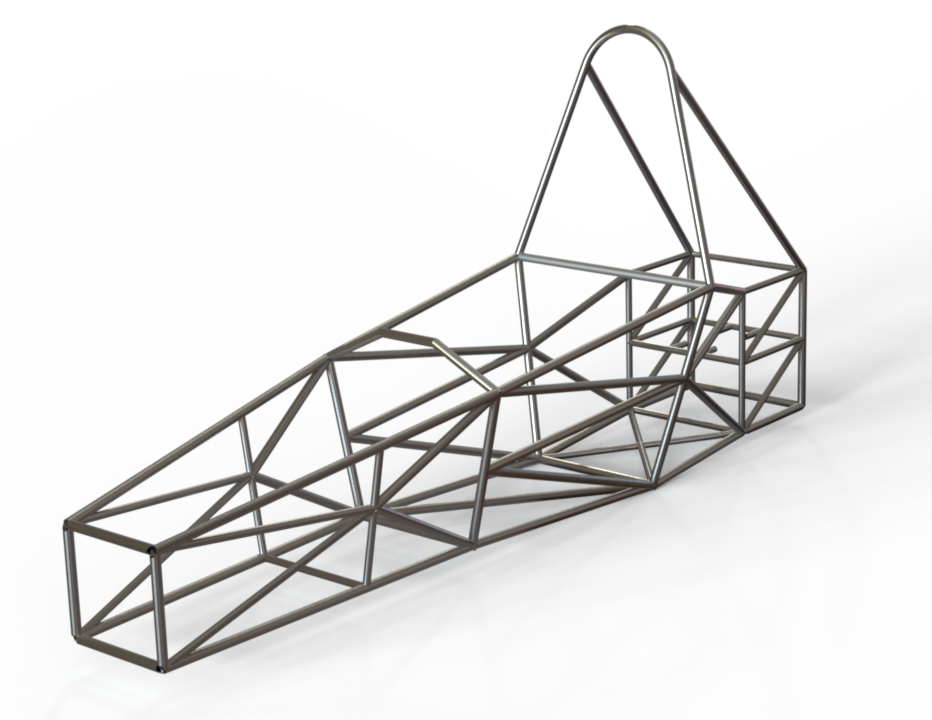
\includegraphics[width=0.48\textwidth]{../TobyMcConnell/Engineering/Images/render.png}
    \caption{Chassis Render}
    \label{fig:Chassis Render}
\end{figure}

The primary performance objective is therefore to create a cost effective structure which minimises total vehicle mass while safely handling high acceleration and high drivetrain torque, whilst also protecting the driver during potential crash scenarios in the most structurally efficient manner.

\section{Design Requirements and Constraints}

The chassis design must satisfy a range of performance targets, structural requirements, and regulatory constraints. These factors collectively define the design space within which the final architecture is developed. The primary aim is to minimise vehicle mass while maintaining structural integrity and regulatory compliance. 

\begin{table}[H]
\centering
\caption{Vehicle performance targets}
\vspace{-8pt}
\label{tab:performance_targets}
\footnotesize
\singlespacing
\begin{tabularx}{\textwidth}{|p{3.2cm}|p{2.2cm}|X|}
\hline
\textbf{Metric} & \textbf{Target} & \textbf{Design Rationale} \\
\hline
Total Vehicle Mass & $<220$ kg & Simulations indicate optimal mass near 170 kg; perfomance only get notably worse at total masses over 220 kg \\
\hline
Chassis Mass & $<48$ kg & Supercapacitors: 38 kg; Front wheels: 2$\times$4.6 kg; Rear wheels: 2$\times$5.0 kg; Motor: 28.2 kg; Inverter: 8.5 kg; Driver: 68 kg, Coolant Oil + Tank: 1kg, Suspension + Bodywork: $\sim$10 kg. For Chassis: $220 - \sum = 43$. \\
\hline
Horizontal CoM (Longitudinal Weight Distribution) & 65--70\% rear & With our Rear-Wheel drive car we want as much as weight as possible over the rear axle to maximise traction and prevent wheel spin but also want enough weight over the front to prevent wheelies and maintaining stability. See Section \ref{sec:wheelbase_mass_distribution}.\\
\hline
Vertical CoM & Minimise & Lower centre of mass improves stability and reduces pitch during acceleration. \\
\hline
Structural Durability & No yielding & Chassis must transmit motor torque and longitudinal acceleration loads without permanent deformation and protect driver in crash scenarios. \\
\hline
Stiffness Priority & Longitudinal & Straight-line optimisation prioritises resistance to longitudinal loads, motor reaction torque and impacts over torsional stiffness. \\
\hline
Chassis Price & Minimise (ideally $<\text{\pounds}1500$) & Keep price as low as possible to maximise second/£ \\
\hline
\end{tabularx}
\end{table}
\vspace{-10pt}

Vehicle performance targets were derived from vehicle dynamics simulation (mass sensitivity to 75m time identified in Section \ref{sec:tornado}) and a component mass budget, the chassis mass was calculated as the residual after allocating mass to all other subsystems. Fabrication cost covers materials only and assumes access to university workshop facilities.  

\section{Chassis Type Selection}

The first major structural design decision was the selection of the overall chassis architecture. 

\begin{itemize}
    \item \textbf{Spaceframe options:}
    \begin{itemize}
        \item A spaceframe is a structure made from interconnected tubes, the default construction for FS is mild steel or alloy tubing.
        \item It can also be constructed using ``Alternative Materials'' as per T3.3 \cite{fsae_rules_2025} - usually, aluminium
    \end{itemize}

    \item \textbf{Alternatives to spaceframe:}
    \begin{itemize}
        \item The most common approved ``Composite Structure'' as per T3.4 \cite{fsae_rules_2025} is a carbon fibre monocoque.
        \item A hybrid structure with different chassis sections using different concepts.
    \end{itemize}

\end{itemize}
 
Each concept offers distinct advantages, in order to objectively evaluate these alternatives, a weighted Pugh decision matrix was used, allowing each concept to be assessed against criteria relevant to the sprint-optimised design objectives (Table \ref{tab:design_pugh}).

\begin{table}[h]
    \centering
    \caption{Architecture Pugh Matrix}
    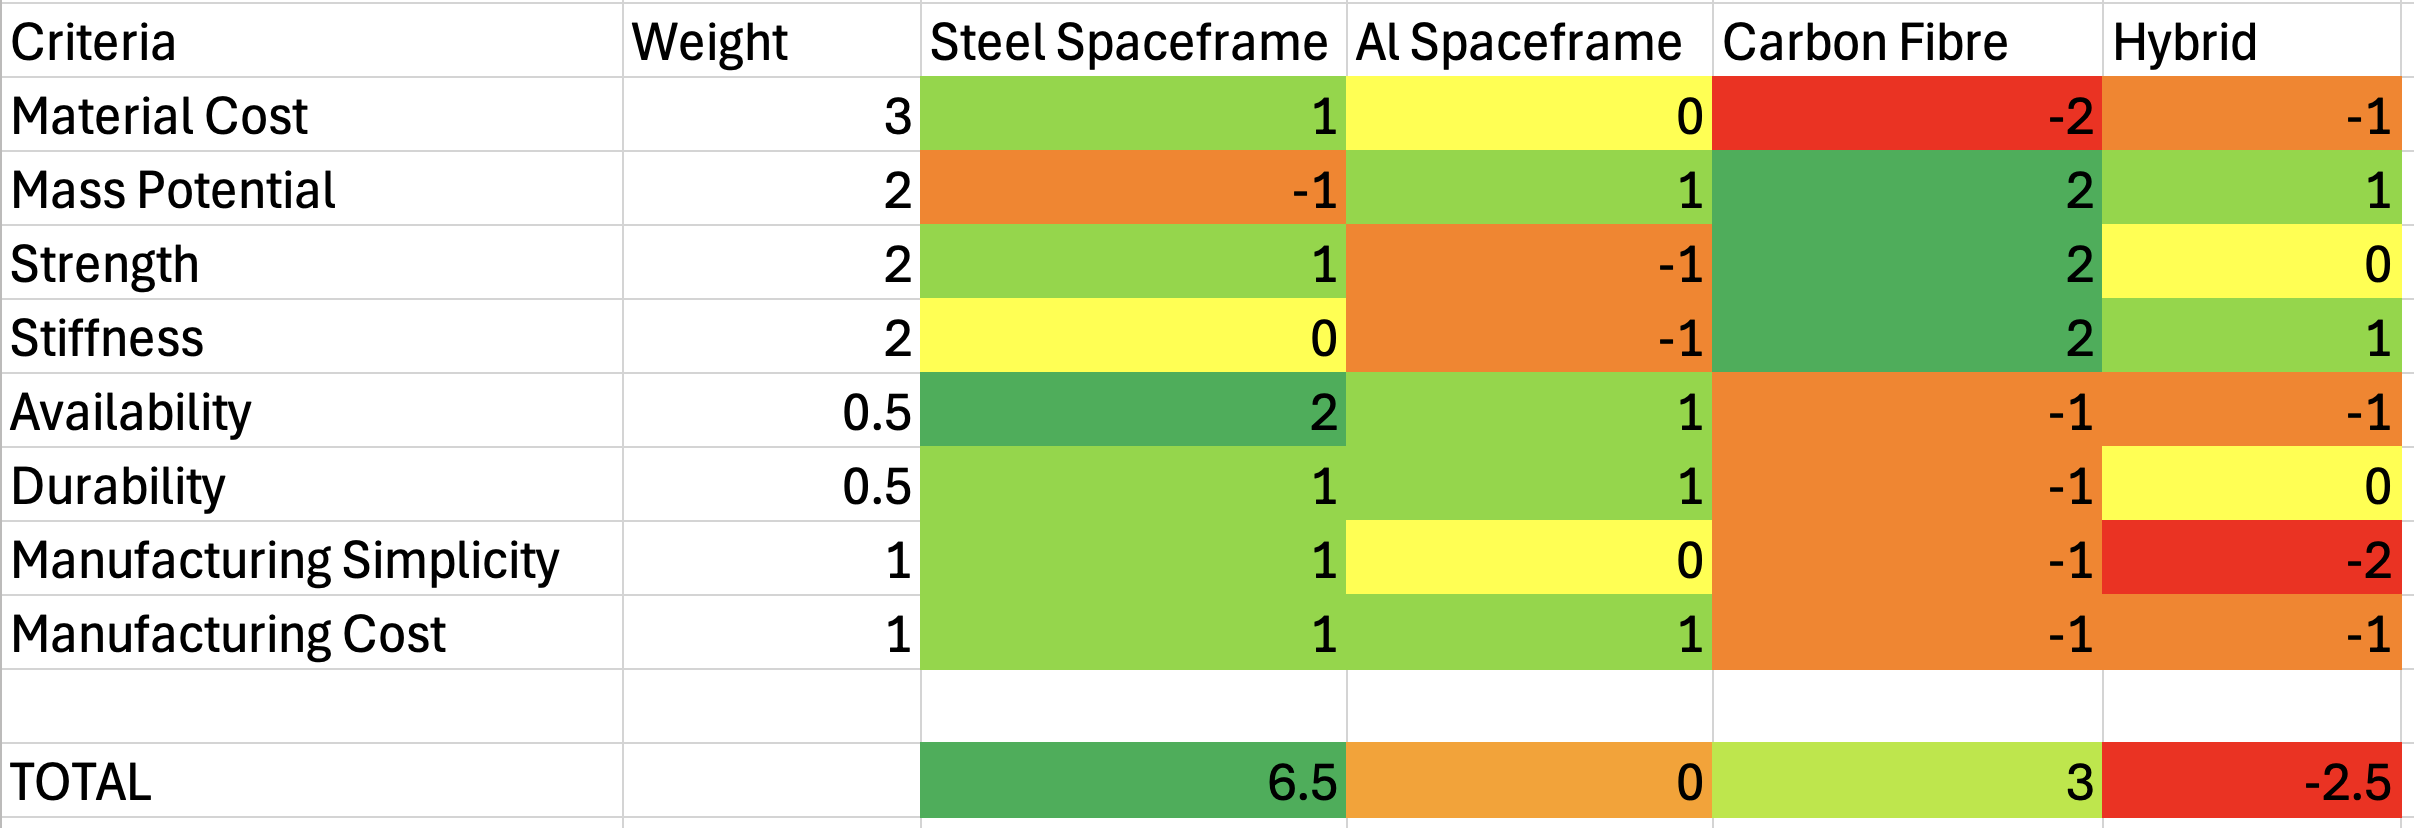
\includegraphics[width=0.8\textwidth]{../TobyMcConnell/Engineering/Images/Design_Pugh.png}
    \label{tab:design_pugh}
\end{table}

Weighting is heavily biased toward Cost and Manufacturing. Table \ref{tab:chassis_cost_performance} illustrates the reasoning by the low weight rating for mass potential in the Pugh matrix due to its minimal impact on perfomance within the range of different chassis masses.

\begin{table}[h]
\centering
\caption{Cost-per-second of improvement for Lighter Chassis Option}
\label{tab:chassis_cost_performance}
\begin{tabular}{|l|c|c|c|c|}
\hline
\textbf{Chassis Type} & \makecell{\textbf{Weight Est.} \\ \textbf{(kg)}} & \makecell{\textbf{Price Est.} \\ \textbf{(£)}} & \makecell{\textbf{Finish Time Est.} \\ \textbf{(s)}} & \makecell{\textbf{£ per s} \\ \textbf{lost}} \\
\hline
Heavy Steel Spaceframe (Baseline) & 50 & 1000 & 3.60 & -- \\
Light Carbon Monocoque & 20 & 2500 & 3.56 & 37500 \\
\hline
\end{tabular}
\end{table}

Strength was considered to ensure driver safety, perfomance in crashes, and compliance with regulations. Stiffness is typically prioritised in circuit-focused vehicles to improve cornering performance, but this is less critical for a drag-optimised design. It was still assigned a rating of 2, as sufficient stiffness is required to ensure drivetrain loads are efficiently transferred to the wheels rather than being absorbed through chassis deflection. Material Cost, Availability, and Manufacturing Simplicity factors ensure focus on a practical, cost-efficient design. The Steel Spaceframe scored highest in the Pugh Matrix and was selected as offering the most balanced approach. It traded marginal performance gains of composites for reliability, simplicity and price \cite{racecar_engineering_oxford_brookes} \cite{tutf_composite_build}.

\section{Material Selection}

Having selected the Steel Spaceframe design, it is necessary to determine the exact steel alloy. Four options were considered, based on the prevalenceof use in race car chassis: 
%\vspace{-5pt}
\begin{itemize}
    \item \textbf{Mild Steel (CDS):} A low-carbon steel with good ductility, weldability, 
    and availability.

    \item \textbf{AISI 1020 Cold Drawn Steel:} A medium-low carbon steel with improved 
    strength and dimensional consistency compared to standard mild steel due to the 
    cold-drawing process. 

    \item \textbf{4130 Chromoly:} A low-alloy steel containing chromium and molybdenum as 
    strengthening agents, traditionally used in aviation and professional motorsports.

    \item \textbf{Docol R8:} A modern dual-phase advanced high-strength steel (AHSS) 
    engineered to provide a consistent grain structure, high strength, and improved 
    energy absorption characteristics.
\end{itemize}
%\vspace{-15pt}
\subsection{Mass, Cost, and Manufacturing Analysis}

As a material choice, higher yield strength steels offer mass reduction potential because thinner tubing can be used while still meeting FS bending and safety requirements. However, this benefit is limited since all steels share a similar Young’s Modulus, meaning thinner tubes are inherently less stiff. Therefore, FS equivalency rules reduce any advantage by requiring larger diameters to restore bending stiffness, offsetting much of the initial mass saving.

Using a preliminary CAD model for the Steel Spaceframe built on SolidWorks using weldments software and custom material and tube packages, material options were compared (Table \ref{tab:chassis_materials}).

\begin{table}[h]
    \centering
    \caption{Comparison of candidate chassis materials}
    \label{tab:chassis_materials}
    \footnotesize
    \begin{tabular}{|l|c|c|c|c|c|}
        \hline
        \textbf{Material} & \makecell{\textbf{Est. Chassis} \\ \textbf{Mass (kg)}} & \makecell{\textbf{Material} \\ \textbf{Cost (£)}} & \makecell{\textbf{Strength} \\ \textbf{(MPa)}} & \makecell{\textbf{Performance} \\ \textbf{Est. (s)}} & \makecell{\textbf{Mfg.} \\ \textbf{Complexity}} \\
        \hline
        {Mild Steel (CDS)}\cite{rapidmetals_mild_steel_tube} & 40 & 480 & 280 & 3.59 & Low (MIG) \\
        {AISI 1020 CD}\cite{matweb_aisi1020} & 40 & 550 & 420 & 3.59 & Low (MIG) \\
        {4130 Chromoly}\cite{weldracing_25crmo4} & 31 & 1,050 & 560 & 3.57 & High (TIG + HAZ) \\
        {Docol R8}\cite{aedmetals_docol_r8} & 30 & 1,200 & 800 & 3.57 & Moderate (TIG/MIG) \\
        \hline
    \end{tabular}
\end{table}

The 4130 chromoly material choice requires careful welding heat input and cooling rate control to avoid embrittlement in the heat-affected zone. This impacted the manufacturing complexity scores, as its use would require TIG welding and greater operator skill. Docol R8, while less sensitive to heat-affected zone effects, has very high strength and hardness which increases tool wear during cutting, drilling, and notching \cite{millerwelds2024}.

\subsection{Pugh Matrix and Final Material Selection}

\begin{table}[h]
    \centering
    \caption{Steel Pugh Matrix}
    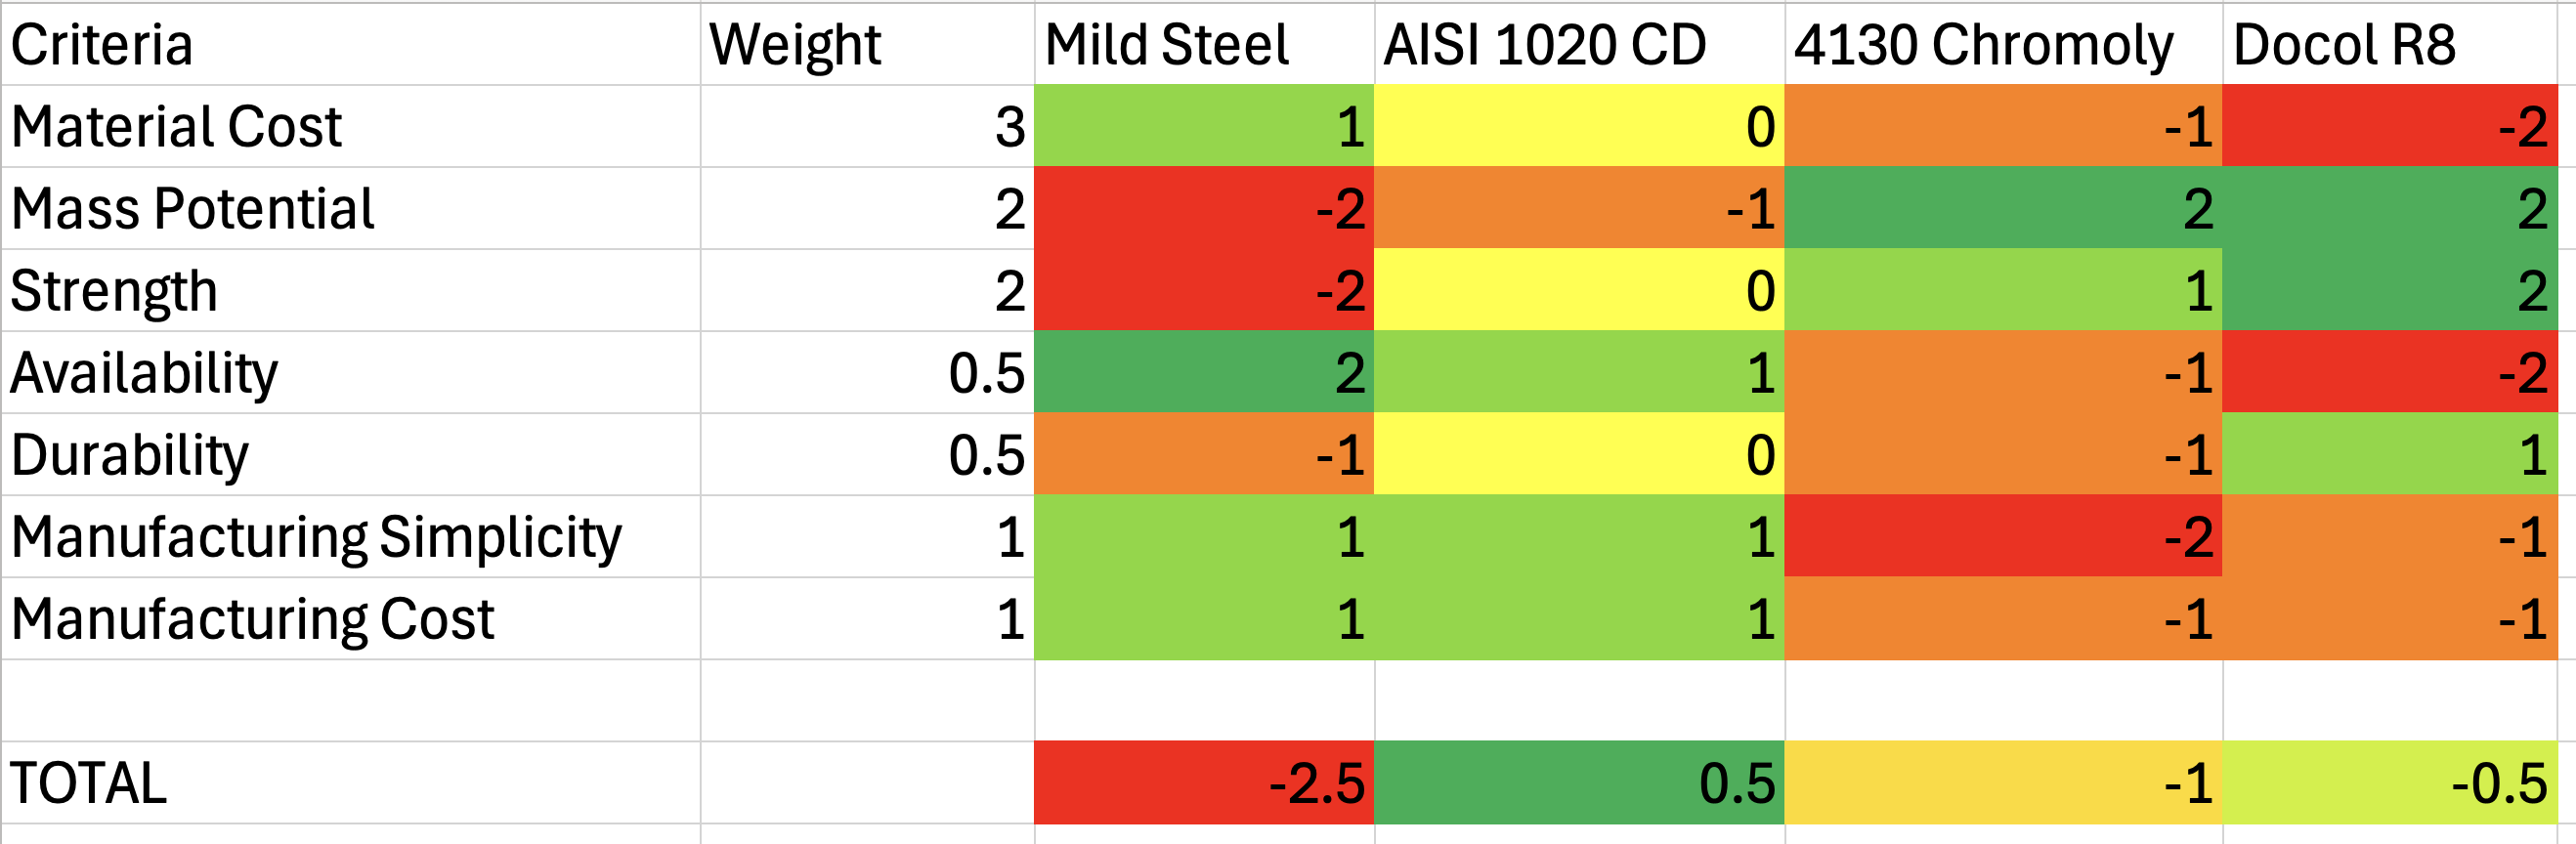
\includegraphics[width=0.8\textwidth]{../TobyMcConnell/Engineering/Images/Steel_pugh.png}
    \label{tab:steel_pugh}
\end{table}

To finalize material selection we used the same Pugh matrix (with stiffness removed as it is uniform across steel alloys). We opted for AISI 1020 CD, it provides a 350--380 MPa yield strength (50\% higher than standard mild steel) and is cheap and easy to MIG weld. This sacrifices marginal performance improvements to avoid the high costs and complexities of the higher-end alloys. Additionally, the higher strengths of the 4130 Chromoly and Docol R8 are often limited by the weld and heat-affected zone, which typically has similar strength regardless of the parent material, reducing their benefit. To finalise material design, we conducted a separate analysis of tube size and structure, as set out in Table \ref{tab:tube_diameter_strategy}

\begin{table}[h]
    \centering
    \caption{Tube diameter strategy}
    \label{tab:tube_diameter_strategy}
    \footnotesize
    \begin{tabular}{|p{2.75cm}|c|p{4.2cm}|p{6.2cm}|}
        \hline
        \textbf{Structure} & \makecell{\textbf{Tube Size} \\ \textbf{(mm)}} & \textbf{Rule / Requirement} & \textbf{Application Rationale} \\
        \hline
        Main Roll Hoop & 25 $\times$ 2.5 & Primary structures must meet baseline roll-over strength requirements. & Thickest wall section used to maximise safety factor during rollover events and provide highest bending resistance. \\
        \hline
        Front Hoop and Side Impact & 25 $\times$ 2.0 & Cockpit protection structures subject to impact loading requirements. & Protects driver's cockpit; AISI 1020 CD provides $\sim$350 MPa yield capacity per tube. Members primarily experience compression during collisions, so 2 mm wall thickness reduces buckling risk. \\
        \hline
        Secondary Bracing & 20 $\times$ 2.0 & No direct regulatory requirement for non-impact structural members. & Used for non-critical bracing to reduce mass while maintaining adequate stiffness. See \ref{sec:chassis_architecture} \\
        \hline
    \end{tabular}
\end{table}
\vspace{-16pt}

\section{Chassis Architecture}
\label{sec:chassis_architecture}
After selecting the Steel Spaceframe architecture, the design process focused on optimising packaging to create a compact, lightweight chassis built around the driver and components.

The cockpit was designed first, positioning the front bulkhead, side impact structure, and roll hoops around the “Percy” driver template -- a 95th percentile male defined in FS regulations. The front and main roll hoops were then integrated to provide rollover protection and form key structural nodes. Once the driver envelope was defined, the powertrain components (i.e. supercapacitors, inverter, and motor) were packaged in the rear of the chassis (fig. \ref{fig:components}). Locating these components close together reduced cabling length, helped concentrate the centre of mass near the rear axle and allowed one simple firewall to be placed directly behind the driver to meet FS regulations. The rear was also designed with a large enough opening below the supercapacitors with removable support bars, making it easy to take in and out for safety checks and maintenance. This layout was enabled by the rear-wheel-drive configuration. The motor mount was then integrated directly into triangulated members to ensure torque loads are efficiently transferred into the chassis without introducing excessive bending stresses (verified in Section \ref{sec:motor_torque_load_case}). The mounting for the rest of the components is more trivial with base plates and clamps that were deemed unnecessary to fully design as they had little effect on chassis performance, however their exact mount points in the chassis were identified and used for simulating the effect of their mass in section \ref{sec:static_acc_load}.

Once the frame geometry was established the secondary tubes were identified and converted from 25x2mm to 20x2mm leading to a total 2kg mass reduction (fig. \ref{fig:thin_bars}).

\begin{figure}[htbp]
    \centering
    \begin{subfigure}{0.47\textwidth}
        \centering
        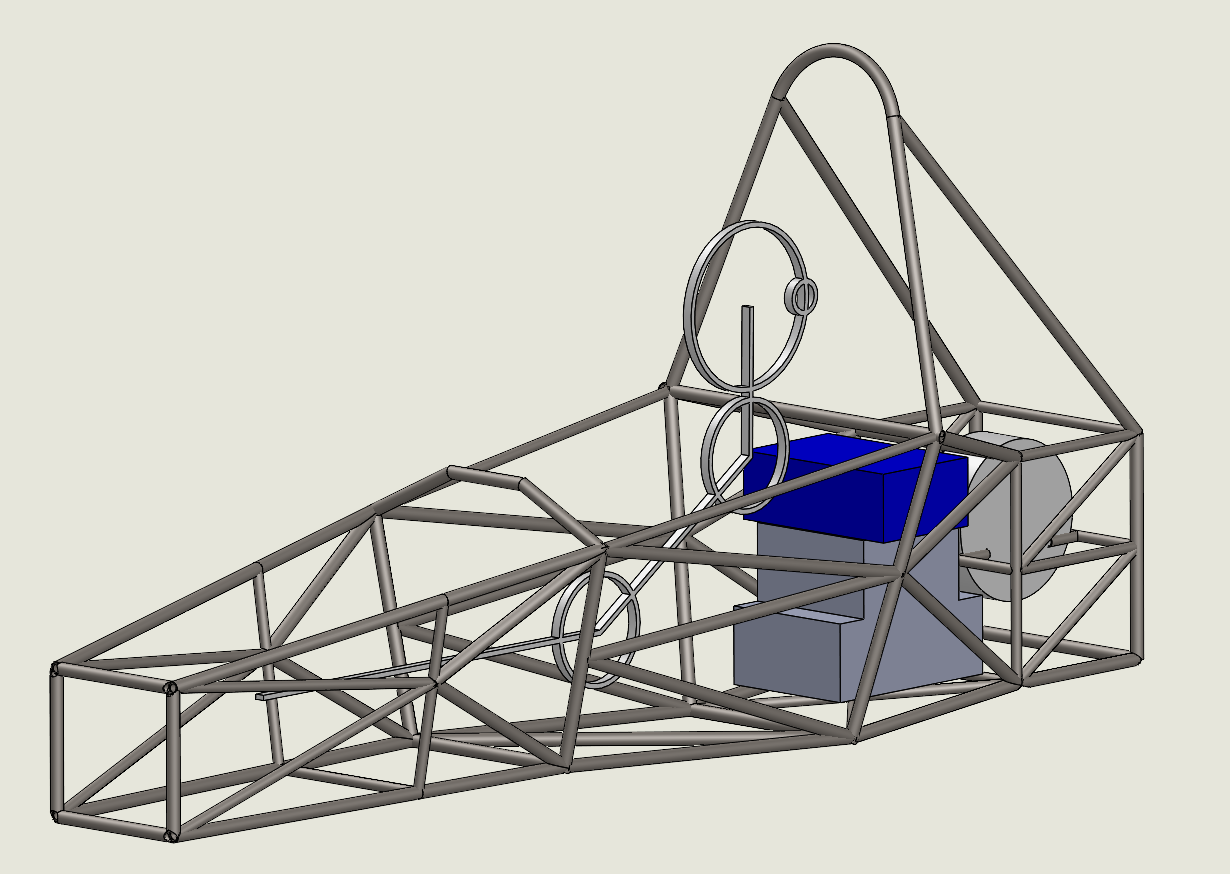
\includegraphics[width=\linewidth]{Images/components.png}
        \caption{Chassis with components}
        \label{fig:components}
    \end{subfigure}
    \hfill
    \begin{subfigure}{0.5\textwidth}
        \centering
        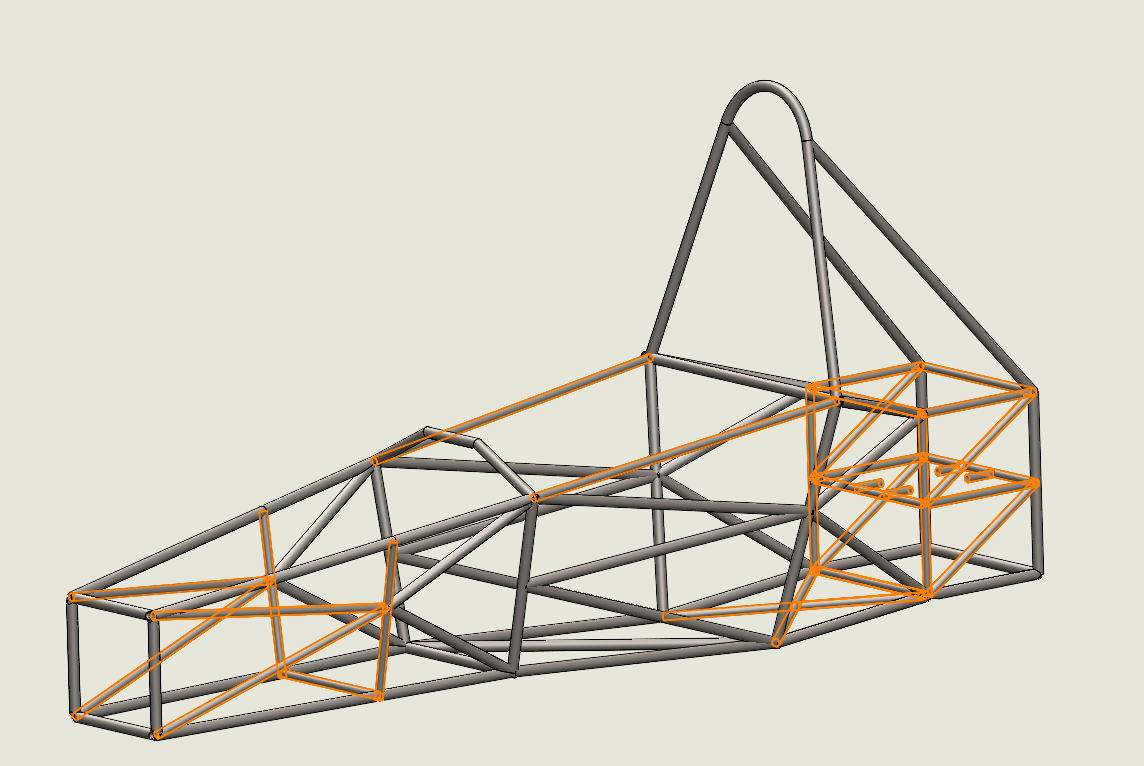
\includegraphics[width=\linewidth]{Images/thin_bars.png}
        \caption{Bars Replaced with 20x2mm tubes}
        \label{fig:thin_bars}
    \end{subfigure}
    \caption{Preliminary Operational Load Cases}
    %\label{fig:both}
\end{figure}
\vspace{-16pt}
\subsection{Impact Attenuator}

The FS standard impact attenuator (IA) \cite{fsae_rules_2025} was selected because it offers excellent energy absorption and proven reliability \cite{dewesoft2025ia}, enhancing driver safety with minimal weight penalty. Designing and verifying a custom IA would add significant cost, complexity, and testing requirements, while the relatively low risk of high-energy crashes in our sprint-focused chassis means that a standard, approved attenuator provides a safer and more efficient solution. Although using the standard IA results in a small points penalty, the benefits in reduced risk, cost, and development effort make a custom design unjustifiable.

\subsection{Wheelbase}
\label{sec:wheelbase_mass_distribution}

A crucial aim of the chassis design is to ensure our car avoids wheelieing (front wheel lifting off the ground) during the high acceleration of the event. This is because lifting the front wheels reduces steering control and wastes energy raising the vehicle’s centre of mass instead of accelerating forward. Using the CAD model: including chassis, driver and all components for the  CoM estimates, the wheelie limit can be estimated by balancing moments about the rear axle. A wheelie occurs when the front axle load becomes zero, which leads to the relationship:
\vspace{-1pt}
\begin{equation}
    a = g \times \frac{d_{\text{rear}}}{h}
\end{equation}

where \( a \) is vehicle acceleration, \( d_{\text{rear}} \) is the horizontal distance between the centre of mass and the rear axle, and \( h \) is the centre of mass height.

Rearranging the equation allows the minimum distance from the centre of mass to the rear axle to be calculated for the vehicle’s predicted peak acceleration of 1.33 \( g\). With an estimated centre of mass height of 325 mm based on first iteration in CAD, the required distance becomes:
 \vspace{-2pt}
\begin{equation}
    d_{\text{rear}} = \frac{a}{g} \times h = 1.33 \times 0.325\,\text{m} \approx 0.432\,\text{m}
\end{equation}

Therefore, the centre of mass must be located at least 432 mm forward of the rear axle to prevent front wheel lift under maximum acceleration.

\subsection{Suspension Hardpoints}

A 200 ± 50 mm by 450 ± 100 mm template provided by the wheel team was used to guide the geometry of the chassis, Four triangulated nodes were situated at each corner of the area for placement of suspension mounting points. Roll hoops are designed primarily as safety structures; and therefore the main roll hoop was not used for rear suspension mounting to avoid introducing operational loads that could compromise rollover protection. Instead, the rear of the chassis was extended behind the main roll hoop to provide suitable mounting locations for the rear suspension. The front of the chassis was optimised to minimise structural mass. The front suspension mounting points were integrated into the front roll hoop structure, where loads can be effectively triangulated into the surrounding members, allowing the roll hoop to contribute structurally without compromising its safety function. This approach reduces the need for additional forward chassis members and lowers overall mass. Both decisions offer the added benefit of shifting the centre of mass slightly rearward, closer to our target of 70\% while remaining within wheelie limits. Space was also reserved beneath the drivers' legs at the front of the chassis to accommodate the steering rack. Table \ref{tab:layout_summary} shows the final layout calculations

\begin{table}[h]
    \centering
    \caption{Final chassis layout and mass distribution summary}
    \label{tab:layout_summary}
    \begin{tabular}{|l|c|}
        \hline
        \textbf{Parameter} & \textbf{Value} \\
        \hline
        Wheelbase & 1573 mm \\
        Centre of Mass Height & 325 mm (from CAD) \\
        CoM Distance Ahead of Rear Axle & 481 mm (from CAD) \\
        Wheelie Safety Factor (vs. max launch) & $< 0.9$ \\
        Front Weight Distribution & 30.5 \% \\
        Rear Weight Distribution & 69.5 \% \\
        \hline
    \end{tabular}
\end{table}
\vspace{-16pt}
\section{Manufacturing and Structural Integrity Report}

When constructing the chassis, weld strength is critical. The principal aim for the analysis in this section is to ensure that during chassis failure the tube reaches yield before weld failure. Yielding of the tube is preferred because plastic deformation of the parent material absorbs a large amount of energy and allows loads to redistribute through the spaceframe, whereas weld failure is typically more brittle and can cause a sudden loss of load path at a joint, potentially leading to local separation of members and intrusion into the driver survival space. This is more dangerous in a chassis failure scenario. The weld capacity and yield calculations are as follow in section \ref{sec:tube_weld_capacity}.
\subsection{Tube and Weld Capacity Calculation}
\label{sec:tube_weld_capacity}
\noindent\textbf{Tube Properties}\par
\vspace{4pt}
\begin{table}[h]
    \centering
    \begin{tabular}{|l|c|}
        \hline
        Parameter & Value \\
        \hline
        Yield Strength, $\sigma_y$ & $350\ \text{MPa}$ \\
        Ultimate Strength, $\sigma_u$ & $420\ \text{MPa}$ \\
        Outer Diameter, $D$ & $25\ \text{mm}$ \\
        Wall Thickness, $t$ & $2\ \text{mm}$ \\
        Inner Diameter, $d$ & $21\ \text{mm}$ \\
        \hline
    \end{tabular}
\end{table}
\vspace{6pt}

\noindent\textbf{Tube Section Properties}\par
\vspace{4pt}
\begin{align*}
A &= \frac{\pi}{4}(D^2 - d^2)
= \frac{\pi}{4}(25^2 - 21^2)
= 144.5\ \text{mm}^2 \\
Z &= \frac{\pi (D^4 - d^4)}{32D}
= \frac{\pi (25^4 - 21^4)}{32 \times 25}
= 763.5\ \text{mm}^3
\end{align*}

\noindent\textbf{Tube Capacity}\par
\vspace{4pt}
\begin{align*}
F_{\text{tube}} &= A \sigma_y
= 50\,575\ \text{N} \ (50.6\ \text{kN}) \\
M_{\text{tube}} &= Z \sigma_y
= 267\,225\ \text{N·mm} \ (267.2\ \text{Nm})
\end{align*}

\noindent\textbf{Weld Properties}\par
\vspace{4pt}
\begin{table}[h]
    \centering
    \begin{tabular}{|l|c|}
        \hline
        Parameter & Value \\
        \hline
        Fillet Size, $w$ & $3.5\ \text{mm}$ \\
        Effective Throat, $t_e$ & $2.47\ \text{mm}$ \\
        Allowable Shear, $\tau_{\text{allow}}$ & $300\ \text{MPa}$ \\
        \hline
    \end{tabular}
\end{table}
\vspace{6pt}

\noindent\textbf{Weld Capacity}\par
\vspace{4pt}
\begin{align*}
A_w &= \pi D t_e
= 194.0\ \text{mm}^2 \\
Z_w &= \pi r_{\text{mean}}^2 t_e
= 1026.3\ \text{mm}^3 \\
F_{\text{weld}} &= A_w \tau_{\text{allow}}
= 58\,200\ \text{N} \ (58.2\ \text{kN}) \\
M_{\text{weld}} &= Z_w \tau_{\text{allow}}
= 307\,890\ \text{N·mm} \ (307.9\ \text{Nm})
\end{align*}

\vspace{6pt}

\begin{table}[H]
    \centering
    \caption{Comparative safety margin between tube and weld capacities.}
    \vspace{-12pt}
    \label{tab:weld_vs_tube}
        \footnotesize
        \singlespacing
        \begin{tabular}{|l|c|c|c|}
        \hline
        \textbf{Load Type} & \textbf{Tube Yield Capacity} & \textbf{Weld Capacity (3.5 mm)} & \textbf{Failure Sequence} \\
        \hline
        Axial Force & 50.6 kN & 58.2 kN & Tube Fails First \\
        Bending Moment & 267.2 Nm & 307.9 Nm & Tube Fails First \\
        \hline
    \end{tabular}
\end{table}

Having justified weld safety, practical fabrication considerations were addressed to maximise the quality of the chassis construction. The design features a lot of multi-member nodes, where up to five tubes intersect. This introduces geometric interference that restricts MIG torch (welding gun) access and increases the risk of poor penetration. To manage this, eccentricities or slight offsets between tubes are introduced to maintain weld accessibility. These nodes also act as large heat sinks, creating thermal distortion during cooling. This is mitigated through a balanced welding sequence applied in staggered increments to distribute heat evenly. A controlled bottom-up fabrication workflow is used. First, the floor structure is jigged on a flat table with dummy suspension tabs to establish a rigid reference plane. Then precision hole-saw notching and CAD generated templates are usedfor the complex joints, such as in the roll hoops. Finally, full chassis tacking prior to final welding to verify squareness and maintain suspension hardpoint tolerances. See table \ref{tab:chassis_cost_breakdown} for the estimated total cost of this construction.

\begin{table}[h]
    \centering
    \caption{Estimated fabrication cost breakdown for chassis.}
    \label{tab:chassis_cost_breakdown}
    \footnotesize
    \begin{tabular}{|l|l|c|}
        \hline
        \textbf{Category} & \textbf{Item Description} & \textbf{Estimated Cost} \\
        \hline
        Raw Material & 30m of AISI 1020 CD Tubing \cite{matweb_aisi1020} & £550 \\
        Welding Gas & 1x Large Bottle Argon/CO$_2$ & £90 \\
        Filler Metal & 5kg Spool ER70S-6 MIG Wire & £30 \\
        Consumables & Hole-saws, Flap discs, Sanding belts & £80 \\
        Jigging & MDF/Steel scrap, clamps, and fasteners & £70 \\
        Impact Attenuator & FSAE Standard Impact Attenuator \cite{fsae_impact_attenuator} & £113 \\
        \hline
        \textbf{TOTAL} &  & \textbf{£833} \\
        \hline
    \end{tabular}
\end{table}

\section{Chassis Performance Verification with Finite Element Analysis}

The final step in the verification was to simulate all use case scenarios for the chassis to verify and optimise its design. This was done by using Finite Element Analysis (FEA) \cite{irjet2019fea} in SolidWorks: FEA divides the chassis into a mesh of small elements and calculating stresses, deflections, and potential failure points for each of these elements we can accurately predict the overall behaviour under different load cases.

Each simulation was evaluated against three key failure modes to ensure the chassis design meets the required safety and performance standards:

\begin{itemize}
    \item \textbf{Yielding:} The initial FEA assessment focused on identifying stresses exceeding the design limit of S.F. = 0.9 $\cdot \sigma_y$ (using $\sigma_y$ from \cite{matweb_aisi1020}). This kind of localised yielding in extreme crash scenarios was not considered critical, as limited plastic deformation is acceptable provided driver safety is maintained. The low likelihood of such events justifies potential repair costs.
    \item \textbf{Buckling:} All simulations were checked for excessive compressive loads in members, since buckling can occur below the material yield strength. This represents a mechanical instability rather than a material failure, meaning a member can suddenly lose load-carrying capacity without the material itself yielding, making it a more abrupt and dangerous failure mode. 
    \item \textbf{Weld Stresses:} Weld stresses were monitored separately, with an allowable limit defined using a S.F. $\sim 0.75$ but dependent on the complexity of the weld. As stated earlier, weld failure is particularly dangerous as it can result in complete separation of members and immediate loss of structural load paths.
\end{itemize}

It is important to note that lateral stiffness simulations were not deemed necessary. These simulations are crucial for analysing ability of the chassis during turning at high speeds but are not at all necessary for our acceleration event where no turning occurs.

\subsection{Static and Acceleration Simulations}
\label{sec:static_acc_load}

\begin{figure}[htbp]
    \centering
    \begin{subfigure}{0.475\textwidth}
        \centering
        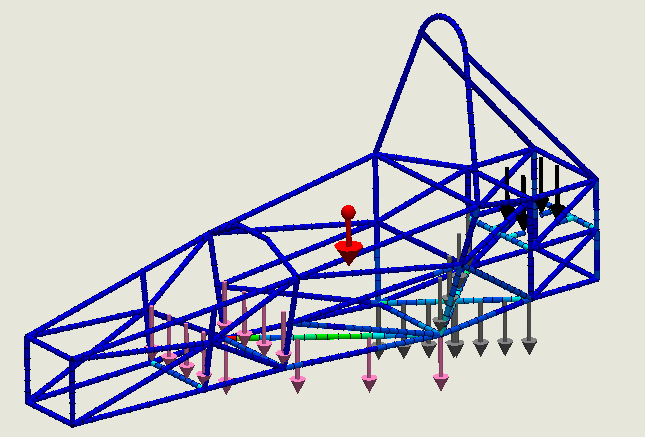
\includegraphics[width=\linewidth]{Images/resting_forces.png}
        \caption{Resting forces}
        \label{fig:resting_forces}
    \end{subfigure}
    \hfill
    \begin{subfigure}{0.48\textwidth}
        \centering
        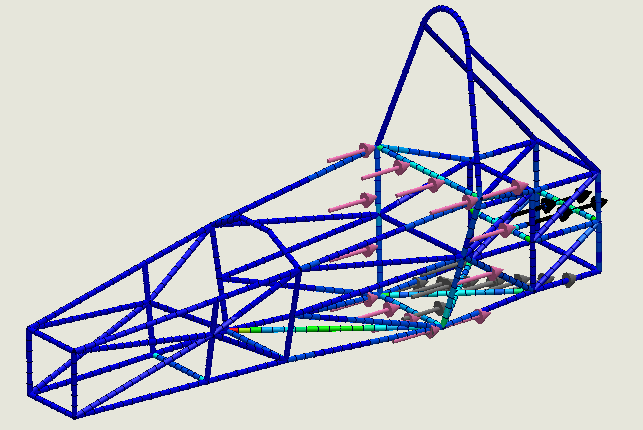
\includegraphics[width=\linewidth]{Images/acceleration_forces.png}
        \caption{Acceleration forces}
        \label{fig:acceleration_forces}
    \end{subfigure}
    \caption{Preliminary Operational Load Cases}
    %\label{fig:both}
\end{figure}

\noindent\textbf{Resting Load Case.}
The first simulation considered the static resting condition of the vehicle. This load case represents the forces acting on the chassis due to the weight of the chassis itself (red), driver (pink), motor (black), and inverter + coolant + supercapacitors (grey) when the car is stationary (fig. \ref{fig:resting_forces}) .
These loads were included in all of the following simulations to ensure their accuracy.

\noindent\textbf{Acceleration Load Case.}\label{sec:acceleration_load_case}
The primary operational load case for a sprint-optimised vehicle is the longitudinal force generated during maximum acceleration. When the vehicle accelerates, inertia produces a rearward force on the chassis that must be resisted by the structural members connecting the drivetrain and suspension mounts.
This force was calculated using Newton’s second law: $F = m \cdot a$ Where m is each components mass. Using the simulated peak acceleration: a = 1.33 \( g\), the resulting force was applied through the drivetrain mounting points and transmitted through the frame toward the suspension nodes.
This load case showed little impact on the chassis which ensured it is more than capable for the acceleration event. 
\subsection{Motor Torque Load Case}
\label{sec:motor_torque_load_case}

The electric motor, which is mounted directly onto our chassis via a lockblot (a vibration proof fastener), produces a high level of torque which is reacted through the motor mounting structure. This creates a torsional load on the surrounding chassis members, which was modelled by applying the predicted maximum motor torque at the motor mounting points at the same time as the acceleration forces in section \ref{sec:acceleration_load_case}. The forces generated by the motor are calculated as: 
\begin{align*}
\text{Max Torque at start: } & T = 370~\text{Nm}, \\
\text{Distance between mounts: } & D = 170~\text{mm} = 0.17~\text{m} \\
\text{Force: } & F = \frac{T}{D} = \frac{370}{0.17} = 2176~\text{N} \\
\text{Force on each front support (red arrow): } & F_{\text{front}} = \frac{F}{2} = 1088~\text{N (up)} \\
\text{Force on each rear support (red arrow): } & F_{\text{rear}} = \frac{F}{2} = 1088~\text{N (down)}
\end{align*}

\begin{figure}[h]
    \centering
    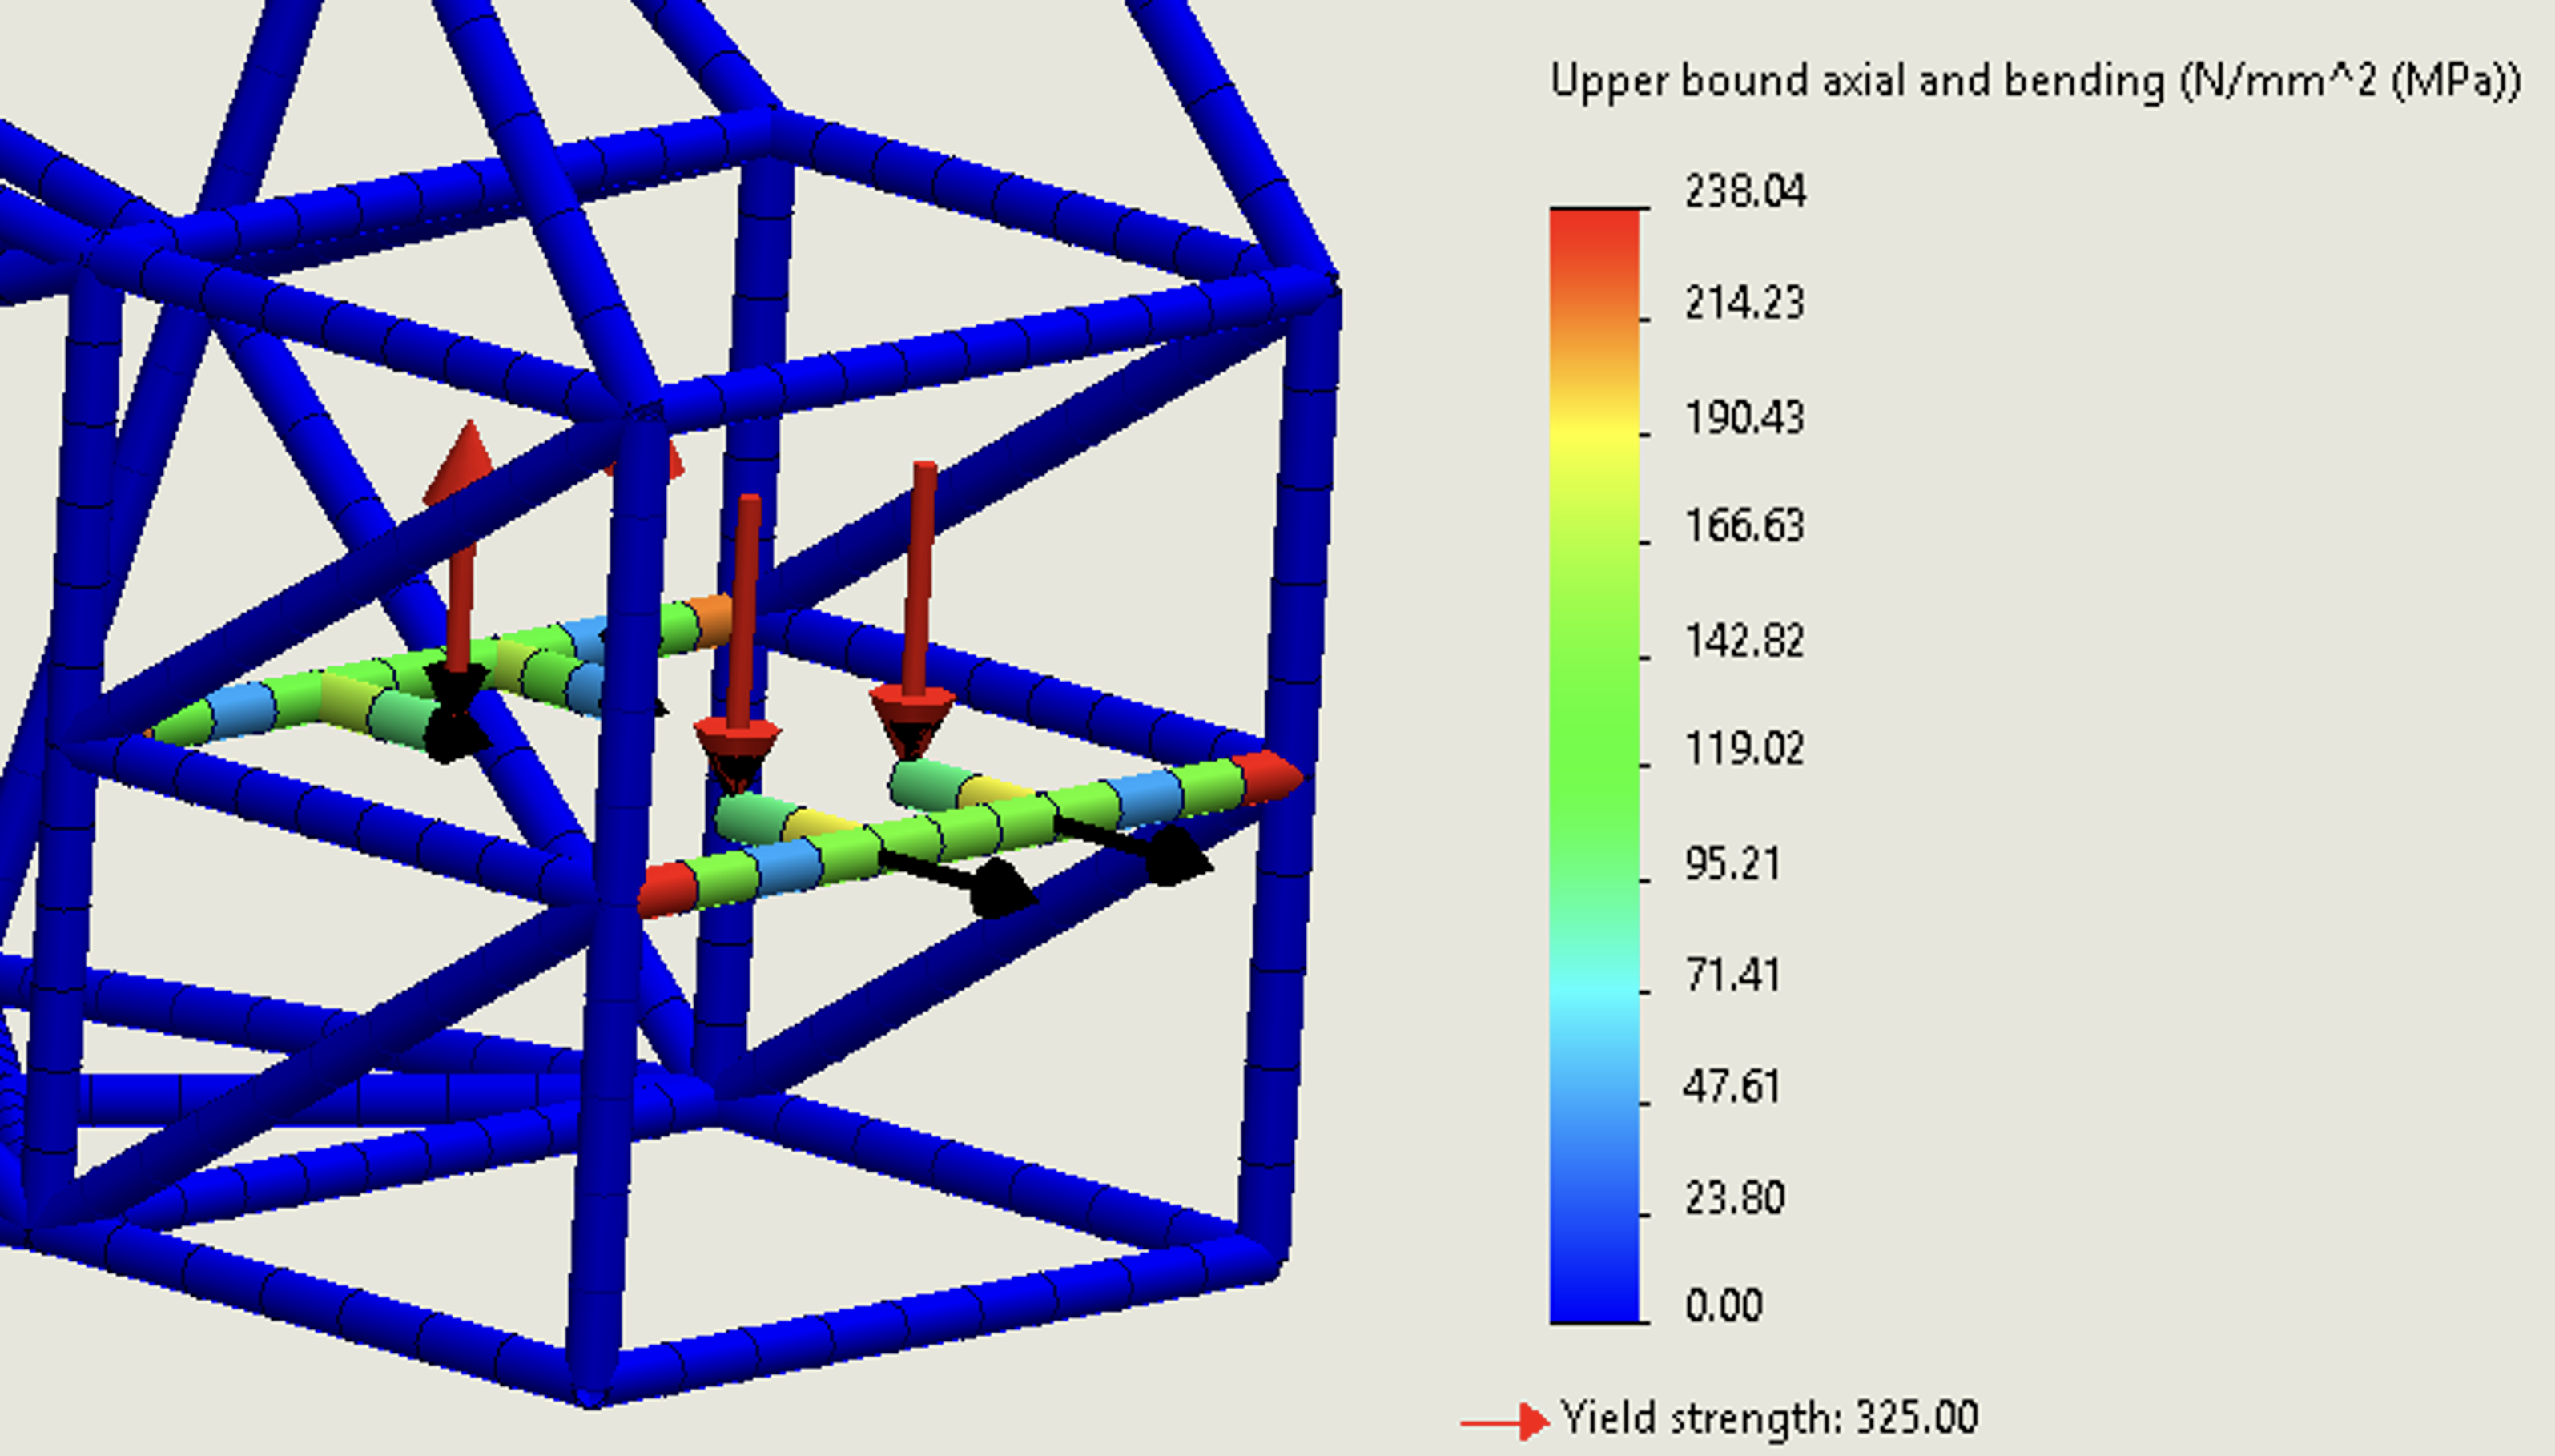
\includegraphics[width=0.75\textwidth]{../TobyMcConnell/Engineering/Images/torquefinal.png}
    \caption{Motor Mount Stress Distribution}
    \label{fig:motor_mount_stress}
\end{figure}

This simulation (fig. \ref{fig:motor_mount_stress}) produced a much higher stress (238Mpa) but was still safely within our yield, compressive force and weld criteria. This is crucial as it ensures the motor is not close to ripping itself out of its mounts during the sprint.

In large vehicles such as trucks, drivetrain torque can sometimes also produce significant global chassis torsion, requiring the entire frame to resist twisting loads. However, the configuration used in this vehicle differs significantly. The motor is mounted with its axis parallel to the driven wheels, meaning the primary torque reaction acts along the longitudinal axis of the vehicle.
As the chassis is much stiffer in the longitudinal direction due to the triangulated spaceframe structure, the resulting torsional deformation of the full chassis is relatively small ($ <<1mm $ of displacement) and therefore, not a concern.

\subsection{Front Impact Simulation}

A front impact scenario was analysed to evaluate the ability of the chassis to protect the driver during a collision. The back of the car was fixed and a front impact of 120kN was applied and evenly distributed across the four corners of the front where the IA will be mounted. This force was based on the FS rule T3.18.3 that states that we "must prove that the AIP can withstand a load of 120kN". This number is designed to represent the highest force the the IA can transmit to the chassis during a worst case head-on collision using the standard FS IA.

\begin{figure}[h]
    \centering
    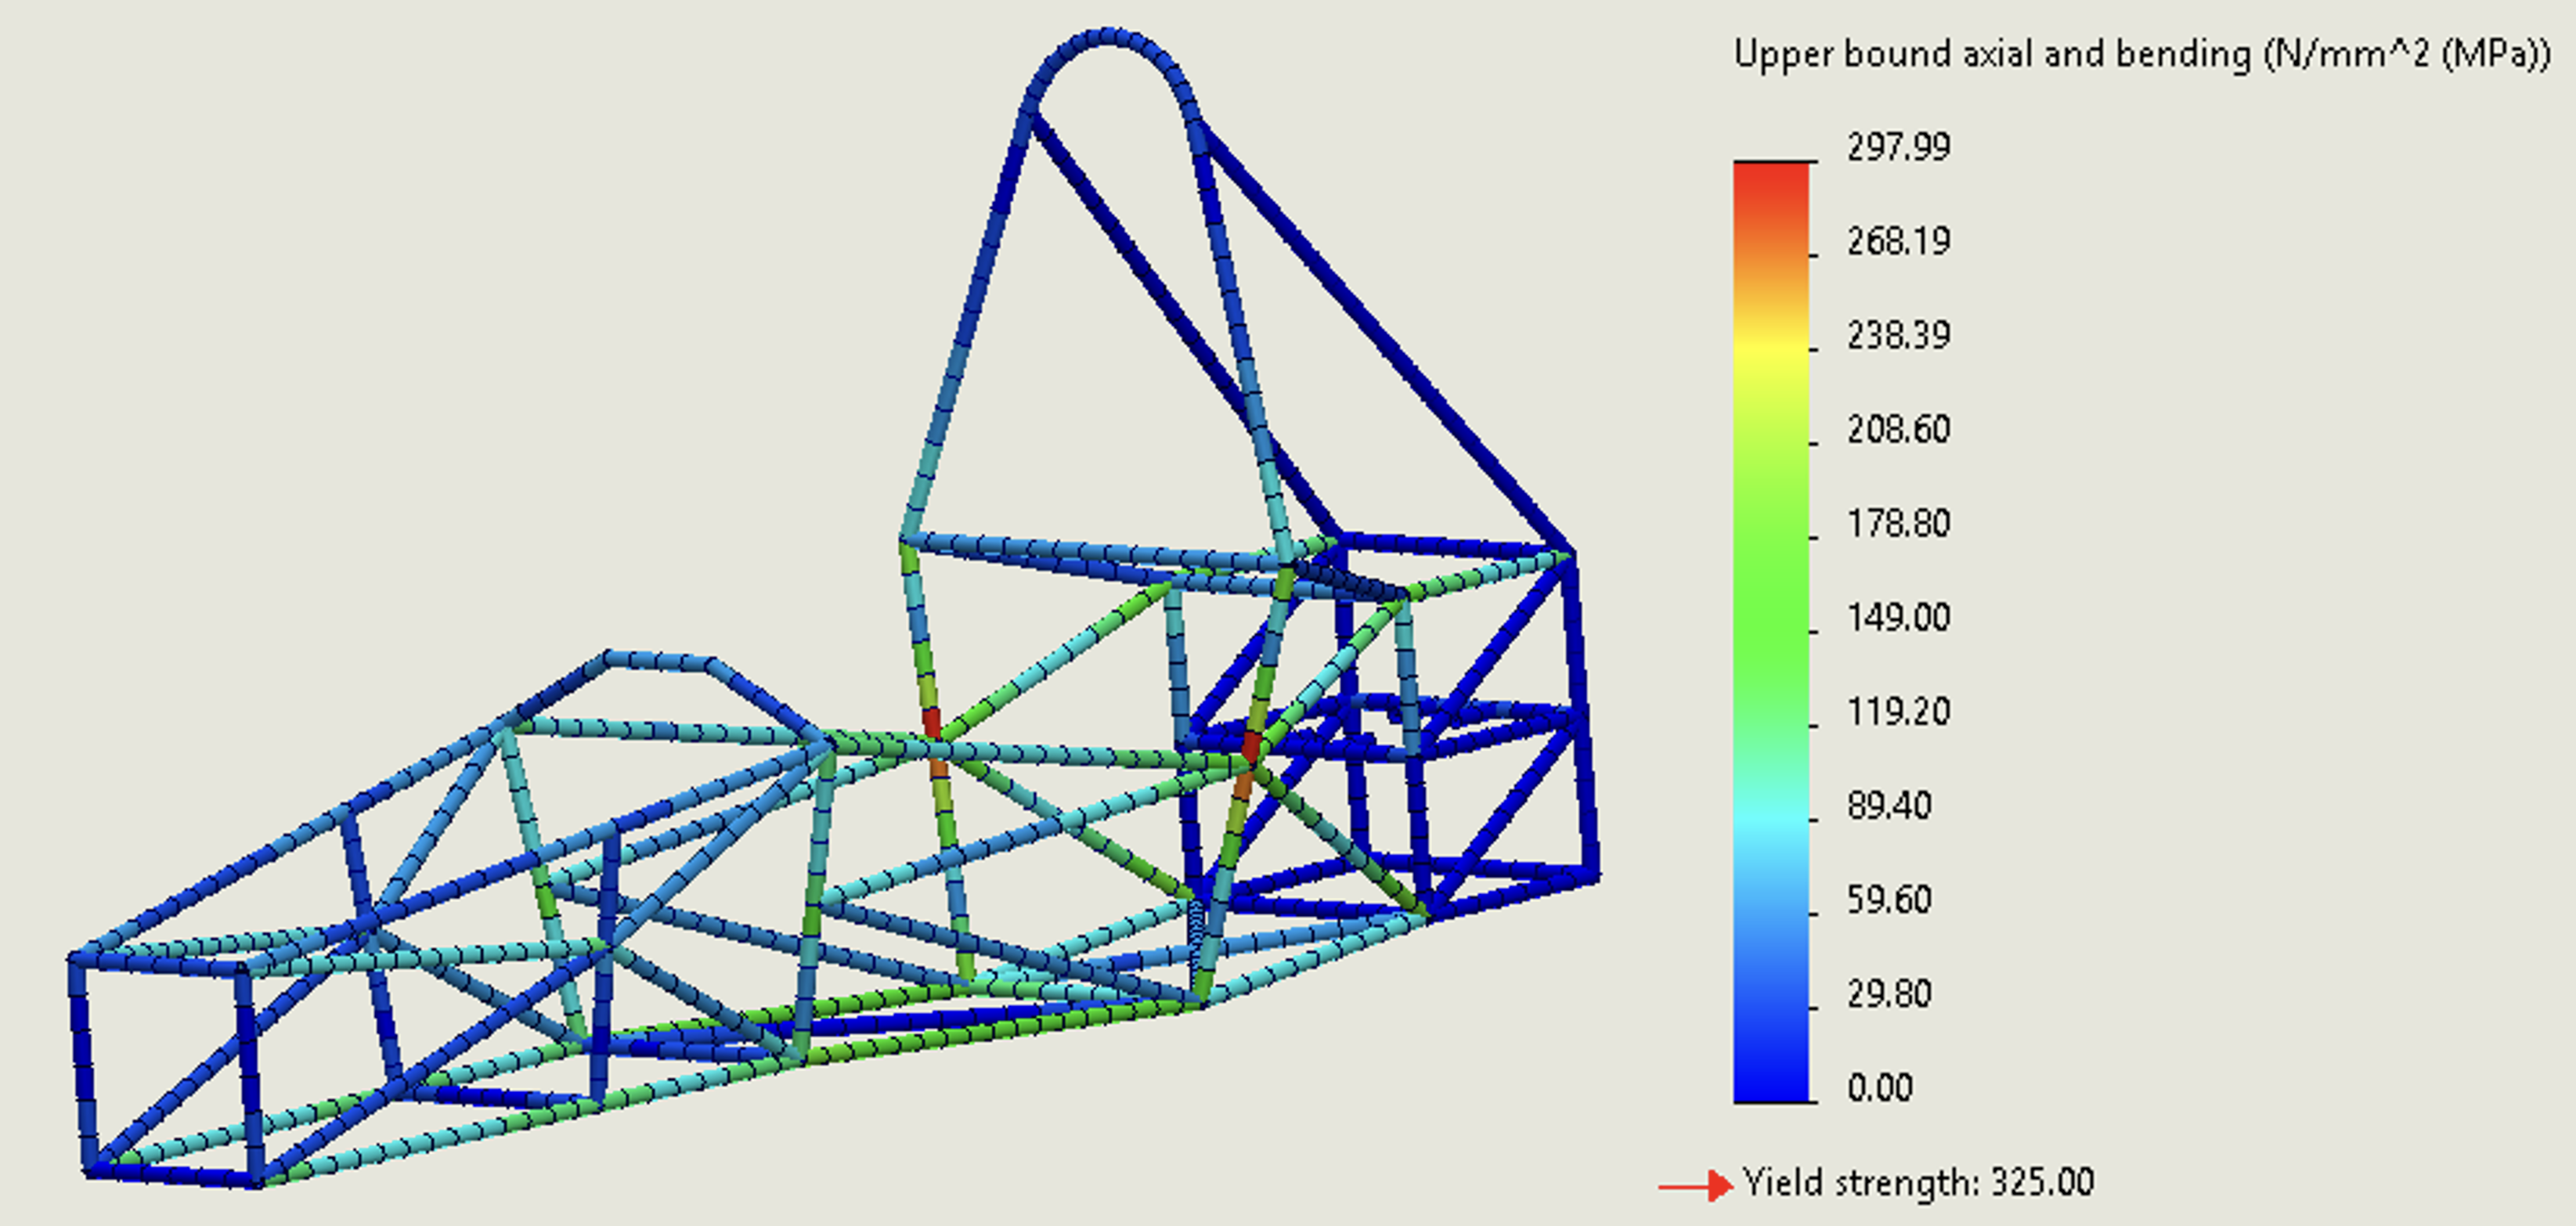
\includegraphics[width=0.78\textwidth]{../TobyMcConnell/Engineering/Images/badfrontfinal.png}
    \caption{Front Impact Stress Distribution Without Support Bars}
    \label{fig:fail_front_impact_stress}
\end{figure}

\begin{figure}[htbp]
    \centering
    \begin{subfigure}{0.49\textwidth}
        \centering
        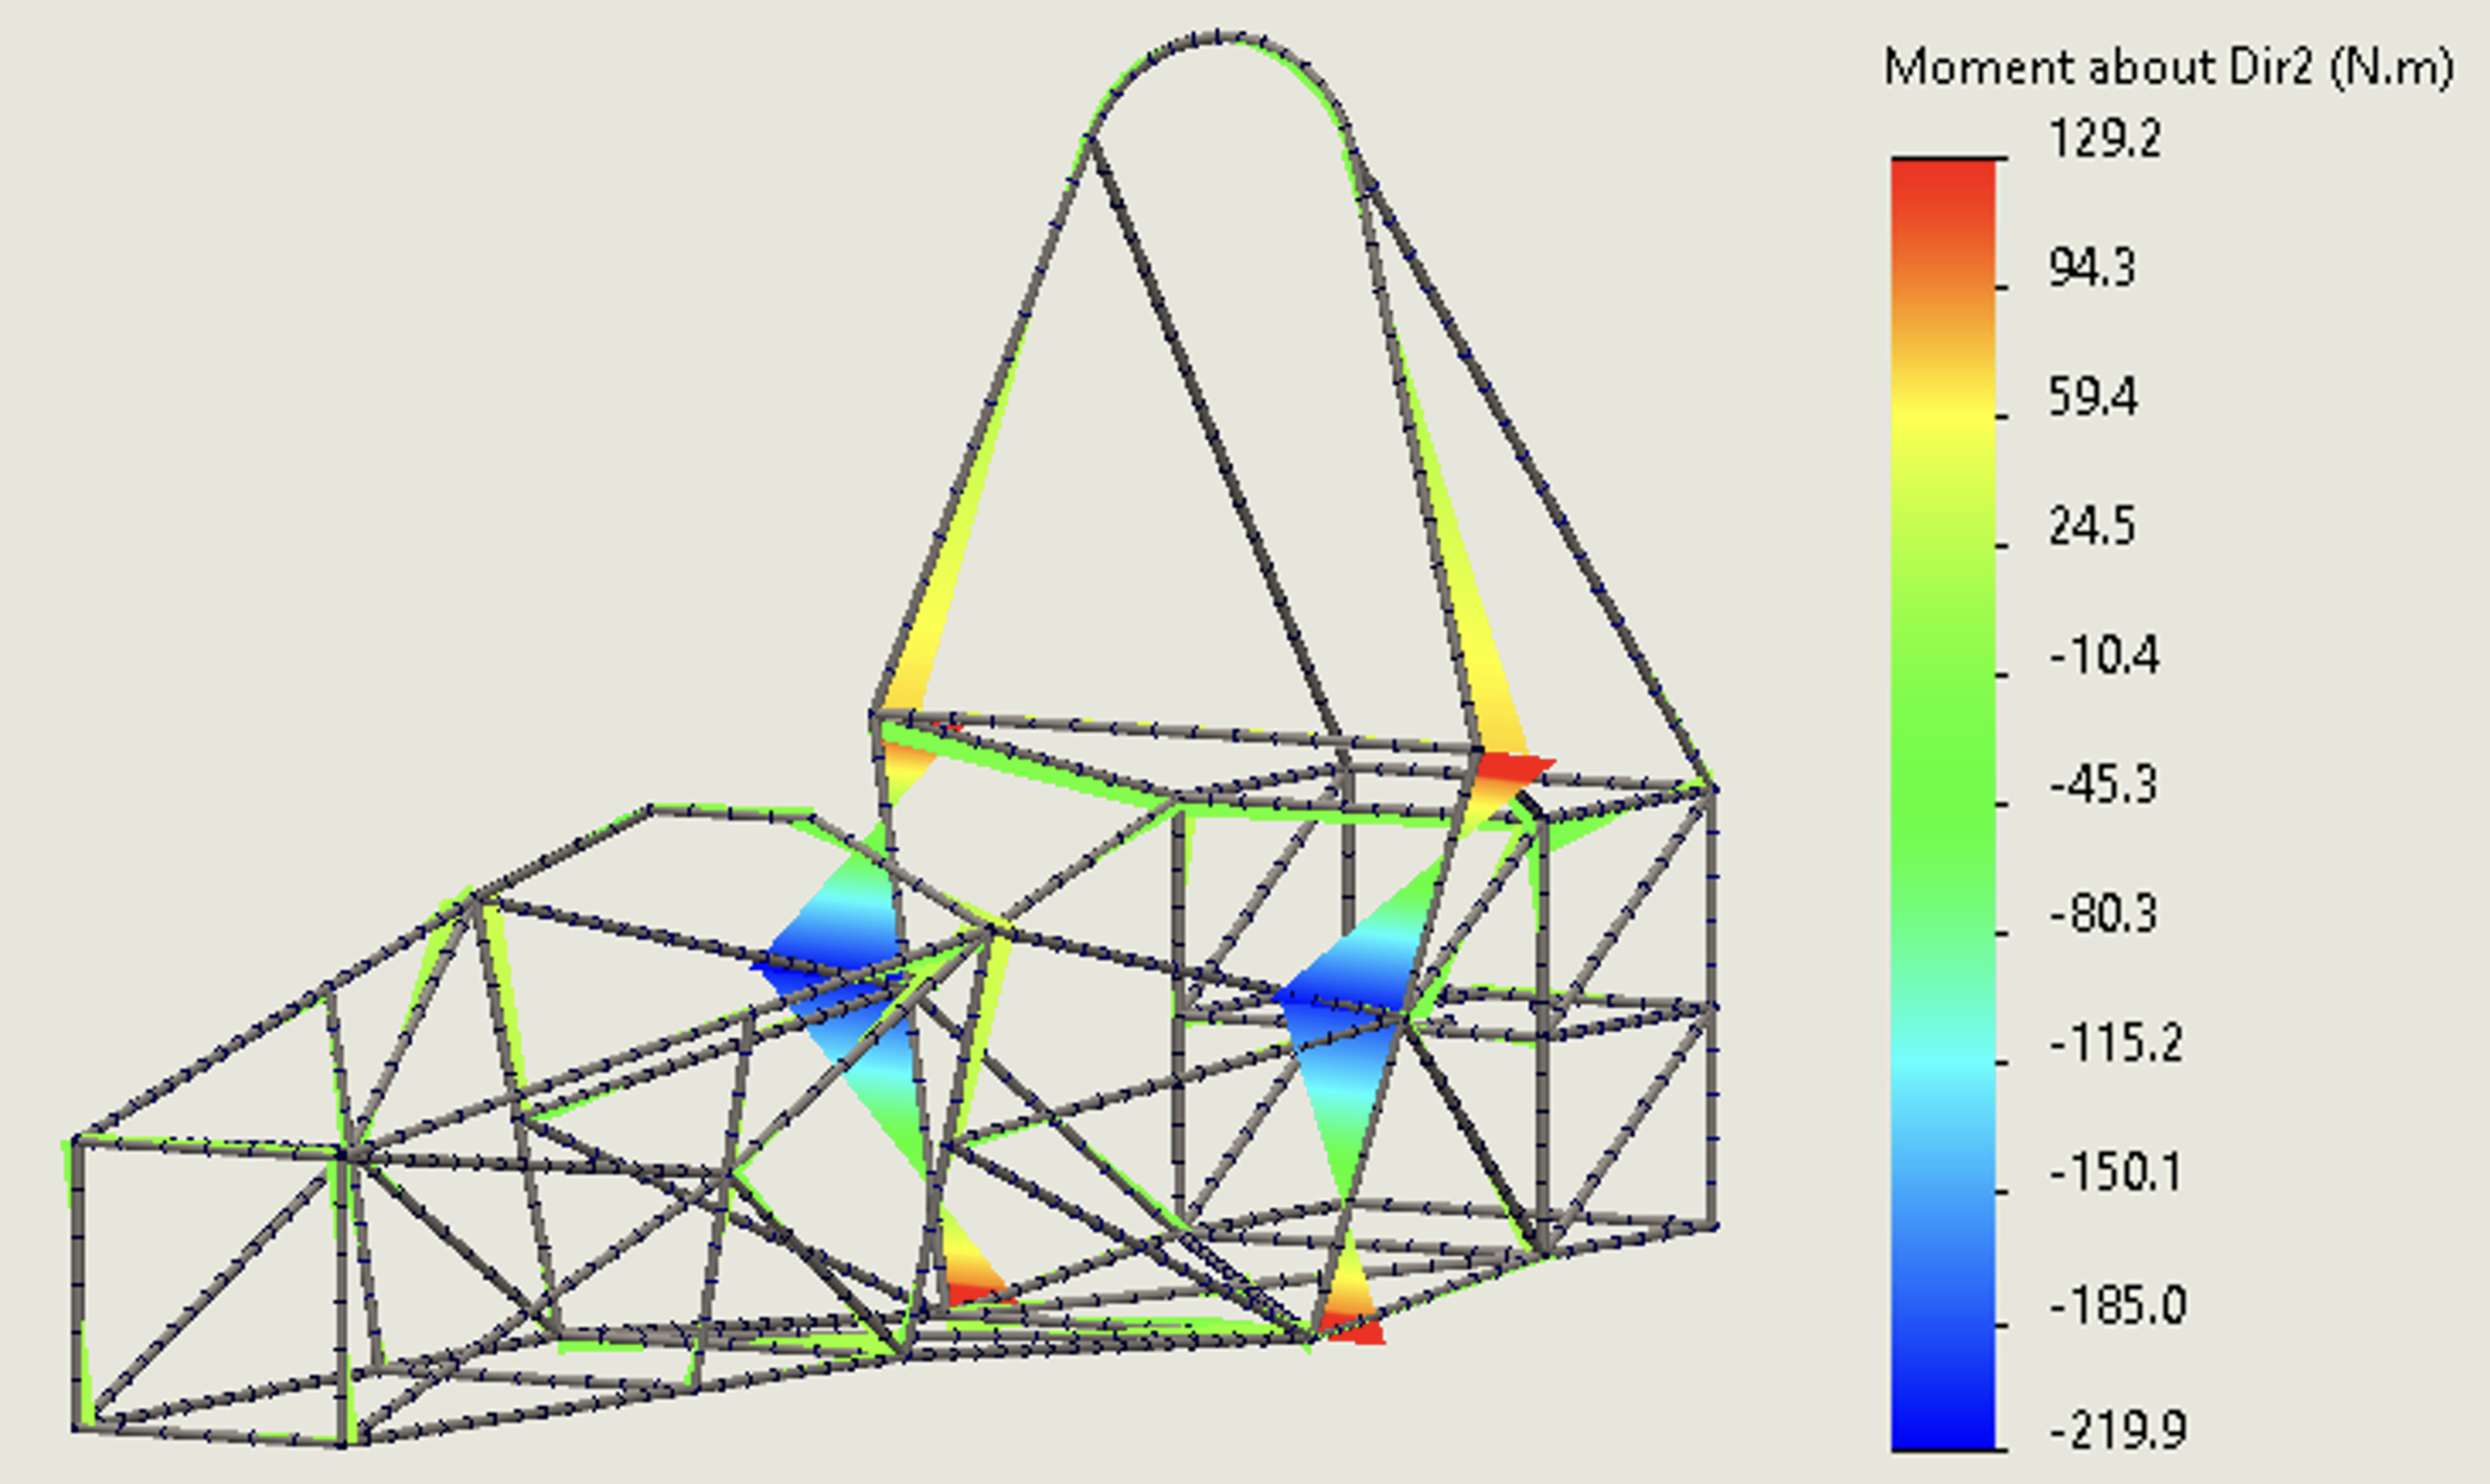
\includegraphics[width=\linewidth]{Images/momentfinal.png}
        \caption{Moment Distribution in Front Impact}
        \label{fig:moment_front_impact}
    \end{subfigure}
    \hfill
    \begin{subfigure}{0.5\textwidth}
        \centering
        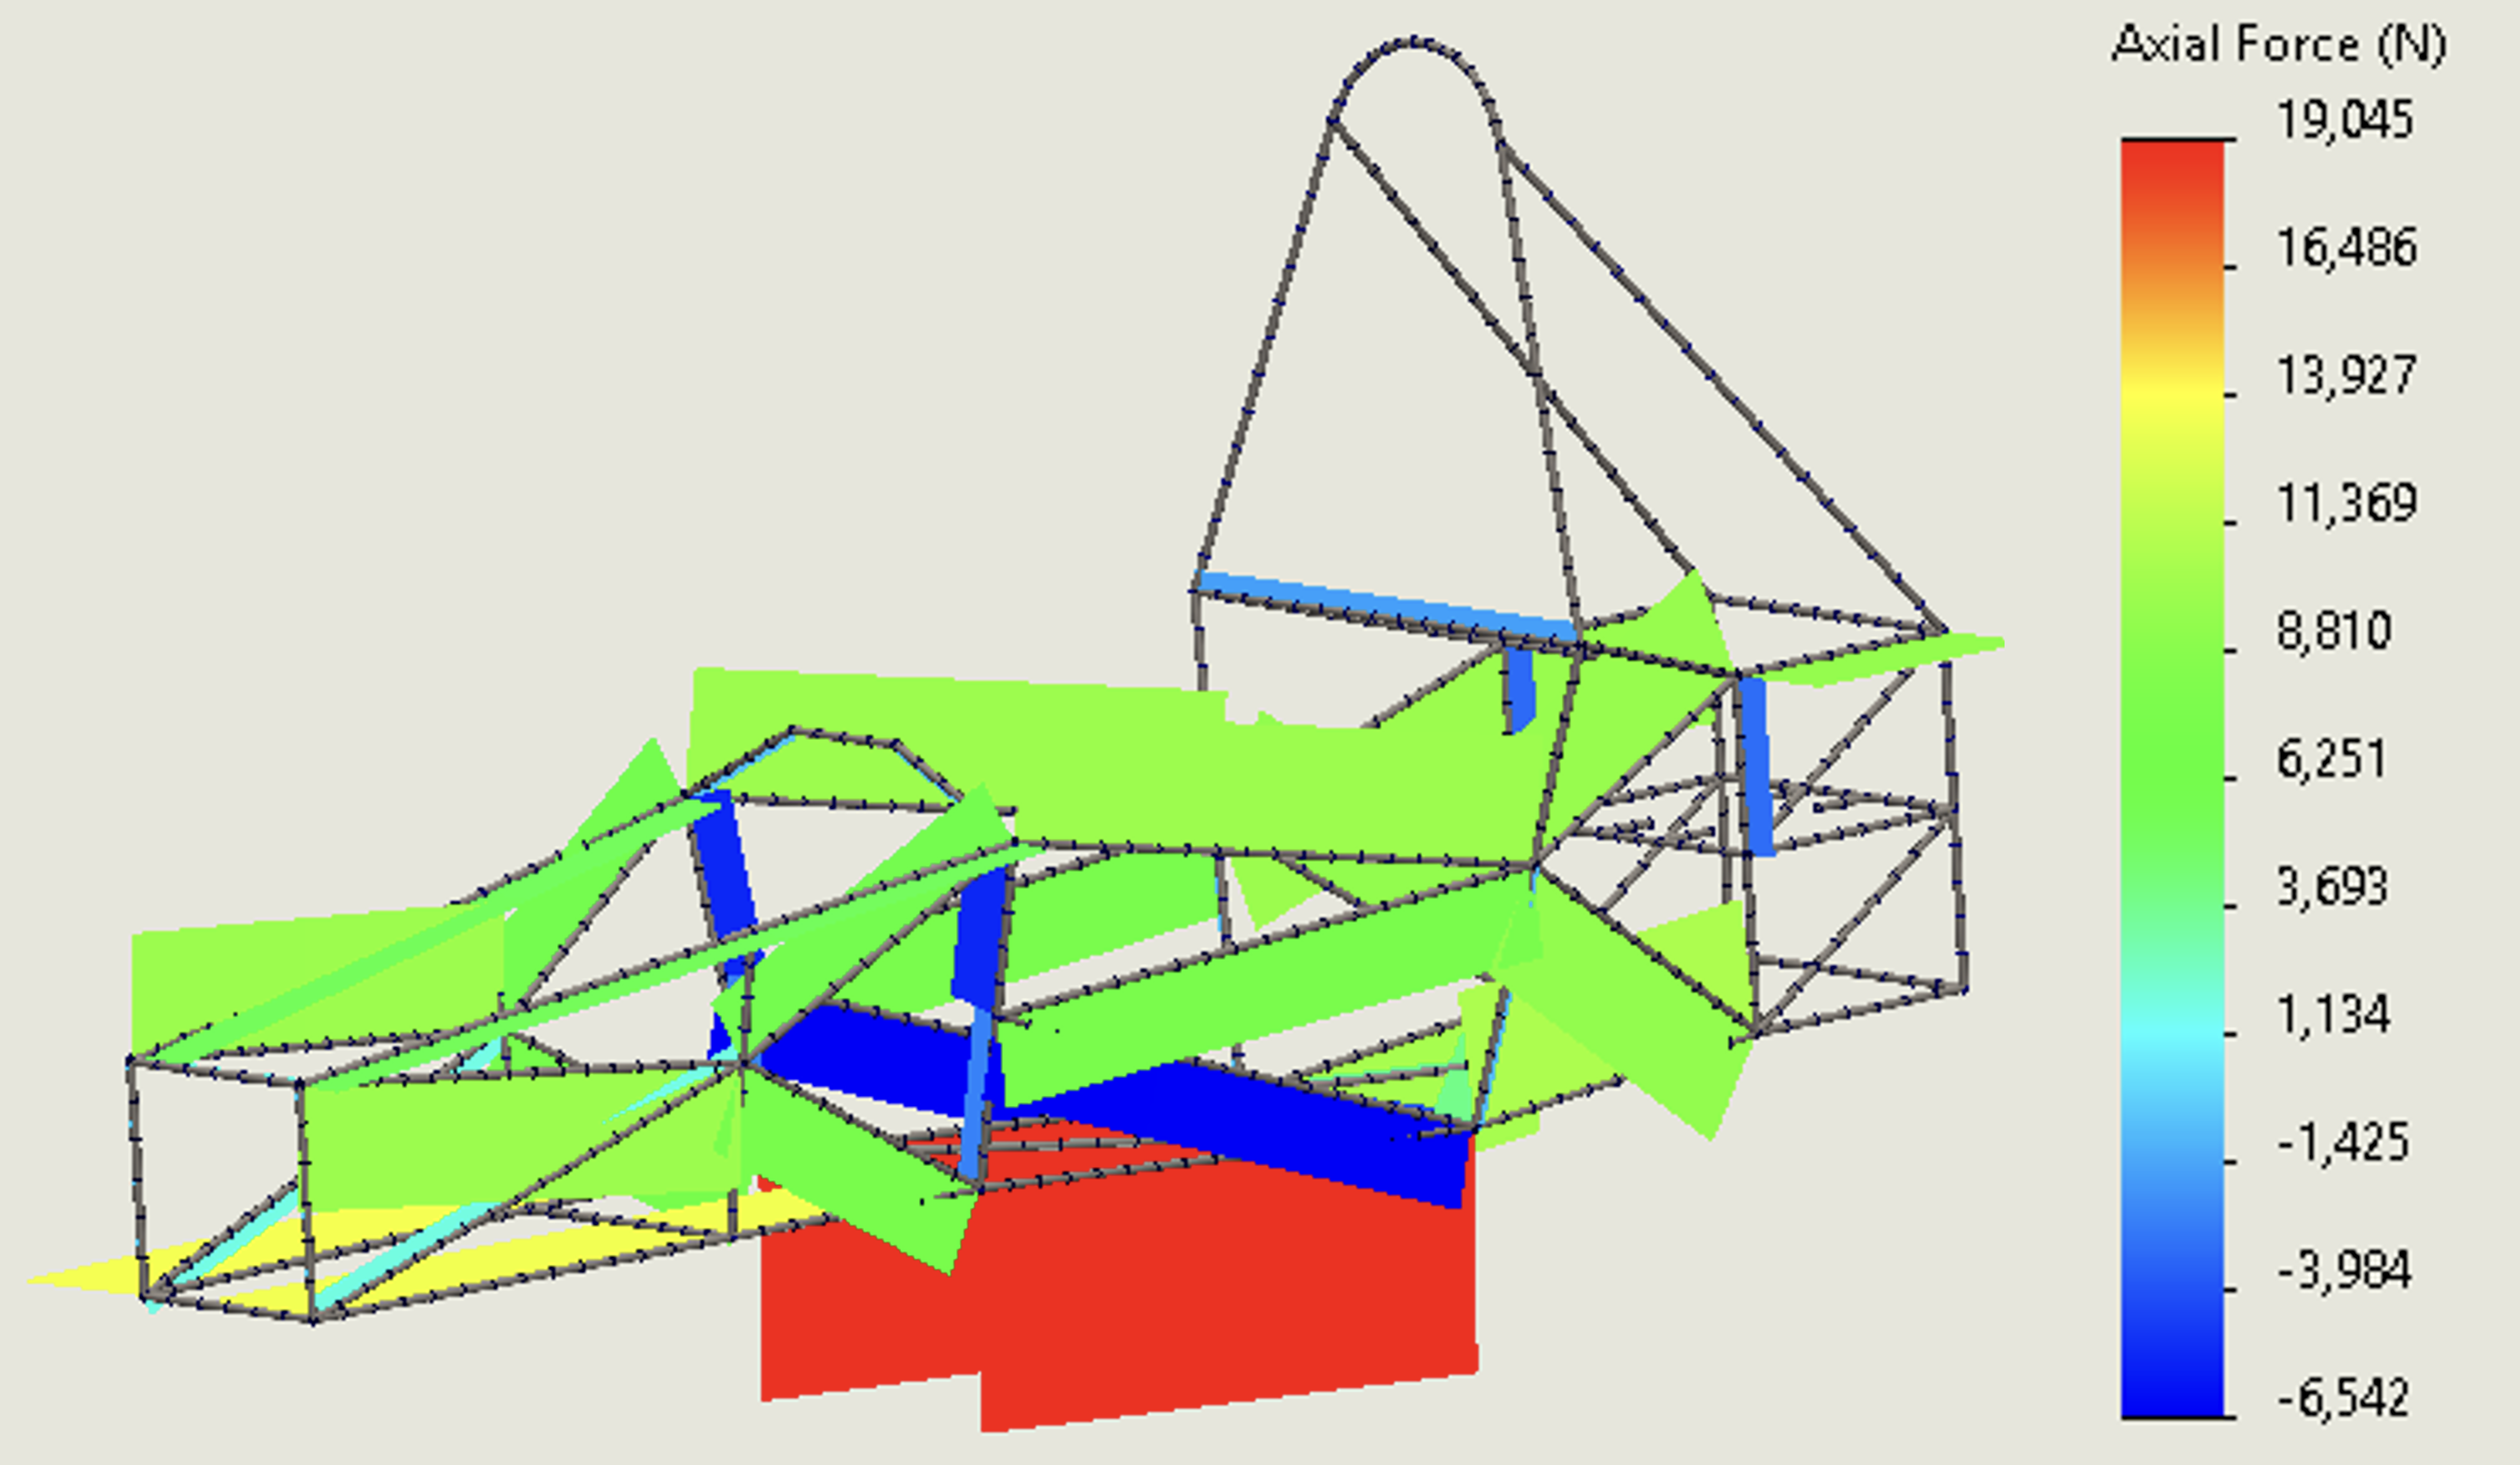
\includegraphics[width=\linewidth]{Images/compressionfinal.png}
        \caption{Axial Force Distribution in Front Impact}
        \label{fig:compression_front_impact}
    \end{subfigure}
    %\caption{Two figures side by side}
    %\label{fig:both}
\end{figure}


This analysis can be used to show the process we went through in verifying all the bars in the structure were necessary for a safe chassis capable of protecting the driver in all impact scenarios by justifying the two bars at the top of the cockpit.

The simulation, without the support bars, showed that several members experienced high stresses, with the maximum (298MPa) occurring at a joint where four structural members converge in the side impact structure (fig. \ref{fig:fail_front_impact_stress}). This stress was over our safety value ($0.9*325=292.5MPa$) but, as stated earlier, a small risk of yield during worst case crash scenario was acceptable. At this level of stress at such a complex joint, weld failure was a concern. Additionally, welded joints in this region may experience reduced strength due to the heat-affected zone created during fabrication. Looking into the FEA deeper we found the stress was mainly caused by a large moment of 219.9Nm at that mount (fig. \ref{fig:moment_front_impact}). Moments are more dangerous because they create a "prying" action that concentrates the entire load as a peak stress at the very edge of the weld, whereas axial forces distribute the load uniformly across the entire weld surface. With the total weld stress $>0.75* \text{failure stress}$ (see \ref{tab:weld_vs_tube}), a gusset to increase the throat. Therefore weld strength or a chassis structural change to the chassis would be required, making a gusset the cheaper and easier option.

On checking the third failure mode, the axial force distribution revealed one of the bars in the side impact structure had a high compressive load (6.54kN), requiring a critical buckling load calculation:
\vspace{-5pt}
\begin{align*}
\text{Second moment of area: } & I = \frac{\pi}{64}(D^4-d^4) = \frac{\pi}{64}(25^4-21^4) = 9.63 \times 10^{3}~\text{mm}^4, \\
\text{Reduced Euler load (imperfection factor 0.7): } & P = 0.7 \cdot \frac{\pi^2 E I}{(K L)^2} = 0.7 \cdot \frac{\pi^2 (200 \times 10^9)(9.63\times10^{-9})}{(1 \cdot 1.05)^2} = 12.0~\text{kN}, \\
\text{Design critical load with safety factor 0.5: } & P_{\text{critical}} = 0.5 \cdot P = 0.5 \cdot 1.20 \times 10^{4} = 6.0 \times 10^{3}~\text{N} = 6.0~\text{kN}, \\
\text{Comparison with applied load: } & P_{\text{critical}} = 6.0~\text{kN} < 6.5~\text{kN}
\end{align*}

These compression safety factors used are strict but in combination with the high yield risk, and potential weld failure (even with gusset, risk of manufacturing errors only increase) the configuration was not sufficiently robust. This verified the need for additional support bars which FEA showed yielded massive improvements: Max stress is now 165MPa and is distributed across a bar in tension not a joint or in compression also the weld joint stress was reduced by over 60\% without gussets (fig. \ref{fig:success_front_impact_stress}). This modification increased the chassis mass by approximately 1.45 kg (a 3.7\% increase), but it remained below the 45kg limit and improved driver safety justified the design trade-off.

\begin{figure}[h]
    \centering
    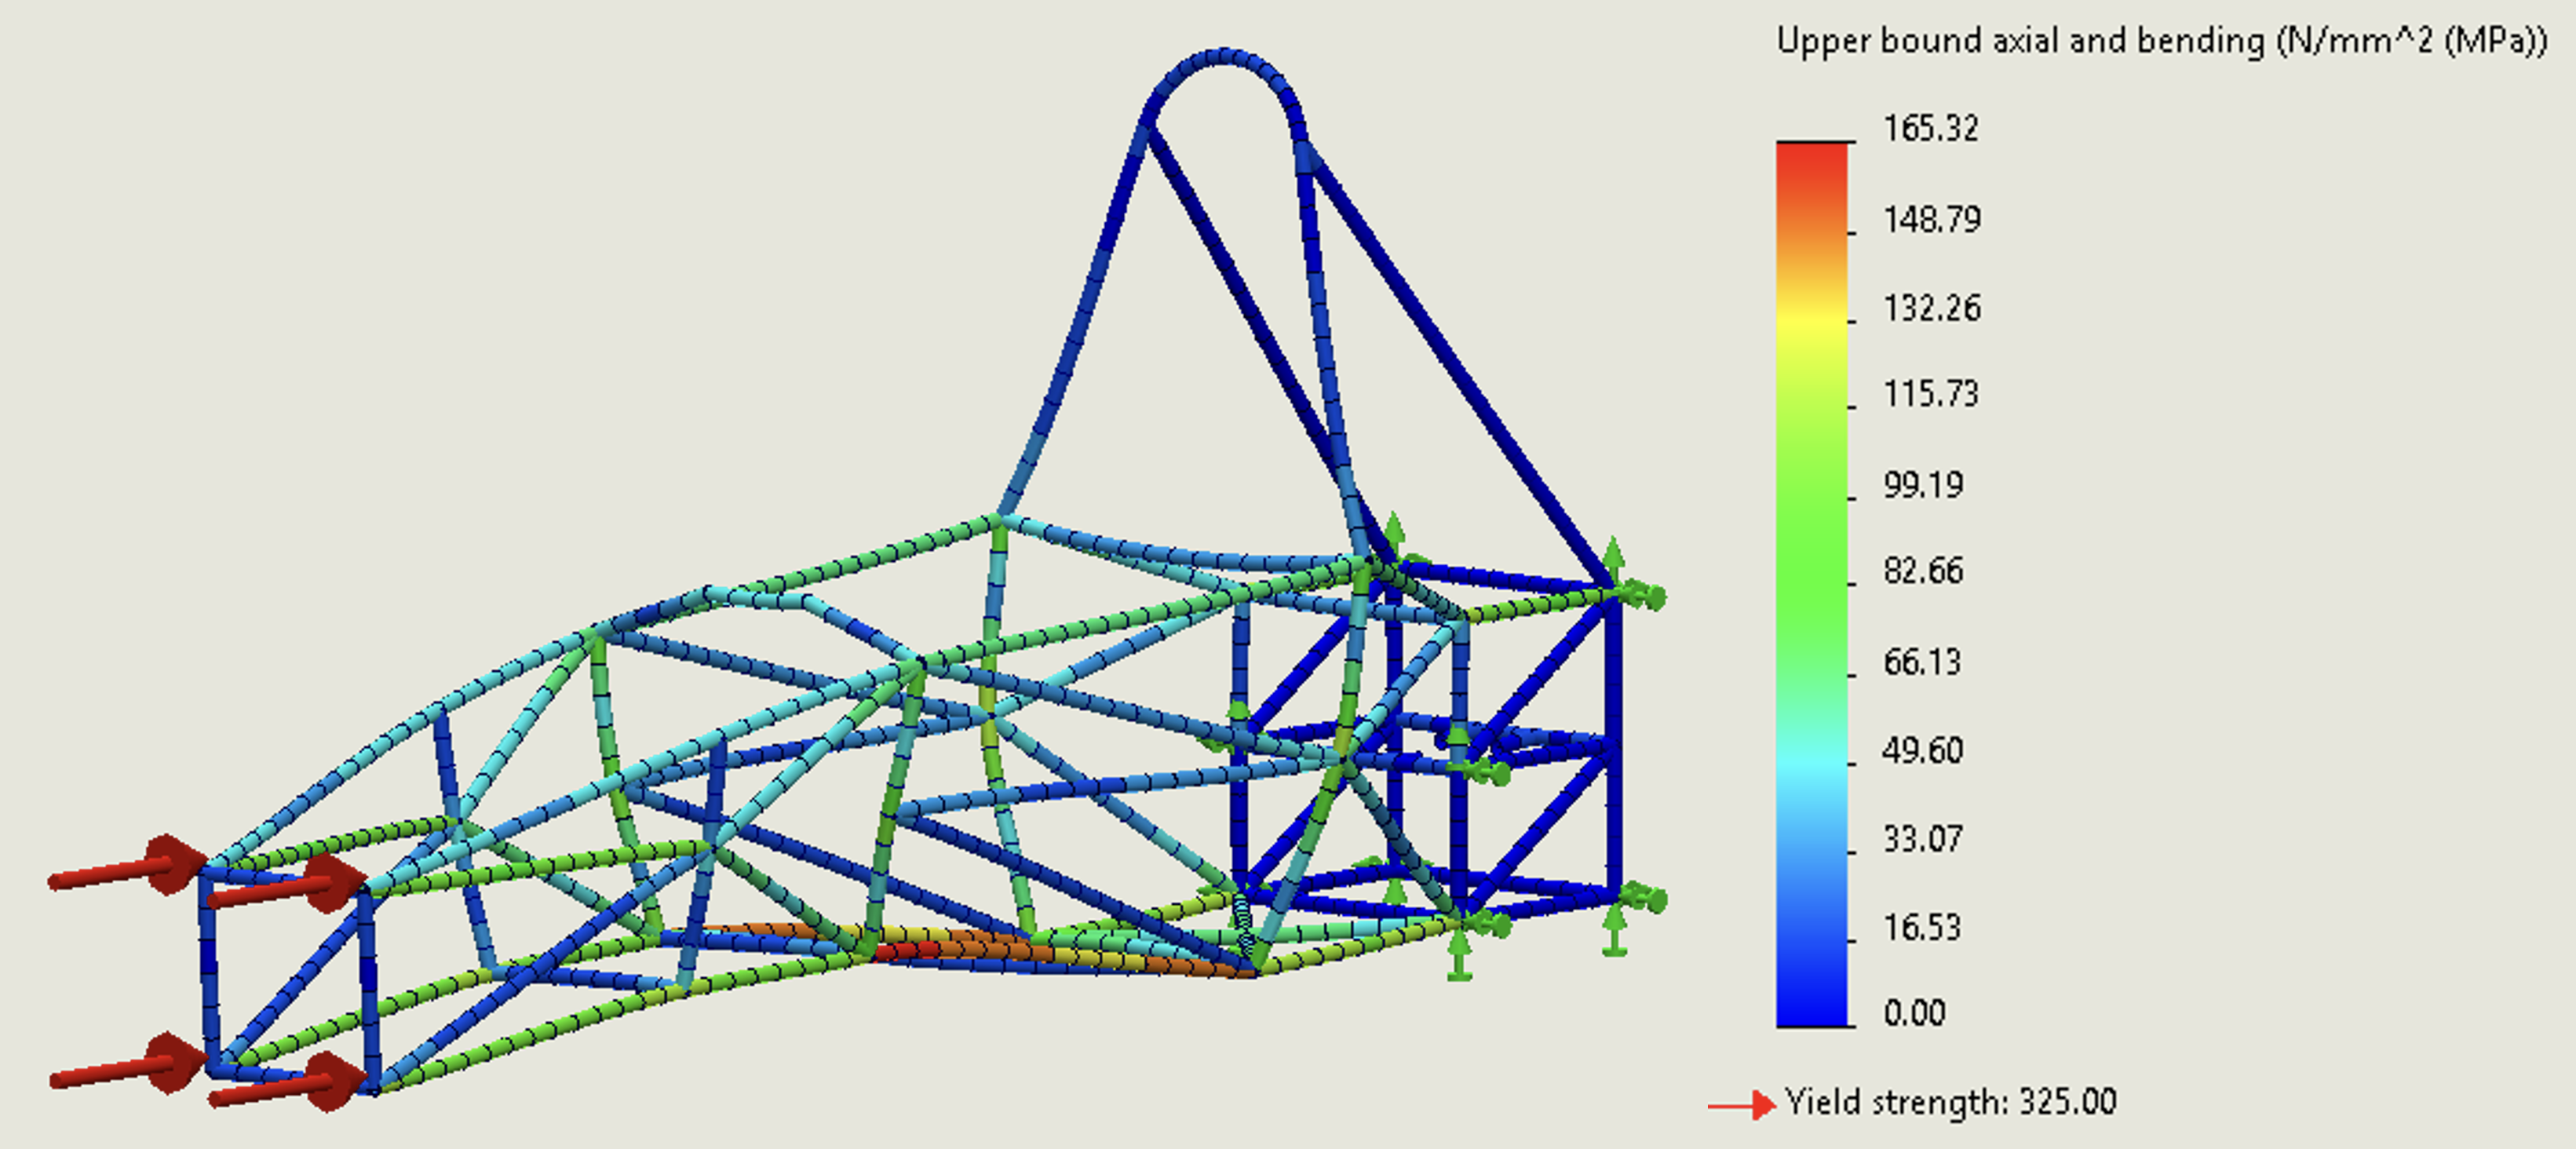
\includegraphics[width=0.82\textwidth]{../TobyMcConnell/Engineering/Images/frontfinal.png}
    \caption{Successful Front Impact Stress Distribution (Displacement Scale 30:1)}
    \label{fig:success_front_impact_stress}
\end{figure}

This method of analysis was carried out on every bar not critical for architecture or mandated by the FS regulations to ensure there were no unnecessary bars in the final chassis.

\subsection{Rear and Side Impact Simulations}

Rear and side impact simulations were also performed. Since we are only using our car in an acceleration events there is no risk of collisions with other cars (e.g., T-bone crash). Therefore the forces are estimated based on a crash where the car spins of track and hits a safety barrier by its side or rear first. Energy dissipation during the spin results in significantly lower impact speed than a direct frontal collision. Rear and side impact forces of 40kN and 60kN respectively were used on this basis. Figures \ref{fig:rear_impact} and \ref{fig:side_impact} show the distribution of forces (red arrows) and fixed joints (points marked green) as well as the results of these simulations.

\begin{figure}[htbp]
    \centering
    \begin{subfigure}{0.5\textwidth}
        \centering
        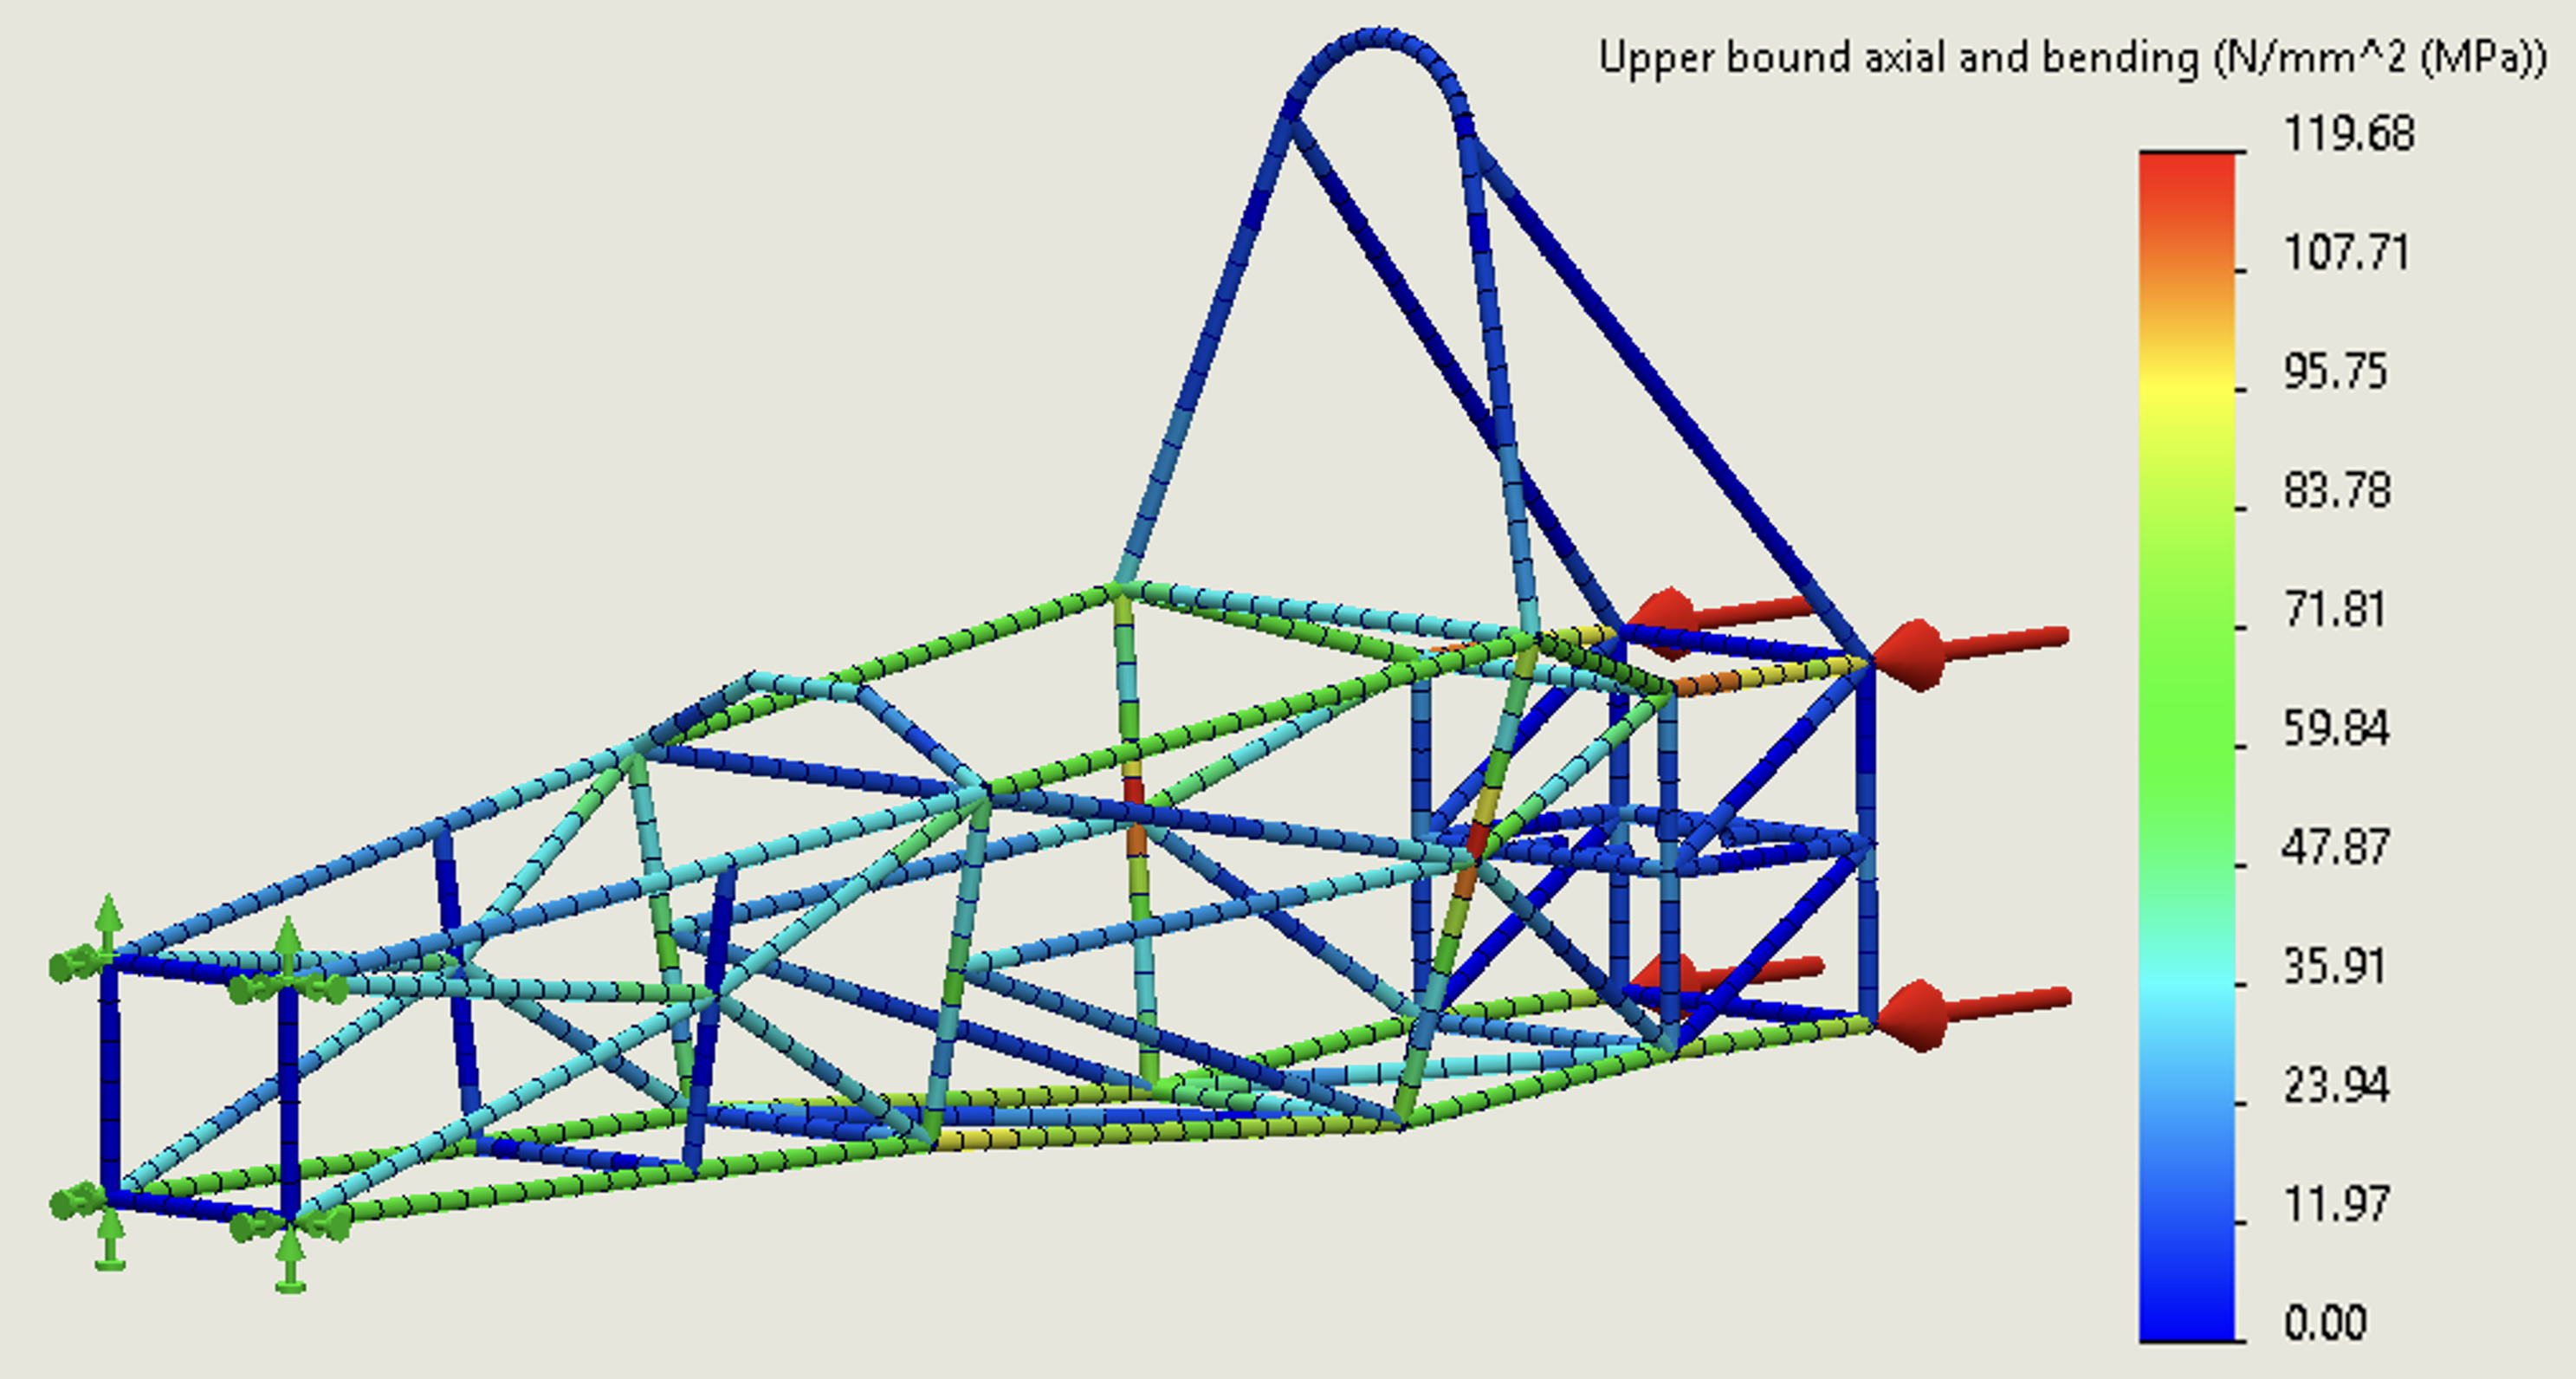
\includegraphics[width=\linewidth]{Images/reversefinal.png}
        \caption{Rear Impact: Force = 40kN}
        \label{fig:rear_impact}
    \end{subfigure}
    \hfill
    \begin{subfigure}{0.49\textwidth}
        \centering
        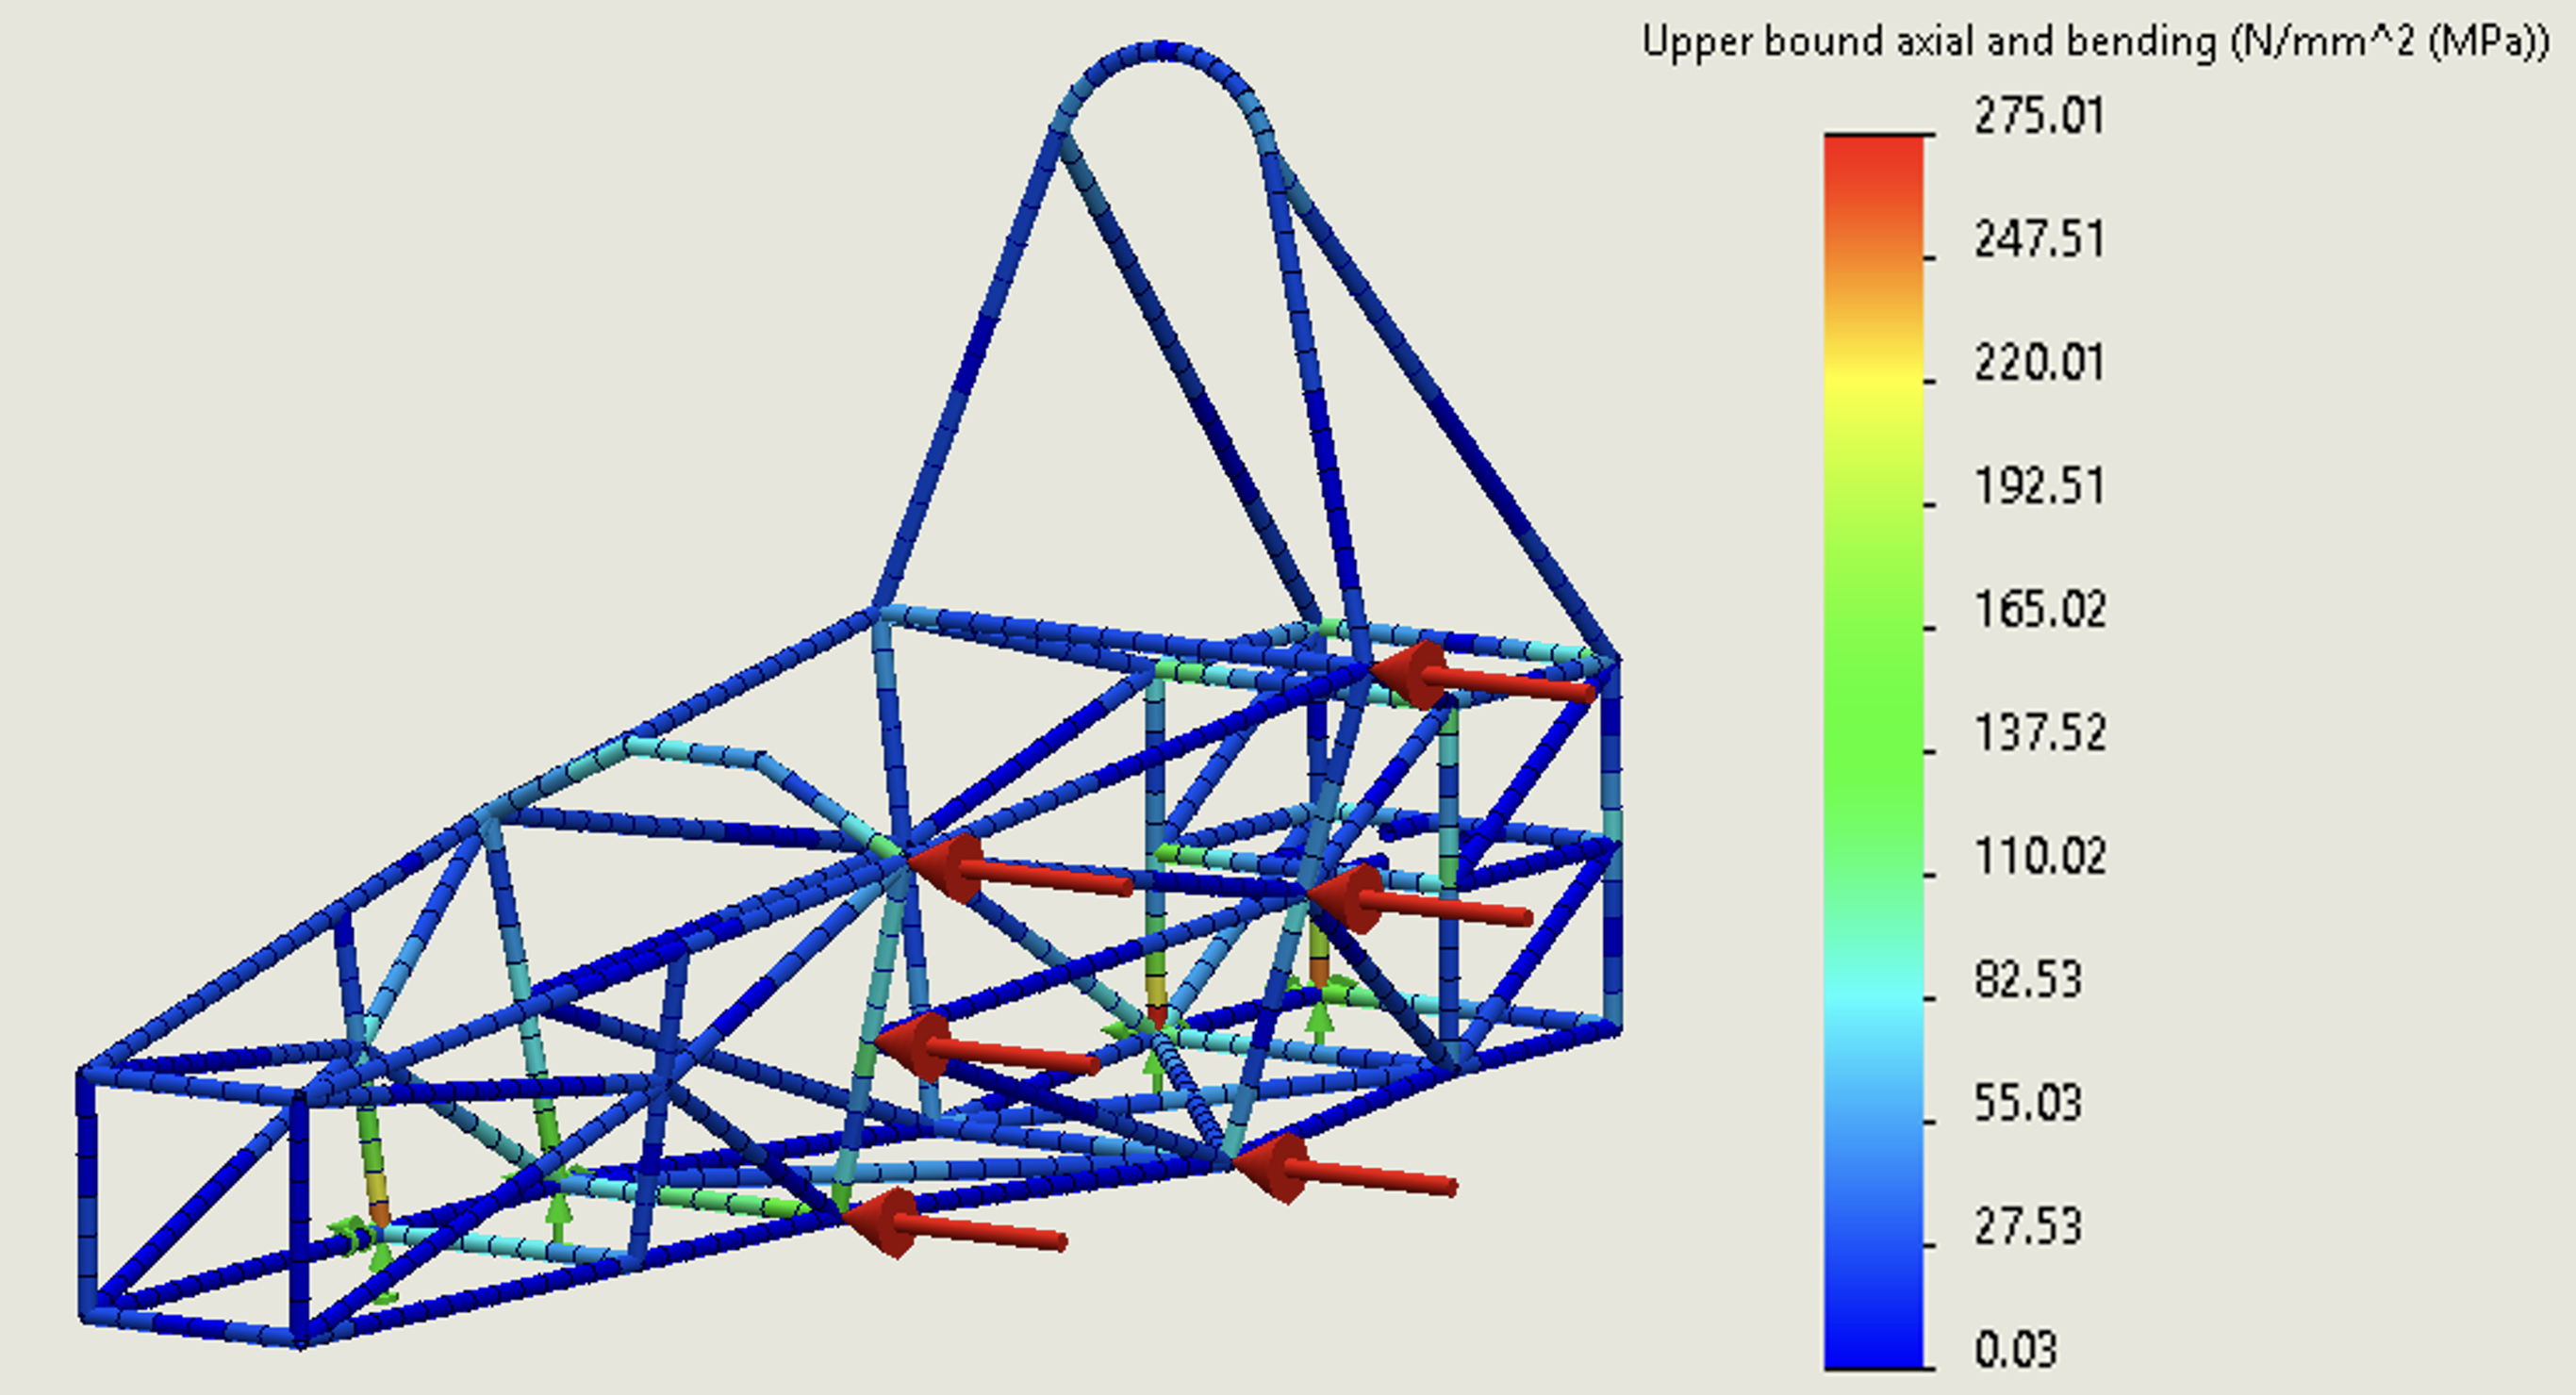
\includegraphics[width=\linewidth]{Images/sidefinal.png}
        \caption{Side Impact: Force = 60kN}
        \label{fig:side_impact}
    \end{subfigure}
    %\caption{Two figures side by side}
    %\label{fig:both}
\end{figure}
\vspace{-5pt}

The only region with elevated stress occurred near the suspension mounting points, where structural reinforcements are already present to support wheel loads. This stress is within the limits ($0.9 * 325 > 275$). A small yield in a side impact situation is acceptable as it very unlikely in the acceleration event and not in any of the key safety areas so the driver is safe regardless. These simulations also showed no bars under high compression or welds under high moments or total stress thus ensuring the driver is safe and the chassis is optimised for all operational and crash scenarios.

\section{Compliance and Conclusion}

\begin{figure}[h]
    \centering
    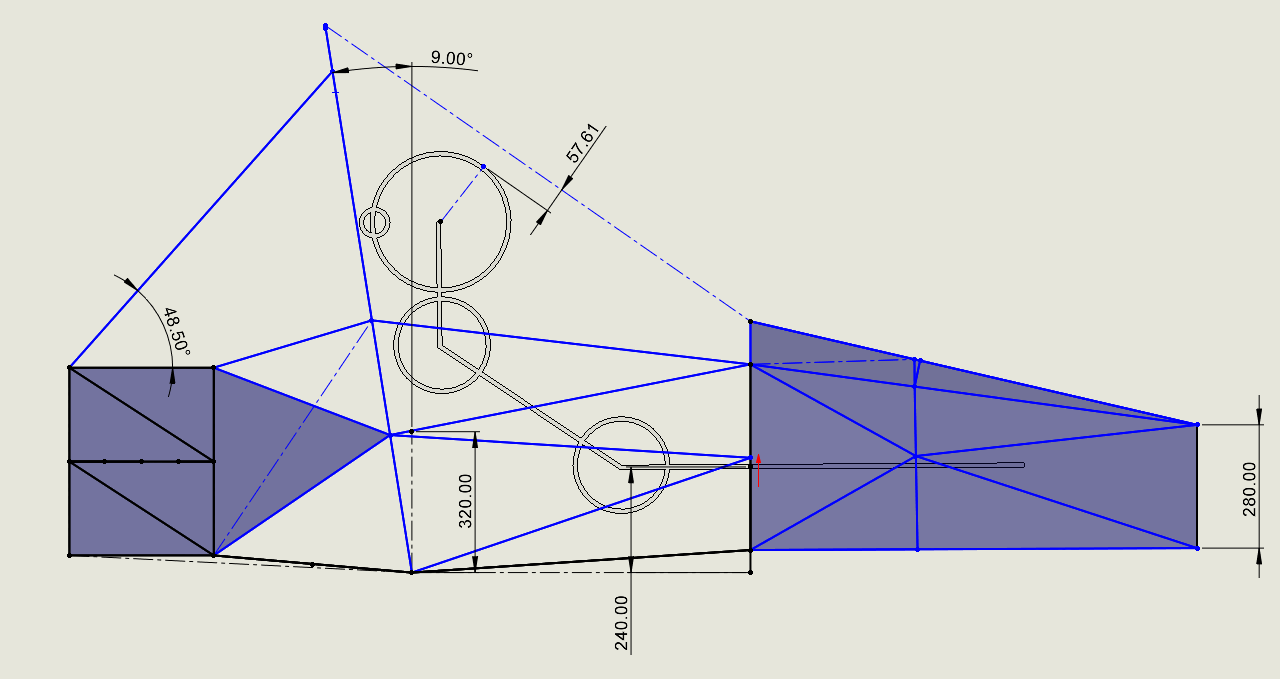
\includegraphics[width=0.7\textwidth]{../TobyMcConnell/Engineering/Images/compliance.png}
    \caption{Compliance}
    \label{fig:Compliance}
\end{figure}

The final design complies with the required regulations, including angle of main roll hoop support, helmet clearance, main roll hoop angle, side impact structure, IA plate (IAP) size (square with length in figure), fully triangulated structure (Figure \ref{fig:Compliance}), as well as cockpit opening dimensions, front bulkhead/leg cross-section, steering wheel clearance, seatbelt mount positioning (at main roll hoop cross-bar intersection), pedal box clearance, and packaging of all CAD verified major components. This gives us a verified, cost-effective structural foundation to build the rest of the vehicle around. Further possible work should focus on the integration of lightweight composite bodyworks, verified powertrain mounting structures and targeted aerodynamic packages to further reduce drag, alongside a physical testing phase to validate FEA predictions.
\vspace{+5pt}
\compactbib
% --- END INLINE: TobyMcConnell/Engineering/toby_body.tex ---
\end{refsection}

\begin{refsection}
\graphicspath{{../MichaelZiyangXing/}}
% -----------------------------------------------------------------------------
% Engineering chapter section for the Formula Student acceleration vehicle.
% Designed for inclusion in latex/CombinedFinal/main_single_file.tex.
% Requires the master file to load: styling.sty, biblatex, tabularx, siunitx,
% graphicx, subcaption, float and the references_wheel_assembly.bib file.
% -----------------------------------------------------------------------------
\providecommand{\figbox}[2]{\begin{figure}[H]\centering\fbox{\parbox[c][#1][c]{0.92\linewidth}{\centering #2}}\caption{#2}\end{figure}}

\chapterauthor{Wheel Assembly Design}{Ziyang Xing}
\vspace{-25px}
%\contribution{This chapter presents the author's individual engineering contribution to the Formula Student acceleration vehicle: the wheel assembly, suspension, steering and braking design, with detailed focus on the rear multi-link suspension, anti-squat/toe strategy, and single inboard brake acting on the limited-slip differential.}
\label{chap:wheel_assembly_design}

\section{Wheel assembly design scope and key terminology}

\subsection{Scope of this chapter}
This chapter presents the wheel-assembly design for the acceleration-only Formula Student UK vehicle. The previous chapter establishes the vehicle-level event objective; this chapter explains how the suspension, steering and braking choices support that objective at the wheel-assembly level. The front suspension, steering system and front brakes are included because they are required for a complete and rule-compliant vehicle, but the main engineering contribution is the rear wheel assembly. The rear design combines multi-link kinematics, a tunable anti-squat target, dynamic rear toe control, and a single inboard brake acting on the limited-slip differential (LSD).

The vehicle is not intended to be a balanced skidpad, autocross and endurance car. Its useful dynamic case is launch and short straight-line acceleration. The rear suspension can therefore be biased towards rear traction, ride-height control, low scrub and wheel-end mass reduction. The chosen wheel package is the OZ Racing Formula Student Hybrid Carbon CL \SI{10}{in} wheel and Hoosier 18.0 x 6.0-10 Formula Student slick tyre. OZ lists the 7 x 10 in hybrid carbon wheel at approximately \SI{1.35}{kg}, while Hoosier lists the 18.0 x 6.0-10 slick at approximately \SI{9}{lb} \parencite{zxOZCarbon10,zxHoosierSpecs}. These light components make the remaining upright, brake and link mass important to the corner-mass budget.

\subsection{Definitions used in the design argument}
\textit{Toe angle} is the plan-view angle between the wheel and the vehicle centreline. \textit{Toe-in} points the front of the wheel inwards; \textit{toe-out} points it outwards. Small rear toe-in can improve straight-line stability, while zero toe reduces tyre scrub and power loss in straight running \parencite{zxSuspensionSecretsToe}. \textit{Camber} is the front-view wheel inclination relative to vertical. It is secondary for this acceleration-only design, but it must remain adjustable to compensate for manufacturing and setup variation.

\textit{Squat} is the rear suspension compression caused by acceleration load transfer. \textit{Anti-squat} is a geometric force-path effect that resists this compression. The driven tyre force passes through the suspension links; if the side-view force line is inclined, a vertical jacking component is generated. Anti-squat is therefore part of the same suspension-kinematics problem as bump steer, wheel-centre path and compliance steer \parencite{zxMilliken1995,zxDixon2009}. \textit{Bump steer} is toe change during wheel bump or rebound. \textit{Unsprung mass} is mass that moves with the wheel, including wheel, tyre, hub, upright and outboard brake hardware.

%\figbox{26mm}{Terminology schematic placeholder: plan-view toe, front-view camber, side-view squat/anti-squat force path, and inboard versus outboard brake location.}
\begin{figure}[H]
\centering
\begin{subfigure}[t]{0.49\linewidth}
    \centering
    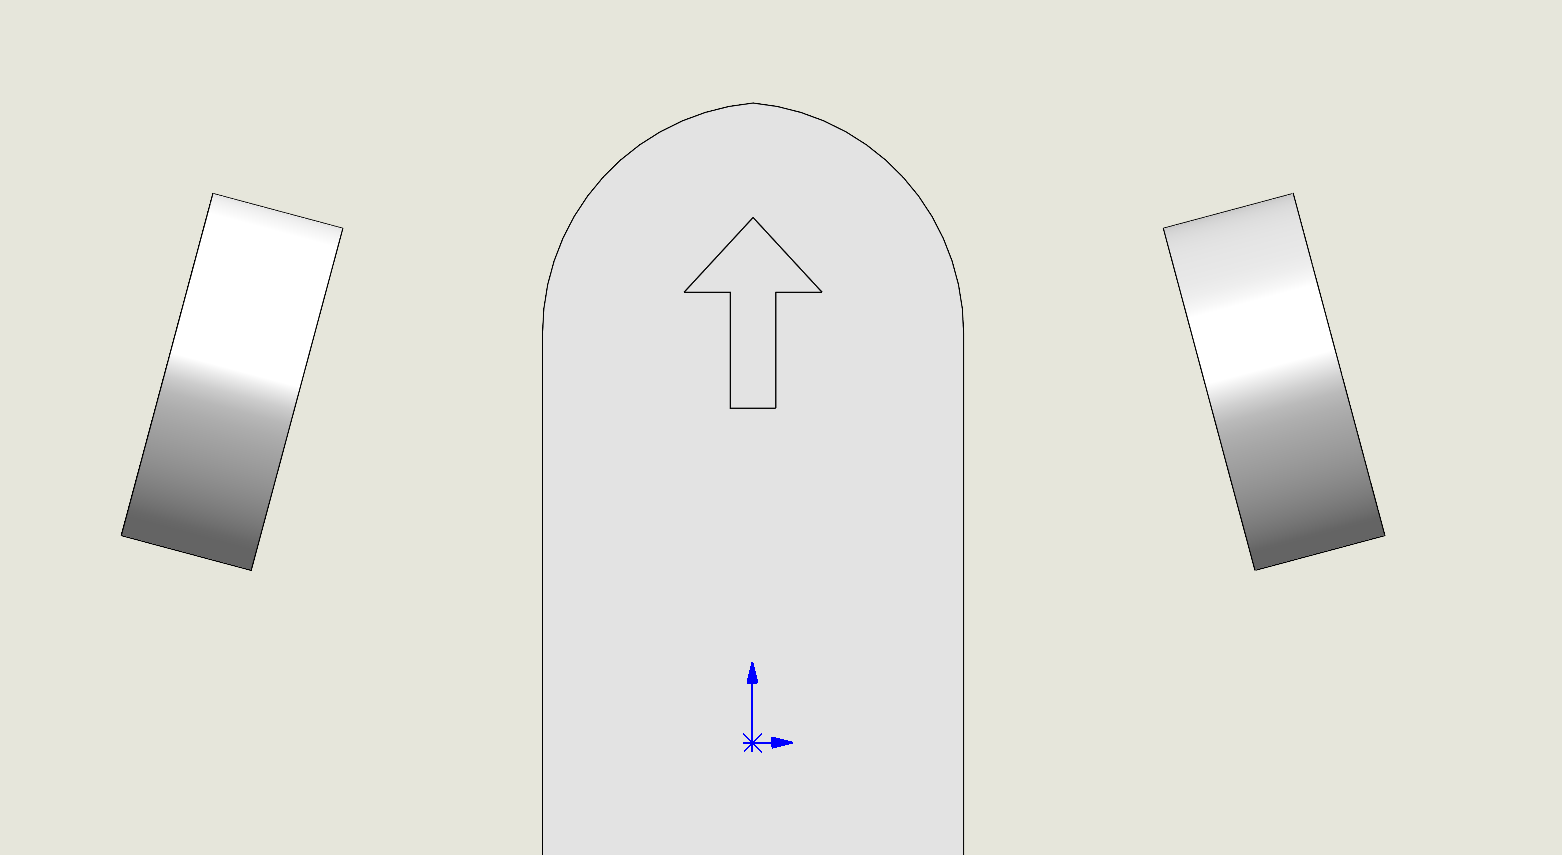
\includegraphics[width=\linewidth]{figures/Toe_Demo.png}
    \caption{Top view visual of a car with toe in.}
\end{subfigure}\hfill
\begin{subfigure}[t]{0.49\linewidth}
    \centering
    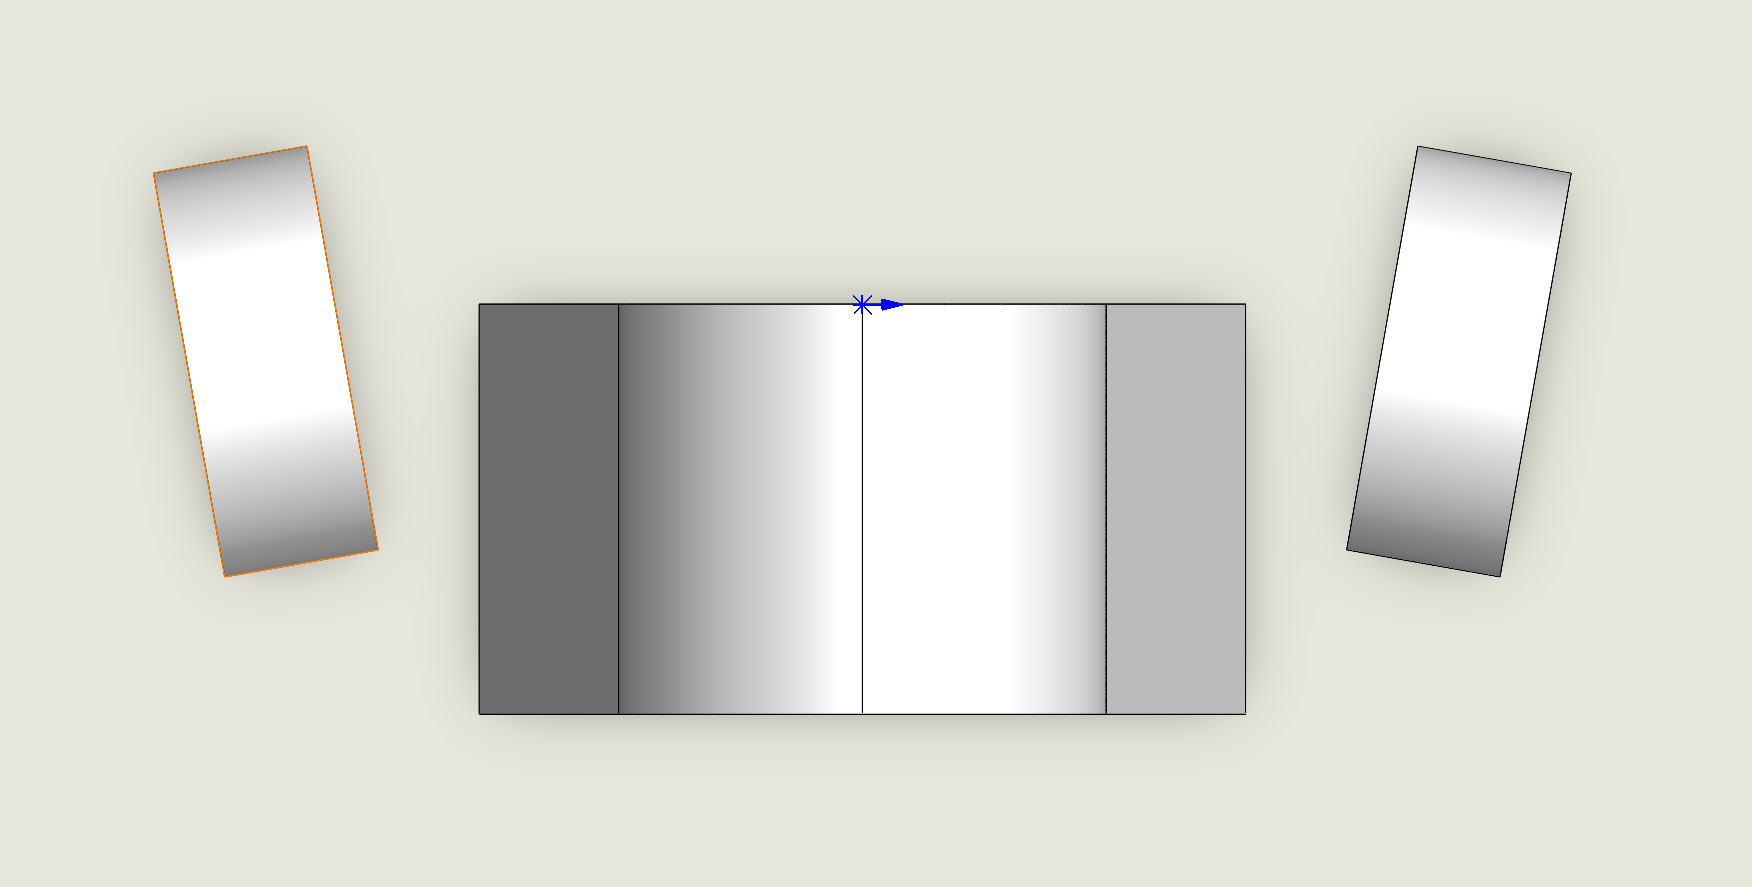
\includegraphics[width=\linewidth]{figures/Camber_Demo.png}
    \caption{Front view visual of a car with negative camber.}
\end{subfigure}
\caption{Visualizations for the suspension terminology.}
\label{fig:susp_terms_defines}
\end{figure}
\subsection{Wheel-assembly requirements}
The wheel assembly requirements were derived from rear traction, mass reduction, adjustability, rule compliance and subsystem integration. Table~\ref{tab:reqs_wheel} gives a concise flow-down from requirement area to design evidence. The table is intentionally compact: detailed vehicle-level acceleration targets are treated in the vehicle dynamics chapter, while this chapter concentrates on the physical wheel-assembly implications.

\begin{table}[H]
\centering
\caption{Wheel-assembly requirements used to guide the design.}
\label{tab:reqs_wheel}
\setlength{\tabcolsep}{4pt}
\begin{tabularx}{\linewidth}{|>{\raggedright\arraybackslash}p{0.24\linewidth}|>{\raggedright\arraybackslash}X|>{\raggedright\arraybackslash}X|}
\hline
\textbf{Requirement area} & \textbf{Design implication} & \textbf{Evidence in chapter} \\
\hline
Rear traction and stability & Resist launch squat and control rear toe & Multi-link layout; 100\% anti-squat target; dynamic toe strategy \\
\hline
Low wheel-end mass & Remove rear outboard brake hardware where rules allow & Single inboard brake acting on the LSD \\
\hline
Setup adjustability & Treat anti-squat and toe values as tunable starting points & Upright-side shim/spacer strategy \\
\hline
Rule compliance & Keep steering and braking mechanical, inspectable and conservative & Rack-based steering; hydraulic braking; LSD brake rule discussion \\
\hline
System integration & Avoid suspension geometry that conflicts with drivetrain or chassis & Shared rear bay package and interface checks \\
\hline
\end{tabularx}
\end{table}

Table~\ref{tab:materials_wheel} gives the representative component and material choices used in the design calculations. These choices are conservative rather than exotic: the steering and front brake hardware are kept familiar for inspection, while the rear suspension and brake package carry the main originality.

\begin{table}[H]
\centering
\caption{Representative component and material choices used in the wheel assembly design.}
\label{tab:materials_wheel}
\setlength{\tabcolsep}{4pt}
\begin{tabularx}{\linewidth}{|>{\raggedright\arraybackslash}p{0.23\linewidth}|>{\raggedright\arraybackslash}p{0.29\linewidth}|>{\raggedright\arraybackslash}X|}
\hline
\textbf{Component} & \textbf{Selected part/material} & \textbf{Reason for selection} \\
\hline
Wheel & OZ Racing Formula Student Hybrid Carbon CL 10 in & Low mass and Formula Student-specific wheel package \\
\hline
Tyre & Hoosier 18.0 x 6.0-10 slick & Compact 10 in tyre suitable for the selected wheel envelope \\
\hline
Suspension links & 4130 chromoly steel tube, nominally \SI{12.7}{mm} OD and \SI{1.2}{mm} wall & High stiffness and strength in compact tension/compression members; final tube size checked by link-force analysis \parencite{zxMatweb4130} \\
\hline
Uprights & 7075-T6 aluminium billet & High-strength machinable material for compact pickup geometry \parencite{zxMatweb7075} \\
\hline
Brake calipers & Wilwood GP200 & Lightweight compact two-piston caliper for tight packaging; Wilwood lists GP200 at approximately 0.90 lb / less than 1 lb \parencite{zxWilwoodGP200} \\
\hline
Shim/spacer packs & Machined aluminium or steel spacers & Repeatable setup adjustment at the upright-side pickups \\
\hline
\end{tabularx}
\end{table}

\section{Concept selection for wheel assembly architecture}

Concept selection used Pugh matrices to compare layouts against mass, unsprung mass, launch traction, kinematic control, adjustability, manufacturability, packaging and inspection risk. The rear suspension options were double wishbone, semi-trailing/trailing arm, beam-like rear structure and multi-link. A multi-link layout was selected because it gives the greatest freedom to tune anti-squat and toe independently. This agrees with the general multi-link design principle that separate link locations allow greater geometric flexibility than a conventional wishbone arrangement; Altair also notes that rear multi-link suspensions are commonly described as five-link systems \parencite{zxAltairMultilink}.

\begin{table}[H]
\centering
\caption{Pugh matrix for rear suspension concept selection.}
\label{tab:pugh_susp_wheel}
\setlength{\tabcolsep}{3pt}
\begin{tabularx}{\linewidth}{|>{\raggedright\arraybackslash}X|c|c|c|c|}
\hline
\textbf{Criterion} & \textbf{Double wishbone} & \textbf{Semi-trailing} & \textbf{Beam/rigid} & \textbf{Multi-link} \\
\hline
Longitudinal traction support & 0 & 0 & 0 & + \\
\hline
Toe-control potential & 0 & - & -- & ++ \\
\hline
Anti-squat tuning freedom & + & 0 & - & ++ \\
\hline
Packaging with LSD brake & 0 & + & 0 & + \\
\hline
Mass/manufacturability & 0 & + & ++ & - \\
\hline
Setup adjustability & + & 0 & - & ++ \\
\hline
Inspection risk & + & 0 & + & 0 \\
\hline
Indicative result & Medium & Medium & Low/medium & Highest \\
\hline
\end{tabularx}
\end{table}

The rear brake concepts were conventional outboard rear brakes, two inboard rear brakes, a single inboard LSD brake and a motor-side brake. Formula Student UK requires hydraulic braking on all four wheels, two independent circuits and protection from drivetrain failure, but Rule T6.1.3 states that a single brake acting on a limited-slip differential is acceptable \parencite{zxFSUK2026Rules}. The single inboard LSD brake was selected because it gives the clearest unsprung-mass reduction while retaining a rule-supported mechanical braking path. A Wilwood GP200 billet aluminium caliper was selected as the representative caliper because Wilwood lists it as a compact unit of less than \SI{1}{lb} and notes its suitability for limited-space applications \parencite{zxWilwoodGP200}.

\begin{table}[H]
\centering
\caption{Pugh matrix for rear brake/drivetrain layout selection.}
\label{tab:pugh_brake_wheel}
\setlength{\tabcolsep}{3pt}
\begin{tabularx}{\linewidth}{|>{\raggedright\arraybackslash}X|c|c|c|c|}
\hline
\textbf{Criterion} & \textbf{Outboard rear} & \textbf{Dual inboard} & \textbf{Single LSD brake} & \textbf{Motor-side} \\
\hline
Rule alignment & + & + & + & 0 \\
\hline
Unsprung-mass reduction & -- & + & ++ & ++ \\
\hline
Total mass & - & 0 & + & 0 \\
\hline
Upright packaging & - & + & ++ & ++ \\
\hline
Failure-mode clarity & + & 0 & 0 & - \\
\hline
Inspection/service access & + & 0 & + & - \\
\hline
Indicative result & Medium & Medium & Highest & Medium/risky \\
\hline
\end{tabularx}
\end{table}

Steering was kept conventional because it is not the main performance differentiator. A rack-based system with direct mechanical actuation, rack-mounted stops and visible mechanical joints was selected. This follows the Formula Student steering requirements for mechanical actuation, rack stops and limited steering free play \parencite{zxFSUK2026Rules,zxFSG2026Rules}.

The driven-wheel architecture was selected using the same Pugh-matrix method as the suspension and braking concepts. A quad-motor all-wheel-drive layout offers the greatest theoretical control authority, but its benefit is reduced for this acceleration-only vehicle because the centre of gravity is deliberately placed rearward. Under peak launch acceleration, the car is close to the wheelie or tipping limit, so the front axle is lightly loaded and front-wheel drive contributes less useful tractive force than it would in a more balanced vehicle. The additional motors, inverters, shafts, cooling requirements and control software would therefore add substantial mass, cost and complexity for a limited performance gain. A single-motor rear-wheel-drive layout was selected as the most appropriate architecture because it is lighter, cheaper, simpler to integrate and more compatible with the limited-slip differential and single inboard brake package.

\begin{table}[H]
\centering
\caption{Pugh matrix for driven-wheel architecture selection.}
\label{tab:pugh_drive_architecture}
\setlength{\tabcolsep}{3pt}
\begin{tabularx}{\linewidth}{|>{\raggedright\arraybackslash}X|c|c|c|}
\hline
\textbf{Criterion} & \textbf{AWD quad motor} & \textbf{Dual-motor RWD} & \textbf{Single-motor RWD} \\
\hline
Peak acceleration potential & + & + & 0 \\
\hline
Usefulness with rearward centre of gravity & - & + & ++ \\
\hline
Front-axle traction benefit near wheelie limit & - & 0 & + \\
\hline
Total vehicle mass & -- & - & ++ \\
\hline
Powertrain cost & -- & - & ++ \\
\hline
Mechanical and electrical complexity & -- & - & ++ \\
\hline
Packaging around wheel assemblies & -- & - & ++ \\
\hline
Control calibration risk & -- & - & ++ \\
\hline
Reliability and serviceability & - & 0 & + \\
\hline
Compatibility with LSD and inboard brake package & -- & - & ++ \\
\hline
Indicative result & Performance gain, high penalty & Medium & Highest \\
\hline
\end{tabularx}
\end{table}

The single-motor rear-wheel-drive option was therefore selected. This choice does not maximise theoretical traction in isolation, but it gives the best system-level compromise for an acceleration-only design. The rearward mass distribution already biases normal load towards the driven axle during launch, while the vehicle's proximity to the wheelie limit reduces the practical value of adding front drive. The selected architecture also reduces integration risk and leaves more packaging freedom for the rear multi-link suspension, limited-slip differential and inboard brake assembly.

\section{Rear wheel assembly design}

\subsection{Rear multi-link geometry and nomenclature}
The rear assembly is shown in Figure~\ref{fig:rear_views_wheel}. In the top view, the front of the vehicle is towards the bottom of the image. The most aft separate member is the toe link; the forward separate member is the pushrod. The fore and aft upper and lower links are compact and nearly overlap in some views.

\begin{figure}[H]
\centering
\begin{subfigure}[t]{0.49\linewidth}
    \centering
    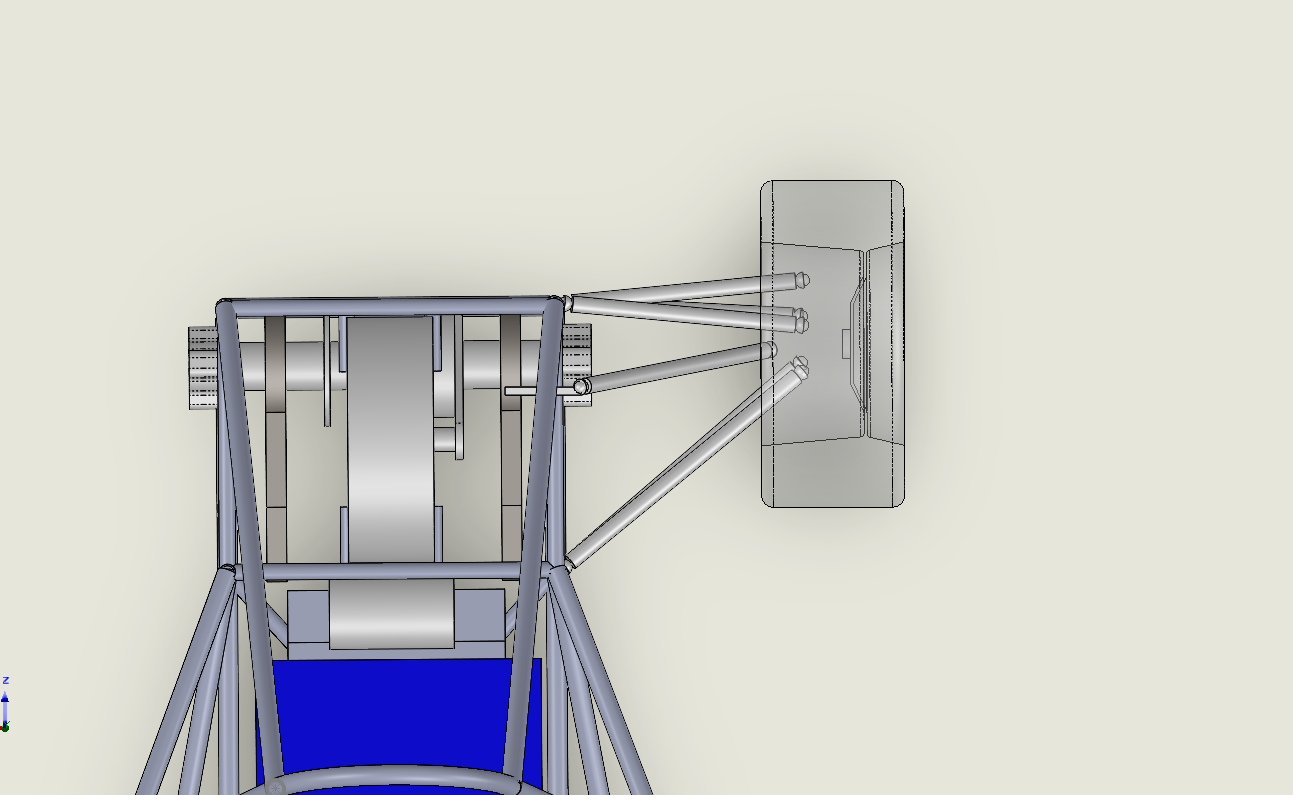
\includegraphics[width=\linewidth]{figures/rear_top_view.png}
    \caption{Top view.}
\end{subfigure}\hfill
\begin{subfigure}[t]{0.49\linewidth}
    \centering
    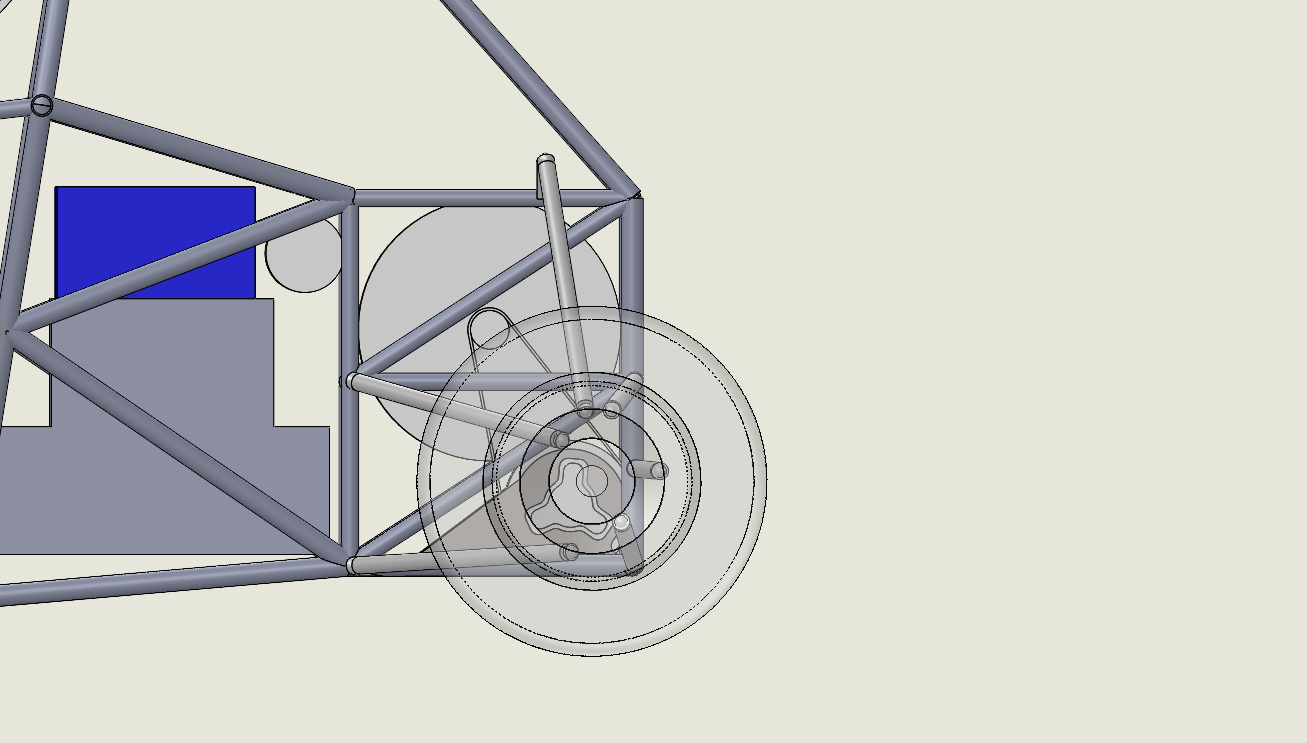
\includegraphics[width=\linewidth]{figures/rear_side_view.png}
    \caption{Side view.}
\end{subfigure}
\caption{CAD views of the rear multi-link wheel assembly. The top view identifies the rear-mounted toe link and the forward pushrod; the side view shows the shallow locating links and steep pushrod.}
\label{fig:rear_views_wheel}
\end{figure}

The suspension is described as a rear multi-link layout with five wheel-locating links plus a pushrod. The wheel-locating links are the fore/aft upper links, fore/aft lower links and rear-mounted toe link. The pushrod transfers wheel motion to the spring-damper actuation path and is not counted as a primary wheel-locating link. The chassis-side hardpoints are intentionally simple and approximately rectangular. The kinematic design work is concentrated at the upright side, where ball-joint pickup positions define anti-squat, toe-link angle and bump-steer response.

This packaging choice also improves design clarity. A welded chassis-side pickup is expensive to move once the frame is built, whereas an upright-side bracket can include machined spacers, alternative shim packs and measured setup positions. The design therefore separates structural simplicity from kinematic adjustability. The rear frame provides the load path and protects the drivetrain bay; the upright bracket design provides the final setup freedom. This is particularly valuable because the chosen toe and anti-squat values are intended as starting points for testing, not as unchangeable answers.

\subsection{Upright-side hardpoints and setup adjustability}
The 100\% anti-squat and \SI{0.15}{\degree} static rear toe-in values are educated starting values rather than fixed final settings. Formula Student setup work must account for measurement uncertainty, hardpoint tolerance, tyre behaviour and test feedback; quick adjustment of toe, camber and ride-height related variables is therefore good practice \parencite{zxOptimumGtips}.

The upright-side joint centres are implemented using brackets with shim or spacer packs. Vertical shims at the upright-side control-link pickups change the side-view link angles and therefore the anti-squat percentage. Vertical adjustment at the toe-link pickup changes the toe-link angle through wheel travel and tunes bump steer. Lateral shims set static camber and toe. Fore-aft shimming is not used because it is less repeatable under suspension load. Link lengths are set initially and then fixed, so trackside setup is mainly performed with shim packs.

\begin{table}[H]
\centering
\caption{Planned upright-side adjustment strategy.}
\label{tab:shim_strategy_wheel}
\setlength{\tabcolsep}{4pt}
\begin{tabularx}{\linewidth}{|>{\raggedright\arraybackslash}p{0.30\linewidth}|>{\raggedright\arraybackslash}X|>{\raggedright\arraybackslash}X|}
\hline
\textbf{Adjustment feature} & \textbf{Primary effect} & \textbf{Use in testing} \\
\hline
Vertical control-link shims & Side-view link angle and instant-centre position & Anti-squat tuning around the 100\% starting target \\
\hline
Vertical toe-link pickup adjustment & Toe-link angle relative to wheel travel & Bump-steer / toe-curve tuning \\
\hline
Lateral shim packs & Lateral joint-centre position & Static camber and toe correction \\
\hline
Toe-link length & Nominal toe during build & Initial setup, then fixed \\
\hline
\end{tabularx}
\end{table}

\begin{figure}[H]
\centering

\includegraphics[width=0.78\linewidth]{figures/rear_susp_motion.png}
\caption{Rear suspension motion view used to check that the toe link, pushrod and wheel-locating links remain separated and inspectable through the expected travel range.}
\label{fig:rear_motion_wheel}
\end{figure}

\subsection{Preliminary link angles and force basis}
Screenshot-derived side-view measurements show shallow locating-link angles of approximately X to \SI{12}{\degree} relative to horizontal and a much steeper pushrod angle of approximately X to \SI{80}{\degree}. The final CAD hardpoint table records the exact upper, lower and toe-link angles as X\(^{\circ}\), X\(^{\circ}\) and X\(^{\circ}\). The force-analysis design basis is \SI{230}{kg} vehicle mass and \SI{1.3}{g} maximum acceleration:
\begin{equation}
F_{x,\mathrm{total}} = ma = 230 \times 1.3 \times 9.81 \approx \SI{2.93}{kN}.
\end{equation}
If the two driven rear wheels share the load equally, \(F_{x,\mathrm{wheel}} \approx \SI{1.47}{kN}\). With the nominal anti-squat line angle of \SI{12.7}{\degree}, the idealised vertical jacking component is
\begin{equation}
F_{z,\mathrm{AS}} \approx F_{x,\mathrm{wheel}}\tan(12.7^\circ)
\approx \SI{0.33}{kN}
\end{equation}
per rear wheel.

For a representative side-view link angle of \(\alpha=\SI{10}{\degree}\), the axial force associated with the anti-squat component is
\begin{equation}
N_{\mathrm{AS,link}}\approx\frac{F_{z,\mathrm{AS}}}{2\sin\alpha}
=\frac{0.33}{2\sin10^\circ}\approx\SI{0.95}{kN}.
\end{equation}
The longitudinal contribution is
\begin{equation}
N_{x,\mathrm{link}}\approx\frac{F_{x,\mathrm{wheel}}}{2\cos\alpha}
=\frac{1.47}{2\cos10^\circ}\approx\SI{0.75}{kN}.
\end{equation}
The indicative link force is therefore about \(\sqrt{0.95^2+0.75^2}\approx\SI{1.2}{kN}\) before safety factors and transient loads. The wheel-locating links are selected as 4130 chromoly steel tube, nominally \SI{12.7}{mm} outside diameter and \SI{1.2}{mm} wall thickness, with threaded inserts and rod ends. Uprights are machined from 7075-T6 aluminium, with steel or aluminium shim packs and 4130 steel chassis brackets where welded load paths are needed.

\subsection{Anti-squat and dynamic toe-control strategy}
Anti-squat geometry limits rear suspension compression during acceleration \parencite{zxSuspensionSecretsAntiSquat}. The initial target is 100\% anti-squat, corresponding to a \SI{12.7}{\degree} side-view force line. This value is a rational reference point for an acceleration-only car because the design objective is launch stability and rear geometry control, not all-round handling. It is not treated as a proven optimum; if testing shows excessive jacking or wheel hop, vertical shims at the upright-side pickups reduce the effective anti-squat.

The static rear toe target is \SI{0.15}{\degree} toe-in. This gives initial straight-line stability, while the dynamic target is approximately zero rear toe at speed to reduce scrub. The contact-patch force at speed is
\begin{equation}
F_{x,\mathrm{rear}}\approx ma+D+F_{rr},
\end{equation}
so the anti-squat geometry responds not only to the force accelerating the vehicle, but also to the force required to overcome drag and rolling resistance. Drag also acts above ground level. Assuming the effective centre of pressure is higher than the centre of mass, the rear load-transfer contribution can be estimated as
\begin{equation}
\Delta N_{\mathrm{rear}}\approx\frac{ma h_{\mathrm{CG}}+D z_D}{L}.
\end{equation}
With the final aerodynamic model, \(D=X\,\mathrm{N}\) at X km/h and \(z_D=X\,\mathrm{m}\). This gives X N additional rear load transfer and a rear jacking displacement of X mm. Reading from the toe curve, the rear toe at X km/h is X\(^{\circ}\), satisfying the target of approximately zero toe at speed.

\figbox{30mm}{Rear toe curve placeholder: rear toe angle against wheel displacement or vehicle speed, showing \SI{0.15}{\degree} static toe-in and approximately zero toe at X km/h.}

\subsection{Single inboard brake acting on the LSD}
The rear brake acts on the LSD. This is the clearest rule-facing description because the Formula Student UK rules explicitly allow a single brake acting on a limited-slip differential \parencite{zxFSUK2026Rules}. The layout removes rear wheel-end brake discs and calipers, reducing rear unsprung mass and simplifying the upright package. The estimated saving is \SI{3.6}{kg} of rear unsprung mass and \SI{0.9}{kg} total mass relative to a conventional outboard rear brake arrangement.

\begin{table}[H]
\centering
\caption{Rear brake bill-of-materials comparison.}
\label{tab:bom_mass_wheel}
\setlength{\tabcolsep}{4pt}
\begin{tabularx}{\linewidth}{|>{\raggedright\arraybackslash}X|>{\raggedright\arraybackslash}p{0.22\linewidth}|>{\raggedright\arraybackslash}p{0.20\linewidth}|>{\raggedright\arraybackslash}X|}
\hline
\textbf{Layout} & \textbf{Rear unsprung mass effect} & \textbf{Total mass effect} & \textbf{Implication} \\
\hline
Two outboard rear brakes & Baseline & Baseline & Conventional but heavier wheel-end package \\
\hline
Single inboard brake acting on LSD & \(-\SI{3.6}{kg}\) & \(-\SI{0.9}{kg}\) & Lower rear corner mass and freer upright packaging \\
\hline
\end{tabularx}
\end{table}

The final brake package uses a Wilwood GP200 caliper, an X mm steel disc and an aluminium caliper mount tied into the rear frame bay. Brake design remains safety-critical: hydraulic pressure, piston area, effective radius, pedal force, brake balance and thermal capacity must be checked according to normal brake-design practice \parencite{zxLimpert2011}. The Formula Student rules also require protection from drivetrain failure and moving parts \parencite{zxFSUK2026Rules}.

\begin{figure}[H]
\centering
\begin{subfigure}[t]{0.49\linewidth}
    \centering
    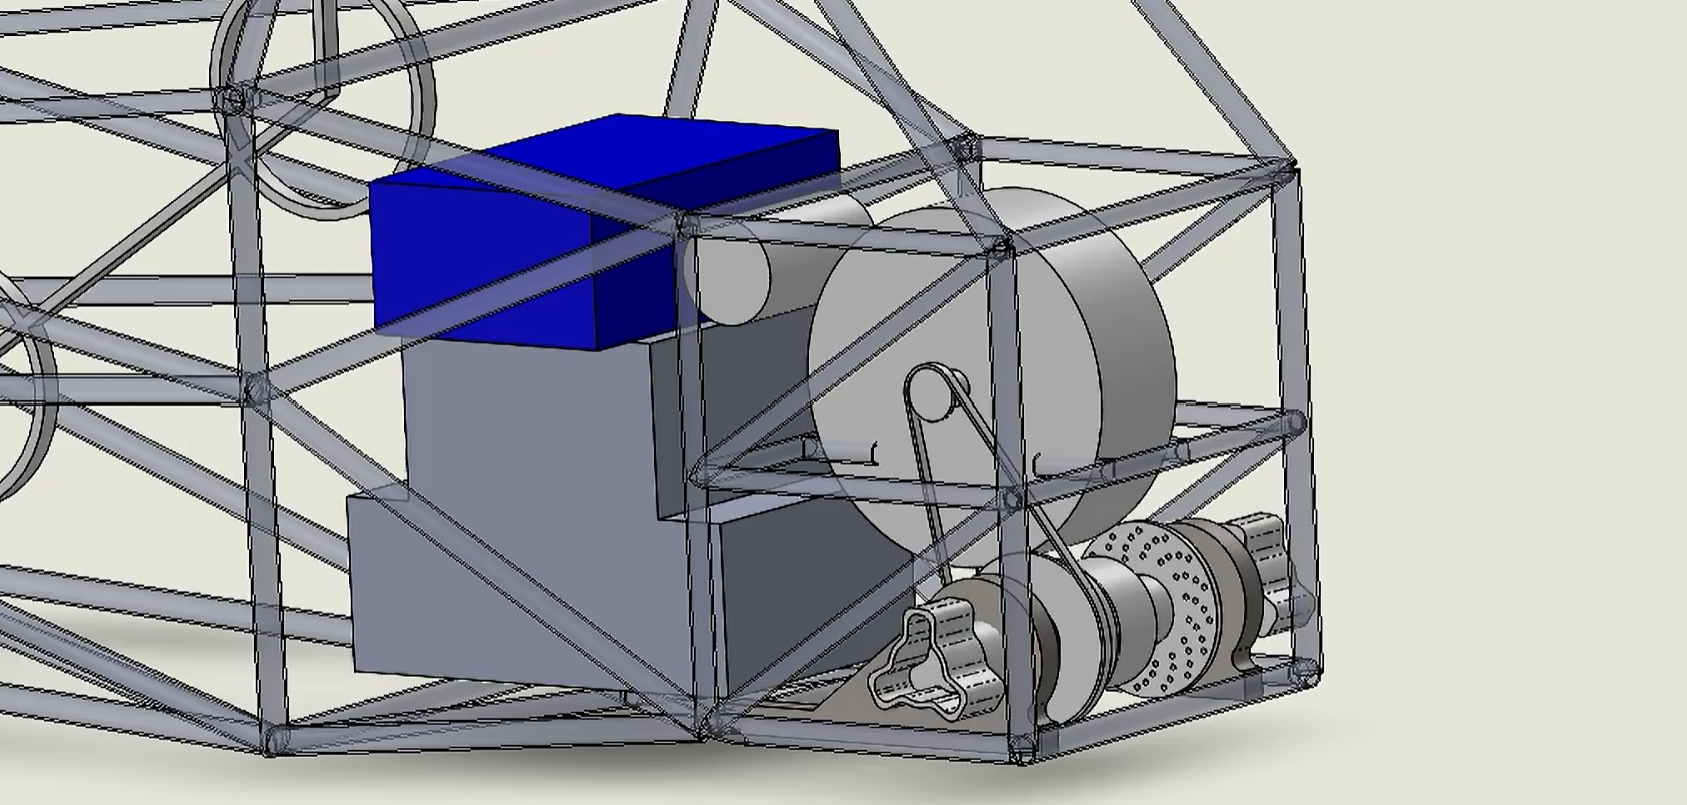
\includegraphics[width=\linewidth]{figures/powertrain_view.png}
    \caption{Central drivetrain bay for the LSD brake concept.}
\end{subfigure}\hfill
\begin{subfigure}[t]{0.49\linewidth}
    \centering
    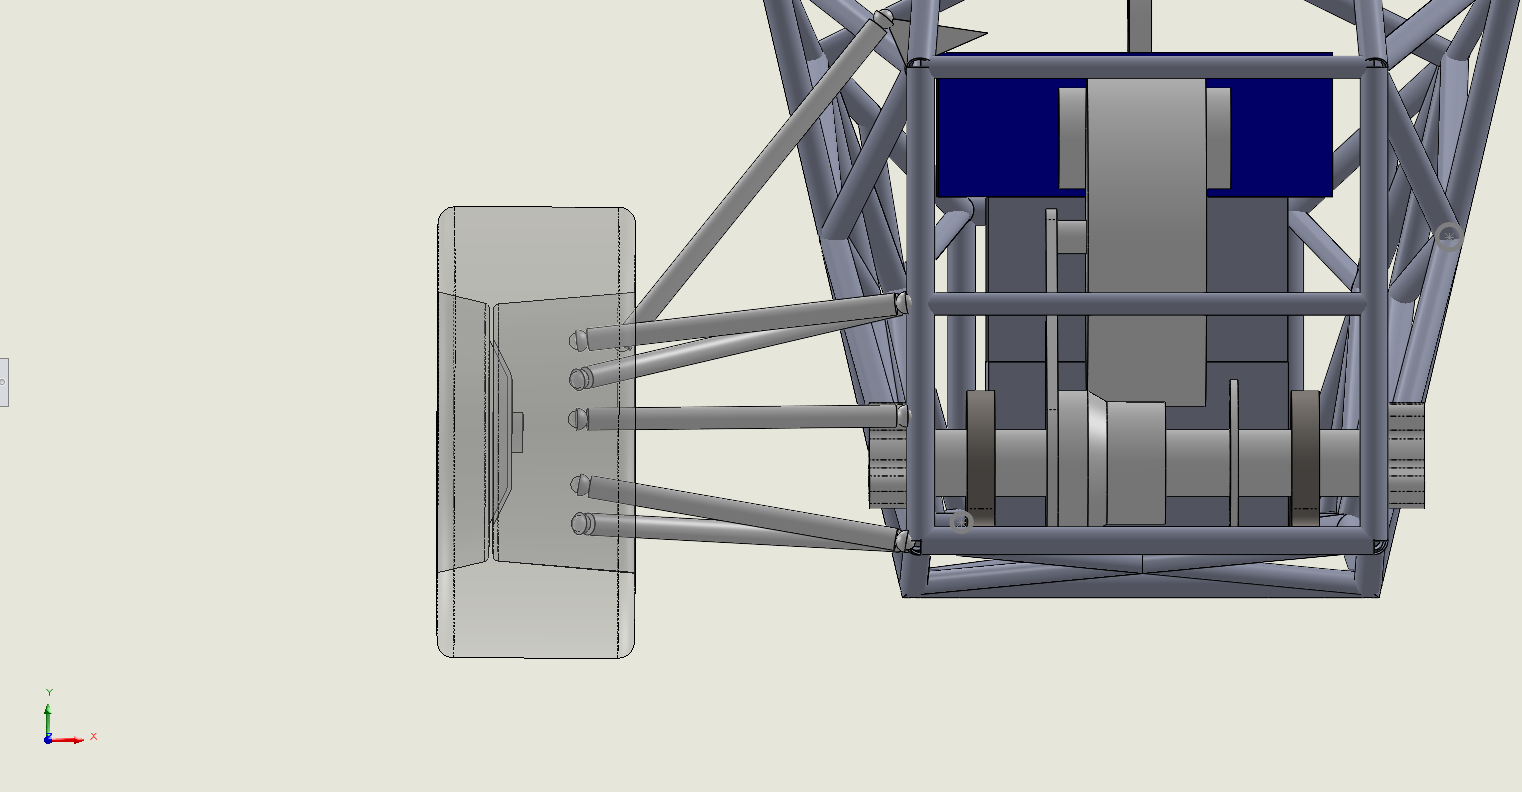
\includegraphics[width=\linewidth]{figures/rear_inboard_view.png}
    \caption{In-car rear view of the LSD/final-drive region.}
\end{subfigure}
\caption{Rear powertrain and brake integration region.}
\label{fig:rear_powertrain_package_wheel}
\end{figure}

\subsection{Rear assembly risks and mitigations}
The rear design integrates wheel location, spring-damper actuation, toe control, anti-squat tuning, drivetrain output and braking. The main risks are hardpoint sensitivity, excessive anti-squat, incorrect toe-at-speed behaviour and brake/drivetrain integration. These are mitigated through shim-adjustable upright-side pickups, load-based link sizing, a tunable toe-link pickup and a protected inboard brake package. The rear assembly is therefore not a fixed one-shot geometry; it is a tunable acceleration-focused axle concept.

\begin{table}[H]
\centering
\caption{Rear assembly risks and design mitigations.}
\label{tab:rear_risks_wheel}
\setlength{\tabcolsep}{4pt}
\begin{tabularx}{\linewidth}{|>{\raggedright\arraybackslash}p{0.25\linewidth}|>{\raggedright\arraybackslash}X|>{\raggedright\arraybackslash}X|}
\hline
\textbf{Risk} & \textbf{Effect on vehicle} & \textbf{Mitigation in design} \\
\hline
Hardpoint sensitivity & Toe curve or anti-squat differs from design intent & Upright-side shim packs and CAD coordinate checks \\
\hline
Excessive jacking & Wheel hop or harsh launch response & 100\% anti-squat treated as adjustable starting target \\
\hline
Incorrect toe-at-speed response & Too much scrub or unstable toe-out & Rear toe link, vertical pickup adjustment and lateral shim setting \\
\hline
Brake/drivetrain interaction & Concentrated central brake torque and protection requirement & Brake acts on LSD; guard, torque and failure-mode checks included \\
\hline
\end{tabularx}
\end{table}

\section{Front wheel assembly, steering and braking design}

The front wheel assembly is deliberately conventional. The front suspension is a compact double-wishbone arrangement using 4130 steel links, 7075-T6 aluminium uprights and rod-end joints with misalignment spacers. Its role is to locate the front wheels, maintain straight-line tracking and support steering and braking. Static camber is X\(^{\circ}\), front toe is X\(^{\circ}\), and the bump-steer target is less than X\(^{\circ}\) over the expected front wheel travel.

The steering system uses a compact rack-and-pinion layout with a continuous-perimeter steering wheel, quick-release hub, steering column, compact rack, tie rods and steering arms. A direct column is used where packaging allows; one high-quality universal joint is used if the final column angle requires it. The rack is mechanically attached to the primary structure, and steering stops act on the rack. This low-risk choice reflects the Formula Student steering requirements and keeps the main novelty in the rear assembly \parencite{zxFSUK2026Rules,zxFSG2026Rules}.

The front brakes provide the main inspection confidence and braking capacity. They use small outboard discs, Wilwood GP200 calipers and a conventional hydraulic circuit. The rear LSD brake reduces rear wheel-end mass, but the overall brake system still uses two independent hydraulic circuits as required by the rules \parencite{zxFSUK2026Rules}. The final brake-balance calculation gives X\% front bias and X\% rear bias at a pedal force of X N.

\begin{table}[H]
\centering
\caption{Front steering and braking elements retained for low-risk compliance.}
\label{tab:front_elements_wheel}
\setlength{\tabcolsep}{4pt}
\begin{tabularx}{\linewidth}{|>{\raggedright\arraybackslash}p{0.27\linewidth}|>{\raggedright\arraybackslash}p{0.28\linewidth}|>{\raggedright\arraybackslash}X|}
\hline
\textbf{Element} & \textbf{Design choice} & \textbf{Reason} \\
\hline
Steering gear & Compact rack-and-pinion & Direct mechanical steering with rack-mounted stops \\
\hline
Column route & Direct column or one U-joint & Low free play and visible mechanical joints \\
\hline
Front brakes & Outboard discs and GP200 calipers & Conservative inspection and braking capacity \\
\hline
Front links & 4130 steel double-wishbone links & Simple load paths and reliable fabrication \\
\hline
\end{tabularx}
\end{table}

%\figbox{30mm}{Front suspension, steering and brake drawing placeholder: double-wishbone links, upright, steering arm, rack/tie rods and front brake package.}
\begin{figure}[H]
\centering
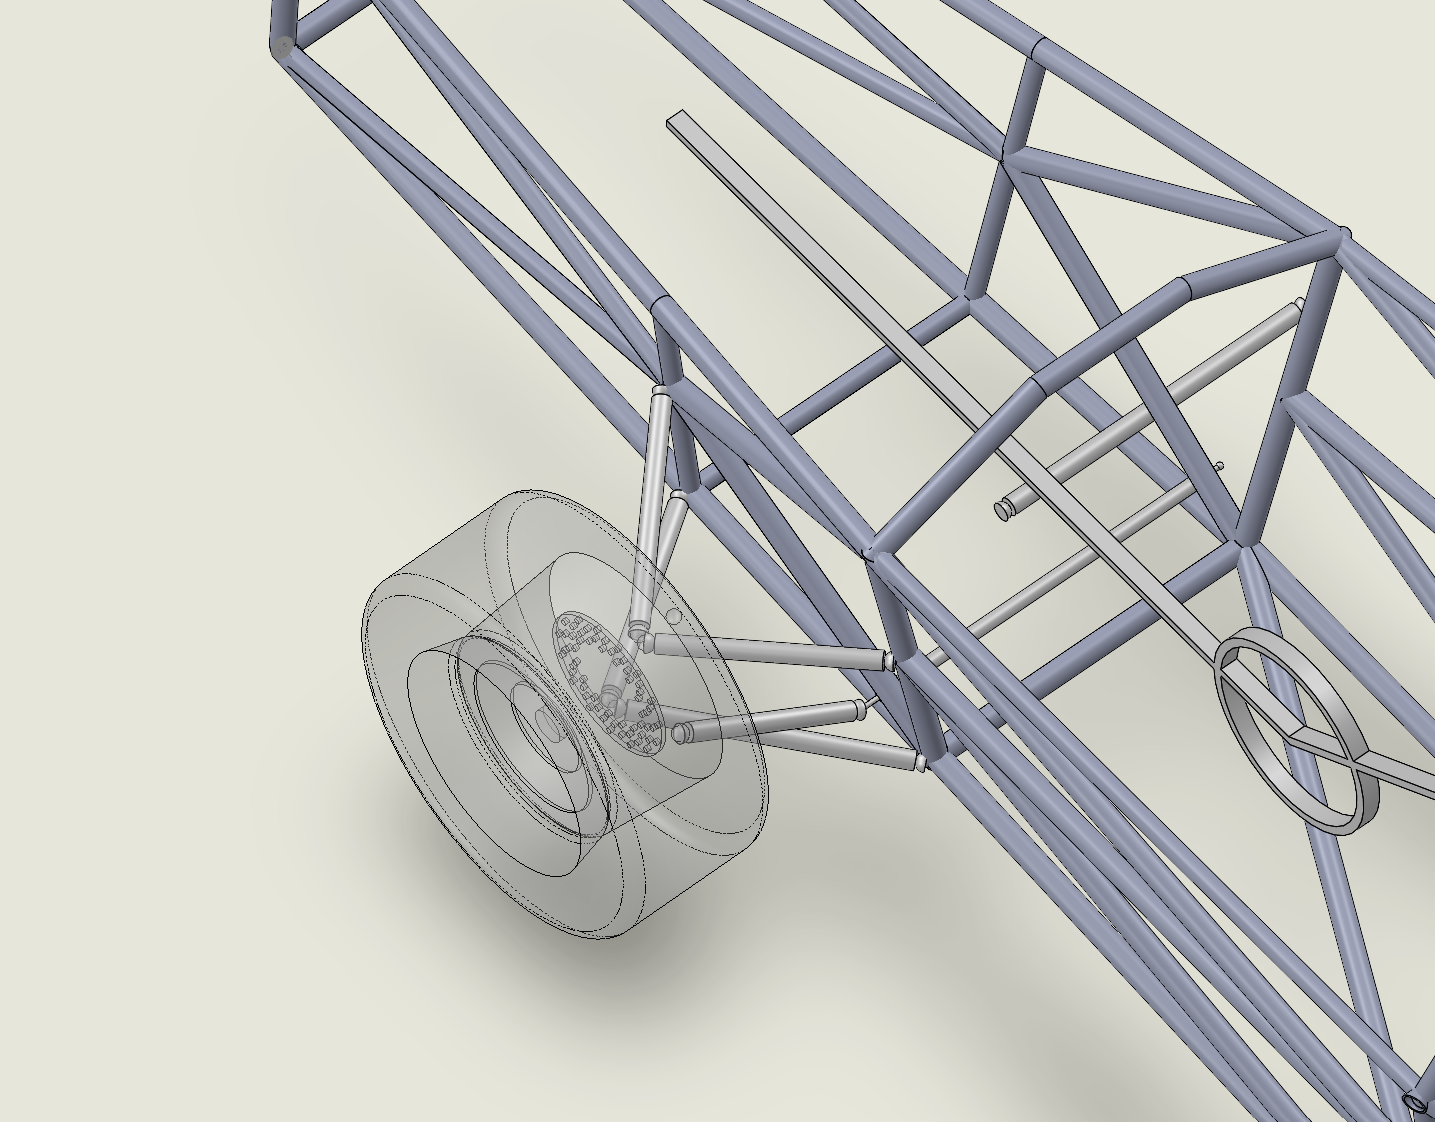
\includegraphics[width=0.78\linewidth]{figures/Front_Preview.png}
\caption{Preview of the front suspension and strring rack layout.}
\label{fig:front_preview}
\end{figure}

\section{System integration and teamwork}

The rear suspension was developed with the chassis, drivetrain, braking and vehicle-dynamics work rather than as an isolated mechanism. The simple rectangular chassis-side hardpoint arrangement gives manufacturable load paths and reduces the risk that late setup changes require chassis redesign. The upright-side shim system then provides the tuning freedom.

The powertrain and rear suspension occupy the same rear bay. The LSD, final drive, chain, brake disc, caliper, links and pushrod must all maintain clearance. The brake acts on the LSD, so its mount and guarding are part of the drivetrain package as well as the braking package. The vehicle-dynamics interface provides the \SI{230}{kg}, \SI{1.3}{g} load case, centre-of-mass height X m, centre-of-pressure height X m and drag at X km/h.

\begin{table}[H]
\centering
\caption{Subsystem interfaces used to keep the wheel assembly consistent with the vehicle.}
\label{tab:interfaces_wheel}
\setlength{\tabcolsep}{4pt}
\begin{tabularx}{\linewidth}{|>{\raggedright\arraybackslash}p{0.22\linewidth}|>{\raggedright\arraybackslash}X|>{\raggedright\arraybackslash}X|}
\hline
\textbf{Interface} & \textbf{Information exchanged} & \textbf{Design response} \\
\hline
Chassis & Hardpoint envelope and bracket load paths & Rectangular chassis-side pickups retained \\
\hline
Drivetrain & LSD, final drive and chain line & Brake and rear links packaged around central drivetrain bay \\
\hline
Vehicle dynamics & Mass, acceleration, drag and toe targets & Anti-squat and toe strategy tuned for acceleration run \\
\hline
Braking & Caliper/disc package and hydraulic layout & Single LSD brake integrated with front hydraulic circuit \\
\hline
Steering & Rack and tie-rod geometry & Conventional front steering retained for low risk \\
\hline
\end{tabularx}
\end{table}

Shared CAD reviews, mass-budget updates and rule checks were used to control these interfaces. This is important because the rear axle is not only a suspension design; it is a combined suspension, brake and drivetrain module. The design therefore satisfies the engineering requirement that individual work remains connected to the wider group design rather than optimising one isolated component.
\iffalse
\section{Evidence, limitations and final verification}

The design evidence consists of Pugh matrices, CAD packaging, component selection, preliminary anti-squat geometry, link-force calculations, the rear brake mass comparison and subsystem interface checks. The final verification values are: anti-squat line angle X\(^{\circ}\), anti-squat percentage X\%, static rear toe X\(^{\circ}\), toe at X km/h equal to X\(^{\circ}\), rear jacking displacement X mm, front bump-steer range X\(^{\circ}\), front brake torque X Nm, rear LSD brake torque X Nm and maximum suspension-link axial force X kN with a factor of safety of X.

\begin{table}[H]
\centering
\caption{Final design evidence to be reported from CAD and calculation outputs.}
\label{tab:evidence_wheel}
\setlength{\tabcolsep}{4pt}
\begin{tabularx}{\linewidth}{|>{\raggedright\arraybackslash}p{0.30\linewidth}|>{\raggedright\arraybackslash}X|>{\raggedright\arraybackslash}X|}
\hline
\textbf{Evidence item} & \textbf{Reported value} & \textbf{Design purpose} \\
\hline
Anti-squat construction & 12.7\(^{\circ}\), X\% after final CAD check & Confirms launch geometry target \\
\hline
Toe curve & 0.15\(^{\circ}\) static, X\(^{\circ}\) at X km/h & Confirms low-scrub speed condition \\
\hline
Suspension link load & X kN maximum, factor of safety X & Sizes 4130 links and brackets \\
\hline
Brake torque & X Nm front, X Nm rear LSD & Confirms braking compliance and balance \\
\hline
Mass comparison & -3.6 kg unsprung, -0.9 kg total & Justifies inboard LSD brake \\
\hline
\end{tabularx}
\end{table}

The main limitation is specialisation. A 100\% anti-squat starting target increases sensitivity to hardpoint tolerance, bracket stiffness and compliance. This is acceptable for an acceleration-only vehicle but is not claimed as an all-round Formula Student optimum. The dynamic toe strategy depends on drag, centre-of-pressure height and measured toe curve; the assumption \(z_D>h_{\mathrm{CG}}\) must be checked against the aerodynamic model. The LSD brake layout saves mass but concentrates braking torque in the central drivetrain package, requiring guarding, torque capacity and inspection access.
\fi
\section{Conclusion}

This chapter has presented the wheel assembly, suspension, steering and braking design for the acceleration-only Formula Student UK vehicle. The front systems are intentionally conventional: they provide controllability, braking confidence and rule compliance. The main contribution is the rear wheel assembly, where multi-link kinematics, dynamic toe behaviour and inboard braking are integrated.

The rear suspension uses five wheel-locating links plus a pushrod. The chassis-side pickups are simple and rectangular, while the upright-side hardpoints and shim packs provide tuning. The 100\% anti-squat target, corresponding to a \SI{12.7}{\degree} side-view force line, is an educated starting point for launch control. The \SI{0.15}{\degree} static rear toe-in is likewise an initial setup value, intended to move towards approximately zero toe at speed as the anti-squat and drag-related load state changes.

The rear brake acts on the LSD and removes outboard rear brake hardware. The expected saving is \SI{3.6}{kg} unsprung mass and \SI{0.9}{kg} total mass. The result is not a generic suspension package, but an acceleration-event-specific rear axle concept: start from a rational rear-traction setup, make the geometry adjustable, and reduce wheel-end mass while retaining rule-compliant steering and braking systems.

\compactbib
\end{refsection}

\begin{refsection}
\graphicspath{{../Yuze Jiang/Engineering/figures/}{../Yuze Jiang/Engineering/}}
% --- BEGIN INLINE: Yuze Jiang/Engineering/main.tex ---
\chapterauthor{Powertrain Design}{Yuze Jiang}

\section{Powertrain Overview}

\subsection{Design Objective}

This project focuses on the design of a powertrain system for a Formula Student race car, targeting the \SI{75}{\meter} straight-line acceleration event only.

The objective of this event is to minimise the time required to travel a short straight-line distance, under the constraints imposed by the Formula Student UK rules, as shown in Table~\ref{tab:FSUK_constraints}.

\begin{table}[H]
\centering
\small
\setlength{\tabcolsep}{24pt}

\caption{Design Constraints from FSUK Rule\cite{fs-ev-rules2026}}
\label{tab:FSUK_constraints}

\begin{tabularx}{0.4\textwidth}{l X}
\toprule
\textbf{Constraints} & \textbf{Limit} \\
\midrule
Max Power & 80\,kW \\
Max Current & 500\,A \\
\bottomrule
\end{tabularx}
\end{table}

Within these constraints, the powertrain system must efficiently convert electrical energy from a supercapacitor-based storage system into mechanical torque at the wheels, in order to maximise acceleration performance.

From basic vehicle dynamics, acceleration can be expressed as:
\begin{equation}
a = \frac{F}{m}
\end{equation}
where $F$ is the tractive force at the wheels and $m$ is the vehicle mass.

This indicates that acceleration performance can be improved by either increasing the available tractive force or reducing the overall system mass. The powertrain system directly influences the generation of tractive force through motor torque, inverter capability, and drivetrain efficiency, while system-level design choices impact the overall mass.

Therefore, the design approach focuses on maximising torque delivery while minimising system mass, resulting in a balanced optimisation of acceleration performance.
\subsection{Problem Definition}

Vehicle mass is a key factor in determining acceleration performance, as increased mass directly reduces the acceleration for a given tractive force. Minimising system weight while maintaining sufficient power supply and structural robustness is therefore a key design challenge.

The use of a supercapacitor-based energy storage system introduces additional complexity, as the supply voltage decreases during discharge. This affects the ability to sustain desired power output throughout the acceleration event and requires careful consideration in both powertrain and control system design.

In addition, the system must comply with safety requirements defined by the Formula Student rules. The shutdown circuit (SDC) provides fail-safe protection through independent hardware, operating separately from the controller to ensure safe system shutdown in fault conditions.

Other factors, such as cost and component lead time (the time between ordering and receiving the component), must also be considered. Traction-related effects, such as slip, are addressed within the control strategy, and these factors are treated as secondary considerations in this acceleration-focused design.

\subsection{Powertrain Structure}

\begin{figure}[H]
    \centering
    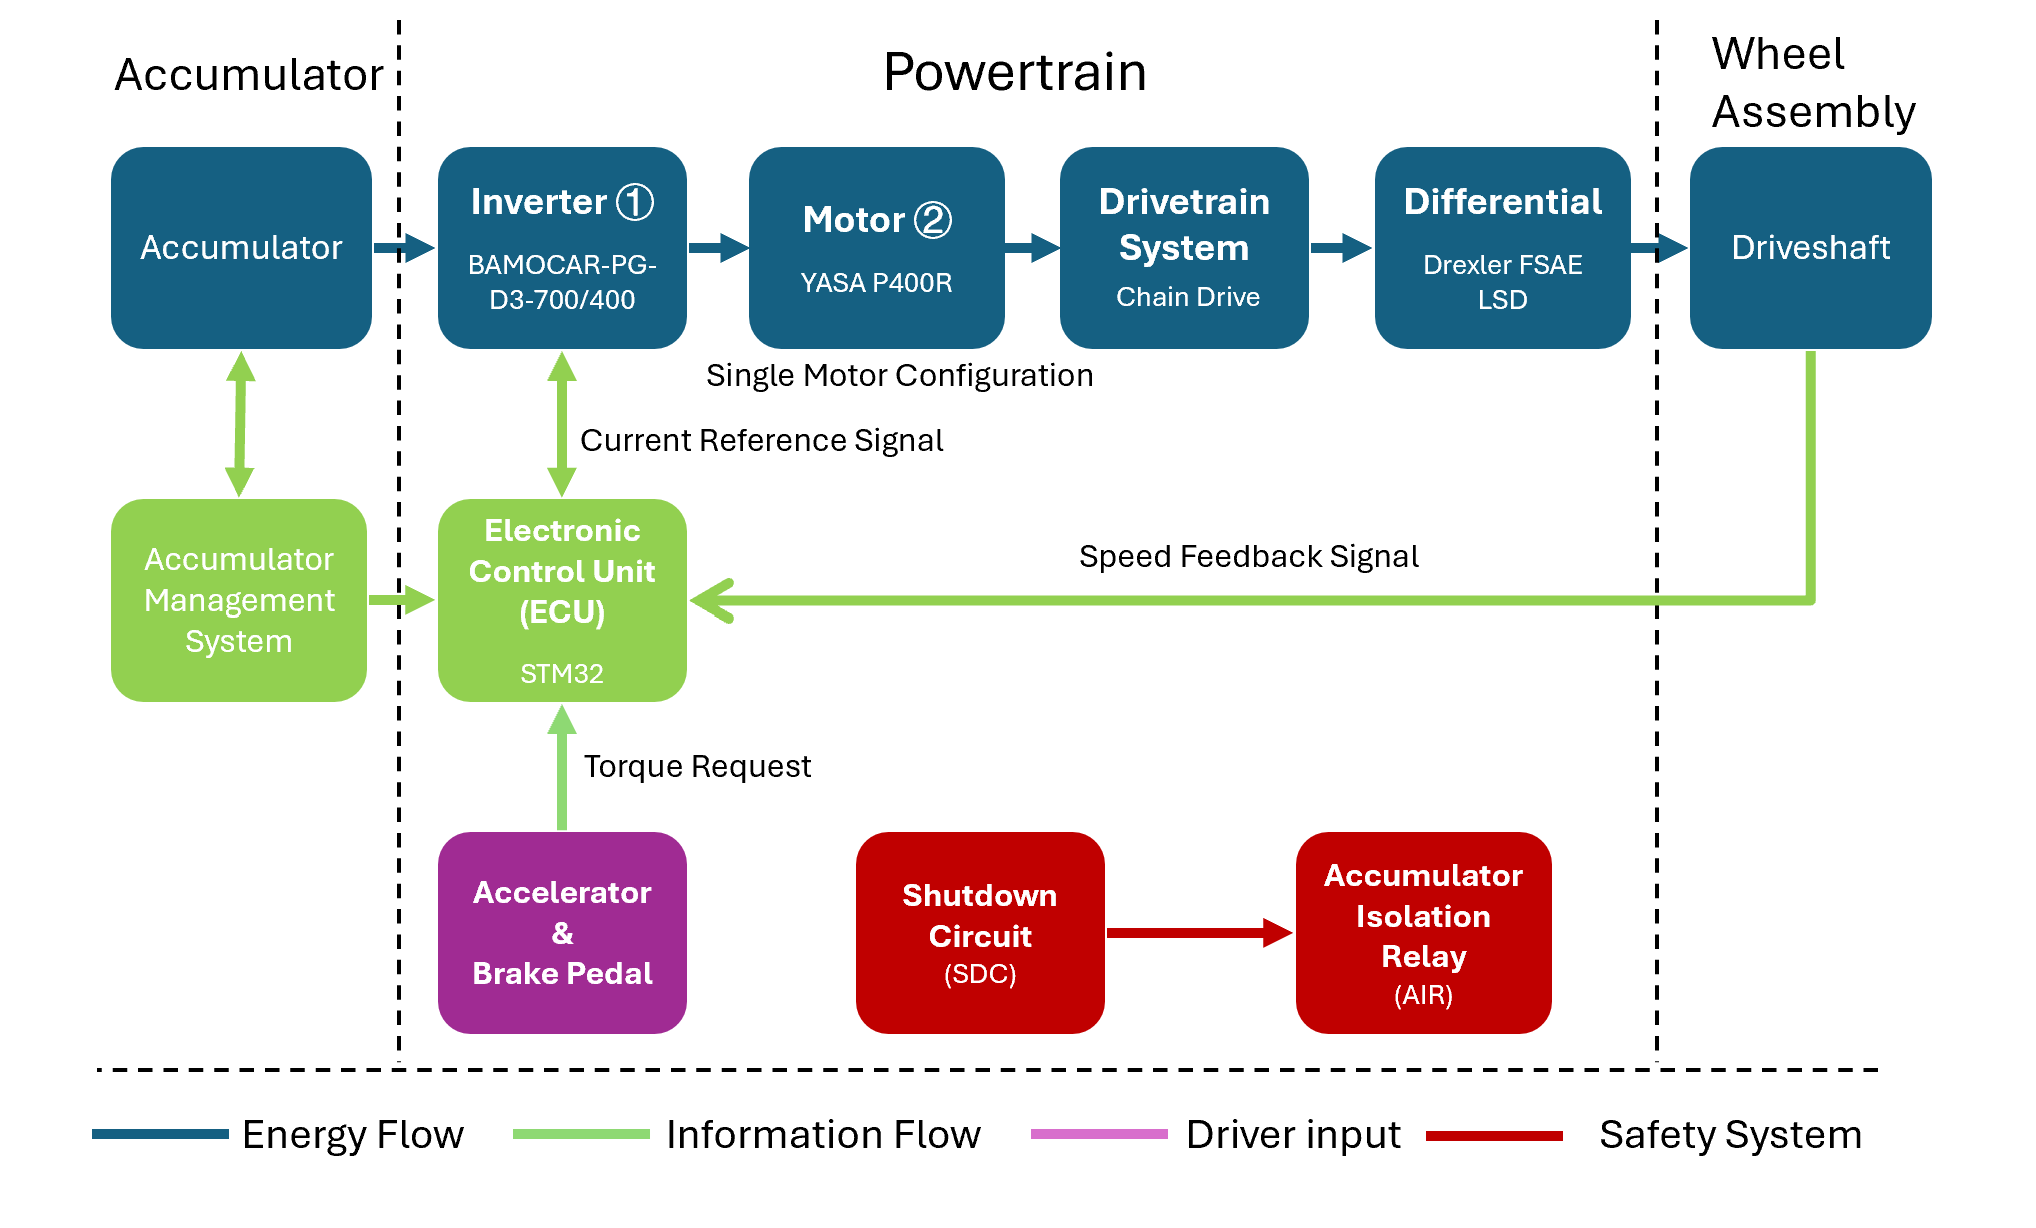
\includegraphics[width=0.8\textwidth]{powertrain_block_diagram_1.png}
    \caption{Block Diagram for Powertrain System}
    \label{fig:powertrain}
\end{figure}

The powertrain system considered in this work focuses on the components between the accumulator (battery system) and the output shaft, as illustrated in Figure~\ref{fig:powertrain}.

Electrical energy is supplied from the accumulator to the inverter, which converts DC power into controlled AC power for the motor. The motor generates torque, which is transmitted through the drivetrain and differential to the output shaft, delivering mechanical power to the wheel assembly, which is considered external to this work.

The control system operates in parallel with the powertrain hardware. Driver inputs from the accelerator and brake pedals are processed by the controller, which guarantees the system is operating under Formula Student UK Rule~\cite{fs-ev-rules2026} and then generates a torque request. This torque request is converted into a current reference signal and sent to the inverter, which regulates motor current to achieve the desired torque output.

Feedback from the powertrain hardware, in the form of shaft or wheel speed, is returned to the controller as a speed feedback signal. This enables the controller to enforce system constraints and maintain stable operation.

In addition to the control system, a shutdown circuit (SDC) provides an independent safety mechanism using non-programmable hardware. When triggered, it actuates the accumulator isolation relay (AIR) to disconnect the tractive system, ensuring fail-safe operation.

Overall, the system is designed to transfer electrical energy from the accumulator to mechanical energy at the driveshaft while maintaining controllability and safety. And a CAD drawing is shown in Figure~\ref{fig:CAD} to help visualization.

\begin{figure}
    \centering
    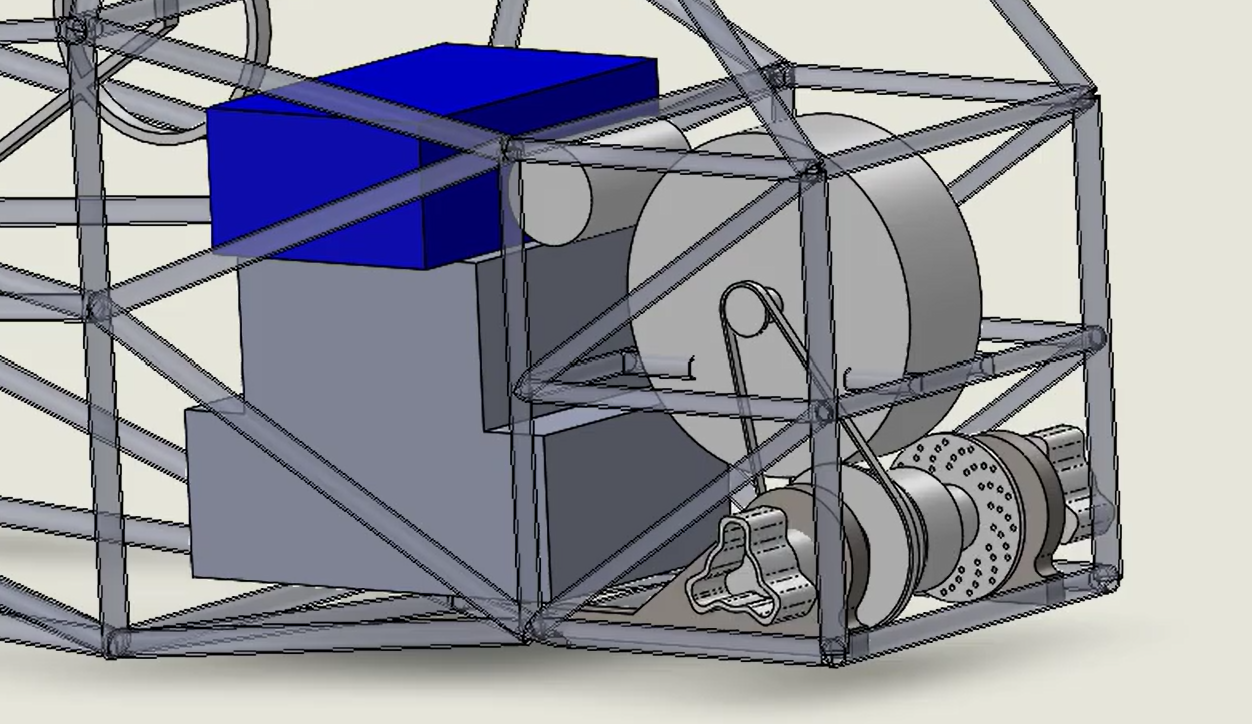
\includegraphics[width=0.75\linewidth]{CAD_Drawing.png}
    \caption{CAD Drawing for Powertrain Components (from Toby and Michael)}
    \label{fig:CAD}
\end{figure}

\section{Motor Selection}

\subsection{Motor Configuration}
% Ask Michael

The powertrain architecture adopts a centralised single-motor configuration, as determined by the overall vehicle design (based on analysis from Ziyang Xing).

A multi-motor configuration can provide advantages such as torque vectoring and improved traction control. However, for the \SI{75}{\meter} acceleration event, the vehicle primarily operates under straight-line conditions, where the benefits of torque vectoring are limited.

The selected single-motor configuration reduces drivetrain complexity and vehicle mass, which is beneficial for acceleration performance under power and current constraints. It is therefore used as the basis for subsequent motor selection and powertrain design.

\subsection{Motor Requirements}

The motor must be capable of delivering high torque, particularly at low speeds, to maximise usable traction.

It must operate within the \SI{80}{\kilo\watt} power limit and \SI{500}{\ampere} current constraint, requiring a balance between torque output and electrical demand.

Consideration is also given to system mass, cooling requirements, and integration with the inverter and drivetrain, as these factors influence overall performance and packaging.

\subsection{Candidate Motors}

Two motor families were considered for the powertrain design: the YASA P400R \cite{YASA_P400R_data_sheet} and the EMRAX 208 series\cite{EMRAX_208_data_sheet}, EMRAX 228 Series\cite{EMRAX_228_datasheet}, Cascadia iM-125DX-D\cite{Cascadia_iM125DXD_datasheet}, Cascadia iM-225\cite{Cascadia_iM225_datasheet}, YASA P400R \cite{YASA_P400R_data_sheet}, and YASA 750R\cite{YASA_750R_datasheet}. 
The EMRAX 208 and 228 series are available in both medium and high voltage variants, with different cooling configurations including air, liquid, and combined cooling.

\subsection{Selection Criteria}

The motor selection is based on a set of weighted criteria reflecting both performance requirements and practical considerations, as summarised in Table~\ref{tab:motor_selection}.

Peak torque is assigned the highest weighting, as it directly determines the tractive force that can be generated at the wheels, and hence the achievable vehicle acceleration. The relationship between motor torque, tractive force, and vehicle acceleration is given by:
\begin{equation}
F = \frac{T}{r}, \qquad
a = \frac{F}{m} = \frac{T}{mr}
\end{equation}
where $T$ is the motor torque, $r$ is the effective wheel radius, and $m$ is the vehicle mass.

However, the maximum usable tractive force is constrained not only by motor torque, but also by tyre grip at the contact patch. During launch, the vehicle operates in a traction-limited regime, where the maximum transferable force is limited by tyre adhesion. The motor must therefore provide sufficient torque to exceed this traction limit, ensuring that motor capability won't be the limiting factor in vehicle acceleration.

Vehicle dynamics simulation in Section 5.2.4 shows that the transition from the traction-limited to the power-limited regime occurs at $v^* = 15.4\ \mathrm{m\,s^{-1}}$ , at which point the required peak motor torque is $T_m^\mathrm{peak} = K_t I_\mathrm{max} = 234\ \mathrm{N\,m}$. A motor with peak torque below this threshold would become the limiting 
factor during the launch phase, directly degrading acceleration performance. Therefore, peak torque is assigned the highest weighting in the merit matrix, with $234\ \mathrm{N\,m}$ treated as the key performance threshold for this factor.

%%***
Effective power density is considered as a secondary performance indicator, influencing system mass and packaging. Since all candidate motors are capable of operating at the 80~kW competition power limit~\cite{fs-ev-rules2026}, the absolute peak power of each motor is not considered a distinguishing factor in this comparison. Therefore, the power density evaluation is normalized using the regulated maximum allowable power output, which is a pure comparison of weight.
\begin{equation}
Effective Power Density = \frac{80\ \text{kW}}{m_{\text{motor}}}
\end{equation}

Cooling System, cost, and lead time are assigned lower weightings, as they have limited impact on short-duration acceleration performance.

\subsection{Evaluation}

\begin{table}[H]
\centering
\small
\renewcommand{\arraystretch}{1}
\setlength{\tabcolsep}{4pt}

\caption{Merit Matrix for Motor Selection}
\label{tab:motor_merit_matrix}

\small
Scoring scale: 0 = poor, 1 = acceptable, 2 = good, 3 = excellent.  
Score $= \sum (\text{individual score} \times \text{weighting})$.
\label{tab:motor_selection}


\begin{tabularx}{\textwidth}{
>{\raggedright\arraybackslash}p{3.5cm}
>{\centering\arraybackslash}p{1.7cm}
>{\centering\arraybackslash}p{1.7cm}
>{\centering\arraybackslash}p{3.0cm}
>{\centering\arraybackslash}p{1.7cm}
>{\centering\arraybackslash}p{1.7cm}
>{\centering\arraybackslash}p{1.7cm}
}
\toprule

Motor 
& Cost 
& Lead Time 
& Effective Power Density 
& Peak Torque 
& Cooling System 
& \textbf{Score} \\

\midrule

\textbf{Weighting}
& 1
& 1
& 2
& 5
& 1
& {} \\

\midrule

\shortstack{EMRAX 208 Series}
& 3
& 2
& 3
& 1
& 2
& 18 \\

\shortstack{EMRAX 228 Series}
& 2
& 2
& 2
& 2
& 2
& 20 \\

\shortstack{Cascadia iM-125DX-D}
& 2
& 2
& 1
& 1
& 1
& 12 \\

\shortstack{Cascadia iM-225}
& 0
& 2
& 0
& 3
& 2
& 19 \\

\shortstack{\textbf{YASA P400R}}
& 1
& 1
& 1
& 3
& 3
& \textbf{22} \\

\shortstack{YASA 750R}
& 0
& 1
& 1
& 3
& 3
& 21 \\

\bottomrule
\end{tabularx}
\end{table}

The results show that the YASA P400R achieves the highest overall score, primarily due to its superior peak torque performance, which has the greatest influence on acceleration capability.

\subsection{Final Decision}

Based on the evaluation, the YASA P400R is selected as the motor for the powertrain system, providing the most suitable solution for the defined performance requirements.

\subsection{Motor Operation}

Following the motor selection, the operating strategy is defined to ensure compliance with the \SI{80}{\kilo\watt} power limit.

As shown in Figure~\ref{fig:motor_operation}, the YASA P400R motor is capable of delivering a peak power significantly higher than the system limit (approximately \SI{170}{\kilo\watt}). Therefore, the motor is not operated at its maximum capability. Instead, the operating point is constrained through the inverter and controller by limiting the effective operating voltage to approximately \SI{350}{\volt}.

This ensures that the motor operates within the power limit while still delivering high torque in the low-speed region, which is critical for acceleration performance. As vehicle speed increases, the operating point is dynamically adjusted through current and voltage control to maintain optimal power delivery within system constraints.


\begin{figure}
    \centering
    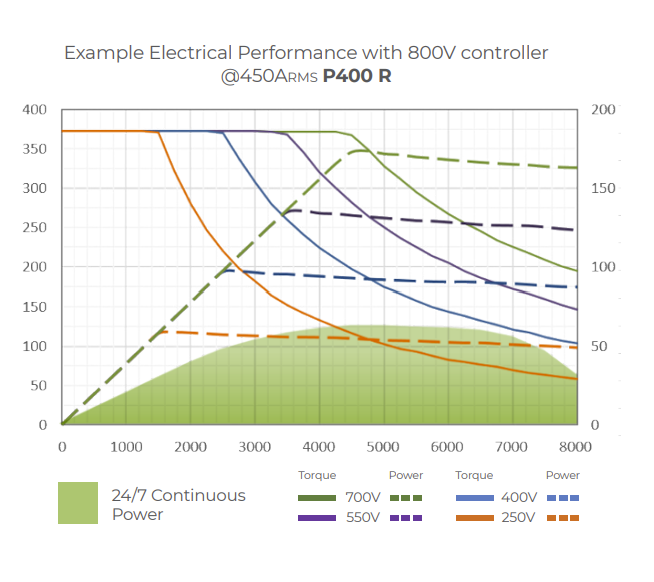
\includegraphics[width=0.7\linewidth]{YASA_Motor_Operation_Graph.png}
    \caption{YASA P400R Operation Curve\cite{YASA_P400R_data_sheet}}
    \label{fig:motor_operation}
\end{figure}

\subsection{Further Cooling System Improvements}

Although cooling requirements are not a limiting factor for the selected motor, they present an opportunity for further optimisation.

The short-duration operation of the system results in minimal heat generation:
\begin{equation}
Q = P t \eta_{\text{loss}}
= 80{,}000 \times 4 \times 0.05
= \SI{16000}{\joule}
\end{equation}

Using a motor mass of $m = \SI{28.2}{\kilogram}$ and an average specific heat capacity of $c_p \approx \SI{500}{\joule\per\kilogram\per\kelvin}$:

\begin{equation}
\Delta T
=
\frac{Q}{m c_p}
=
\frac{16000}{28.2 \times 500}
\approx
\SI{1.1}{\degreeCelsius}
\end{equation}

Even under high ambient temperatures, a temperature rise of only \SI{1.1}{\degreeCelsius} would keep the motor well below its typical continuous operating temperature of approximately \SI{50}{\degreeCelsius}, indicating negligible thermal risk during operation.

This suggests that the motor is effectively over-designed in terms of cooling for this application. Therefore, future development could explore simplified cooling configurations in collaboration with the manufacturer, potentially reducing system mass and complexity.

\section{Inverter Selection}

\subsection{Inverter Requirements}

The inverter must be compatible with the overall powertrain system, ensuring effective operation with the selected motor under the defined electrical constraints.

A key requirement is the ability to operate over a wide input voltage range, allowing flexibility in the design of the supercapacitor-based energy storage system, where the supply voltage decays during discharge.
%maybe cite something about Paul
The inverter must also support the required current and power levels while maintaining reliable integration within the powertrain system.

Several inverter options were considered for the powertrain system, including the DMC544\cite{DMC544_datasheet}
, BAMOCAR PG-D3 series\cite{BAMOCAR_data_sheet}
, CM200DX and CM200DZ\cite{CM200_data_sheet}.

These candidates provide different voltage ranges, current capabilities, and system integration characteristics, forming the basis for further evaluation. The key specifications are summarised in Table~\ref{tab:inverter_parameters}.

\subsection{Candidate Parameters}

\begin{table}[H]
\centering
\renewcommand{\arraystretch}{1}
\caption{Parameters of Candidate Inverters}
\label{tab:inverter_parameters}
\begin{tabular}{lcccccc}
\toprule
Inverter & $V_{\text{max}}$ (V) & $V_{\text{min}}$ (V) & $I_{\text{peak}}$ (A) & $P_{\text{peak}}$ (kW) & Weight (kg) & Cost (USD) \\
\midrule
DMC544 & 450 & 12 & 600 & 300 & 15.3 & 24000 \\
BAMOCAR 400/400 & 400 & 12 & 285 & 75 & 8.5 & 6300 \\
BAMOCAR 700/250 & 700 & 12 & 178 & 85 & 8.5 & 6300 \\
%need check for bamocar price
BAMOCAR 700/400 & 700 & 12 & 285 & 135 & 8.5 & 6300 \\
CM200DX & 480 & 50 & 740 & 225 & 6.75 & 8700 \\
CM200DZ & 840 & 200 & 400 & 225 & 6.75 & 9000 \\
\bottomrule
\end{tabular}
\end{table}

\subsection{Selection Criteria}

The inverter selection is conducted in two stages.

First, candidate inverters must satisfy minimum electrical constraints, including voltage, current, and power requirements, to ensure compatibility with the selected motor and system limits.

Among the feasible candidates, the selection is based on system-level performance considerations.

Voltage range is assigned the highest priority, as it determines the flexibility of the supercapacitor-based energy storage system. In this design, the minimum operating voltage is constrained at 350V to ensure stable operation within the desired motor operating region. As a result, the usable energy is primarily determined by the maximum allowable voltage. The energy stored in the supercapacitor can be expressed as:
\begin{equation}
E = \frac{1}{2} C V^2
\end{equation}
and the usable energy over the operating range is therefore:
\begin{equation}
E_{\text{usable}} = \frac{1}{2} C \left( V_{\max}^2 - V_{\min}^2 \right)
\end{equation}

With a fixed minimum voltage, a higher allowable maximum voltage increases the usable energy, allowing a reduction in the required capacitance and therefore system mass. Conversely, a limited voltage range equires more capacitor units to meet the energy demand, increasing system weight.

Additional factors such as cost, lead time, and system mass are considered with lower weighting, as they have less influence on overall performance.
\subsection{Evaluation}

Constraint-based filtering is first applied to eliminate inverters that do not meet the minimum requirements. The remaining candidates are then compared using the merit matrix shown in Table~\ref{tab:inverter_selection}.

\begin{table}[H]
\centering
\renewcommand{\arraystretch}{1}

\caption{Merit Matrix for Inverter Selection}
\label{tab:inverter_selection}

\small
Scoring scale: 0 = poor, 1 = acceptable, 2 = good, 3 = excellent.  
Weighted score $= \sum (\text{score} \times \text{weighting})$.

\begin{tabular}{lcccccc}
\toprule

Inverter 
& Constraint 
& Cost 
& Lead Time 
& Voltage Range 
& Weight 
& Score \\

\midrule

\textbf{Weighting}
& Pass/Fail
& 1
& 1
& 2
& 1
& {} \\

\midrule

DMC544 
& Pass 
& 0 
& 0 
& 0 
& 0 
& 0 \\

BAMOCAR 400/400 
& Fail 
& -- 
& -- 
& -- 
& -- 
& 0 \\

BAMOCAR 700/250 
& Fail 
& -- 
& -- 
& -- 
& -- 
& 0 \\

\textbf{BAMOCAR 700/400} 
& Pass 
& 3 
& 1 
& 2 
& 1 
& \textbf{9} \\

CM200DX 
& Pass 
& 2 
& 1 
& 1 
& 2 
& 7 \\

CM200DZ 
& Pass 
& 1 
& 1 
& 2 
& 2 
& 8 \\

\bottomrule
\end{tabular}
\end{table}

The results indicate that the BAMOCAR PG-D3-700/400 achieves the highest overall score.

This is primarily due to its wide voltage operating range, which provides greater flexibility for the supercapacitor-based energy storage system. Other candidates either have more limited voltage capability or present fewer benefits in cost, lead time, and integration.

\subsection{Final Decision}

Based on the evaluation, the BAMOCAR PG-D3-700/400 is selected as the inverter for the powertrain system, providing the most suitable solution for this application.

\section{Controller Design}

\subsection{Control Architecture}

The control system is responsible for generating motor torque demand based on driver input, while ensuring safe and stable operation through the enforcement of system constraints.  %***

As shown in Figure~\ref{fig:controller}, the controller processes sensor inputs, including accelerator and brake pedal signals, speed measurements, and accumulator measurements. These signals are used to perform plausibility checks, calculate torque demand, and enforce system constraints such as power and current limits.

\begin{figure}
    \centering
    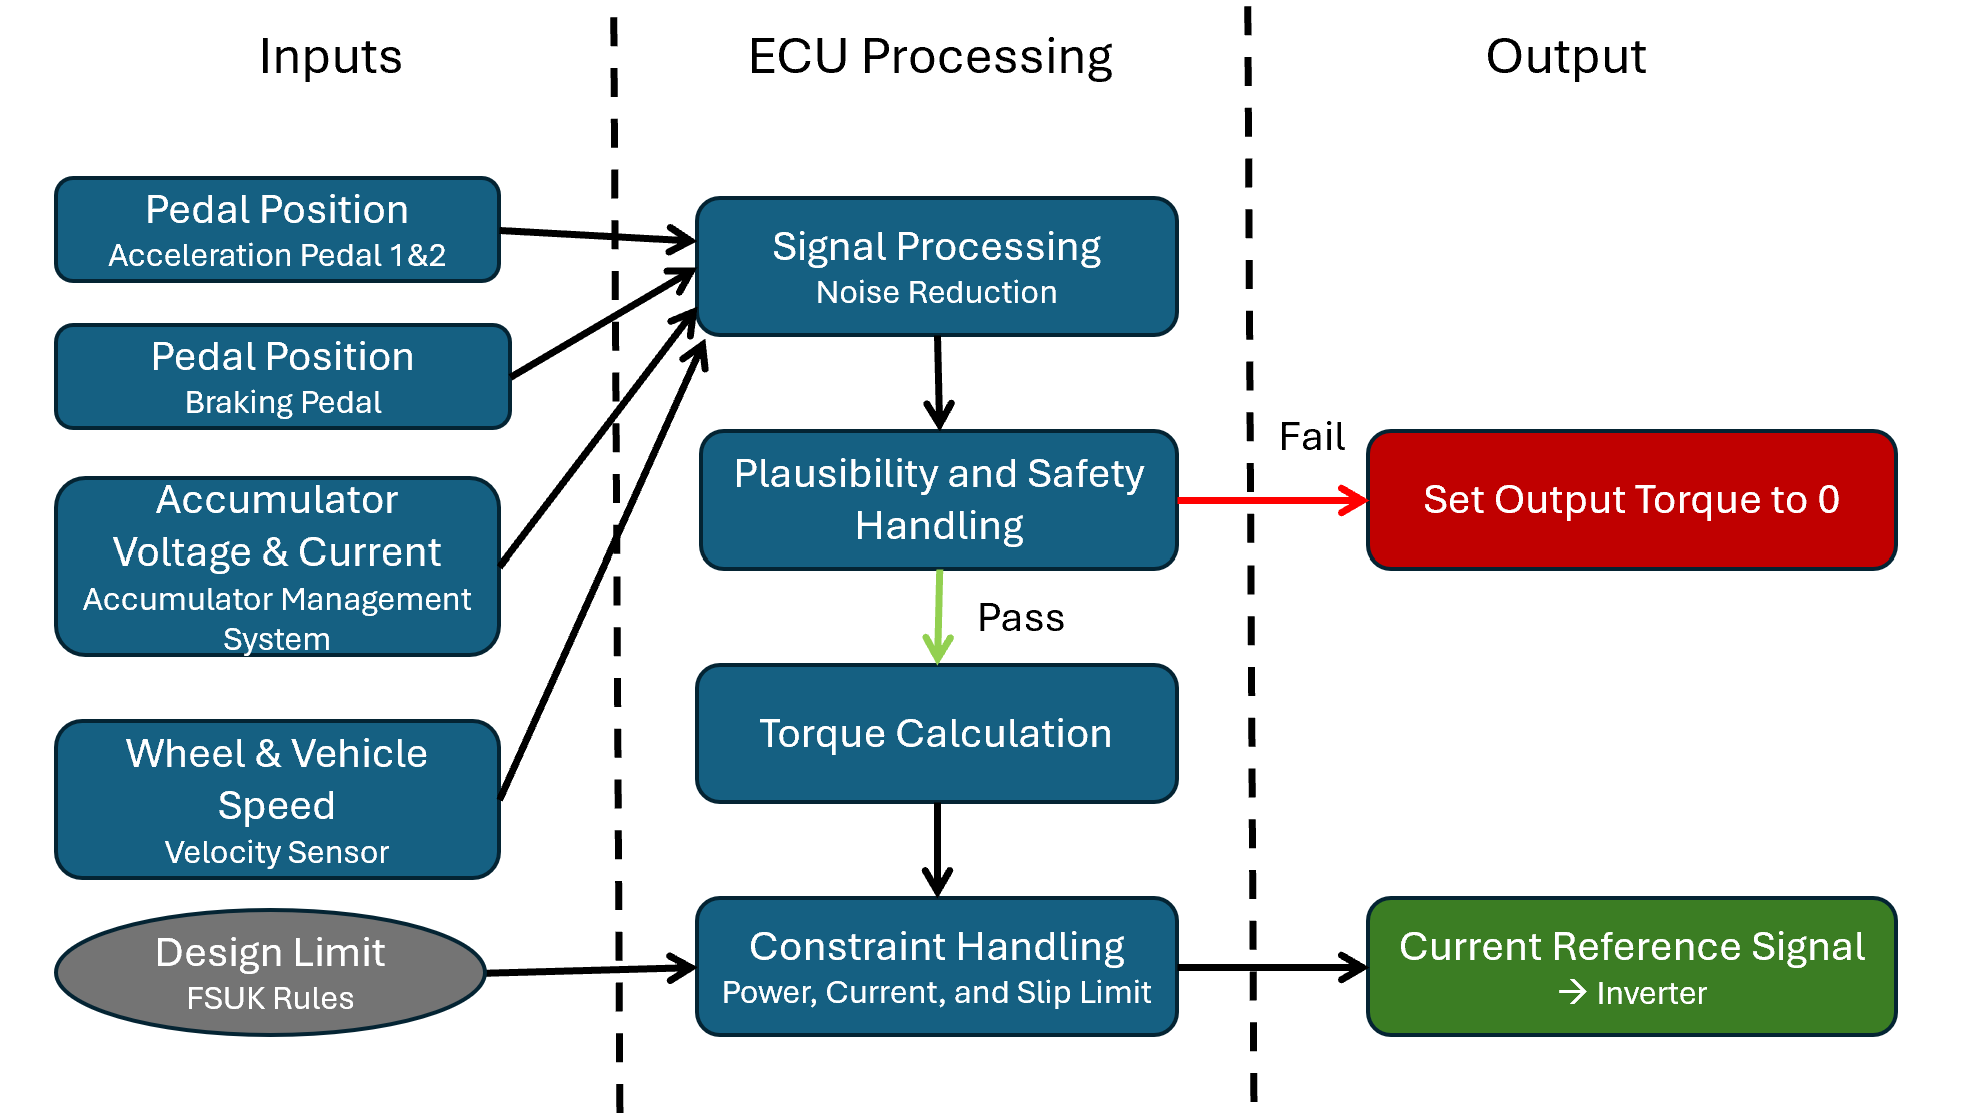
\includegraphics[width=0.9\linewidth]{Controller _Structure.png}
    \caption{Structure for Control System}
    \label{fig:controller}
\end{figure}

\subsection{Signal Processing}

The controller processes inputs from multiple sensors, including accelerator and brake pedal signals, wheel speed, and accumulator management system measurements.

Raw sensor signals are filtered to reduce noise and ensure stable inputs for control calculations. These processed signals are then used for state estimation and control logic implementation.%%\cite{filter——controller}

\subsection{Plausibility and Safety Handling}

Plausibility checks are applied to ensure the validity of critical input signals, particularly the accelerator pedal position sensors. The consistency between multiple pedal signals is monitored to detect implausible conditions in accordance with safety requirements.

If an inconsistency is detected, the torque request is immediately set to zero to ensure safe operation.

In addition, a brake override strategy is implemented, where motor torque is reduced to zero when braking is detected.

\subsection{Torque Control Strategy}
The controller calculates the required motor torque based on driver input using a feedforward approach.

Motor torque is proportional to the phase current, which can be expressed as:
\begin{equation}
T = k_t I
\end{equation}
where $k_t$ is the motor torque constant and $I$ is the motor current.

The torque demand is therefore converted into a current reference using the motor torque constant. To ensure smooth operation, torque commands are subject to rate limiting to avoid abrupt changes in output.
\subsection{Constraint and Feedback Handling}

Feedback from motor and wheel speed is used to monitor system behaviour and slip conditions. When excessive slip is detected, the torque request is reduced to maintain traction.

In addition, system constraints are enforced using battery voltage and current measurements. Power and current limits are applied to ensure operation within the defined electrical constraints.

\subsection{Controller Selection}

The controller hardware is selected to support the proposed control strategy while ensuring reliable system operation.

Several platforms were evaluated, including STM32\cite{stm32-nucleo-f4}
, Arduino Uno\cite{Arduino_uno_data_sheet}
, TI C2000\cite{TI_C200_data_sheet}
, NXP S32K\cite{NPX_S32K_data_sheet}
, and Speedgoat/dSPACE systems\cite{Speedgoat_data_sheet}.
After applying basic voltage and communication constraints, a merit matrix is used to compare the feasible options, as shown in Table~\ref{tab:controller_selection}.

\begin{table}[H]
\centering
\small
\renewcommand{\arraystretch}{1}
\setlength{\tabcolsep}{3pt}

\caption{Merit Matrix for Controller Selection}
\label{tab:controller_selection}
\small
Scoring scale: 0 = poor, 1 = acceptable, 2 = good, 3 = excellent.  
Weighted score $= \sum (\text{score} \times \text{weighting})$.
\makebox[\textwidth][c]{
\begin{tabularx}{0.95\textwidth}{p{2cm} *{7}{>{\centering\arraybackslash}X} >{\centering\arraybackslash}X}
\toprule
 ECU & Supply Voltage & Weight & Cost & Processing Time & System Latency & CAN Capability & Reliability & \textbf{Score} \\
\midrule

Weighting
& Pass/Fail & 1 & 2 & 2 & 2 & Pass/Fail & 2 & --\\
\midrule

\textbf{STM32}
& Pass & 3 & 3 & 1 & 1 & Pass & 1 & \textbf{15} \\

Arduino Uno
& Pass & 1 & 1 & 2 & 2 & Fail & 1 & -- \\

TI C2000
& Pass & 2 & 2 & 2 & 2 & Pass & 1 & 12 \\

NXP S32K
& Pass & 2 & 2 & 1 & 1 & Pass & 1 & 12 \\

\bottomrule
\end{tabularx}
}
\end{table}

The results indicate that the STM32 achieves the highest overall score due to its balanced performance in cost, weight, processing capability, communication support, and reliability.

\subsection{Final Decision}

Based on the evaluation, the STM32 platform is selected as the controller for the powertrain system.

\section{Shutdown Circuit (SDC) Design}

\subsection{Overview of Shutdown Circuit}

The shutdown circuit (SDC) is a critical safety system designed to ensure immediate disconnection of the tractive system under fault conditions. This architecture is selected to guarantee fail-safe operation through a hardware-based implementation that remains effective even in the event of controller failure.
\subsection{Shutdown Circuit Architecture}

The shutdown circuit is designed based on Formula Student UK (FSUK) safety requirements, which mandate a non-programmable, hardware-based system to ensure reliable and fail-safe operation.

The SDC is implemented as a series-connected circuit of safety devices, including monitoring systems and interlock components. All elements must remain in a closed state for normal operation, and any triggered fault will open the circuit and deactivate the tractive system.

%bigger figure
\begin{figure}
    \centering
    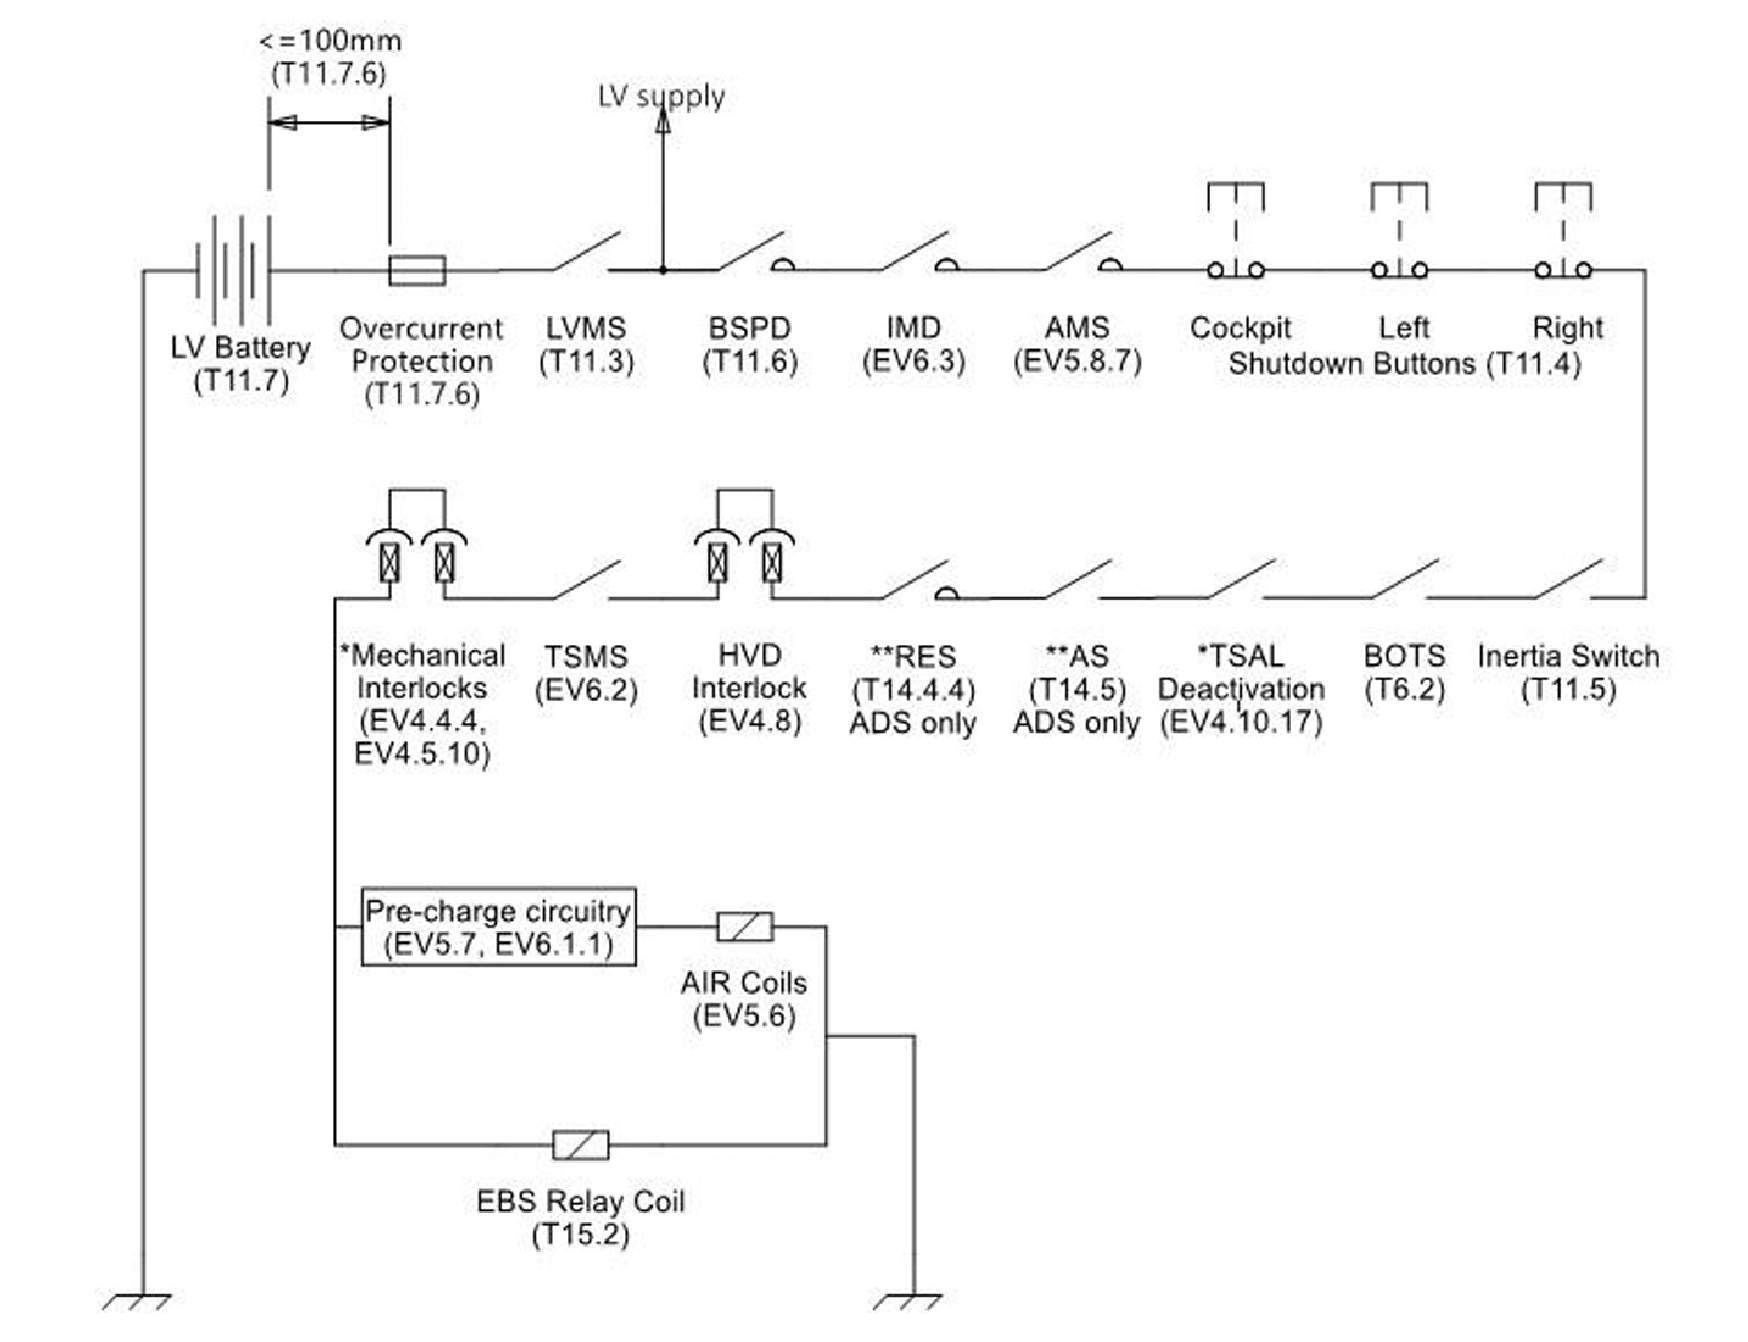
\includegraphics[width=\linewidth]{shutdown_circuit.png}
    \caption{ Shutdown Circuit Design\cite{fs-ev-rules2026}
    }
    \label{fig:shutdown_circuit_design}
\end{figure}

This series configuration ensures that a fault in any individual component will activate the entire circuit, resulting in immediate shutdown by Accumulator Isolation Relays(AIRs).

In addition, the circuit is designed such that any loss of power or disconnection will also result in the shutdown circuit opening, ensuring inherently fail-safe behaviour.

\subsection{Key Components and Operation}

The shutdown circuit consists of a series of safety-critical components, including monitoring devices and manual shutdown interfaces.

Key elements include the Accumulator Management System (AMS), Insulation Monitoring Device (IMD), Brake System Plausibility Device (BSPD), and shutdown buttons.

Among these, the Accumulator Isolation Relays (AIRs) act as the final switching elements of the shutdown circuit. When the SDC is closed, the AIR coils are energised, allowing the high-voltage system to remain connected.

%Air Pic maybe

When any fault condition is detected and the SDC is opened, the AIR coils are de-energised, immediately disconnecting the tractive system.

This ensures that all fault conditions, regardless of their origin, result in a direct and reliable shutdown of the high-voltage system.

\section{Drivetrain Design}

\subsection{Design Overview}

The drivetrain system is responsible for transmitting torque from the motor to the driven wheels. A chain drive configuration is selected due to its simplicity, low mass, and suitability for short-duration acceleration applications, where efficiency and lightweight design are prioritised.

A typical chain-drive drivetrain consists of a driving and driven sprocket connected by a chain. For the selected YASA P400R motor, which does not include an integrated output shaft, a custom shaft is designed to connect the motor to the drivetrain.

The transmission ratio is determined from simulation, with a final drive ratio of 5.5:1 selected to balance torque and speed for the acceleration event. Lightweight materials are used to minimise system mass while maintaining sufficient strength.

%maybe sprocket size? (ask Michael)

\subsection{Material Selection}

Material selection is performed using a strength-to-weight approach. An Ashby plot of material strength versus density is used to compare candidate materials.

Materials with high strength-to-weight ratios are preferred to minimise mass while maintaining structural integrity.

Due to different loading conditions, different materials are selected for specific components. The output shaft, which is subjected to higher torsional loads, is manufactured using glass fibre reinforced polymer (GFRP) to provide sufficient strength while maintaining low weight.

For the chain and sprocket components, where the loading is comparatively lower, nylon~6 is selected due to its lightweight properties and adequate mechanical performance.

In addition, practical considerations such as cost, reliability, and manufacturability are taken into account to ensure feasibility.

\section{Differential Design}

\subsection{Design Rationale}

For a straight-line acceleration application, a differential is not strictly required, as both driven wheels can be powered equally.

However, system-level considerations show that incorporating a differential enables a centralised braking configuration. Replacing two wheel-mounted braking systems with a single centralised braking system reduces the overall system mass, despite the addition of the differential.
% Michael's new table to replace this one - citation
\subsection{Configuration Comparison}

\begin{table}[H]
\centering
\caption{Comparison of Drivetrain Configurations (based on Breaking system analysis from Ziyang Xing)}
\label{tab:drivetrain_comparison}
\begin{tabular}{lcccc}
\toprule
Configuration & Component & Quantity & Weight per Unit (kg) & Total Weight (kg) \\
\midrule
\multirow{4}{*}{Without Differential}
& Braking System & 2 & 1.8 & 3.6 \\
& Upright & 2 & 1.2 & 2.4 \\
& Differential & 0 & -- & 0 \\
& Total & & & \textbf{6}\\
\midrule
\multirow{4}{*}{With Differential} 
& Braking System & 1 & 1.8 & 1.8 \\
& Upright & 1 & 0.8 & 0.8 \\
& Differential & 1 & 2.5 & 2.5 \\
& Total & & & \textbf{5.1} \\
\bottomrule
\end{tabular}
\end{table}

The results indicate that the configuration with a differential achieves a lower total system mass.

\subsection{Differential Selection}

The differential is selected based on minimising weight and cost while ensuring sufficient torque capacity.

A comparison of candidate options shows that the Drexler FSAE LSD \cite{Drexler_FSAE_LSD_data_sheet}
achieves the highest overall score due to its low mass and adequate torque capability. Therefore, it is selected as the most suitable differential for the drivetrain system.

\section{Summary}

The powertrain system is designed to maximise acceleration performance under the constraints of the Formula Student UK\cite{fs-ev-rules2026}.
%how to say FSUK, everyone should say the same

A centralised single-motor architecture is selected to reduce system complexity and mass. The YASA P400R motor is chosen based on its superior torque performance and compatibility with the electrical system.

The inverter selection prioritises voltage range to accommodate the variable output of the supercapacitor system, resulting in the selection of the BAMOCAR PG-D3-700/400.

A structured control system is developed to ensure stable operation, incorporating signal processing, plausibility checks, and constraint handling. Safety is ensured through a shutdown circuit designed in accordance with FSUK requirements.

In addition, system-level optimisation is applied to the mechanical design. A lightweight drivetrain is implemented with a custom output shaft and material selection based on strength-to-weight considerations.

The inclusion of a differential enables a centralised braking configuration, reducing overall system mass.

Overall, the design demonstrates an integrated approach that balances performance, safety, and practicality, resulting in an efficient and competitive powertrain system.
\vspace{1cm}
%maybe add some system images here
%maybe add final parameters here

\compactbib
% --- END INLINE: Yuze Jiang/Engineering/main.tex ---
\end{refsection}

\begin{refsection}
\graphicspath{{../PaulVogelberg/Engineering/}}
% --- BEGIN INLINE: PaulVogelberg/Engineering/paul_body.tex ---
\chapterauthor{Accumulator Design}{Paul Vogelberg}

\section{Introduction}
This chapter presents the accumulator design for the FS vehicle. Objectives are to deliver short-term energy and high power for the acceleration event while minimising mass and packaging volume, complying with scrutineering and electrical safety requirements, and integrating with the vehicle.

The chapter is structured as follows: Section~\ref{sec:technology_selection} covers technology selection; Section~\ref{sec:electrical_system_design} covers electrical design; Section~\ref{sec:mechanical_design_packaging} covers mechanical packaging; Section~\ref{sec:results_discussion} presents results; and Section~\ref{sec:future_improvements_conclusion} outlines future work and concludes.

This chapter covers technology and cell selection; electrical architecture at pack and segment level; in-casing electrical safety measures required by the Formula Student rules; the AMS slave-to-master monitoring architecture and its interface to the vehicle ECU; mechanical packaging of segment modules and accumulator container layout; and analytical verification against requirements and key alternatives.

Safety and charging systems outside the accumulator casing, full AMS firmware implementation, detailed manufacturing process planning, exhaustive scrutineering documentation, and complete physical test campaign data are treated as out of scope.

\section{Technology Selection}
\label{sec:technology_selection}

\subsection{Design Requirements and Selection Criteria}
Due to the nature of the acceleration-only event, the primary design driver is peak power delivery rather than total energy capacity. This shifts the focus towards technologies with high power density.

To compare energy storage technologies, the following criteria were defined: (1) power output, (2) total energy capacity, and (3) a combined optimisation objective covering mass, volume, cost, and procurement risk.
FS rules limit tractive system (TS) power at the tractive system accumulator (TSAC) outlet to 80 kW (FS-EV~2.2.1). Power is treated as constant for an initial conservative energy estimate, assuming traction-limited periods are brief relative to total run time. Event duration is set to \SI{4}{\second}, based on top Formula Student performances of \SI{3.5}{\second}.

The required energy capacity is calculated as:
\begin{equation*}
E = P \cdot t = 80~\text{kW} \times 4~\text{s} = 320~\text{kJ} = 89~\text{Wh}
\end{equation*}

The resulting design requirements used for downstream verification are defined in Table~\ref{tab:design_requirement_ids}.

\begin{table}[htbp]
    \centering
    \caption{Requirement table with targets for the accumulator design.}
    \label{tab:design_requirement_ids}
    \footnotesize
    \begin{tabular}{|c|l|l|}
        \hline
        \textbf{ID} & \textbf{Requirement} & \textbf{Target} \\
        \hline
        R1 & Peak power capability & $= 80\,\text{kW}$ \\
        R2 & Usable event energy & $\geq 320\,\text{kJ}$\\
        R3 & Minimise mass, volume, cost, and procurement risk & Less than best alternative \\
        \hline
    \end{tabular}
\end{table}

\subsection{Energy Storage Media Survey}

\begin{table}[htbp]
    \centering
    \caption{Comparative performance of electrochemical energy storage technologies. Values represent commercially available cell ranges \cite{kalaiarasi2024tale}. Minimum mass calculated for 80 kW power and 89 Wh energy requirements.}
    \label{tab:storage_comparison}
    \footnotesize
    \begin{tabular}{|l|c|c|l|c|l|}
        \hline
        \textbf{Technology} & \makecell{\textbf{Power} \\ \textbf{Density} \\ \textbf{(kW/kg)}} & \makecell{\textbf{Energy} \\ \textbf{Density} \\ \textbf{(Wh/kg)}} & \makecell{\textbf{Limiting} \\ \textbf{Density}} & \makecell{\textbf{Min.} \\ \textbf{Mass} \\ \textbf{(kg)}} & \textbf{Availability} \\
        \hline
        Symmetric SC & ~9 & 3 -- 5 & Energy & 17.8 & Commercially available \\
        Asymmetric / Hybrid SC & 4 -- 5 & 30 -- 100 & Power & 16 & In research phase \\
        Lithium (Pouch) Battery & 1 -- 3 & 120 -- 190 & Power & 26.7 & Commercially available \\
        \hline
    \end{tabular}
\end{table}

Table~\ref{tab:storage_comparison} summarises representative power and energy densities of the best 3 candidates for our solution. Technologies have been shortlisted by minimum mass for the required power and energy.

Other accumulator technologies in the table were considered, but not shown since these had even lower power densities than lithium batteries and therefore were not competitive.
Using this metric, asymmetric / hybrid supercapacitors are best; however, they are excluded further from consideration due to being in the research phase \cite{kalaiarasi2024tale}, leading to limited commercial availability and specification data to ground the design around. The focus is therefore on comparing symmetric supercapacitors and high-power Lithium-ion Polymer (LiPo) batteries, with the former expected to have a significant mass advantage due to superior power density.

\subsection{Supercapacitor Analysis}
\label{subsec:supercapacitor_analysis}

Supercapacitors are treated as the primary candidate, with LiPo cells used as a benchmark. Electric Double Layer Capacitor (EDLC) devices are selected within the symmetric supercapacitor class due to relatively high energy capacity. Energy for capacitors is given by:
\begingroup
\setlength{\abovedisplayskip}{8pt plus 0pt minus 0pt}
\setlength{\belowdisplayskip}{8pt plus 0pt minus 0pt}
\setlength{\abovedisplayshortskip}{8pt plus 0pt minus 0pt}
\setlength{\belowdisplayshortskip}{8pt plus 0pt minus 0pt}
\begin{equation}
E=\frac{1}{2}CV^2 = \frac{1}{2} C (V_{max}^2-V_{min}^2)
\label{eq:capacitor_energy}
\end{equation}
\endgroup

where $E$ is energy (J), $C$ is capacitance (F), and $V$ is voltage (V).

From Equation \eqref{eq:capacitor_energy}, voltage sag significantly affects usable energy capacity, necessitating careful consideration of voltage ranges. The upper limit is set by FS-EV maximum voltage regulation (600\,V per FS-EV~4.1.1), while the lower limit is determined by inverter and motor minimum operating requirements. The powertrain operating strategy in Section~\ref{subsec:powertrain_motor_operation} indicates the motor can be controlled under the power cap with an effective operating voltage on the order of \SI{350}{\volt}, so \SI{400}{\volt} is adopted here as a conservative design minimum.
\begingroup
\setlength{\abovedisplayskip}{8pt plus 0pt minus 0pt}
\setlength{\belowdisplayskip}{8pt plus 0pt minus 0pt}
\setlength{\abovedisplayshortskip}{8pt plus 0pt minus 0pt}
\setlength{\belowdisplayshortskip}{8pt plus 0pt minus 0pt}
\begin{equation}
C=\frac{2 E}{V_{max}^2-V_{min}^2}=\frac{2 \cdot 320\text{ kJ}}{600\text{ V}^2-400\text{ V}^2}=3.2\text{ F}
\label{eq:required_capacitance}
\end{equation}
\endgroup

To achieve the required capacitance of 3.2 F at 600 V, cells are connected in series. The general relation for non-identical cells reduces to the equally rated case as:
\begingroup
\setlength{\abovedisplayskip}{8pt plus 0pt minus 0pt}
\setlength{\belowdisplayskip}{8pt plus 0pt minus 0pt}
\setlength{\abovedisplayshortskip}{8pt plus 0pt minus 0pt}
\setlength{\belowdisplayshortskip}{8pt plus 0pt minus 0pt}
\begin{equation}
\frac{1}{C_{total}} = \sum_{i=1}^{n} \frac{1}{C_{i}}\;\Rightarrow\;C_{series}=\frac{C_{i}}{n}
\label{eq:series_capacitance}
\end{equation}
\endgroup

where \(C_i\) is the individual cell capacitance, and n is the number of cells in series.

For the design specification, assuming a cell voltage of 3 V, 200 cells are required in series to reach 600 V. To achieve the required capacitance of 3.2 F, cells must provide 640 F capacitance.

Another key parameter is the Equivalent Series Resistance (ESR), which becomes an important consideration for series-connected supercapacitor cells. The voltage evolution during constant-power discharge is modelled via the following first-order differential equation:
\begingroup
\setlength{\abovedisplayskip}{8pt plus 0pt minus 0pt}
\setlength{\belowdisplayskip}{8pt plus 0pt minus 0pt}
\setlength{\abovedisplayshortskip}{8pt plus 0pt minus 0pt}
\setlength{\belowdisplayshortskip}{8pt plus 0pt minus 0pt}
\begin{equation}
\frac{dV}{dt} = -\frac{P}{C \cdot V} - \frac{P^2 \cdot R_{total}}{C \cdot V^3}
\label{eq:pack_voltage_dynamics}
\end{equation}
\endgroup

Where $V(t)$ is the instantaneous pack voltage, $P$ is the constant power draw (W), $C$ is the pack capacitance (F), and $R_{total} = ESR_{cell} \times n$ is the total series resistance (\(\Omega\)) with $ESR_{cell}$ the individual cell ESR and $n$ the number of cells in series. The first term represents capacitive voltage decay; the second term represents resistive voltage loss proportional to $I^2 R$ dissipation.

\subsection{Supercapacitor Cell Selection}
\begin{table}[htbp]
    \centering
    \caption{Supercapacitor cell comparison with constants for all candidates: cell capacitance $C_i=600\,\text{F}$, cell voltage $V_{cell}=3.0\,\text{V}$, giving total series capacitance $C_{total}=3.0\,\text{F}$ (Eq.~\ref{eq:series_capacitance}) with $n=200$. Min. Voltage \& Max. Current calculated using $P=80\,\text{kW}$ sustained for 4s.}
    \label{tab:supercap_cells}
    \begin{tabular}{|c|l|c|c|c|c|c|}
        \hline
        \textbf{ID} & \textbf{Part Number} & \textbf{ESR} & \makecell{\textbf{Cell} \\ \textbf{Mass}} & \makecell{\textbf{Total} \\ \textbf{Mass}} & \makecell{\textbf{Min. Voltage} \\ \textbf{(Eq.~\ref{eq:pack_voltage_dynamics})}} & \makecell{\textbf{Max Current} \\ \textbf{(P/V\textsubscript{min})}} \\
        & & \textbf{(m$\Omega$)} & \textbf{(kg)} & \textbf{(kg)} & \textbf{(V)} & \textbf{(A)} \\
        \hline
        SC1 & C46W-3R0-0600 \cite{sech-c46w-3r0-0600} & 0.70 & 0.139 & 27.8 & 369.2 & 216.6 \\
        SC2 & C35S-3R0-0600 \cite{gmcc-c35s-3r0-0600} & 1.40 & 0.104 & 20.8 & 354.1 & 226.0 \\
        SC3 & CHQ-3R0607R-TW \cite{cda-chq-3r0607r-tw} & 1.30 & 0.135 & 27.0 & 356.3 & 224.6 \\
        \hline
    \end{tabular}
\end{table}

Initial evaluation favored SC3 (Table \ref{tab:supercap_cells}), which offered a good balance between mass and required capacitance while facilitating easy segmentation with its standard 3 V cell voltage. However, further supplier investigation revealed SC2 as a lower-mass alternative. Ultimately, SC1 was selected due to its significantly lower ESR, which minimises voltage sag during the acceleration event, despite a mass penalty relative to other candidates.

\begin{figure}[htbp]
    \centering
    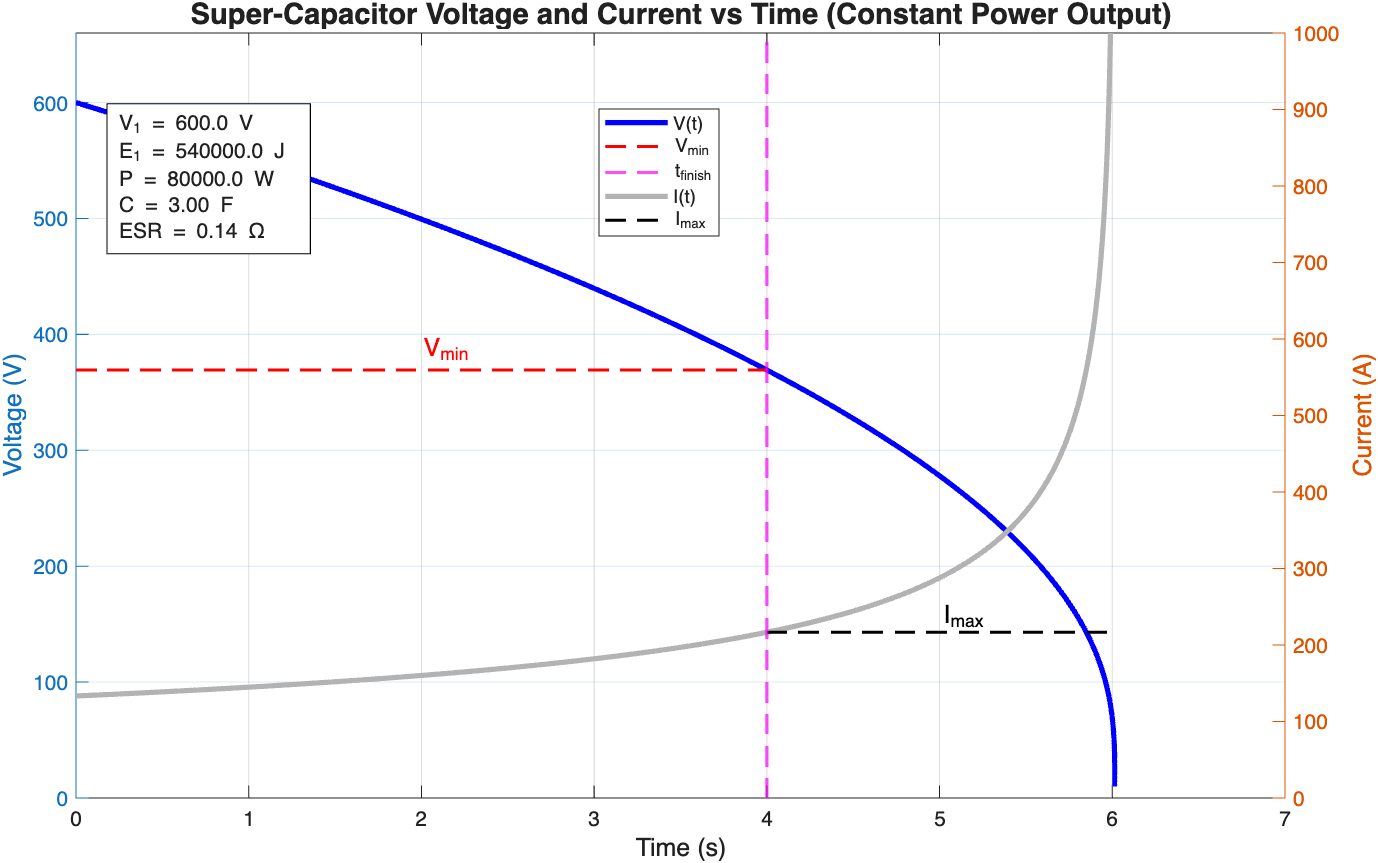
\includegraphics[width=1\textwidth]{figures/Supercapcaitor_discharge.png}
    \caption{Selected supercapacitor (SC1) discharge characteristics showing voltage and current evolution over time during constant 80 kW power discharge.}
    \label{fig:supercap_discharge}
\end{figure}

Figure \ref{fig:supercap_discharge} shows the voltage and current evolution during a constant 80 kW power discharge, giving a conservative estimate. The voltage starts at 600 V and drops to 369 V at the end of the event, set by $t_{finish}=4\,\text{s}$, confirming the expected voltage sag due to both capacitive discharge and resistive losses. The current increases to 217 A, acceptable thermally for short bursts.

\subsection{Tolerance Analysis}

The supercapacitor datasheet gives a capacitance tolerance of +0--20\% (typically +5--10\%). This tolerance dominates cell-to-cell capacitance mismatch in a series string, which drives the required passive balancing duty; binning can reduce mismatch and therefore reduce balancing demand (see Section~\ref{subsec:electrical_design}).

Cells are supplied in packs of 90, requiring purchase of three packs and selection of the best 200 cells. For this event, selection is simplified to maximising capacitance rather than minimising variance because balancing heat is not expected to be the limiting factor.

The cell capacitances are modelled using a beta distribution:
\begin{equation*}
T = 0.2*Beta(\alpha = 3, \beta = 5)
\end{equation*}

Selecting the highest cells, the expected accumulator capacitance is calculated using Equation~\eqref{eq:series_capacitance}.

Performing this Monte Carlo binning simulation to find average mean total capacitance and capacitance range gives the improvements summarised in Table~\ref{tab:capacitance_binning_results}.

\begin{table}[htbp]
    \centering
    \caption{Accumulator performance comparison for nominal and binned (average) capacitance scenarios. Relative differences are reported against the nominal case. Constants: $P_{const}=80\,\mathrm{kW}$, $V_{total}=600\,\mathrm{V}$, $t_{finish}=4\,\mathrm{s}$, $R_{total}=0.14\,\Omega$.}
    \label{tab:capacitance_binning_results}
    \footnotesize
    \begin{tabular}{|l|c|c|c|}
        \hline
        \textbf{Metric} & \textbf{Nominal} & \textbf{Binned} & \textbf{Difference} \\
        \hline
        Capacitance (F) & 3.00 & 3.26 & +8.7\% \\
        Initial Energy (kJ) & 540 & 587 & +8.7\% \\
        Minimum Voltage (V) & 369 & 393 & +6.6\% \\
        Maximum Current (A) & 217 & 203 & -6.2\% \\
        Capacitance Range & 0\% & 10\% & \\
        \hline
    \end{tabular}
\end{table}

\subsection{Technology Selection Decision}

The two remaining candidates (EDLC and LiPo) are compared on mass, volume, cost, electrical performance, availability and complexity. High-power LiPo remains the benchmark because it is widely used in Formula Student. Comparison proceeds via quantifiable metrics of mass and volume. Cost cannot be quantified accurately due to the ambiguity in pricing for LiPo cells. Electrical performance should be similar if our criteria are met, whilst availability and complexity will be considered later as qualitative factors.


\begin{table}[htbp]
    \centering
    \caption{Comparison of EDLC supercapacitor and high-power LiPo battery technologies \cite{batpac2022manual}. Weighted scoring system applied. LiPo wins by 4.0\% overall score, driven by volume advantages.}
    \label{tab:tech_comparison}
    \footnotesize
    \begin{tabular}{|l|c|c|l|}
        \hline
        \textbf{Technology} & \makecell{\textbf{Mass*} \\ \textbf{(kg)}} & \makecell{\textbf{Cell Volume} \\ \textbf{(L)}} & \textbf{Evaluation Method} \\
        \hline
        EDLC Cap. & 29.8 & 22.4 & Bottom-Up Estimate \\
        \arrayrulecolor{gray!30}\hline\arrayrulecolor{black}
        LiPo Battery & 33.1 & 12.5 & Top-Down Estimate \\
        \hline
        \hline
        \multicolumn{4}{|c|}{\textbf{Weighted Scoring Analysis}} \\
        \hline
        \textbf{Technology} & \textbf{Mass (3×)} & \textbf{Volume (1×)} & \textbf{Total Score} \\
        \hline
        EDLC & 3.00 & 0.56 & 3.56 \\
        \arrayrulecolor{gray!30}\hline\arrayrulecolor{black}
        LiPo & 2.70 & 1.00 & 3.70 \\
        \hline
        \textbf{Best} & \textbf{EDLC} & \textbf{LiPo} & \cellcolor{green!20}\textbf{LiPo} \\
        \hline
        \multicolumn{3}{|r|}{\textbf{LiPo Advantage:}} & \textbf{+4.0\%} \\
        \hline
    \end{tabular}
\end{table}

Two different methodologies are used to estimate mass and volume for the two technologies. For LiPo, the top-down BatPac simulation tool \cite{batpac2022manual} determines a mass-sensitive pack design. Inputs characterise both the FS regulations and the acceleration focus whilst retaining physical accuracy. An asterisk is placed next to mass in the table, as this is not total mass (which cannot yet be determined) but the sum of cell mass and other technology-specific masses. For LiPo this includes heavier pack hardware and thermal management, whilst for SC only lighter pack hardware weight is included. The supercapacitor cell mass and volume are calculated using a bottom-up approach based on the selected cell (SC1) specifications \cite{sech-c46w-3r0-0600}. Whilst LiPo pouch cells can be more tightly packed than cylindrical SC cells, they require more mechanical support, so cell volume is an accurate relative indicator of total volume for this comparison.

A weighted scoring system is applied using the following formulation:
\begingroup
\setlength{\abovedisplayskip}{8pt plus 0pt minus 0pt}
\setlength{\belowdisplayskip}{8pt plus 0pt minus 0pt}
\setlength{\abovedisplayshortskip}{8pt plus 0pt minus 0pt}
\setlength{\belowdisplayshortskip}{8pt plus 0pt minus 0pt}
\begin{equation*}
\text{Score} = \frac{\text{Best Value in Category}}{\text{Component Value}} \cdot \text{Weight}
\end{equation*}
\endgroup

A 70-30 weighting is typically applied for mass and volume, as mass has a higher impact on performance. Volume's biggest impact is the increased aerodynamic drag which it introduces. However, for this acceleration-only application, where initial speeds are low, this has a less significant effect, hence the weightings have been adjusted to 75-25 (or 3-1) to reflect this appropriately.

Whilst LiPo is advantageous in our weighted scoring analysis, it does not consider qualitative factors. The increased complexity of chemical cells introduces additional safety and thermal management challenges. In addition, availability and pricing uncertainty introduce risk to the project timeline and budget. Hence, SCs were selected, as the minor quantitative advantages of LiPo do not justify these qualitative disadvantages.

\section{Electrical System Design}
\label{sec:electrical_system_design}

\subsection{System Architecture Overview}

Figure~\ref{fig:electronics_architecture} shows the top-level accumulator architecture. This section is structured from power-path implementation to supervisory control: busbar design, safety design, monitoring and control, and finally system integration. The architecture consists of five high-voltage (HV) segments, each monitored by AMS slaves (MC33771 \cite{nxp-mc33771-ds}), communicating with the AMS master (FRDM33664BEVB \cite{nxp-frdm33664bevb-ug}) via the MC33664 Twisted Pair Link (TPL) interface \cite{nxp-mc33664-ds}. The low-voltage (LV) control domain interfaces to the vehicle ECU (STM32 Nucleo-F4 \cite{stm32-nucleo-f4}) over CAN, using the SN65HVD230 transceiver \cite{ti-sn65hvd230-ds}. Additional key components include Bussmann 170M1759 fusing at inter-segment \cite{eaton-bussmann-170m1759-ds}, and an EarthX ETX12A 12 V supply battery \cite{earthx-etx12a-ds}. External charging and vehicle shutdown-chain implementation are outside the scope of this section.

\begin{figure}[!htbp]
    \centering
    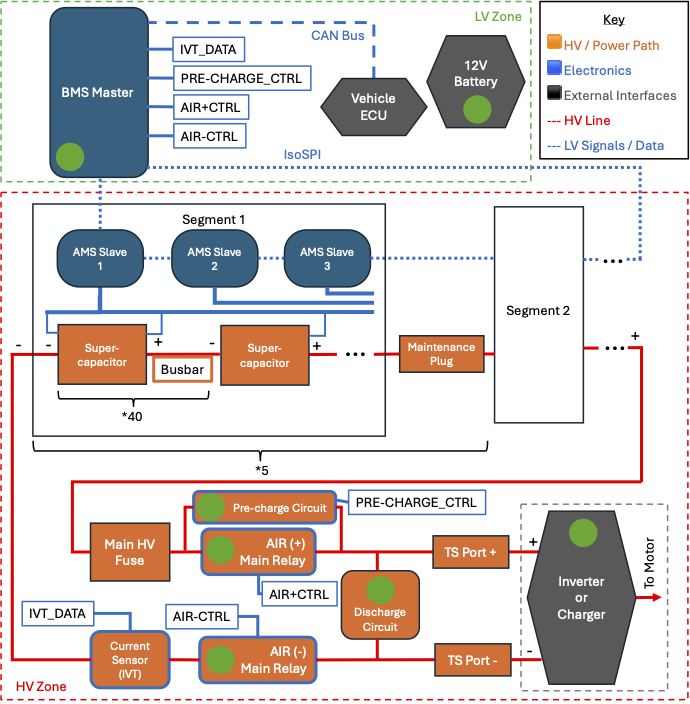
\includegraphics[width=0.95\textwidth]{figures/schematics/Electronics_architecture.png}
    \caption{Top-level electrical system architecture showing energy flow from supercapacitor cells through busbars and segments to the inverter, alongside control and communication pathways within the AMS. Green dots represent the 12 V battery connection.}
    \label{fig:electronics_architecture}
\end{figure}

\subsection{Busbar Design}

Supercapacitors are connected via busbars rather than direct cell-to-cell welding for thermal expansion management and assembly accessibility. Busbar material selection minimises $\rho_{e} \cdot \rho_{m}$, where $\rho_{e}$ is electrical resistivity and $\rho_{m}$ is mass density. Although copper exhibits superior electrical performance, aluminium 1005 was specified for compatibility with aluminium cell terminals.

Busbar connection area is matched to the terminal diameter, $d_{t}$, with average busbar length $L$ and target resistance per connection, $R$. The required thickness is calculated as:

\begingroup
\setlength{\abovedisplayskip}{8pt plus 0pt minus 0pt}
\setlength{\belowdisplayskip}{8pt plus 0pt minus 0pt}
\setlength{\abovedisplayshortskip}{8pt plus 0pt minus 0pt}
\setlength{\belowdisplayshortskip}{8pt plus 0pt minus 0pt}
\begin{equation*}
t = \frac{\rho_{e} L}{R d_{t}} = \frac{\left(2.8 \times 10^{-8}\,\Omega\,\text{m}\right)\left(50 \times 10^{-3}\,\text{m}\right)}{\left(0.1 \times 10^{-3}\,\Omega\right)\left(10 \times 10^{-3}\,\text{m}\right)} = 1.41\,\text{mm} \approx 1.45\,\text{mm} \text{ (standard 15 gauge)}
\end{equation*}
\endgroup

\subsection{Safety Design}

Grounding is treated as a floating HV system with insulation monitoring against chassis (FS-EV~4.3.1). Fuse placement is integrated per segment to localise faults and satisfy FS-EV~3.2.1 and FS-EV~3.2.7. For electromagnetic interference (EMI) robustness and rule-compliant layout practice, communication wiring follows segregated HV/LV routing to satisfy FS-EV~4.3.3 physical separation requirements. Any external AMS master to vehicle ECU or diagnostic connection is implemented with galvanic isolation in accordance with FS-EV~4.3.2. Vehicle-level shutdown-chain implementation, AIR actuation hardware, and charging safety circuitry are outside the scope.

\subsection{Monitoring and Control Systems}
\label{subsec:electrical_design}

\begin{figure}[!htbp]
    \centering
    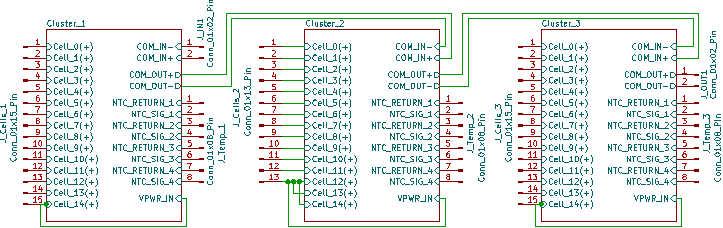
\includegraphics[width=\textwidth]{figures/schematics/PCB.pdf}
    \caption{Complete segment AMS printed circuit board (PCB) schematic showing MC33771 topology for 40-cell segment monitoring.}
    \label{fig:pcb_schematic}
\end{figure}

The controller integrated circuit (IC) is powered directly by the cells themselves via the \texttt{VPWR} pins and therefore floats at the segment potential. The daisy-chain interface follows TPL pin mapping, with \texttt{COM\_IN} receiving data from the lower segment and \texttt{COM\_OUT} forwarding data to the upper segment.

\begin{figure}[!htbp]
    \centering
    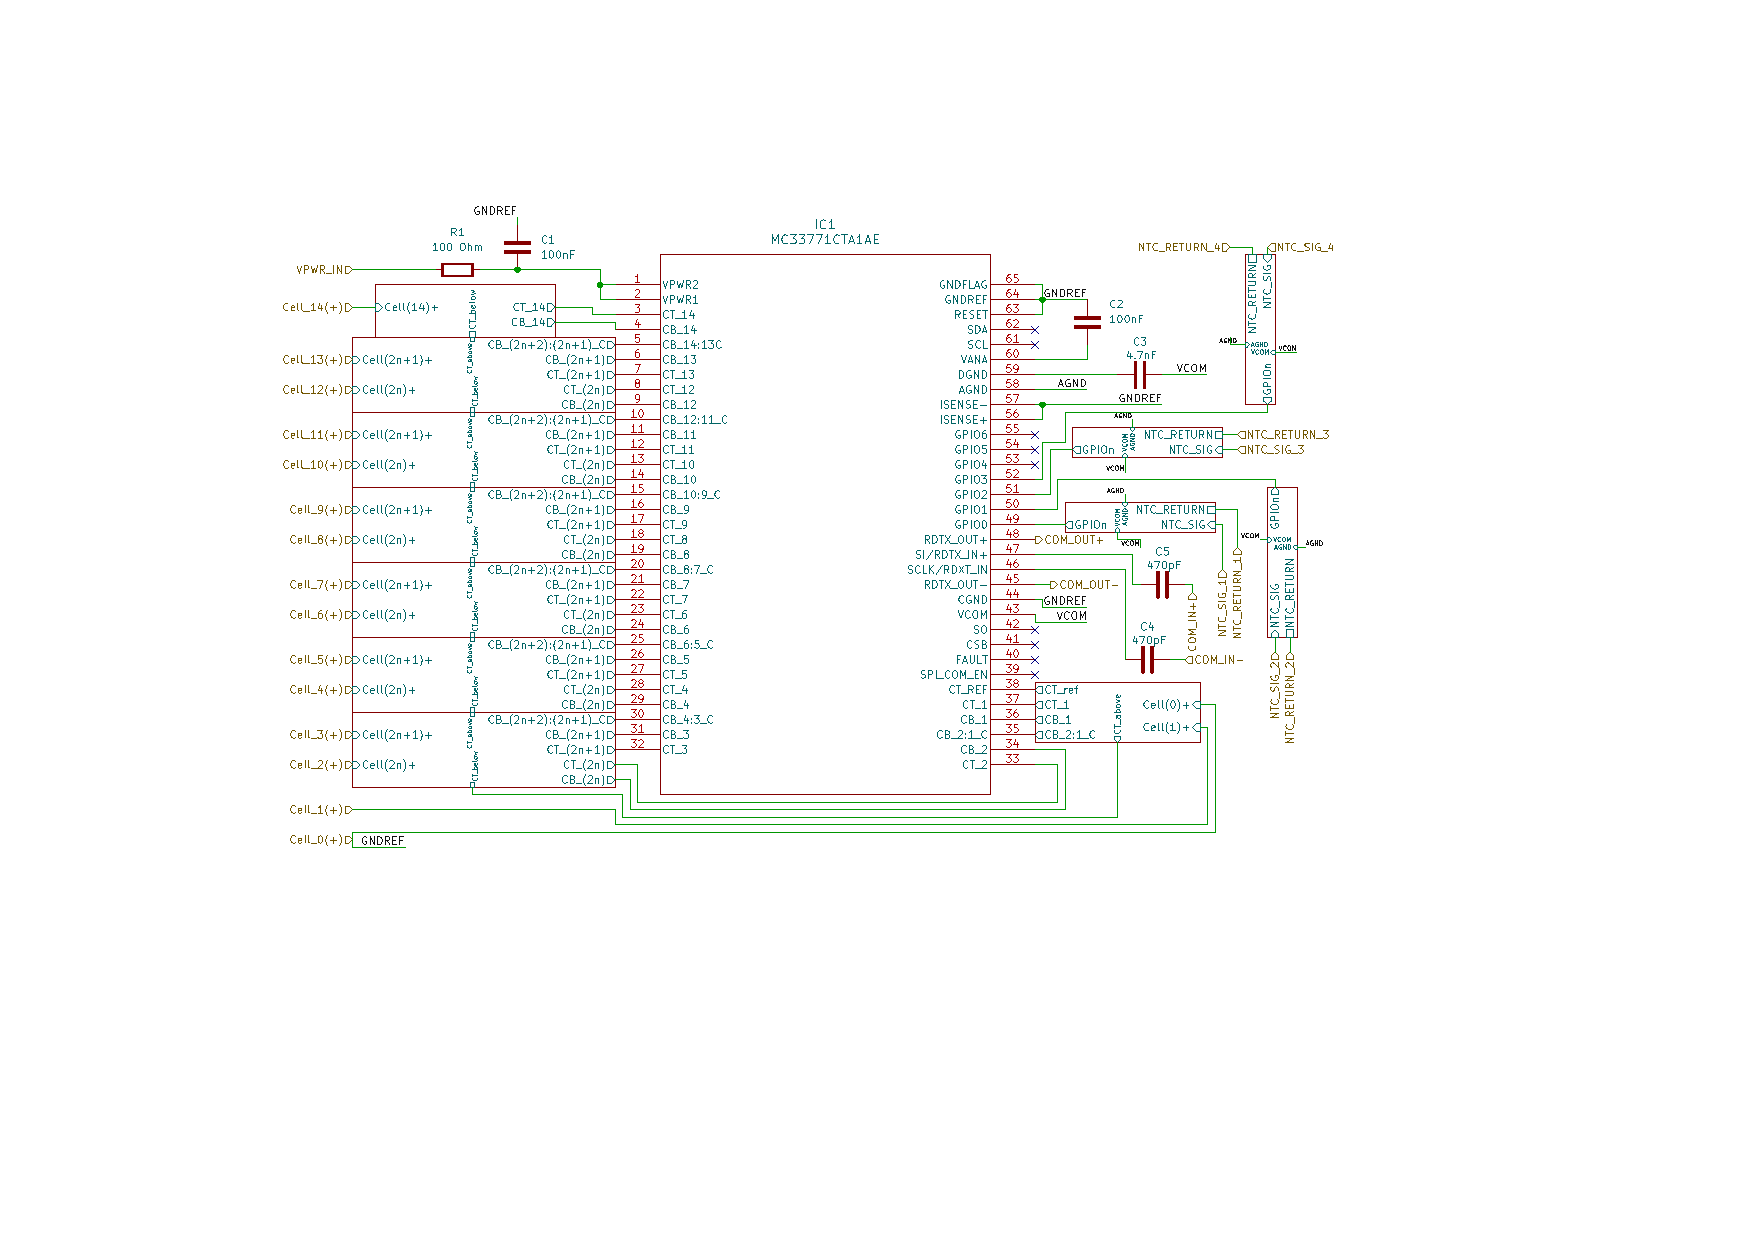
\includegraphics[width=\textwidth]{figures/schematics/PMIC2.pdf}
    \caption{Singular Cluster (1) schematic showing voltage and temperature monitoring with isolation and protection features.}
    \label{fig:pmic}
\end{figure}

\textbf{AMS architecture and communication:} The monitoring network adopts a scalable master-slave topology using NXP MC33771 controllers across five accumulator segments \cite{nxp-mc33771-ds}. Communication is implemented with the NXP TPL interface via the MC33664, whose current-mode transmission provides strong immunity to inverter-generated EMI \cite{nxp-mc33664-ds}. Galvanic domain separation in the daisy chain is maintained using high-voltage safety capacitors ($C4$, $C5$), which couple communication across stacked segment voltage domains while blocking DC transfer.

The TPL bus is implemented as a single-ended daisy chain from the AMS master to the first AMS slave. The architecture uses three AMS slaves per segment across five segments (15 slaves total), with data forwarded stage-by-stage via \texttt{COM\_OUT} to \texttt{COM\_IN}. The end of the chain is terminated using the NXP-recommended end-of-line network, including a termination resistor, to ensure signal integrity and avoid reflections.

Each slave device performs segment voltage and temperature acquisition and reports diagnostic status to the AMS master. The AMS master (FRDM33664BEVB) executes pack-level limit checks, aggregates faults, and communicates accumulator status to the vehicle ECU (STM32 Nucleo-F4).

\textbf{Voltage sensing and balancing:} Cell voltage sensing uses an anti-aliasing resistor-capacitor (RC) filter with $R = 100\,\Omega$ (R6, R7 in Figure~\ref{fig:signal_conditioning}a) and $C = 47\,\text{nF}$ (C8, C9 in Figure~\ref{fig:signal_conditioning}a). The corresponding cutoff frequency:
\begingroup
\setlength{\abovedisplayskip}{8pt plus 0pt minus 0pt}
\setlength{\belowdisplayskip}{8pt plus 0pt minus 0pt}
\setlength{\abovedisplayshortskip}{8pt plus 0pt minus 0pt}
\setlength{\belowdisplayshortskip}{8pt plus 0pt minus 0pt}
\begin{equation*}
f_c = \frac{1}{2\pi R C} = \frac{1}{2\pi (100)(47 \times 10^{-9})} \approx 33.8\,\text{kHz},
\end{equation*}
\endgroup

which attenuates high-frequency inverter switching content while preserving measurement bandwidth for pack diagnostics. Based on the binned-cell capacitance spread of up to 10\% (Table~\ref{tab:capacitance_binning_results}), passive balancing is required to control inter-cell voltage divergence. Passive balancing is implemented through switchable resistors with $R_{bal} = 33\,\Omega$ (R5, R8, R9 in Figure~\ref{fig:signal_conditioning}a). At a nominal maximum cell voltage of 3 V, the corresponding balancing current is $I_{bal} \approx 91\,\text{mA}$, and the dissipation per balancing branch is
\begingroup
\setlength{\abovedisplayskip}{8pt plus 0pt minus 0pt}
\setlength{\belowdisplayskip}{8pt plus 0pt minus 0pt}
\setlength{\abovedisplayshortskip}{8pt plus 0pt minus 0pt}
\setlength{\belowdisplayshortskip}{8pt plus 0pt minus 0pt}
\begin{equation*}
P_{diss} = \frac{V_{cell}^{2}}{R_{bal}} = \frac{(3\,\text{V})^{2}}{33\,\Omega} \approx 0.27\,\text{W}.
\end{equation*}
\endgroup

This thermal load requires resistor packages with sufficient margin, so the format 1210, rated at 0.5\,W, was chosen for stable operation during balancing intervals.

\begin{figure}[!htbp]
    \centering
    \begin{subfigure}[b]{0.65\textwidth}
        \centering
        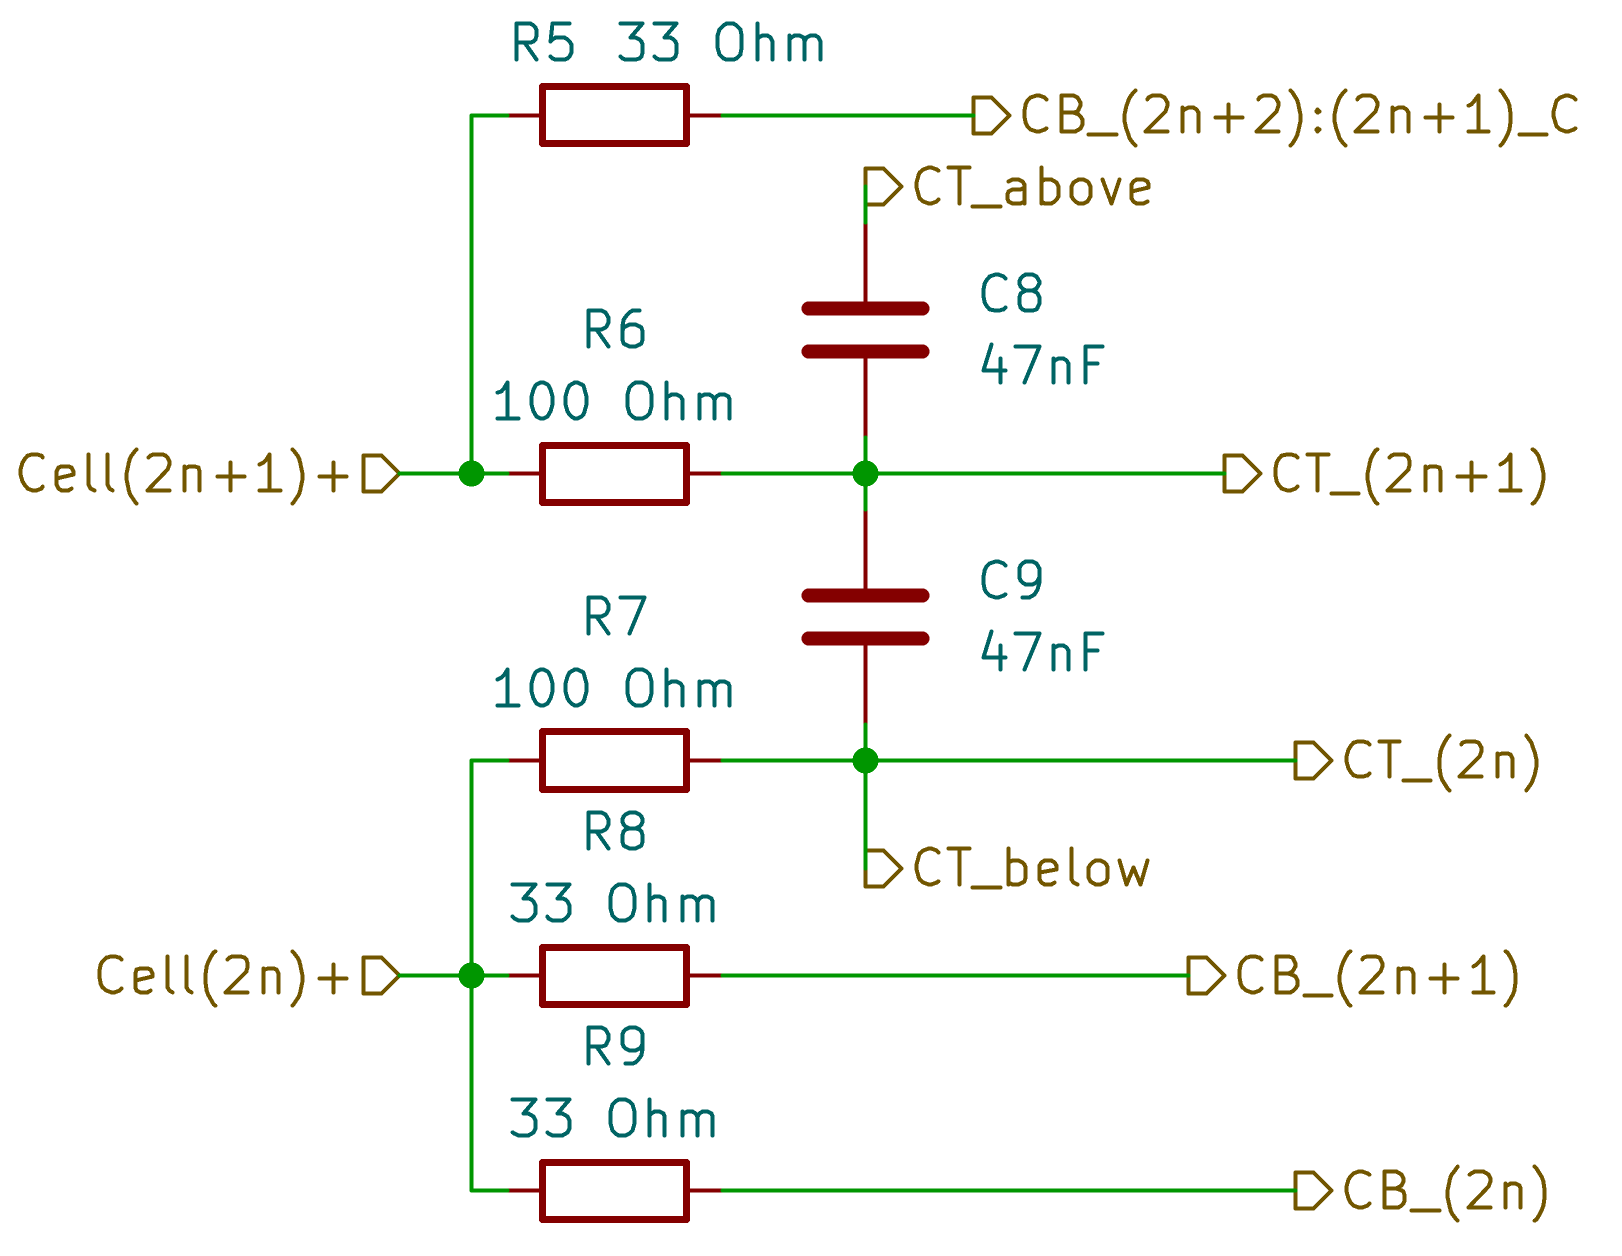
\includegraphics[width=\textwidth]{figures/schematics/VoltageFilter.png}
        \caption{Voltage sensing and filtering circuit.}
        \label{fig:voltage_filter}
    \end{subfigure}
    \hfill
    \begin{subfigure}[b]{0.28\textwidth}
        \centering
        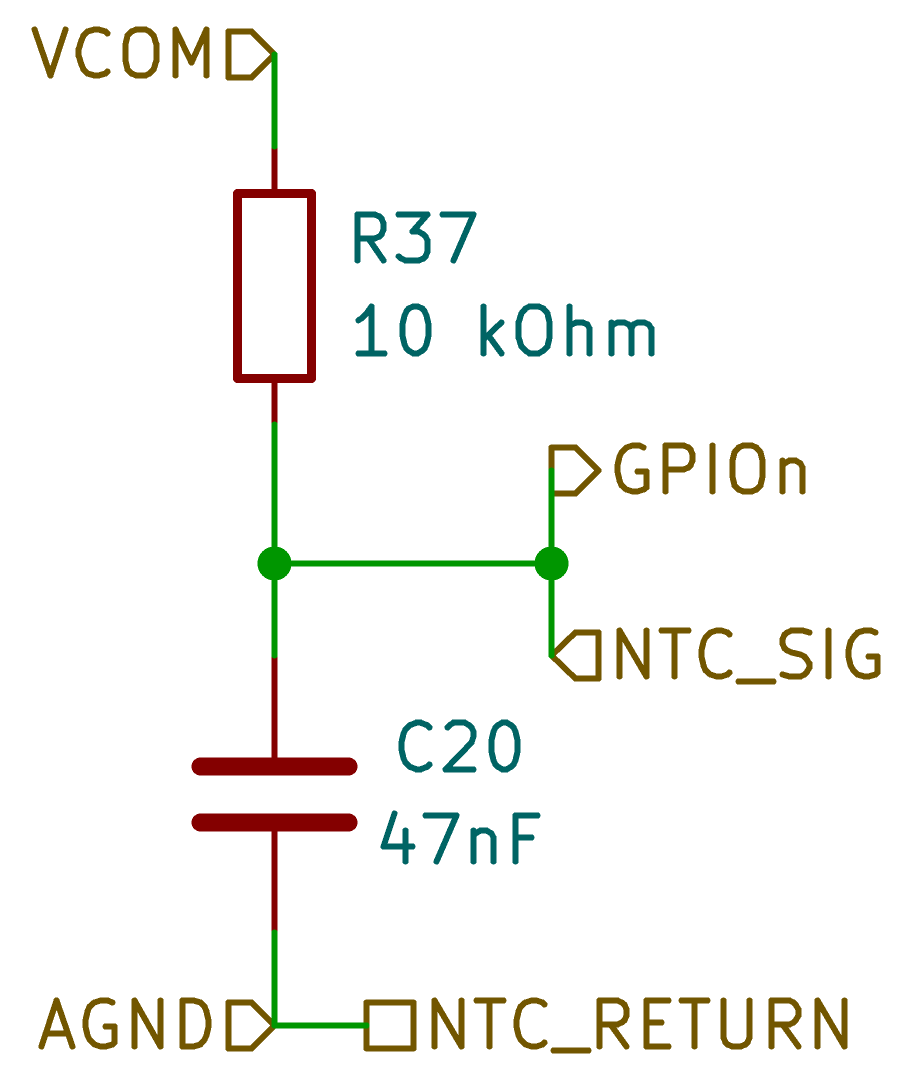
\includegraphics[width=\textwidth]{figures/schematics/TemperatureSensor.png}
        \caption{Temperature sensing circuit.}
        \label{fig:temperature_sensing}
    \end{subfigure}
    \caption{Signal conditioning circuits for AMS monitoring}
    \label{fig:signal_conditioning}
\end{figure}

\textbf{Temperature monitoring and protection:} Temperature channels are conditioned with an RC input filter ($R=10\,\text{k}\Omega$, $C=47\,\text{nF}$), implemented as R37 \& C20 in Figure~\ref{fig:signal_conditioning}b. This suppresses transient noise that could otherwise cause false over-temperature flags. Negative temperature coefficient (NTC) thermistors are connected directly to general-purpose input/output (GPIO) measurement channels, and cell temperature is reconstructed from this voltage. Sensors are placed on 30\% of the cells to satisfy temperature monitoring requirements (FS-EV~5.8.4). The protection strategy applies a hard fault response using the AIR when any monitored cell temperature exceeds $T > 60^\circ\text{C}$ (FS-EV~5.8.5), with AMS-triggered shutdown behavior as required by FS-EV~5.8.7.

\subsection{System Integration}

System integration defines how the accumulator monitoring subsystem interfaces with the rest of the vehicle once local sensing and protection functions are implemented. In this design, the integration point is the AMS master-to-ECU CAN interface, through which pack-level status and fault state should be communicated for vehicle-level decision making.

The AMS master and ECU must operate in the LV domain and should be supplied from the vehicle 12 V system, while all segment electronics should remain referenced to their local HV potentials. Galvanic isolation must be maintained at external interfaces (FS-EV~4.3.2), and TS/LV physical segregation preserved in routing and packaging (FS-EV~4.3.3). Within this report scope, the integration boundary ends at the AMS master to ECU status interface; hence, vehicle shutdown-chain actuation logic, charger-side functions, and full firmware message implementation are not included.

\section{Mechanical Design and Packaging}
\label{sec:mechanical_design_packaging}
The electrical requirement of 200 series-connected cells necessitates segmentation into 5 modules of 40 cells each to maintain voltage domains within FS-EV regulations. All segments are housed within a single Accumulator Container (AC), separated by internal insulating walls.

\subsection{Segment Design}

\begin{figure}[!htbp]
    \centering
    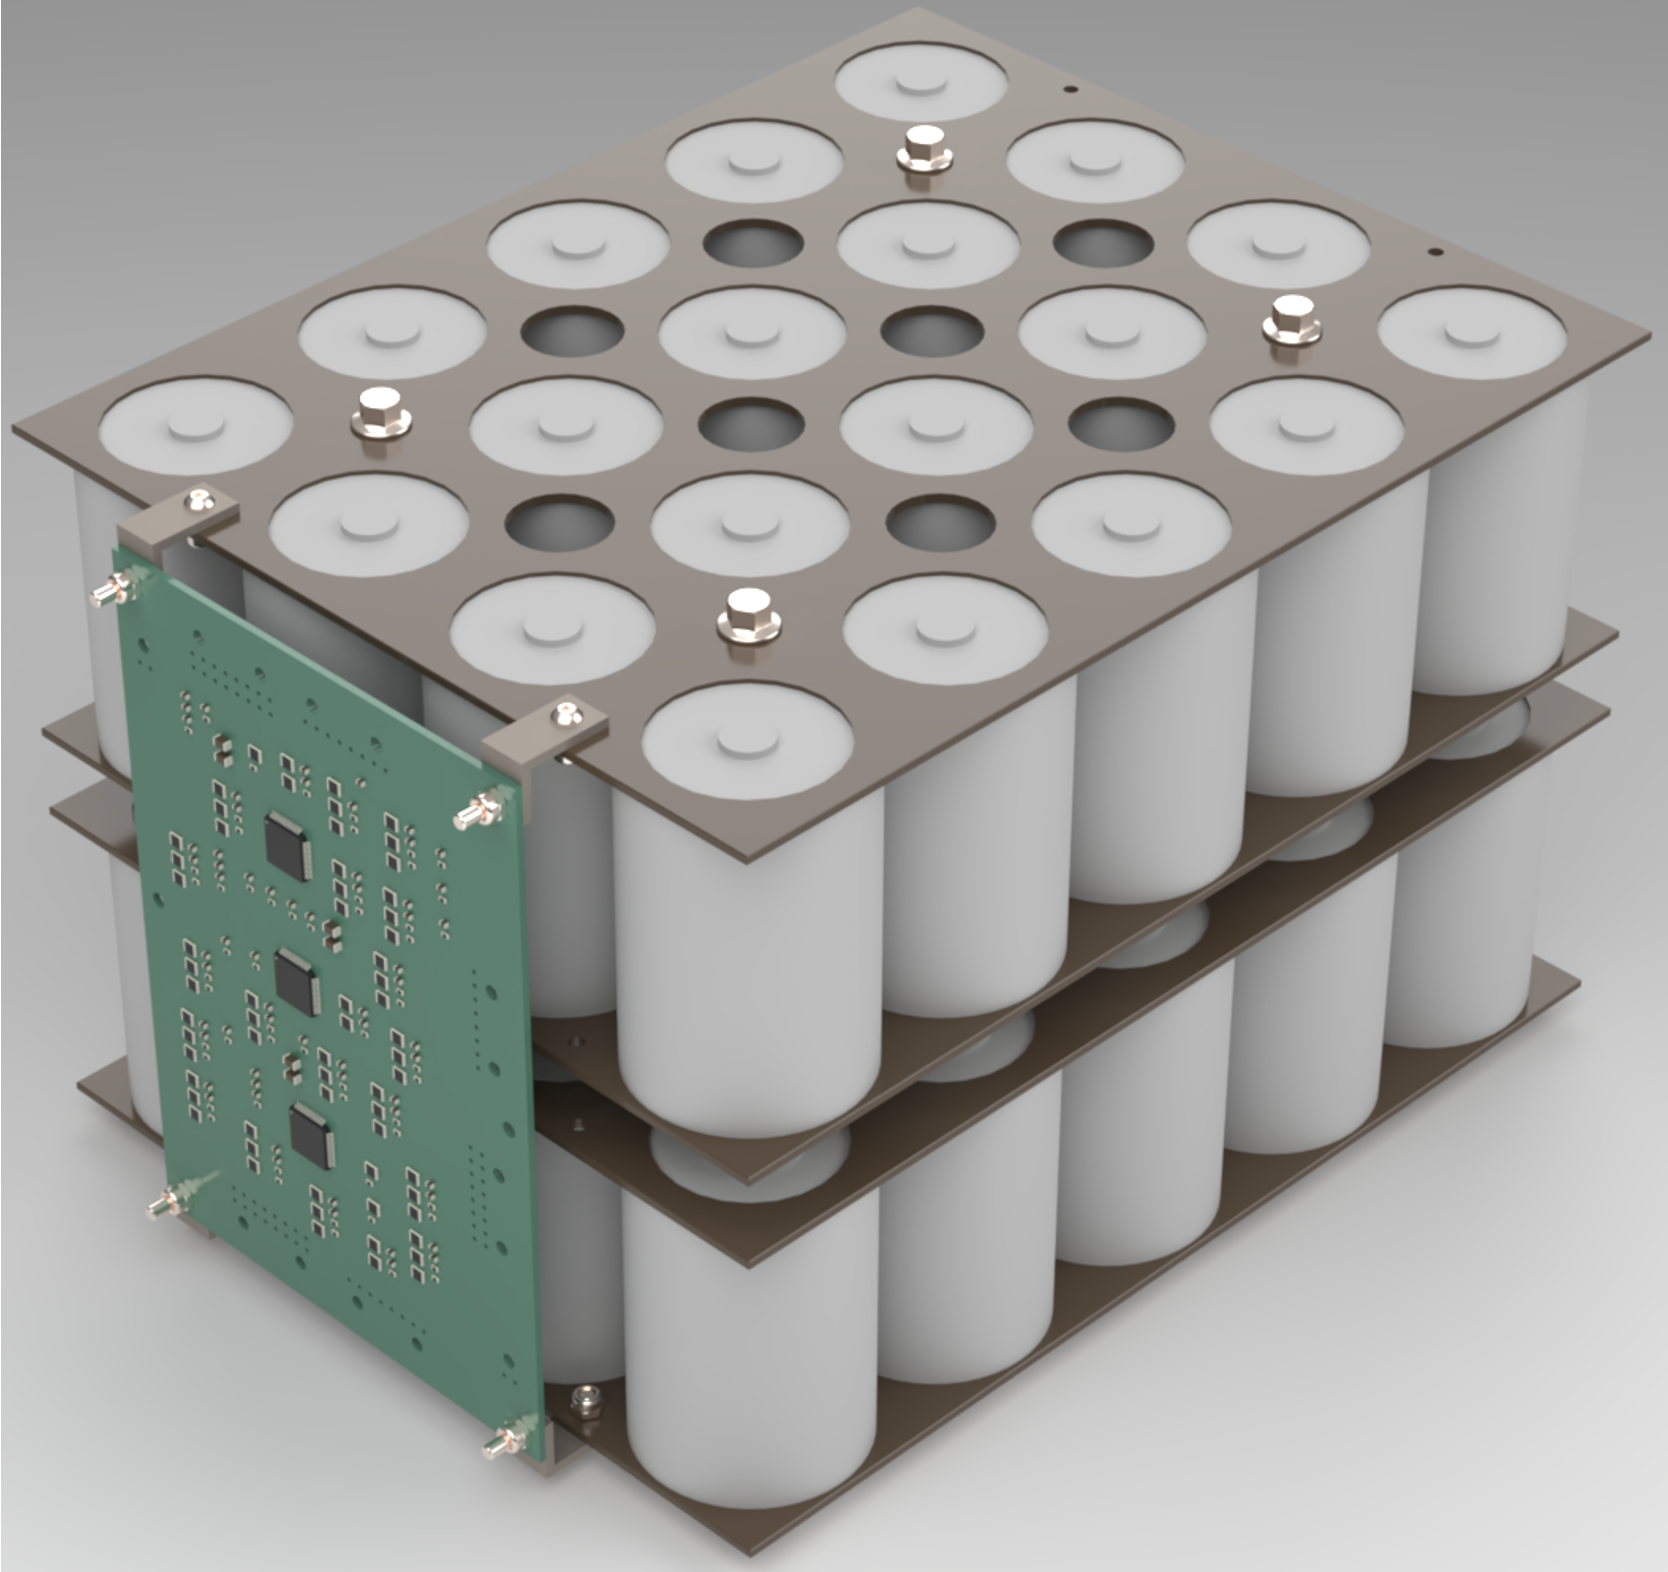
\includegraphics[width=0.9\textwidth]{figures/renders/segment.png}
    \caption{Accumulator segment design without enclosure and busbar connections.}
    \label{fig:main_segment}
\end{figure}

Segment design prioritises modularity and replicability, with each segment containing series-connected cells secured by mechanical holders and electrically isolated by spacing. Each segment comprises two 20-cell sub-modules in a 5×4 rectangular grid, leaving a central corridor for sensing and wiring.

Although honeycomb packing is generally denser, it provides only about 1\% volume reduction once constrained to cuboid envelope, so the rectangular layout is retained for simplicity.

The PCB layout (detailed in Section~\ref{subsec:electrical_design}) is positioned to fit within the segment depth and centred to facilitate harness routing and cell connection while enabling mechanical accessibility via bracket-based mounting to the FR4 (flame-retardant 4) matrix board. PCB peripheral spacing accommodates cable routing.

Fuses are mounted to the casing and their exact position varies by segment because of inter-segment packaging constraints. Busbar topology is consistent, but routing varies to support fuse placement.

\subsection{Accumulator Container (AC) \& Integration with Vehicle}

\begin{figure}[!htbp]
    \centering
    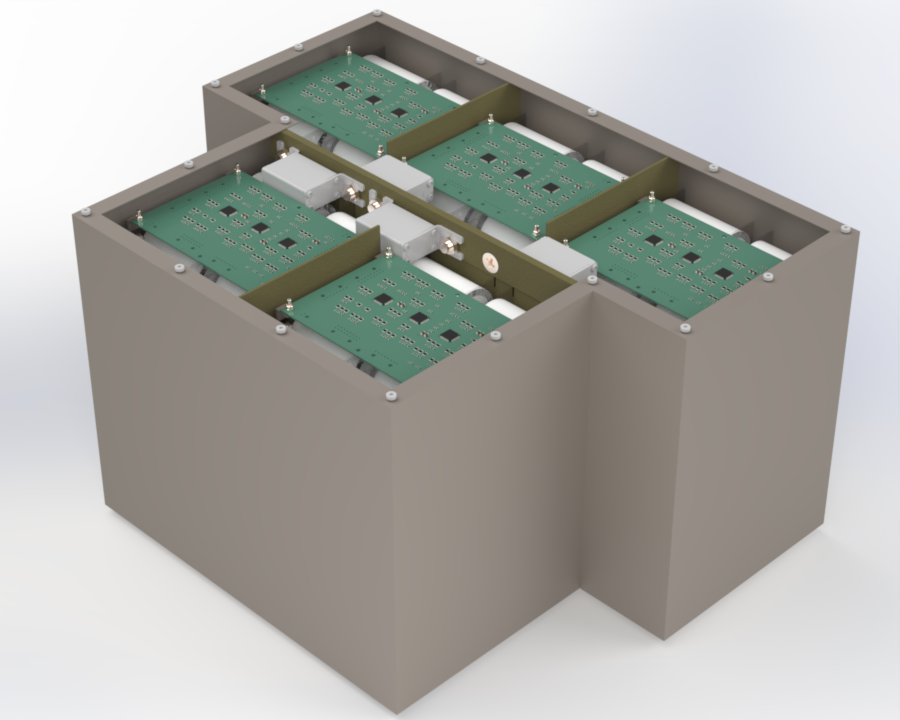
\includegraphics[width=1\textwidth]{figures/renders/main4.png}
    \caption{Accumulator design with lid removed for visibility.}
    \label{fig:main_accumulator}
\end{figure}

The accumulator is placed between driver and motor, below the inverter, to reduce HV cable mass and move mass near the rear axle. This packaging envelope drives the 3--2 segment arrangement. Vehicle-level packaging and the placement of the major powertrain components within the chassis are discussed in Section~\ref{sec:chassis_architecture} and illustrated in Figure~\ref{fig:components}.

The external casing is fabricated from stainless steel featuring 0.9 mm walls and a 1.2 mm floor to meet FS-EV~4.4.2 regulations. The three-piece assembly (removable bolted lid, welded lower shell, and base floor) enables service access while maintaining structural integrity.

Detailed manufacturing process planning, quality control workflow, and full bill of materials (BOM) costing are not expanded in this report and are deferred to implementation documentation.

\section{Results and Discussion}
\label{sec:results_discussion}

\subsection{Comparison with LiPo Baseline}

\begin{table}[htbp]
    \centering
    \caption{Comparison of EDLC supercapacitor, using results from design analysis, and high-power LiPo battery technologies, using motorsport-adapted simulation results \cite{batpac2022manual}. Weighted scoring system applied. Tie between the two technologies.}
    \label{tab:results_comparison}
    \footnotesize
    \begin{tabular}{|c|l|l|l|}
        \hline
        \textbf{Technology} & \makecell{\textbf{Mass} \\ \textbf{(kg)}} & \makecell{\textbf{Volume} \\ \textbf{(L)}} & \textbf{Evaluation Method} \\
        \hline
        EDLC Cap. & 36.0 & 44.5 & Design \\
        \arrayrulecolor{gray!30}\hline\arrayrulecolor{black}
        LiPo Battery & 40.3 & 30.3 & BatPac Sim \\
        \hline
        \hline
        \multicolumn{4}{|c|}{\textbf{Weighted Scoring Analysis}} \\
        \hline
        \textbf{Technology} & \textbf{Mass (3×)} & \textbf{Volume (1×)} & \textbf{Total Score} \\
        \hline
        EDLC & 3.00 & 0.68 & 3.68 \\
        \arrayrulecolor{gray!30}\hline\arrayrulecolor{black}
        LiPo & 2.68 & 1.00 & 3.68 \\
        \hline
        \textbf{Best} & \textbf{EDLC} & \textbf{LiPo} & \cellcolor{orange!20}\textbf{Tie} \\
        \hline
    \end{tabular}
\end{table}

Table~\ref{tab:results_comparison} evaluates the final design against the LiPo baseline using a more detailed model than Table~\ref{tab:tech_comparison}. SC mass and volume are taken from the CAD model, while LiPo results are adjusted to represent a complete pack. Cell volume is scaled by a cell-to-pack (CtP) ratio of 0.413 for pouch-cell FS designs \cite{epp_multiphysical_battery}. With a tie in weighted score, cost becomes the key differentiator once BOM costings are finalised; public pricing data for FS LiPo systems are limited, but they are generally reported to be significantly more expensive than the SC solution. Considering procurement risk and system complexity, the SC solution is preferred for this project context.

\subsection{Design Criteria Achievement}
\label{sec:design_criteria_achievement}
The finalised design is verified against the requirement IDs in Table~\ref{tab:design_requirement_ids}, using the LiPo comparison in Table~\ref{tab:results_comparison} as the supporting evidence for the minimisation targets:

\begin{table}[htbp]
    \centering
    \caption{Requirement verification matrix for final design outcomes.}
    \label{tab:design_verification_matrix}
    \footnotesize
    \setlength{\tabcolsep}{4pt}
    \renewcommand{\arraystretch}{0.95}
    \begin{tabular}{|c|p{5cm}|p{7.5cm}|p{2cm}|}
        \hline
        \textbf{ID} & \textbf{Target} & \textbf{Evidence} & \textbf{Status} \\
        \hline
        R1 & $80\,\text{kW}$ & 80 kW sustained across the event & Met \\
        R2 & $320\,\text{kJ}$ & 320 kJ available with manageable current & Met \\
        R3 & Minimise mass, volume, cost, and procurement risk & Table~\ref{tab:results_comparison} gives a tie on total score; qualitative factors favour SC solution & Partially evidenced \\
        \hline
    \end{tabular}
\end{table}

\section{Future Improvements and Conclusion}
\label{sec:future_improvements_conclusion}

\subsection{Refinements for Implementation}
The design establishes a coherent architecture suitable for prototyping and integration. Key refinement priorities for implementation include: (1) detailed thermal analysis; (2) AMS firmware development; (3) manufacturing partner engagement for cost and lead-time validation; and (4) comprehensive electrical \& mechanical testing.

\subsection{Future Improvements}

In the current simulation, the car is only ever traction- or power-limited, as shown by the vehicle dynamics simulation results in Section~\ref{sec:constraint_activity} and the final run trace in Figure~\ref{fig:final_run}. For the accumulator design, the major optimisation opportunity to improve performance is to reduce mass. The following approaches could be considered:
\begin{itemize}
    \item A lighter SC cell (SC2), albeit with increased voltage sag, due to lower capacity or higher ESR. This would require more accurate thermal management due to increased power losses.
    \item A hybrid/asymmetric SC cell, which would strike a balance between SCs and LiPo energy and power densities. However, limited commercial availability increases procurement risk and would require early supplier engagement and testing to validate performance claims.
\end{itemize}

\subsection{Conclusion}
The accumulator system design combines proven supercapacitor technology with modular electrical and mechanical architecture to meet Formula Student requirements for the acceleration application. The analysis demonstrates comparable quantitative performance to the LiPo baseline while reducing cost and procurement risk. Subsequent development should focus on prototype validation, thermal characterisation under representative operating conditions, and iterative refinement based on test data.

\pagebreak
\compactbib
% --- END INLINE: PaulVogelberg/Engineering/paul_body.tex ---
\end{refsection}

\begin{refsection}
% Body uses `figures/...` paths; prefix must be Engineering root (not .../figures/).
\graphicspath{{../HarryEmes/Engineering/}{../../figures/}}
% --- BEGIN INLINE: HarryEmes/Engineering/harry_body.tex ---
\chapterauthor{Vehicle Dynamics Simulation}{Harry Emes}
% =====================================================================

% ---------------------------------------------------------------------
\section{Introduction}
\label{sec:intro}
% ---------------------------------------------------------------------

This chapter builds an accurate, rules compliant simulation of the Formula Student acceleration event. It's goal is to simulate the performance of build and it is used to inform subsystem design choices before hardware is fixed.
The Formula Student Acceleration Event (FS-D~5) is a \SI{75}{\metre}
standing start and is subject to, FS-EV~2.2 which caps electrical power drawn from the
accumulator at \SI{80}{\kilo\watt}, and FS-D~5.3.1 disqualifies runs
over \SI{25}{\second}. A competitive configuration must be
traction-limited at launch and power-limited later while respecting
the power cap and avoiding front-axle lift (wheelieing). Mass, centre of gravity,
tyres, gearing, drivetrain efficiency, and electrical architecture are
all modelled by this system and the results as well as other real world factors external to performance are used to infom their ultimate design decisions.

This chapter presents simulation methodology
(Section~\ref{sec:methodology}); verification
(Section~\ref{sec:vv}); sensitivity and optimisation
(Section~\ref{sec:sensitivity}); and predicted performance for the
final configuration (Section~\ref{sec:final_run}).

% ---------------------------------------------------------------------
\section{Simulation Methodology}
\label{sec:methodology}
% ---------------------------------------------------------------------

The simulation solves a four-state longitudinal model
($\mathbf{x} = [x, v, \omega_{w,f}, \omega_{w,r}]^\top$) on a
\SI{1}{\milli\second} timestep, computing tyre, aerodynamic, rolling
and drive forces at each sub-step of a fourth-order Runge--Kutta
integrator. Weight is constant and acts at the centre of gravity; aerodynamic drag and
downforce scale with the square of velocity ; quasi-static load transfer causes normal forces on the axels; the Pacejka tyre model maps normal load and slip to
tractive force; and the powertrain supplies rear wheel torque subject to
the FS-EV~2.2 electrical power limit. Net longitudinal force advances the
state via RK4. Each following subsection specifies one component of this
balance.

% ---------------------------------------------------------------------
\subsection{Longitudinal equation of motion and effective mass}
\label{sec:eom}
% ---------------------------------------------------------------------

Newton's second law applied longitudinally to the vehicle centre of
mass gives

\begin{equation}
\left(m_v + \frac{4 I_w}{r_w^2}\right) a = F_x - F_\text{drag} - F_\text{rr},
\label{eq:eom}
\end{equation}

where $m_v$ is the vehicle mass including driver, $I_w$ is the
rotational inertia of a single road wheel about its spin axis, $r_w$
is the loaded wheel radius, $a$ is the longitudinal acceleration,
$F_x$ is the net tractive force at the contact patch, and
$F_\text{drag}$ and $F_\text{rr}$ are aerodynamic drag and rolling
resistance. The $4 I_w / r_w^2$ term is the translational mass
equivalent of the rotational inertia of four wheels. For the baseline
vehicle ($m_v = \SI{200}{\kilo\gram}$,
$I_w = \SI{0.10}{\kilo\gram\metre\squared}$,
$r_w = \SI{0.247}{\metre}$), this contributes
$4 I_w / r_w^2 = \SI{6.5}{\kilo\gram}$, a \SI{3.3}{\percent}
effective mass increase. It is small but non-negligible over a
\SI{75}{\metre} event and is included in the simulation.

% ---------------------------------------------------------------------
\subsection{Quasi-static longitudinal load transfer}
\label{sec:load_transfer}
% ---------------------------------------------------------------------

Under longitudinal acceleration, weight transfers from the front to
the rear axle. Taking moments about the rear contact patch gives the
static rear normal force

\begin{equation}
F_{z,r}^{\text{static}} = \frac{m_v g \, (L - L_{CG})}{L},
\qquad
F_{z,f}^{\text{static}} = m_v g - F_{z,r}^{\text{static}},
\label{eq:static_normal}
\end{equation}

where $L$ is the wheelbase and $L_{CG}$ is the longitudinal distance
from the front axle to the centre of gravity. The
acceleration-induced load transfer is

\begin{equation}
\Delta F_z = \frac{m_v \, a \, h_{CG}}{L},
\label{eq:load_transfer}
\end{equation}

with $h_{CG}$ the centre-of-gravity height above the ground. Combined
with aerodynamic downforce $F_{L,f}$, $F_{L,r}$, the instantaneous
axle normal forces are
\begin{equation}
\begin{aligned}
F_{z,f} &= F_{z,f}^\text{static} - (1 - k_\text{AS})\,\Delta F_z + F_{L,f},\\
F_{z,r} &= F_{z,r}^\text{static} + (1 - k_\text{AS})\,\Delta F_z + F_{L,r},\\
k_\text{AS} &= 0.2\,\text{AS}, \qquad 0 \le \text{AS} \le 1,
\end{aligned}
\label{eq:normal_forces}
\end{equation}
where $\text{AS}$ is the anti-squat dial referenced in Section~\ref{sec:antisquat_dynamic_toe}.

The wheelie onset occurs when $F_{z,f} \to 0$; in the absence of
downforce this gives
\begin{equation}
a_\text{wheelie} = \frac{F_{z,f}^\text{static} L}{(1 - k_\text{AS})\, m_v h_{CG}}
                 = \frac{g (L - L_{CG})}{(1 - k_\text{AS})\, h_{CG}}.
\label{eq:wheelie}
\end{equation}

For the baseline parameters ($L = \SI{1.60}{\metre}$,
$L_{CG} = \SI{1.14}{\metre}$, $h_{CG} = \SI{0.22}{\metre}$) and
$k_\text{AS}=0$ (equivalently $\text{AS}=0$), Eq.~\ref{eq:wheelie}
gives $a_\text{wheelie} = \SI{20.5}{\metre\per\second\squared}$,
comfortably above the simulated peak of
\SI{12.86}{\metre\per\second\squared}.

Anti-squat (Section~\ref{sec:antisquat_dynamic_toe})
enters Eq.~\ref{eq:normal_forces} and thereby Eq.~\ref{eq:wheelie}.
This allows us to keep more load on the front axle without dropping the centre of gravity or stretching the wheelbase.
In this two-axle longitudinal model, $\text{AS}$ and $k_\text{AS}$ are a reduced-order surrogate for how strongly the rear anti-squat geometry in Section~\ref{sec:antisquat_dynamic_toe} may redistribute axle loads around the rigid-body transfer. Given the approximate model for antisquat, we keep the effect numerically conservative.

% ---------------------------------------------------------------------
\subsection{Tyre force model}
\label{sec:tyre}
% ---------------------------------------------------------------------

The longitudinal tractive force at each driven axle follows

\begin{equation}
F_x = \mu(\kappa, F_z)\, F_z,
\qquad
\kappa = \frac{\omega_w r_w - v}{\max(|v|,\, v_\text{floor})},
\label{eq:slip_ratio}
\end{equation}

where $\kappa$ is the longitudinal slip ratio. The denominator is
floored at $v_\text{floor} = \SI{0.1}{\metre\per\second}$ to avoid
Eq.~\ref{eq:slip_ratio} having a divide by 0 error; below this velocity
the slip ratio has min/max of $\pm 1$, which is physically reasonable for a spinning wheel
against a stationary vehicle.

Longitudinal friction coefficient $\mu(\kappa, F_z)$ is evaluated with
the Pacejka Magic Formula \cite{pacejka2012},

\begin{equation}
\mu(\kappa, F_z) = D \sin\!\Big( C \arctan\!\big( B\kappa - E(B\kappa - \arctan(B\kappa)) \big) \Big),
\label{eq:pacejka}
\end{equation}

with load-dependent peak $D = F_z (p_{Dx1} + p_{Dx2}\,\Delta F_z /
F_{z,0})$ and dimensionless stiffness factor $B = p_{Kx1} +
p_{Kx2}\,\Delta F_z / F_{z,0}$.
The coefficients are listed in
Table~\ref{tab:pacejka}. They are derived from the Avon FSAE tyre
lateral data available to the group and typical FSAE longitudinal
characteristics reported in the literature \cite{milliken1995,
pacejka2012}, scaled to a representative slick peak friction coefficient
$\mu_\text{max} = 1.7$.

\begin{table}[H]
\centering
\caption{Pacejka Magic Formula coefficients used in the
configuration. Load sensitivity is captured through $p_{Dx2}$ and
$p_{Kx2}$; the reference load $F_{z,0}$ is chosen as a typical rear
axle load during acceleration.}
\label{tab:pacejka}
\footnotesize
\begin{tabular}{|l|c|l|}
\hline
\textbf{Coefficient} & \textbf{Value} & \textbf{Role} \\
\hline
Shape factor $C$                & 1.65   & Controls sharpness of the peak. \\
Peak-load coefficient $p_{Dx1}$ & 1.70   & Peak friction at nominal load. \\
Load-sensitivity $p_{Dx2}$      & $-0.12$ & Peak drops by 12\% per unit $\Delta F_z / F_{z,0}$. \\
Stiffness $p_{Kx1}$             & $35\,000$ N/rad & Sets curve slope at origin. \\
Stiffness load-sens. $p_{Kx2}$  & $-3\,000$ N/rad & Widens optimal slip at high load. \\
Curvature $E$                   & $0.10$ & Shape of the post-peak roll-off. \\
Reference load $F_{z,0}$        & \SI{1500}{\newton} & Normalisation; typical rear axle load. \\
\hline
\end{tabular}
\end{table}

\subsubsection{Thermal grip window}
\label{sec:thermal}

Tyre grip depends heavily on temperature. A thermal model overlays on the
Pacejka peak:

\begin{equation}
\mu_\text{peak}(T) = \mu_\text{peak,0}
\exp\!\left(-\frac{(T - T_\text{opt})^2}{2 \sigma^2}\right),
\label{eq:thermal}
\end{equation}

with $T_\text{opt} = \SI{80}{\celsius}$ and
$\sigma = \SI{60}{\kelvin}$ based on published FSAE slick data
\cite{milliken1995}. The model captures the essential effect that
cold tyres at launch ($T \sim \SI{25}{\celsius}$) operate at roughly
$0.87\,\mu_\text{peak,0}$, while well-warmed tyres
($T \sim T_\text{opt}$) deliver the full peak.

% ---------------------------------------------------------------------
\subsection{Powertrain and the electrical power limit}
\label{sec:powertrain}
% ---------------------------------------------------------------------

FS-EV~2.2 caps \textit{electrical} power at the accumulator outlet at
\SI{80}{\kilo\watt}. Limiting
motor torque alone is therefore insufficient as the same motor torque
corresponds to a range of electrical powers depending on motor speed,
drivetrain efficiency, and the time-varying DC-link voltage $V_{\mathrm{bus}}(t)$.

We model the chosen YASA P400R motor
($K_t = \SI{0.822}{\newton\metre\per\ampere}$, peak AC current
\SI{285}{\ampere} through the BAMOCAR PG-D3 inverter
\cite{bamocar_pg, yasa_p400r}), a gear ratio of
$N_g = 5.5$, a drivetrain efficiency of $\eta_\text{drv} = 0.95$, and
a \SI{600}{\volt} nominal supercapacitor bus (Section~\ref{subsec:supercapacitor_analysis}). For a
requested wheel torque $T_w^\text{req}$:

\begin{equation}
T_m = \frac{T_w^\text{req}}{N_g \, \eta_\text{drv}},
\qquad
I_m = \frac{T_m}{K_t},
\qquad
P_\text{elec} = V_{\mathrm{bus}}(t)\, I_m.
\label{eq:powertrain_basic}
\end{equation}
Here $P_{\mathrm{elec}}$ is the \emph{demanded} electrical power using torque-demand current $I_m$; the delivered current is $I_m^{\star}$ in Eq.~\ref{eq:power_limit}, so compliant electrical power satisfies $V_{\mathrm{bus}}(t)\,I_m^{\star}\le P_{\max}$.

The \SI{80}{\kilo\watt} cap is enforced by clipping motor current
first and mapping back to wheel torque:

\begin{equation}
I_m^\star = \min\!\left(I_m,\; \frac{P_\text{max}}{V_{\mathrm{bus}}(t)},\; I_\text{max}\right),
\qquad
T_w = K_t I_m^\star N_g \, \eta_\text{drv}.
\label{eq:power_limit}
\end{equation}
where $I_\text{max}$ is the inverter AC current ceiling (\SI{285}{\ampere} here).

The peak motor torque is $T_m^\text{peak} = K_t I_\text{max} =
\SI{234}{\newton\metre}$, so the constraint activates at motor speed
$\omega^\star = P_\text{max}/T_m^\text{peak} = \SI{341}{\radian\per\second}$
(\num{3260} rpm), corresponding to a vehicle speed of
$v^\star = \omega^\star r_w / N_g = \SI{15.4}{\metre\per\second}$
(\SI{55}{\kilo\metre\per\hour}).

% ---------------------------------------------------------------------
\subsection{Energy storage model and inverter-limited voltage window}
\label{sec:accum_storage_model}
% ---------------------------------------------------------------------

Pack sizing and constant-power discharge, including series resistance, are developed in Section~\ref{subsec:supercapacitor_analysis}:
\begin{gather}
E=\frac{1}{2}CV^2=\frac{1}{2}C(V_{\max}^2-V_{\min}^2)
\tag{\ref{eq:capacitor_energy}}\\
\frac{\mathrm{d}V}{\mathrm{d}t}
=-\frac{P}{C\,V}-\frac{P^2 R_{\mathrm{total}}}{C\,V^{3}}
\tag{\ref{eq:pack_voltage_dynamics}}
\end{gather}
where $R_{\mathrm{total}}=n\,\mathrm{ESR}_{\mathrm{cell}}$ for $n$ cells in series.
Equation~\eqref{eq:pack_voltage_dynamics} captures how the terminal voltage sags during discharge (Figure~\ref{fig:supercap_discharge}).
The discharge trace falls to about \SI{369}{\volt} at the end of the \SI{4}{\second}, and the powertrain assumes a minimum operating window of \SI{350}{\volt} for inverter/motor operation (Figure~\ref{fig:motor_operation}).
That leaves suitable margin at the bottom of the sag, so a falling DC link is acceptable: the inverter supplies torque by regulating motor current across the allowed voltage span, with $P_{\mathrm{elec}}\approx V_{\mathrm{bus}}(t)\,I_{\mathrm{dc}}$ implying higher DC-link current as $V_{\mathrm{bus}}(t)$ drops until FS-EV~2.2 or $I_\text{max}$ limits bind.

% ---------------------------------------------------------------------
\subsection{Launch strategy and traction control}
\label{sec:launch}
% ---------------------------------------------------------------------

The controller must avoid torque demands that cold
tyres and wheelie limits cannot support.
Figure~\ref{fig:launch_control_flow} shows how each commanded torque is
calculated each timestep before it is applied to the physical
model.

\begin{figure}[htbp]
\centering
\begin{singlespace}
\footnotesize
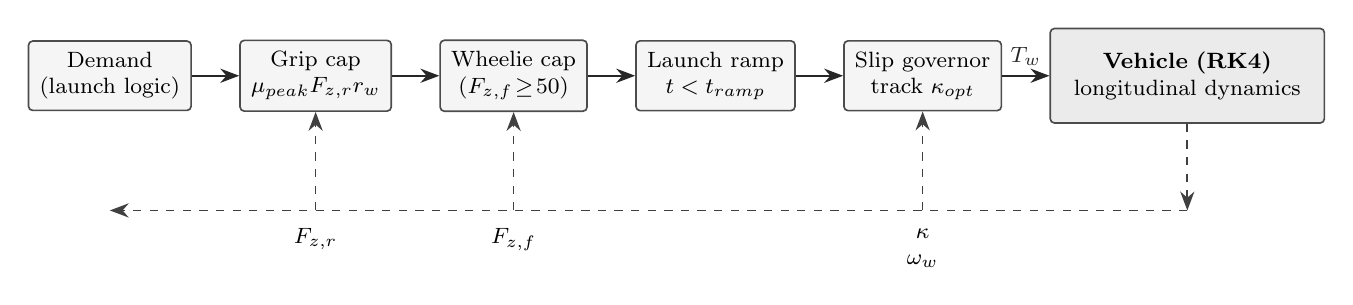
\begin{tikzpicture}[
  >={Stealth[length=2.4mm]},
  node distance=6mm and 6mm,
  blk/.style={rectangle, draw=black!70, line width=0.6pt, rounded corners=1.5pt,
              inner sep=4pt, align=center, font=\footnotesize, minimum height=8mm},
  ffblk/.style={blk, fill=black!4},
  plant/.style={blk, fill=black!8, minimum height=12mm, text width=32mm},
  sig/.style={font=\footnotesize\itshape},
  fb/.style={->, line width=0.6pt, black!75, dashed},
  ff/.style={->, line width=0.7pt, black!85}
]
% Feed-forward path
\node[ffblk] (dem)  {Demand\\(launch logic)};
\node[ffblk, right=of dem]    (grip)  {Grip cap\\$\mu_\text{peak} F_{z,r} r_w$};
\node[ffblk, right=of grip]   (whl)   {Wheelie cap\\($F_{z,f}\!\ge\!\SI{50}{\newton}$)};
\node[ffblk, right=of whl]    (ramp)  {Launch ramp\\$t<t_\text{ramp}$};
\node[ffblk, right=of ramp]   (slip)  {Slip governor\\track $\kappa_\text{opt}$};
\node[plant, right=of slip]   (plant) {\textbf{Vehicle (RK4)}\\longitudinal dynamics};

% Forward arrows
\draw[ff] (dem)  -- (grip);
\draw[ff] (grip) -- (whl);
\draw[ff] (whl)  -- (ramp);
\draw[ff] (ramp) -- (slip);
\draw[ff] (slip) -- node[above, sig] {$T_w$} (plant);

% Feedback bus: labels sit below the bus (clear of vertical taps)
\coordinate (busR) at ($(plant.south)+(0,-11mm)$);
\coordinate (busL) at (dem.south |- busR);
\draw[fb] (plant.south) -- (busR);
\draw[fb] (busR) -- (busL);

\path (grip.south |- busR) coordinate (bg);
\draw[fb] (bg) -- (grip.south);
\node[sig, below=3pt of bg, anchor=north] {$F_{z,r}$};

\path (whl.south |- busR) coordinate (bw);
\draw[fb] (bw) -- (whl.south);
\node[sig, below=3pt of bw, anchor=north] {$F_{z,f}$};

\path (slip.south |- busR) coordinate (bs);
\draw[fb] (bs) -- (slip.south);
\node[sig, below=3pt of bs, anchor=north, align=center] {$\kappa$\\$\omega_w$};
\end{tikzpicture}
\end{singlespace}
\caption{Launch traction-control block diagram. Solid arrows are feed-forward
torque conditioning (demand $\to$ grip cap $\to$ wheelie cap $\to$ \SI{65}{\milli\second}
S-curve ramp $\to$ slip governor); dashed arrows are feedback signals from the
RK4 system. Three feedback paths close the loop: rear normal load $F_{z,r}$ sets the
grip ceiling, front normal load $F_{z,f}$ scales the wheelie cap, and rear
slip $\kappa$ / wheel speed $\omega_w$ drive the slip-tracking governor.}
\label{fig:launch_control_flow}
\end{figure}

% ---------------------------------------------------------------------
\subsection{Aerodynamics}
\label{sec:aero}
% ---------------------------------------------------------------------

Aerodynamic drag and downforce are modelled with the standard
quadratic-velocity expressions

\begin{equation}
F_\text{drag} = \tfrac{1}{2} \rho \, C_d A \, v^2,
\qquad
F_{L,i} = \tfrac{1}{2} \rho \, C_{L,i} A_\text{ref} \, v^2
\quad (i = f, r).
\label{eq:aero}
\end{equation}

For the $C_d A = \SI{0.8}{\metre\squared}$ at sea-level
density $\rho = \SI{1.225}{\kilo\gram\per\metre\cubed}$, the drag
force at the terminal \SI{33}{\metre\per\second} is approximately
\SI{540}{\newton}, just \SI{8}{\percent} of the driving
force. Over the whole run, a $\pm 10\,\%$ perturbation of $C_{L,i} $
changes the \SI{75}{\metre} time by only $\pm\SI{8}{\milli\second}$
(Section~\ref{sec:tornado}), confirming that an aerodynamic package
with its associated mass and complexity has low marginal benefit for
this event and supports the group's decision to descope bodywork
development.

% ---------------------------------------------------------------------
\subsection{Numerical integration}
\label{sec:numerical}
% ---------------------------------------------------------------------

The state vector
$\mathbf{x} = [x, v, \omega_{w,f}, \omega_{w,r}]^\top$ evolves
according to four coupled ordinary differential equations. The Pacejka peak and the electrical clipping in
Eq.~\ref{eq:power_limit} can both influence the derivative within a
single timestep. The simulation therefore uses explicit fourth-order
Runge--Kutta integration \cite{press2007},

\begin{equation}
\mathbf{x}_{n+1} = \mathbf{x}_n + \frac{\Delta t}{6}\left(\mathbf{k}_1 + 2\mathbf{k}_2 + 2\mathbf{k}_3 + \mathbf{k}_4\right),
\label{eq:rk4}
\end{equation}

which has local truncation error $\mathcal{O}(\Delta t^5)$ and global
error $\mathcal{O}(\Delta t^4)$ at the cost of four force evaluations
per step. A timestep of $\Delta t = \SI{1}{\milli\second}$ is used
throughout; Section~\ref{sec:convergence} shows that this is
converged to within \SI{3}{\milli\second} of the limiting value
obtained at $\Delta t = \SI{0.2}{\milli\second}$.

% ---------------------------------------------------------------------
\subsection{Software architecture and tooling}
\label{sec:architecture}
% ---------------------------------------------------------------------

\begin{figure}[H]
\centering
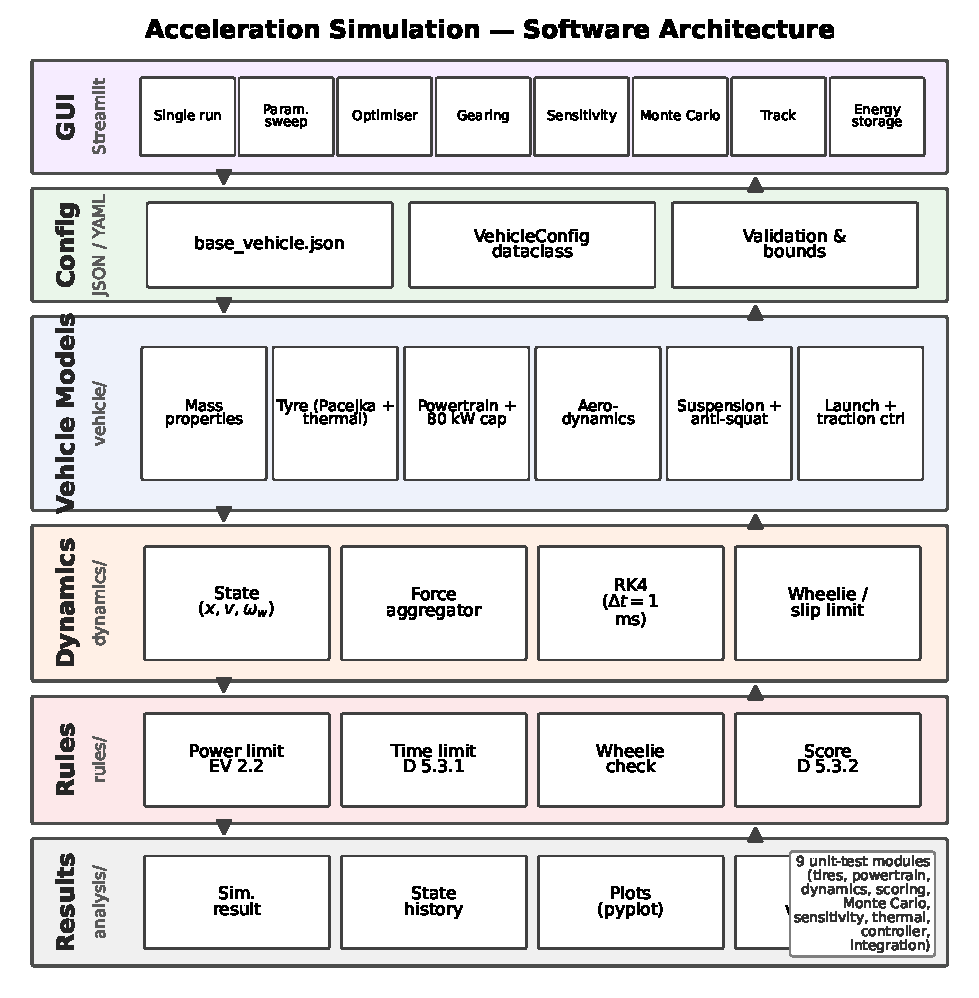
\includegraphics[width=0.95\textwidth]{figures/architecture.pdf}
\caption{Software architecture of the simulation. The five-layer
Python core (Config, Vehicle Models, Dynamics, Rules, Results)
enforces FS-EV~2.2 and FS-D~5.3.1 compliance on every simulated
configuration. A GUI sits above the core and is used
by the other subsystem chapters to evaluate parameter proposals
interactively.}
\label{fig:architecture}
\end{figure}

The simulation is organised as a five-layer Python simulation:
configuration, vehicle models, dynamics, rules, and results. All
vehicle parameters are externalised in JSON configuration files so
that any change proposed by another subsystem chapter can be
evaluated without modifying code. Rule compliance (FS-EV~2.2 and
FS-D~5.3.1) is enforced by a dedicated Rules layer that runs
automatically on each result, so no illegal configuration
can silently return a time.
For ease of use by the team, a GUI was developed for easy interface to the software.
The simulation also includes a series of other components
covering the tyre force model, powertrain and electrical limiting,
dynamics solver, scoring formula, Monte-Carlo robustness sampler,
sensitivity analyser, controller, and thermal overlay. Several others elements such as single-run, parameter sweep, optimiser, gearing study,
sensitivity, Monte Carlo and track conditions sits above the same
physics core and is used by the other subsystem chapters to evaluate
proposals (for example, the Drivetrain chapter's gear-ratio down-selection).

% ---------------------------------------------------------------------
\section{Verification and Validation}
\label{sec:vv}
% ---------------------------------------------------------------------

Three checks support the model: a constant-power lower bound
(Section~\ref{sec:analytical_bound}), algebraic spot checks
(Table~\ref{tab:handcalc}), and timestep convergence
(Section~\ref{sec:convergence}).

% ---------------------------------------------------------------------
\subsection{Analytical lower bound}
\label{sec:analytical_bound}
% ---------------------------------------------------------------------

If a car with mass $m$ was given constant power $P$ from rest with no drag,
rolling resistance, or traction limit, then
$v(t) = \sqrt{2Pt/m}$ and
$x(t) = \tfrac{2}{3}\sqrt{2P/m}\,t^{3/2}$. At $x=d=\SI{75}{\metre}$,

\begin{equation}
t_\text{cp} = \left(\frac{d}{\tfrac{2}{3}\sqrt{2P/m}}\right)^{2/3}.
\label{eq:analytical_bound}
\end{equation}

For $m=\SI{250}{\kilo\gram}$ and $P=\SI{80}{\kilo\watt}$,
Eq.~\ref{eq:analytical_bound} gives $t_\text{cp}=\SI{2.70}{\second}$
versus \SI{3.78}{\second} from the full simulator. The gap is dominated
by traction-limiting with drag and drivetrain losses being secondary factors. Rolling
resistance is negligible at this distance (Section~\ref{sec:tornado}).

% ---------------------------------------------------------------------
\subsection{Analytical hand-calculation agreement}
\label{sec:handcalc}
% ---------------------------------------------------------------------

Table~\ref{tab:handcalc} compares hand calculated estimates with the code for
rolling resistance and sustaining power at \SI{20}{\metre\per\second},
unramped launch acceleration at the torque cap, and the wheelie limit
from Eq.~\ref{eq:wheelie} evaluated at $k_\text{AS}=0$ for the hand column.

\begin{table}[H]
\centering
\caption{Algebraic checks vs.\ simulation (launch differs due to the
\SI{80}{\milli\second} ramp in Section~\ref{sec:launch}).}
\label{tab:handcalc}
\footnotesize
\setlength{\tabcolsep}{4pt}
\begin{tabularx}{\textwidth}{|>{\raggedright\arraybackslash\hsize=1.55\hsize}X|c|c|>{\raggedright\arraybackslash\hsize=0.45\hsize}X|}
\hline
\textbf{Quantity} & \textbf{Hand calc.} & \textbf{Simulation} & \textbf{Comment} \\
\hline
Rolling resistance at \SI{20}{\metre\per\second} (\si{\newton})
  & 24.5 & 24.5 & Exact; same $C_\text{rr}$. \\
Power to sustain \SI{20}{\metre\per\second} (\si{\watt})
  & 490 & 490 & Exact. \\
Launch accel., unramped cap (\si{\metre\per\second\squared})
  & 15.76 & 12.66 & Sim: \SI{80}{\milli\second} ramp. \\
Wheelie-limit accel.\ (\si{\metre\per\second\squared})
  & 20.51 & $\ge 12.86$ (no wheelie) & Margin \SI{37}{\percent}. \\
\hline
\end{tabularx}
\end{table}

% ---------------------------------------------------------------------
\subsection{Numerical convergence with timestep}
\label{sec:convergence}
% ---------------------------------------------------------------------

Table~\ref{tab:dt_convergence} lists $t_{75}$ for a coarse timestep, the
adopted $\Delta t=\SI{1}{\milli\second}$, and a reference at
\SI{0.2}{\milli\second}. At \SI{1}{\milli\second}, $t_{75}$ differs by
\SI{3}{\milli\second} (\SI{0.08}{\percent})---roughly
two orders of magnitude below the $\pm10\,\%$ single-parameter
sensitivities in Section~\ref{sec:tornado}, so discretisation error is
negligible next to modelling uncertainty.

\begin{table}[H]
\centering
\caption{$t_{75}$ vs.\ timestep (reference: $\Delta t=\SI{0.2}{\milli\second}$).}
\label{tab:dt_convergence}
\begingroup
\scriptsize
\setlength{\tabcolsep}{3pt}
\renewcommand{\arraystretch}{0.88}
\begin{tabular}{|c|c|c|}
\hline
$\Delta t$ (ms) & $t_{75}$ (s) & Deviation from ref.\ (ms) \\
\hline
5.00 & 3.825 & $+45.6$ \\
1.00 & 3.782 & $+2.6$ \\
0.20 & 3.779 & $0.0$ \\
\hline
\end{tabular}
\endgroup
\end{table}

% ---------------------------------------------------------------------
\section{Parameter Sensitivity and Design Optimisation}
\label{sec:sensitivity}
% ---------------------------------------------------------------------

The purpose of this section is to rank the vehicle
parameters by their influence on the \SI{75}{\metre} time
(Section~\ref{sec:tornado}), providing the target ranges used by the
other chapters. 

% ---------------------------------------------------------------------
\subsection{One-at-a-time sensitivity ranking}
\label{sec:tornado}
% ---------------------------------------------------------------------

\begin{figure}[H]
\centering

\includegraphics[width=0.68\textwidth]{figures/tornado.pdf}
\caption{One-at-a-time sensitivity of the \SI{75}{\metre} time to a
$\pm 10\,\%$ perturbation of each vehicle parameter. }
\label{fig:tornado}
\end{figure}

Figure~\ref{fig:tornado} summarises the sweep.
Each design parameter is perturbed by $\pm 10\,\%$ about the
baseline configuration, holding all others fixed, and the change in
predicted \SI{75}{\metre} time is recorded.
Dominant parameters are longitudinal CG and peak tyre grip, with wheel radius,
drivetrain efficiency, mass, and gear ratio forming a second tier.

The ranking has two practical consequences. First, the two dominant
parameters (longitudinal CG and tyre peak grip) sit in different subsystems
and have other constraints to consider: shifting the accumulator forward
to reduce $L_{CG}$ couples to mechanical packaging
(Section~\ref{sec:mechanical_design_packaging}), and raising peak grip is
constrained by tyre availability and budget within the suspension and
wheel package (Section~\ref{sec:suspension_requirements}). Second, the aerodynamic and
rolling-resistance contributions are sufficiently small that
investment in either is better deployed on mass or driveline
efficiency.

% ---------------------------------------------------------------------
\subsection{Monte Carlo robustness}
\label{sec:monte_carlo}
% ---------------------------------------------------------------------

A 500-sample Monte Carlo run was performed to quantify the
robustness of the predicted \SI{75}{\metre} time to realistically modeel the 
uncertainty in the parameters. Each sample draws total vehicle mass
($\sigma = \SI{8}{\kilo\gram}$), peak tyre grip
($p_{Dx1}$, $\sigma = 6\,\%$), longitudinal and vertical
centre-of-gravity positions
($\sigma = \SI{30}{\milli\metre}$ and \SI{15}{\milli\metre}),
drivetrain efficiency ($\sigma = 1.5\,\%$), and drag area
($\sigma = \SI{0.05}{\metre\squared}$) from independent Gaussians
around the baseline. The results are summarised in
Figure~\ref{fig:mc_histogram}.

\begin{figure}[H]
\centering
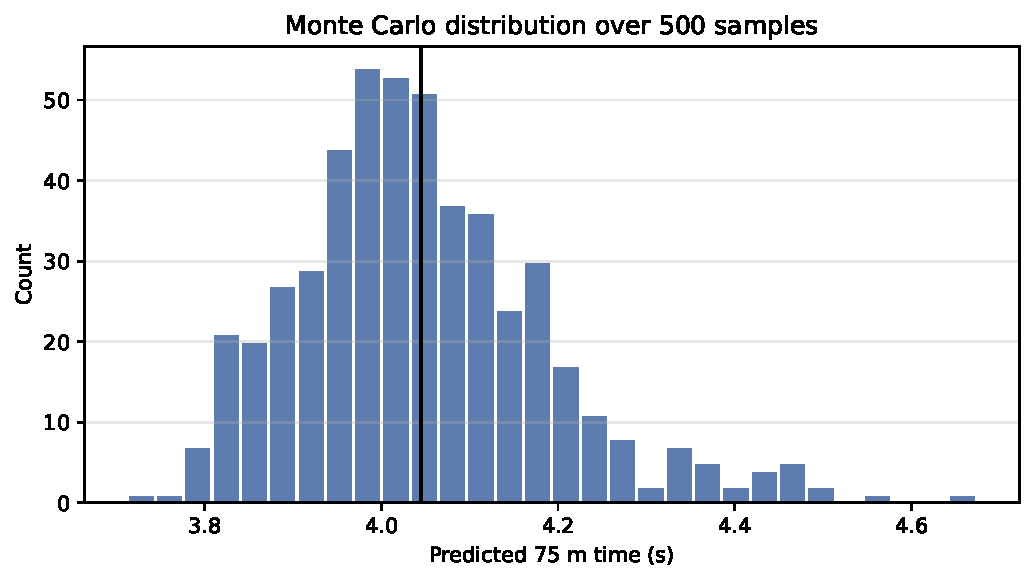
\includegraphics[width=0.82\textwidth]{figures/mc_histogram.pdf}
\caption{Distribution of predicted \SI{75}{\metre} time over
\num{500} Monte Carlo samples using the Gaussian parameter draws
described above.}
\label{fig:mc_histogram}
\end{figure}

Figure~\ref{fig:mc_histogram} summarises the sample distribution:
mean \SI{4.03}{\second} (standard deviation
\SI{120}{\milli\second}), with the 5--95 percentile band
\SIrange{3.86}{4.27}{\second}. The mean sits above the optimal
baseline \SI{3.78}{\second} and the histogram is positively skewed due to the 
unfavourable changes (lower grip, higher mass, higher CG) which cost more time.
in Section~\ref{sec:tornado}. Every sample remained compliant with
FS-EV~2.2 and FS-D~5.3.1 ($t_{75} < \SI{25}{\second}$) with no wheelie
($\min F_{z,f} > 0$), indicating substantial margin for the car.

% ---------------------------------------------------------------------
\subsection{Design optimisation}
\label{sec:optimisation}
% ---------------------------------------------------------------------

The sensitivity ranking above identifies which levers matter but does
not discuss their optimal combination. Several are coupled, such as gear
ratio and wheel radius through the driveline, CG position and
wheelbase through packaging, mass and grip through vertical load.
A formal optimisation is therefore performed over the seven
independent decision variables listed in
Table~\ref{tab:optim_setup}, with the remaining parameters held at
their hardware determined values (motor, inverter, supercapacitor pack,
FS rule limits).

\begin{table}[H]
\centering
\caption{Optimisation setup Seven decision variables with physically
motivated bounds. All other vehicle parameters are held at
hardware determined values corresponding to the YASA P400R motor, BAMOCAR
PG-D3 inverter, and \num{200}-cell supercap stack
\cite{bamocar_pg, yasa_p400r}.}
\label{tab:optim_setup}
\footnotesize
\begin{tabular}{|l|c|c|l|}
\hline
\textbf{Variable} & \textbf{Baseline} & \textbf{Bounds} & \textbf{Rationale} \\
\hline
Wheelbase $L$ (\si{\metre})               & 1.60 & [1.525, 1.75] & FS-T~2.9.1 min; packaging upper. \\
CG fraction $L_{CG}/L$                    & 0.71 & [0.50, 0.88] & RWD grip vs steering balance. \\
Gear ratio $N_g$                          & 5.5 & [3.0, 7.0] & Drivetrain chapter packaging. \\
Wheel radius $r_w$ (\si{\metre})          & 0.247 & [0.20, 0.28] & 10-inch vs 13-inch rim options. \\
Pacejka $\kappa_\text{opt}$               & 0.14 & [0.08, 0.20] & Slick tyre literature range. \\
Launch torque limit (\si{\newton\metre})  & 1000 & [400, 1200] & YASA peak torque. \\
Anti-squat $\text{AS}$                    & 0.12 & [0.00, 1.00] & Section~\ref{sec:antisquat_dynamic_toe}. \\
\hline
\end{tabular}
\end{table}

The objective is to minimise the \SI{75}{\metre} time subject to three
constraints enforced by the Rules layer: FS-EV~2.2 (peak electrical
power $\leq \SI{80}{\kilo\watt}$), FS-D~5.3.1 (finish time
$< \SI{25}{\second}$), and no wheelie
($\min F_{z,f} > 0$). Configurations that violate them return their full time but are
reported as non-compliant.
SciPy's Nelder--Mead optimiser \cite{press2007} minimises \(t_{75}\) by
trying new parameter sets and comparing simulated times in order to tune seven parameters.

Over \num{243} objective evaluations the best feasible time decreased
monotonically from the \SI{3.78}{\second} baseline to
\textbf{\SI{3.67}{\second}}, a \SI{2.9}{\percent} improvement
(Table~\ref{tab:optim_result}). Wheelie-violating candidates were
rejected via the objective penalty; at the optimum all three
constraints (FS-EV~2.2, FS-D~5.3.1, $\min F_{z,f} > 0$) are
satisfied with comfortable margin on front normal force.

\begin{table}[H]
\centering
\caption{Optimisation results and changes to parameters.}
\label{tab:optim_result}
\footnotesize
\begin{tabular}{|l|c|c|c|}
\hline
\textbf{Variable} & \textbf{Baseline} & \textbf{Optimised} & \textbf{Change} \\
\hline
Wheelbase $L$ (\si{\metre})      & 1.60 & 1.60 & -- \\
CG fraction $L_{CG}/L$           & 0.71 & 0.63 & $-11\,\%$ \\
Gear ratio $N_g$                 & 5.5 & 4.94 & $-10\,\%$ \\
Wheel radius $r_w$ (\si{\metre}) & 0.247 & 0.227 & $-8\,\%$ \\
Pacejka $\kappa_\text{opt}$      & 0.140 & 0.132 & $-6\,\%$ \\
Launch torque (\si{\newton\metre}) & 1000 & 721 & $-28\,\%$ \\
Anti-squat $\text{AS}$            & 0.12 & 0.36 & $+200\,\%$ \\
\hline
\textbf{\SI{75}{\metre} time (\si{\second})} & \textbf{3.78} & \textbf{3.67} & $\mathbf{-2.9\,\%}$ \\
\hline
\end{tabular}
\end{table}

The optimiser's choices have physical interpretations. The CG shift
forward and the anti-squat increase together preserve front normal
force despite the reduced launch torque cap ; the smaller
wheel and tighter gear ratio increase tractive force at the cost of
top speed, but the extra top-speed margin is not needed over
\SI{75}{\metre}. These results feed back to the neighbouring
chapters as the vehicle-level targets summarised in
Section~\ref{sec:final_params}.

% ---------------------------------------------------------------------
\subsection{Robustness to track surface conditions}
\label{sec:drywet}
% ---------------------------------------------------------------------

The ambient conditions for the track may vary on the day. 
Scaling the Pacejka peak grip by a
surface condition multiplier (\num{1.0} for dry slicks on clean
tarmac, \num{0.60} for the same slicks on a water film
\cite{milliken1995}) gives a wet-track prediction of
\SI{4.83}{\second} versus \SI{3.78}{\second} dry --- a
\SI{28}{\percent} time penalty (Figure~\ref{fig:drywet}). In wet conditions the phase transition
(Section~\ref{sec:constraint_activity}) shifts later in the run: the
vehicle spends more of the event traction-limited and less of it
power-limited, which is consistent with the intuitive result.

\begin{figure}[H]
\centering
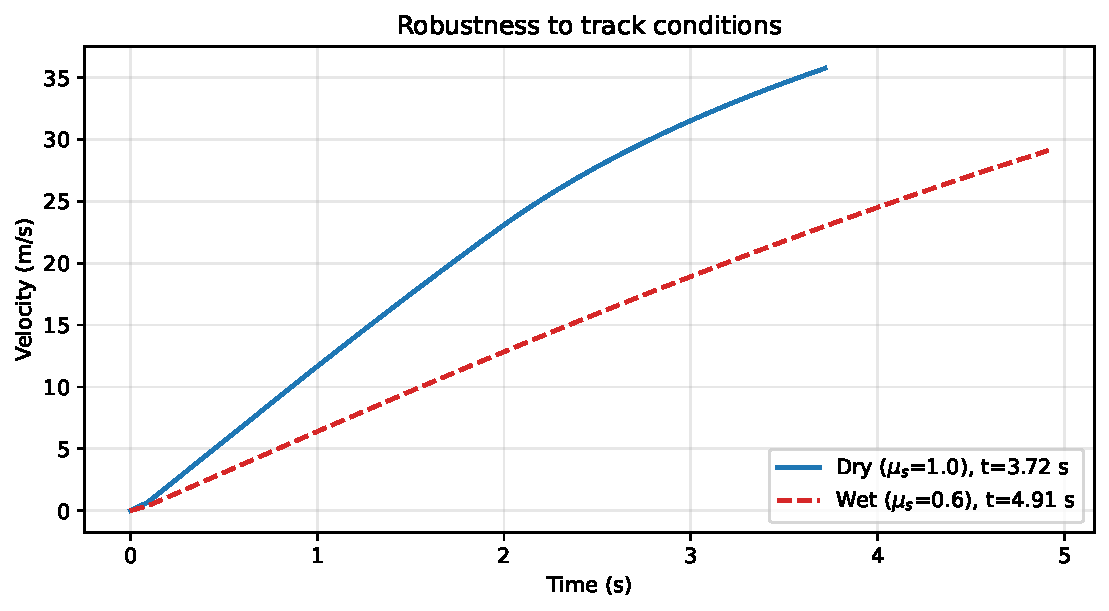
\includegraphics[width=0.68\textwidth,height=0.42\textheight,keepaspectratio]{figures/dry_wet.pdf}
\caption{Velocity trace under dry and wet surface conditions (peak
grip multiplier \num{1.0} vs \num{0.60}).}
\label{fig:drywet}
\end{figure}

% ---------------------------------------------------------------------
\section{Predicted Performance of the Final Vehicle}
\label{sec:final_run}
% ---------------------------------------------------------------------

The final agreed vehicle configuration combines decisions across the
Chassis, Suspension, Drivetrain, and Supercapacitors chapters. The
simulation takes the finalised configuration as input and produces
predicted performance traces.

% ---------------------------------------------------------------------
\subsection{Final agreed parameter set}
\label{sec:final_params}
% ---------------------------------------------------------------------

\begin{table}[H]
\centering
\caption{Final agreed parameter set: principal inputs matching the
longitudinal simulation baseline (Section~\ref{sec:monte_carlo},
Table~\ref{tab:pacejka}), with electrical hardware figures from the
Drivetrain and Supercapacitors chapters.}
\label{tab:final_parameters}
\footnotesize
\begin{tabular}{|l|c|c|l|}
\hline
\textbf{Parameter} & \textbf{Symbol} & \textbf{Value} & \textbf{Source} \\
\hline
Total vehicle mass & $m_v$ & 200\si{\kilo\gram} & Section~\ref{sec:monte_carlo}; chassis $<$\SI{220}{\kilo\gram} \\
Wheelbase & $L$ & 1.60\si{\metre} & Chassis \\
CG longitudinal & $L_{CG}$ & 1.14\si{\metre} & Section~\ref{sec:load_transfer} \\
CG height & $h_{CG}$ & 0.22\si{\metre} & Section~\ref{sec:load_transfer} \\
Wheel radius & $r_w$ & 0.247\si{\metre} & Section~\ref{sec:monte_carlo}; loaded radius \\
Peak tyre grip & $p_{Dx1}$ & 1.70 & Table~\ref{tab:pacejka} \\
Accumulator nominal voltage & $V_{\mathrm{bus}}(t)$ & \SI{600}{\volt} (nominal) & Section~\ref{sec:accum_storage_model} \\
Accumulator mass & $m_\text{acc}$ & 27.8\si{\kilo\gram} & Supercapacitors \\
Motor torque constant & $K_t$ & 0.822\si{\newton\metre\per\ampere} & Drivetrain (YASA P400R) \\
Motor peak RMS current & $I_m^\text{peak}$ & 285\si{\ampere} & Drivetrain (BAMOCAR PG-D3) \\
Gear ratio & $N_g$ & 5.5 & Section~\ref{sec:powertrain} \\
Drivetrain efficiency & $\eta_\text{drv}$ & 0.95 & Section~\ref{sec:powertrain} \\
Drag area & $C_d A$ & 0.80\si{\metre\squared} & Chassis \\
Anti-squat ratio & $\text{AS}$ & 0.36 & Section~\ref{sec:monte_carlo}; geometry Section~\ref{sec:antisquat_dynamic_toe} \\
\hline
\end{tabular}
\medskip

\noindent\footnotesize\textit{Note.}
The runnable simulation configuration contains many further parameters
(for example full tyre coefficients, launch-controller timings, and
numerical settings); Table~\ref{tab:final_parameters} lists only the
main quantities needed for cross-chapter integration.
\end{table}

% ---------------------------------------------------------------------
\subsection{Constraint activity and phase analysis}
\label{sec:constraint_activity}
% ---------------------------------------------------------------------

Figure~\ref{fig:final_run} shows the predicted four-channel trace of
the baseline vehicle, anchoring the numerical discussion while the
final agreed parameters are confirmed. Three features are worth
commenting on explicitly, because they determine where design effort
is most profitably spent.

\begin{figure}[H]
\centering
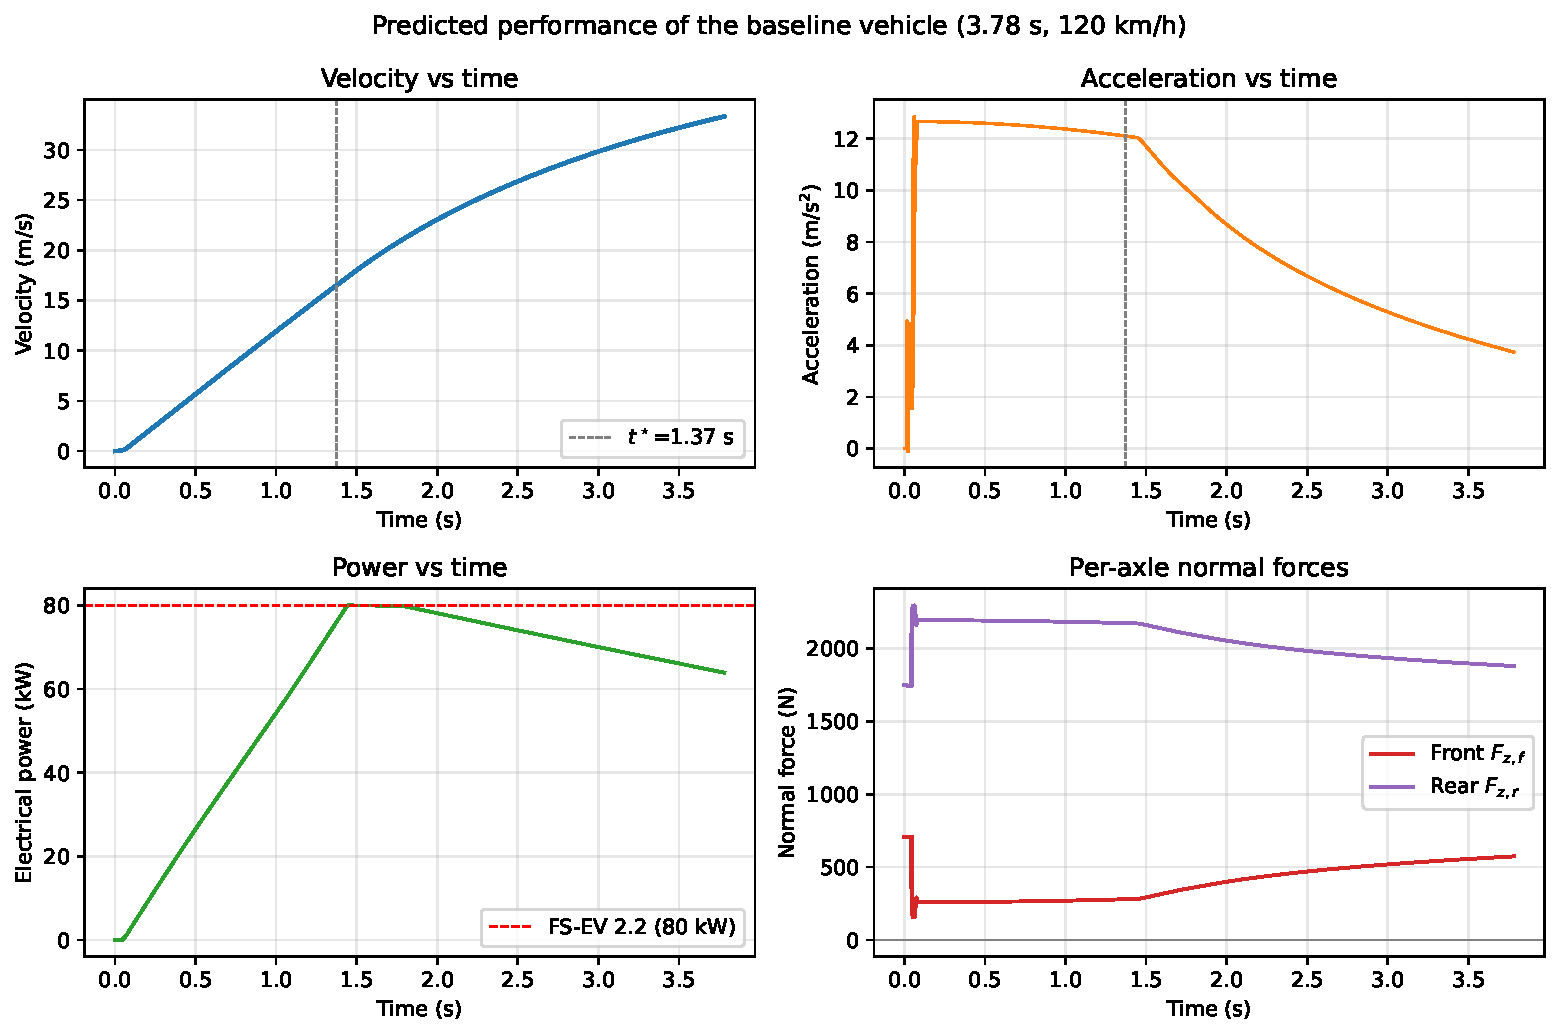
\includegraphics[width=0.95\textwidth]{figures/final_run.pdf}
\caption{Predicted performance of the baseline vehicle. The
grey dashed line at $t^\star = \SI{1.37}{\second}$ marks the
transition from the traction-limited to the power-limited regime.
Instantaneous electrical power (lower left) saturates cleanly at
the FS-EV~2.2 cap, and the front normal force (lower right) remains
positive throughout the run.}
\label{fig:final_run}
\end{figure}

First, the vehicle spends \SI{1.37}{\second} (\SI{36}{\percent} of
the total run time) in the traction-limited regime and
\SI{2.41}{\second} (\SI{64}{\percent}) in the power-limited regime,
with the transition occurring at
$v^\star = \SI{15.4}{\metre\per\second}$ as predicted analytically
in Section~\ref{sec:powertrain}. The grip utilisation during the
traction-limited phase averages approximately \SI{103}{\percent}
relative to the reference Pacejka peak, confirming the launch
controller (Section~\ref{sec:launch}) tracks the load-dependent grip
ceiling closely.

Second, the electrical power saturates cleanly at \SI{79.80}{\kilo\watt}
(against the \SI{80}{\kilo\watt} cap), without overshoot, throughout
the power-limited phase. This is the evidence that
Eq.~\ref{eq:power_limit} is correctly enforced at the electrical
side rather than at the wheel.

Third, the front normal force falls smoothly from a static
\SI{707}{\newton} to a minimum of \SI{158}{\newton} at peak
acceleration and recovers as the vehicle enters the power-limited
phase. The \SI{158}{\newton} minimum is a \SI{22}{\percent} fraction
of the static load, which is ample margin against the wheelie
threshold and validates the choice of anti-squat and CG
geometry for the baseline configuration.

% ---------------------------------------------------------------------
\section{Discussion and Limitations}
\label{sec:discussion}
% ---------------------------------------------------------------------

The simulation is highly detailed and
consistent with the validation evidence in Section~\ref{sec:vv}, but it
omits a few other models that could reduce the gap between sim and reality. Main gaps:
\textbf{driveline torsional compliance} (minor launch oscillation; beyond the rigid torque path implied by Section~\ref{sec:mechanical_design_packaging}),
\textbf{motor electrical dynamics} (finite torque rise time and brief dips; beyond the quasi-static electrical limit in Section~\ref{sec:powertrain}),
\textbf{electrical dynamics beyond quasi-static $V_{\mathrm{bus}}(t)$:} inverter/motor current-control transients and line effects not resolved in Sections~\ref{sec:powertrain}--\ref{sec:accum_storage_model}, and \textbf{driver reaction time}
(\SIrange{0.2}{0.4}{\second} omitted). Combined with
Section~\ref{sec:monte_carlo}, the headline \SI{75}{\metre} time is
estimated within roughly $\pm \SI{0.20}{\second}$. Adding a typical
\SIrange{0.2}{0.4}{\second} driver reaction delay to the Monte Carlo
mean of \SI{4.03}{\second} (Section~\ref{sec:monte_carlo}) gives a
realistic on-event prediction of
\SIrange{4.23}{4.43}{\second}, which sits comfortably within the band
of published Formula Student Electric times at FSG~2023
\cite{fsg_results_2023}, confirming that the deterministic
\SI{3.78}{\second} baseline is best read as a knife-edge optimum
rather than an expected race-day figure.

% ---------------------------------------------------------------------
\section{Conclusions and Further Work}
\label{sec:conclusions}
% ---------------------------------------------------------------------

\noindent 
This chapter built an accurate simulation with FS electrical and timing rules enforced at each timestep. The conclusions below discuss the validated predictions, dominant sensitivities, optimisation result, uncertainty band, and scoring readout that follow from that model.
Section~\ref{sec:vv} gives hand checks, timestep convergence, and a constant-power bound; Section~\ref{sec:tornado} ranks longitudinal centre of gravity and peak grip as the dominant levers on the \SI{75}{\metre} time, with wheel radius, driveline efficiency, mass, and gear ratio as a secondary band.
Nelder--Mead over \num{243} evaluations reaches \SI{3.67}{\second} from a \SI{3.78}{\second} baseline under FS-EV~2.2, FS-D~5.3.1, and with non-wheelie conditions (Section~\ref{sec:optimisation}); wet grip scaling preserves the same compliance (Section~\ref{sec:drywet}).
The \num{500}-draw Monte Carlo mean is \SI{4.03}{\second} with 5--95 band \SIrange{3.86}{4.27}{\second} and full sample compliance (Section~\ref{sec:monte_carlo}); the baseline trace matches the predicted traction-to-power split and~$v^\star$ (Section~\ref{sec:constraint_activity}).
Adding a typical \SIrange{0.2}{0.4}{\second} driver reaction delay to that mean implies an on-event band of about \SIrange{4.23}{4.43}{\second}, which is consistent with published Formula Student Electric acceleration times at FSG~2023~\cite{fsg_results_2023}.
Under FS-D~5.3.2 with notional $T_\text{fastest}=\SI{3.5}{\second}$, the baseline and optimised sets map to \num{59.2}/75 and \num{65.1}/75 points respectively.

\subsection{Further work}
\label{sec:further_work}

Future development should focus on improving the physical fidelity of the model and decreasing the gap to real-world vehicle behaviour.
The highest-priority improvement is calibration of the Pacejka tyre coefficients using empirical tyre testing data, since tyre grip was identified as the dominant sensitivity parameter in the acceleration event (Section~\ref{sec:tornado}).

Further work should also include:
\begin{itemize}
    \item modelling driveline torsional compliance to capture launch oscillations and wheel-hop behaviour;
    \item inclusion of motor electrical transient dynamics and finite torque rise time;
    \item integration of suspension compliance and chassis flexibility effects;
    \item experimental validation against telemetry from a physical prototype;
    \item extension of the model to include thermal degradation during repeated launch cycles.
\end{itemize}

Additional random modelling of track contamination, tyre temperature evolution, and driver reaction variability would also improve robustness predictions for real competition conditions.

% ---------------------------------------------------------------------
\compactbib
% ---------------------------------------------------------------------

% --- END INLINE: HarryEmes/Engineering/harry_body.tex ---
\end{refsection}

% --------------------------------------------------------------------
% Business chapters: Toby, Paul, Ziyang Xing, Yuze, Harry
% --------------------------------------------------------------------

\begin{refsection}
\graphicspath{{../TobyMcConnell/Business/}}
% --- BEGIN INLINE: TobyMcConnell/Business/toby_business_body.tex ---
\chapterauthor{Market and Competition Analysis}{Toby McConnell}
\label{sec:market_and_competition}

\section{Introduction and Executive Summary}

Chapters 1 to 4 established the vehicle’s structural base and design elements (chassis, suspension, powertrain, and accumulator design), while Chapter 5 integrated these systems through simulation to validate its 3.73-second sprint capability. Chapters 6 onwards pivots from technical engineering to commercial strategy.

This commercial strategy introduces a Testing-as-a-Service (TaaS) model centered on an adapted version of the FS car, transitioning it from a sprint vehicle into a high-performance physical testing platform developed for advanced brake testing and autonomous vehicle (AV) validation in a business-to-business (B2B) context.

This Chapter 6 introduces our core value proposition and applies a market segmentation framework to justify a strategic focus on the autonomous sector in the Uk, identifying high-priority entry points and target customers through competitive landscape evaluation, personas, and user journey mapping. Chapter \ref{chap:strategy_stakeholder_analysis} continues with stakeholder adoption and go-to-market execution.

\section{Product Overview and Value Proposition}
\label{sec:value}

The operational foundation of this service is a modified high-dynamic vehicle that functions as a moving target for AV systems, recreating complex real-world scenarios where rapid braking, turning, or emergency decision-making is required. To transform the base FS design into a regulated testing platform, the architecture will be updated with sophisticated data-logging features and interchangeable body shells for varied test environments.

A central element of this proposal is the inheritance of the vehicle's original design constraints. Having been designed to meet strict Formula Student regulations—including a cockpit sized for a 95th percentile male—the vehicle possesses features that are strictly redundant for an unmanned (AV) testing platform. While these constraints present a potential competitive disadvantage, they are a fundamental reality of the base car’s origin. Consequently, following supervisor guidance, this business proposal proceeds with the assumption that the base product utilises the existing high-performance supercapacitor accumulator, powertrain, and wheel design, while acknowledging that inherited constraints of the FS regulatory framework are treated as fixed design parameters, Section \ref{sec:sprint} shows how these same characteristics could define the commercial opportunity rather than limit it.

Our service-based model allows clients to access advanced testing capabilities without the capital expenditure or maintenance burdens of in-house facilities. This value proposition is structured around three primary benefits:

\begin{itemize}
\item \textbf{Data Quality} -- The service enables consistent braking tests due to the supercapacitor power supply and can operate under extreme conditions enabled by tyre and chassis design. This improves validation accuracy and reduces uncertainty in performance evaluation.

\item \textbf{Scenario Flexibility} -- Modular configuration with different shells allowing clients to simulate different braking conditions and edge cases without the overhead of large-scale facility changes.

\item \textbf{Testing Realism} -- Physical testing reduces reliance on software-only validation and helps close the simulation-to-reality gap in autonomous systems development. These tests provide a more accurate representation of real-world decision-making, braking, and crash scenarios, which simulations cannot fully replicate. This makes the service particularly valuable for final-stage vehicle validation.

\item \textbf{Client Affordability} -- Clients access advanced testing capabilities without the capital expenditure or maintenance burdens of in-house facilities, lowering the cost barrier to high-quality AV validation. How these benefits are delivered as a paid testing service is developed in Chapter \ref{chap:strategy_stakeholder_analysis}.
\end{itemize}

Together, these four benefits define the platform's position in the AV validation market. It acts as a “pain reliever” for slow, expensive testing cycles and a “gain creator” for safety validation confidence. The market segmentation and customer targeting that follows is built around this value proposition.

\section{Market Segmentation Strategy Overview}
\label{sec:segmentation}

Market segmentation is essential for identifying groups of customers who seek similar benefits and features from a product. Rather than treating the market as homogeneous, segmentation enables us to tailor value propositions and targeting strategies to distinct user needs.

In this project, demographic segmentation is not appropriate due to the business-to-business nature of the proposed testing platform targeting at organisations rather than individuals, meaning factors such as age or gender provide limited strategic insight. Instead, a hybrid segmentation approach is adopted, combining user-based segmentation with benefits-based segmentation and occasion-based segmentation. This allows identification of both the types of organisations using the product and the specific outcomes they seek. 

\begin{itemize}
    \item \textbf{User-based segmentation:} Categorizes customers by their role within the automotive ecosystem. This includes regulatory agencies, Original Equipment Manufacturers (OEMs), EV startups, and autonomous technology firms. For example, regulatory bodies prioritize certification reliability, whereas AV developers require rapid iteration and flexibility.
    
    \item \textbf{Benefits-based segmentation:} This focuses on the value delivered by the platform. Key benefits include high-speed repeatability, real-world testing conditions, adaptability of test scenarios, and cost efficiency relative to large proving grounds. These benefits do not hold equal importance across all user groups, helping identify customers most aligned with the product’s capabilities.
    
    \item \textbf{Occasion-based segmentation:} Testing needs vary depending on context, such as regulatory certification, early-stage research and development, or edge-case AI validation. Each occasion places different emphasis on flexibility, repeatability, and testing speed.
\end{itemize}

This hybrid framework ensures that segments are defined by both the type of target organisation and the outcomes they value, forming the basis for the following market analysis and comparisons.

\section{Market Option 1: Government Brake Testing Market}

\subsection{Market Overview and Size Estimation} 

The government brake testing market includes organisations responsible for validating vehicle braking performance against safety standards. This market spans multiple stages, each relying on established methods designed to prioritise repeatability and regulatory acceptance:

\begin{itemize}
    \item \textbf{Manufacturer pre-certification testing:} Automotive manufacturers typically conduct in--house braking validation before certification using track--based testing, dynamometers, and simulation tools such as finite element modelling (FEM) with, e.g., Ansys and MSC Software.
    
    \item \textbf{Government-regulated certification testing:} Certification bodies, like the Driver and Vehicle Standards Agency (DVSA) in the UK, use standardised equipment such as roller brake testers and calibrated decelerometers to measure braking performance with equipment suppliers such as MAHA Maschinenbau Haldenwang providing certified systems
    
    \item \textbf{Periodic roadworthiness inspection (e.g. MOT testing):} These tests typically use compact roller brake testers or portable decelerometers not track-based testing. Suppliers such as Tecalemit Garage Equipment and Capelec provide brake testing hardware commonly used in inspection centres. 
\end{itemize}

To estimate the size of this market we use a top-down estimation approach. The global brake tester market is estimated at $\sim$ 1.5 billion USD {\cite{promarketreports_brake_tester}}. As the majority of brake testing equipment is used in manufacturer validation, certification testing, and periodic inspection, this segment is estimated to account for approximatly 40\% of the total brake testing market. Therefore:
\begin{equation}
\begin{aligned}
\text{Gov. Brake Testing Market} &= 1.5 \times 0.40 \\
&= 0.60 \text{ billion USD}
\end{aligned}
\end{equation}
\vspace{+6pt}
This yields an estimated addressable market of approximately \$600 million globally.
\vspace{-10pt}
\subsection{Market Segmentation}

User-based segmentation identifies regulatory agencies, certification laboratories, and inspection operators as primary customers operating within strict compliance frameworks. Benefits-based segmentation shows a strong focus on reliability, standardisation, and regulatory acceptance, with limited emphasis on flexibility. Occasion-based segmentation highlights that testing occurs primarily during certification and compliance checks, requiring fixed procedures
Together, these segmentation perspectives indicate limited alignment between the market’s priorities and the platform’s core value proposition.

\subsection{Commercial Challenges}
\label{sec:commercial_challenges}

This market also presents significant commercial challenges. Entry barriers are high due to certification requirements and the need to demonstrate equivalence with established methods, while procurement cycles are long and complex.
Product-market fit is also limited. Customers prioritise consistency and risk minimisation, whereas the platform’s core advantages lie in flexibility and adaptability.
Scalability is constrained by a small customer base and varying international regulations, increasing the need for customisation and slowing expansion.

Overall, despite functional relevance, high barriers, weak alignment, and limited scalability make this market unattractive for an early-stage product and rule it out as a viable market entry point.

\section{Market Option 2: AI and Autonomous Vehicle Testing Market}

\subsection{Market Overview and Size Estimation}

The AI and autonomous vehicle testing market consists of automotive manufacturers, electric vehicle startups, and technology firms developing automated driving systems that require validation in complex real-world scenarios. As investment in automated driving has increased, organisations have placed greater emphasis on testing environments capable of validating decision-making, perception systems, and emergency braking behaviour.

The autonomous vehicle testing market can be estimated using a top-down approach. The global autonomous vehicle market is valued at $\sim$\$68.09 billion USD {\cite{grandview_autonomous_market}}. Automotive manufacturers typically allocate approximately 5--10\% of revenue to research and development, with higher values observed in innovation-intensive areas such as autonomous driving. A value of 10\% is therefore assumed:
\vspace{-9pt}
\begin{equation}
\begin{aligned}
\text{R\&D Budget} &= 68.09 \times 0.10 \\
&= 6.81 \text{ billion USD}
\end{aligned}
\end{equation}
\vspace{-2pt}

Testing and validation activities often account for $\sim$20--30\% {\cite{mckinsey_testing_validation}} of development effort in safety-critical automotive systems. Using a value of 25\%, the addressable testing market can be estimated.

\vspace{-15pt}
\begin{equation}
\begin{aligned}
\text{Testing Market} &= 6.81 \times 0.25 \\
&= 1.70 \text{ billion USD}
\end{aligned}
\end{equation}
\vspace{-5pt}

Therefore, the autonomous vehicle testing market is estimated at approximately \$1.5--2 billion globally and is projected to grow at a compound annual growth rate of 19.9\% {\cite{grandview_autonomous_market}} from 2025 to 2030. 

%\begin{table}[h]
%\centering
%\caption{Market Size Comparison}
%\begin{tabular}{|l|c|c|c|}
%\hline
%\textbf{Market} & \textbf{Estimated Size} & \textbf{Growth Rate} & \textbf{Attractiveness} \\
%\hline
%Government Brake Testing & \$0.5--0.7B & Low & Limited scalability \\
%\hline
%AI \& Autonomous Testing & \$1.5--2B & High & Strong growth potential \\
%\hline
%end{tabular}
%\label{tab:market_comparison}
%\end{table}

\subsection{Market Segmentation}

User-based segmentation identifies autonomous vehicle R\&D teams, EV startups, AV developers and automotive innovation divisions as primary customers. These organisations are actively developing automated driving systems and require frequent testing during development. Compared with regulatory bodies, they typically have faster decision-making processes and a greater willingness to adopt new testing technologies.
Benefits-based segmentation highlights that customers prioritise flexibility, rapid iteration, and real-world validation. Autonomous systems must be tested across a wide range of edge cases, including emergency braking scenarios. These requirements align closely with a platform capable of repeatable high-speed testing and configurable conditions.
Occasion-based segmentation further reinforces this alignment. Testing occurs during algorithm validation, edge-case scenario development, and system integration phases. These occasions require adaptable testing environments that complement simulation-based workflows. A platform that enables repeatable physical testing under configurable conditions directly supports these activities.

Strong alignment across all three segmentation dimensions confirms the AV validation market as the right focus. The next step is understanding the competitive landscape within that market: specifically, where existing solutions fall short and where the platform can credibly position itself.

\section{Competitive Landscape Analysis}
\label{sec:competitive_landscape}

\subsection{Macro Analysis: Porter's 5 Forces}

The following analysis applies Porter’s Five Forces framework to evaluate the macro-level industry pressures influencing the proposed platform.

\begin{table}[h]
\centering
\caption{Porter’s Five Forces analysis of the advanced vehicle testing industry}
\footnotesize
\singlespacing
\begin{tabularx}{\textwidth}{|p{3.5cm}|p{1.7cm}|X|}
\hline
\textbf{Force} & \textbf{Strength} & \textbf{Analysis} \\
\hline
Threat of New Entrants & Low--Moderate & High capital requirements, specialised engineering expertise, and the need for industry credibility and safety validation limit new entrants. However, the nascent nature of the market reduces accumulated experience, creating some opportunity for new players. \\
\hline
Bargaining Power of Suppliers & Moderate & Some high-performance components (e.g. sensors, braking systems) are specialised, increasing dependency, though broader automotive supply chains provide alternative sourcing options. \\
\hline
Bargaining Power of Buyers & High & OEMs and technology firms possess significant resources and access to alternative testing methods, increasing price sensitivity. Buyer power is further reinforced by regulatory stakeholders and testbed operators, who influence which testing approaches are accepted. \\
\hline
Threat of Substitutes & High & Alternative testing methods, including simulation, proving grounds, and dynamometer testing, act as substitutes by offering cost or flexibility advantages, although often with reduced physical realism. \\
\hline
Competitive Rivalry & Moderate & Competition is driven by a mix of testing providers, consultancies, and in-house capabilities. While few direct equivalents exist, indirect competition is strong, requiring clear differentiation in service offering. \\
\hline
\end{tabularx}
\end{table}

The analysis indicates that high buyer power and the threat of substitutes (primarily software-based simulation) represent the most significant commercial hurdles. To mitigate these pressures, the platform must position itself as an integrated validation partner rather than a standard equipment vendor. By providing "ground-truth" physical data that digital environments cannot fully replicate, the service reduces the efficacy of substitutes and establishes a specialised competitive niche. Furthermore, as the autonomous vehicle testing market remains nascent, few firms have accumulated significant long-term operational experience. This limits the extent of established best practices, creating a distinct opportunity for new entrants to shape emerging standards.

The two most significant threats, i.e., buyer power and substitutes, both point to the same strategic response: routing to market through established testbed facilities rather than direct OEM sales (Chapter \ref{chap:strategy_stakeholder_analysis}).The direct (physical testing providers) and indirect (simulation-based alternatives) competitors operating within this landscape are examined below.

\subsection{Micro Analysis: Direct Competitors}

Having established the broader industry dynamics at a macro level, the analysis now turns to the micro-level competitive landscape, focusing on key direct competitors operating within this space. Direct competitors include traditional brake dynamometers, automotive proving grounds, and dedicated testing facilities. 
%Brake dynamometers provide controlled laboratory testing but lack real-world dynamic conditions. Proving grounds offer high realism but are costly and difficult to adapt to new scenarios. Automotive testing facilities often provide specialised infrastructure but may require significant scheduling and operational costs.

\begin{table}[h]
\centering
\caption{Direct Competitors in Physical Vehicle Testing}
\label{tab:direct_competitors}
\footnotesize
\singlespacing
\begin{tabularx}{\textwidth}{|p{2.8cm}|p{3.2cm}|X|}
\hline
\textbf{Competitor} & \textbf{Solution Type} & \textbf{Competitive Implication} \\
\hline
AB Dynamics \cite{abdynamics_testing} & Driving robots and ADAS test platforms & Provides highly repeatable automated vehicle control for braking and ADAS scenarios, but typically operates within controlled speeds and requires supporting infrastructure. \\
\hline
4activeSystems \cite{activesystems_testing} & Soft crash targets and pedestrian dummies & Enables realistic safety and braking validation scenarios but does not provide full vehicle dynamic testing capability. \\
\hline
Humanetics & Anthropomorphic test devices and robotics & Industry standard safety validation tools focused on component-level testing rather than full dynamic vehicle performance. \\
\hline
UTAC \cite{utac_millbrook} & Full-scale proving ground facilities & Offers high realism testing but is expensive and difficult to reconfigure quickly, limiting iteration speed. \\
\hline
HORIBA \cite{horiba_mobility} & Brake dynamometers & Provides controlled laboratory testing but lacks real-world high-speed vehicle dynamics. \\
\hline
AVL List & Vehicle testing and dynamometer systems & Established engineering validation systems with strong credibility but limited flexibility for rapid scenario adaptation. \\
\hline
\end{tabularx}
\end{table}

%These solutions typically involve trade-offs between realism, flexibility, and cost. As a result, none fully addresses the need for adaptable high-speed testing environments.

\subsection{Micro Analysis: Indirect Competitors}

Indirect competitors include software simulation platforms and in-house OEM testing systems. 
%Simulation tools offer high flexibility and low marginal cost but cannot fully replicate physical braking dynamics. In-house testing rigs provide tailored solutions but require substantial investment and may lack adaptability across different testing scenarios.

\begin{table}[h]
\centering
\caption{Indirect Competitors in Autonomous Vehicle Validation}
\label{tab:indirect_competitors}
\footnotesize
\singlespacing
\begin{tabularx}{\textwidth}{|p{2.8cm}|p{3.2cm}|X|}
\hline
\textbf{Competitor Type} & \textbf{Example Providers} & \textbf{Competitive Implication} \\
\hline
Software Simulation Platforms & NVIDIA \cite{nvidia_drive_sim}, dSPACE & Provide flexible virtual testing environments allowing rapid iteration but lack physical realism for braking dynamics validation. \\
\hline
Physics-based Simulation & Ansys \cite{ansys_autonomy} & Enables digital twin modelling and early-stage validation but cannot capture full real-world vehicle behaviour. \\
\hline
In-house OEM Testing Rigs & Tesla, Toyota & Tailored testing infrastructure with strong integration but requires high capital investment and limited flexibility. \\
\hline
Contract Proving Ground Services & Applus IDIADA, UTAC \cite{utac_millbrook} & High realism physical testing but expensive and constrained by scheduling limitations. \\
\hline
\end{tabularx}
\end{table}

These indirect competitors highlight the broader validation ecosystem, where organisations combine multiple tools to achieve comprehensive testing. The proposed platform aims to complement rather than replace these solutions by providing  the physical ground-truth data that makes it a genuine hybrid physical testing capability.

\section{Strategic Positioning}

The competitive landscape can be assessed across five key dimensions corresponding to the platform's core value proposition: testing realism, scenario flexibility, client affordability, data quality and regulatory credibility in table \ref{tab:competitive_positioning}.

%\begin{figure}[h]
%    \centering
%    
\includegraphics[width=1\textwidth]{figures/graph2.png}
%    \caption{Market Segmentation Map for Autonomous Vehicle Validation Solutions}
%    \label{fig:segmentation_map}
%\end{figure}

\begin{table}[h!]
\centering
\caption{Competitive Positioning by Key Criteria}
\label{tab:competitive_positioning}
\renewcommand{\arraystretch}{1.5}

\begin{tabular}{|p{4cm}|c|c|c|c|c|}
\hline

\textbf{Competitor} &
\begin{tabular}[c]{@{}c@{}}\textbf{Testing}\\\textbf{Realism}\end{tabular} &
\begin{tabular}[c]{@{}c@{}}\textbf{Scenario}\\\textbf{Flexibility}\end{tabular} &
\begin{tabular}[c]{@{}c@{}}\textbf{Client}\\\textbf{Affordability}\end{tabular} &
\begin{tabular}[c]{@{}c@{}}\textbf{Data}\\\textbf{Quality}\end{tabular} &
\begin{tabular}[c]{@{}c@{}}\textbf{Regulatory}\\\textbf{Credibility}\end{tabular} \\
\hline

Proving Grounds \cite{utac_millbrook} &
High & Low & Low & High & High \\
\hline

AB Dynamics \cite{abdynamics_testing} &
High & Medium & Low & High & High \\
\hline

4activeSystems \cite{activesystems_testing} &
Medium & Medium & Low & Low & Medium \\
\hline

Software Simulation \cite{nvidia_drive_sim} &
Low & High & High & Low & Low \\
\hline

In-house OEM Rigs &
Medium & Low & Low & Medium & Medium \\
\hline

\textbf{Proposed Platform} &
\textbf{High} &
\textbf{High} &
\textbf{Medium} &
\textbf{High} &
\textbf{Low $\rightarrow$ High*} \\
\hline

\end{tabular}

\vspace{0.3cm}

\begin{minipage}{0.95\linewidth}
\footnotesize
\textbf{*}Currently low as a pre-commercial platform; the staged proof-of-concept process in Section \ref{sec:stakeholder_acceptance_execution_plan}targets Medium through established UK testbed integration, and High through formal PAS accreditation.
\end{minipage}

\end{table}

As established in sections \ref{sec:value} and \ref{sec:segmentation}, the market divides into two clusters: physical testing providers offering high realism but limited flexibility, and simulation platforms offering flexibility but insufficient realism for final-stage validation. The table confirms no existing solution achieves the optimal combination across all five dimensions. Physical providers, including AB Dynamics and proving grounds, match the platform on realism and data quality but are more expensive and less reconfigurable. Simulation platforms offer flexibility and affordability but cannot produce the physical evidence that final-stage validation requires. The proposed platform uniquely combines high realism, high flexibility, and high data quality with reasonable affordability, meeting the target segment's priorities.

Critically, the platform must earn this positioning rather than assert it. At this stage, regulatory credibility: acceptance by established UK testbed operators, insurance sector assessors, and independent liability assessors, is the key missing dimension. These stakeholders act as gatekeepers to industry adoption (Section \ref{sec:stakeholder_salience_identification}), and the execution plan to secure their acceptance is developed in Section \ref{sec:stakeholder_acceptance_execution_plan}.

%This analysis highlights a gap in the upper-right region, where both realism and flexibility are high. Proving ground facilities (e.g. UTAC) occupy the high-realism but low-flexibility quadrant, while simulation platforms (e.g. NVIDIA) provide high flexibility but limited physical fidelity. Laboratory dynamometer systems typically fall within the low-flexibility, moderate-realism region.

%The proposed product is positioned within this high-realism, high-flexibility space, addressing a clear gap in the market. While there are close competitors such as AB Dynamics and 4activeSystems, these solutions generally focus on specific testing scenarios or require supporting infrastructure. In contrast, the proposed platform offers a more generalised and adaptable testing environment, enabling a wider range of use cases within a single system.

%Crucially, the platform must be positioned not only as a testing solution for manufacturers, but as an integrated validation tool aligned with the requirements of regulatory bodies and testbed operators. Acceptance by these stakeholders is essential for market access, as they effectively act as gatekeepers to industry adoption.

\section{Target Market Selection}
\label{sec:target_market_selection}

Following the competitive positioning analysis, a clear target market must be defined. The analysis confirms strongest alignment within the AV validation space, where organisations prioritise flexible, high-realism testing environments. Within this market, further distinction is required to identify the most suitable entry points. Three primary customer groups are considered, differing in procurement complexity, risk tolerance, infrastructure ownership, and testing requirements.

\subsection{Large Automotive OEMs}

Established automotive manufacturers developing autonomous driving capabilities, such as BMW, Toyota, Volkswagen Group, and Ford, represent a significant potential customer group. These organisations typically operate large R\&D divisions and already maintain extensive validation infrastructure. They tend to prioritise reliability, integration with existing workflows, and long-term supplier relationships, particularly where testing data must fit into established validation pipelines.

However, procurement processes within large OEMs are often complex and involve multiple stakeholders. This can lead to long adoption timelines and higher barriers for new technologies. These organisations are also generally risk-averse and prefer proven suppliers.

\subsection{Electric Vehicle Startups}

Electric vehicle (EV) startups, like Rivian, Lucid Motors, NIO, and Polestar, operate with smaller teams and shorter development cycles. These organisations often prioritise rapid iteration, flexibility and cost efficiency and are more willing to adopt novel testing solutions that provide competitive advantage. 
Also, unlike established OEMs they lack extensive in-house testing infrastructure, increasing reliance on external validation platforms. Decision-making processes are also typically faster, allowing pilot projects and early adoption.
It is important to note that startups may have more constrained budgets, limiting large-scale deployment but they still offer strong opportunities for early validation, data generation, and demonstration of capability.

\subsection{Autonomous Vehicle Developers}

Companies developing autonomous driving systems such as Waymo, Cruise, and Mobileye represent another potential segment. Unlike automotive manufacturers, these firms often do not own physical testing infrastructure, increasing reliance on external platforms that bridge simulation and real-world validation. Similar to EV startups, these organisations are typically innovation-driven and more willing to trial new technologies. Procurement processes are generally simpler than those of large OEMs, enabling faster engagement. However, the proposed platform is specialised for high-speed braking and physical validation, and may not be suitable for firms requiring broader testing across multiple domains. Potential customers must therefore be carefully selected, focusing on companies with a strong emphasis on real-world safety validation, such as Waymo, where physical testing of edge-case driving scenarios is critical to system verification.

\subsection{Targeting Strategy}

Comparing these segments highlights differences in adoption speed, revenue potential, and strategic value. EV startups offer the fastest entry opportunities due to their flexibility and need for external testing solutions, and are well positioned as early adopters, as they are typically more willing to engage with emerging technologies and tolerate early-stage limitations in exchange for potential competitive advantage. Independent AI technology firms should be considered a secondary entry-level customer group; while their priorities align with the platform’s strengths, the product does not fully match broader AI testing requirements. Despite slower adoption, OEMs represent high-value long-term customers. If the platform is successfully integrated into early segments and credibility is established, OEMs should then be targeted for long-term contracts.

Based on this analysis, a phased targeting strategy is appropriate. Initial focus should be placed on EV startups and some specific AI technology firms to generate validation data, refine the platform, and establish market credibility. This early adoption can then support engagement with large OEMs as long-term strategic customers. This approach balances rapid entry with scalable growth.

\subsection{Servicable Obtainable Market (SOM) Estimation}
\label{subsec:som_estimation}

Having established a phased targeting strategy, the market opportunity can be refined by estimating the Serviceable Available Market (SAM) and the Serviceable Obtainable Market (SOM). While the total addressable market is global, the initial commercial focus is centered entirely on the UK market, serving as a strategic beachhead for the platform.

Not all testing activities require high-performance physical validation. Assuming that approximately 30\% of the global testing demand involves complex, high-speed, or safety-critical scenarios aligned with the proposed platform’s capabilities, the global SAM is estimated as:
\vspace{-3pt}
\begin{equation}
\begin{aligned}
\text{Global SAM} &= 1.70 \times 0.30 \
&= 0.51 \text{ billion USD}
\end{aligned}
\end{equation}
\vspace{+4pt}
As an early-stage entrant, the strategy prioritizes establishing a dominant presence within the UK's automotive clusters before international expansion. Targeting a 5\% share of the global SAM is considered achievable given the UK's concentrated AV testing ecosystem and the platform's specific alignment with CAM Testbed UK infrastructure.
\begin{equation}
\begin{aligned}
\text{Serviceable Obtainable Market (SOM)} &= 0.51 \times 0.05 \
&= 0.026 \text{ billion USD}
\end{aligned}
\end{equation}
\vspace{-18pt}

This represents a realistic initial revenue opportunity, reflecting a focused geographic targeting strategy within the UK and the inherent constraints of entering a nascent, rapidly evolving market.

\subsection{Strategic Rationale for UK Market Entry}
\label{sec:uk_market}

The focus on the UK as the initial commercial market is a deliberate strategic choice. Four structural advantages make it the strongest starting point at this stage:

\begin{itemize}

    \item \textbf{Regulatory infrastructure:} The UK hosts CAM Testbed UK, a government-backed national network of autonomous vehicle test facilities, alongside Zenzic and CCAV. Embedding the platform within this network provides a defined go-to-market mechanism specific to the UK (Section 7.2.2).

    \item \textbf{Legislative timing:} The Automated Vehicles Act 2024 shifts legal liability onto AV developers and creates near-term UK-specific validation obligations, generating demand for physical testing evidence (Section 7.7).

    \item \textbf{Grant funding alignment:} Aligning with the UK government's £150 million CAM Pathfinder Programme provides a route to state-sponsored funding for commercial market readiness (Section 7.2.1).

    \item \textbf{Market conditions:} The UK's centralised regulatory infrastructure, active government investment, and nascent AV validation market create a more viable route to market for an early-stage enterprise than more established testing ecosystems.

\end{itemize}

\section{Personas and User Journey}
\label{sec:personas}

To help humanise the target market segments identified in section \ref{sec:target_market_selection}, and guide product development, two personas have been developed representing the primary decision-making roles within those organisations.
%To help humanise the target market segments identified in section \ref{sec:target_market_selection}, and guide product development, two personas have been developed representing the primary decision-making roles within those organisations. These reflect the specific behaviors, motivations, pain points and decision-making behaviours of the people most likely to evaluate and procure the platform, grounding the targeting strategy in commercial reality.
\begin{figure}[H]
    \centering
    
\includegraphics[width=0.85\textwidth]{figures/persona1.png}
    %\caption{Market Segmentation Map for Autonomous Vehicle Validation Solutions}
    \label{fig:persona1}
\end{figure}

%The gatekeeper personas, testbed operators and liability assessors, who control access to the market are developed in Section \ref{sec:paul_personas}. Taken together, Kelly and Daniel illustrate that a successful sale requires the platform to satisfy two parallel tests: technical credibility for the engineer specifying the solution, and commercial justification for the procurement manager approving it: transparent, trustworthy data outputs are the common requirement across both.

\begin{figure}[H]
    \centering
    
\includegraphics[width=0.85\textwidth]{figures/persona2.png}
    %\caption{Market Segmentation Map for Autonomous Vehicle Validation Solutions}
    \label{fig:persona2}
\end{figure}

These personas reflect the specific behaviors, motivations, pain points and decision-making behaviours of the people most likely to evaluate and procure the platform, grounding the targeting strategy in commercial reality. 
The gatekeeper personas, testbed operators and liability assessors, who control access to the market are developed in Section \ref{sec:paul_personas}. Taken together, Kelly and Daniel illustrate that a successful sale requires the platform to satisfy two parallel tests: technical credibility for the engineer specifying the solution, and commercial justification for the procurement manager approving it: transparent, trustworthy data outputs are the common requirement across both.

Together, these personas inform the user journey mapping below, which traces the adoption process from initial discovery through to regulatory integration. 

%To help humanize the market segments and guide product development, three personas have been developed. These represent the specific behaviors, motivations, and pain points of key stakeholders, grounding the platform's value proposition in the practical requirements of vehicle validation.

%These personas highlight different priorities across stakeholders and support user-centred design decisions. They also reinforce the segmentation analysis by demonstrating how value proposition elements align with specific customer needs.

%Integrating the commercial targets identified in this section with the broader stakeholder ecosystem analyzed in Section \ref{sec:paul_personas}, the following journey mapping highlights how the product navigates both market adoption and regulatory validation. It helps identify pain points, decision stages, and opportunities for value creation. The user journey for the platform adoption process is structured as follows:

\begin{table}[h!]
\centering
\caption{User Journey}
\label{tab:user_journey}
\begin{tabularx}{\textwidth}{|l|X|l|}
\hline
\textbf{Phase} & \textbf{Action} & \textbf{Primary Stakeholder} \\ \hline
\textbf{Discovery} & Identifies simulation gaps in emergency braking and edge-case scenarios. & Kelly (Engineer) \\ \hline
\textbf{Evaluation} & Conducts cost-benefit analysis vs. traditional proving-ground infrastructure. & Daniel (Procurement) \\ \hline
\textbf{Integration} & Technical synchronization of AI software with the platform's modular hardware. & Kelly \& Ops Team \\ \hline
\textbf{Execution} & High-speed repeatable braking tests conducted within secure, state-backed track environments. & Kelly \& Testbed Ops Director \\ \hline
\textbf{Expansion} & Integration of validation data into official safety and regulatory certifications. & Independent Liability Assessor \\ \hline
\end{tabularx}
\end{table}
\vspace{-8pt}
\section{Role of Users in Development}

Understanding how target customers influence product development is important in a market where testing workflows, integration requirements, and validation priorities vary across organisations. User involvement develops across three stages:

\begin{itemize}

    \item \textbf{Informant (early stage):} Users provide insights into testing challenges and validation requirements through interviews with engineers, safety specialists, and validation teams, identifying key needs such as repeatability, data integration, and scenario flexibility, ensuring the product evolves to meet customer requirements.

    \item \textbf{Co-design (development stage):} Users contribute to testing features and interface requirements. For example, validation engineers may suggest specific braking scenarios or data outputs for AV model verification. This ensures alignment with real-world workflows.

    \item \textbf{User-led (later stage):} Organisations develop their own testing scenarios and applications, increasing adoption and supporting continued innovation.

\end{itemize}

However, reliance on user input has limitations. Users may prioritise incremental improvements over transformative solutions, potentially constraining innovation. User participation should therefore be balanced with strategic foresight to address both current and emerging validation challenges.

%Understanding how target customers influence product development is important in a market where testing workflows, integration requirements, and validation priorities vary across organisations. During early development, a user-based approach is most appropriate. At this stage, users act as informants, providing insights into testing challenges and validation requirements. Interviews with engineers, safety specialists, and validation teams help identify key needs such as repeatability, data integration, and scenario flexibility, ensuring the product evolves to meet customer requirements.
%As the product develops, a co-design approach can be adopted, with users contributing to testing features and interface requirements. For example, validation engineers may suggest specific braking scenarios or data outputs for AI model verification. This ensures alignment with real-world workflows.
%In later stages, elements of user-led design may emerge, with organisations developing their own testing scenarios and applications. This increases adoption and supports continued innovation.
%However, reliance on user input has limitations. Users may prioritise incremental improvements over transformative solutions, potentially constraining innovation. User participation should therefore be balanced with strategic foresight to address both current and emerging validation challenges.

\section{Intellectual Property and Barriers to Entry}

Intellectual property plays a role in protecting the commercial value of the proposed testing platform, although broad patent protection may be limited. The core concept combines existing elements, such as a high-performance vehicle, modular testing configuration, and data acquisition systems, reducing the scope for strong standalone patents. While specific mechanical interfaces or testing architectures may be protectable, alternative implementations remain feasible.
Competitive advantage is therefore more likely to rely on trade secrets and accumulated testing data. Proprietary scenario configurations, control strategies, and performance datasets can be retained internally. Over time, repeated high-speed testing generates valuable data, improving validation accuracy and creating switching costs.
Additional barriers arise from the specialised engineering integration required and the need for early partnerships with testbed operators and AV developers. As a result, IP should be viewed as supportive rather than primary, with advantage driven by technical know-how, data, and early market adoption.

\section{Risk Analysis and Strategic Trade-offs}
\label{sec:risk_analysis_strategic_tradeoffs}

A range of risks must be considered when assessing the product feasibility and commercialisation.

\subsection{Initial Product Development Risk}

When adapting our FS car for integration with the testing platform, modifications will be required to accommodate data acquisition systems, safety redundancies, modular test interfaces, and repeatable control systems. These adaptations could introduce additional engineering complexity and extend development timelines. Furthermore, user-based development may reveal requirements not anticipated during the initial design phase, potentially requiring redesign of key subsystems.

\subsection{Market Risk}

The nascent nature of the market introduces a degree of uncertainty in demand, technology evolution, and regulatory direction. Demand for physical autonomous vehicle validation testing is closely linked to investment trends in automated driving technologies. Furthemore, a reduction in R\&D spending or a slowdown in autonomous vehicle deployment could reduce demand for specialised testing platforms. This risk is particularly relevant given the cyclical nature of investment in emerging technologies.

This risk can be mitigated by targeting multiple customer groups. EV startups and AV developers may experience different investment cycles, reducing reliance on a single segment. A broader downturn in autonomous vehicle investment would still impact overall demand. However, UK regulatory requirements create baseline demand that is less sensitive to investment cycles (Section \ref{sec:zenzic_roadmap}).

\subsection{Technological Risk}

Advances in software simulation may reduce the need for physical testing, acting as a potential substitute. If simulation tools achieve sufficient realism, the platform’s value proposition may weaken. In this scenario, the platform could focus on scenarios where physical validation remains essential, such as extreme braking conditions, tyre–road interactions, environmental variability, and real--time decision--making under uncertain conditions. However, a reduction in demand may still occur as the overall market for physical validation decreases.

\subsection{Strategy and Operational Risk}

Developing and maintaining a high-performance testing platform requires significant engineering resources, and operational costs may exceed initial estimates. This risk is closely linked to the chosen market entry strategy. Focusing on EV startups enables faster adoption and early validation but may limit short-term revenue due to smaller budgets. Conversely, targeting large OEMs offers higher contract value but involves longer procurement cycles and higher barriers to entry.

The proposed strategy prioritises early adoption among EV startups and selected AV developers to generate validation data and establish credibility. This foundation can then support engagement with larger OEMs. However, if the balance is misjudged, risks emerge. Over-reliance on startups may slow revenue growth and place strain on operational resources, while premature focus on OEMs may delay market entry and prolong development without customer validation. The prototype decision gates in section \ref{sec:prototype_roadmap_compact} determine whether early traction justifies continued investment before OEM engagement begins.

\subsection{Regulatory Risk}

Autonomous vehicles operate within a rapidly evolving regulatory environment. Changes in safety certification requirements could affect testing methodologies and validation expectations. If regulatory bodies require specific validation procedures, adaptation may be necessary. Early engagement with industry stakeholders can reduce this risk and may provide a competitive advantage if the platform aligns quickly with emerging standards, positioning it as a preferred testing solution.

\subsection{Competitive Risk}

Competitors may develop alternative hybrid testing solutions that combine physical testing with configurable scenarios. Established testing equipment providers may leverage existing customer relationships and infrastructure to introduce similar offerings. This could reduce differentiation and increase price competition.

To maintain a competitive advantage, the platform must emphasise flexibility and rapid, repeatable testing iterations. Accumulating validation data and continuously refining testing scenarios through user-influenced development can further strengthen differentiation and create barriers to entry.

\section{Conclusion}

The proposed platform fills the gap between expensive, inflexible proving grounds and simulation that lacks physical realism. It delivers high-realism edge-case AV validation as a paid testing service through established UK testbed facilities, targeting EV startups and AV developers as early paying users with an estimated initial UK SOM of \$ 26 million.

Three strategic choices define the approach: UK-only initial market (Section \ref{sec:uk_market}); government brake testing market deliberately excluded (Section \ref{sec:commercial_challenges}); and a paid testing service model over hardware sales, accepting higher upfront costs as the trade-off (Chapter \ref{chap:strategy_stakeholder_analysis}).

Taken together, these choices prioritise credibility-building over short-term revenue maximisation. The route to market runs through testbed operators first — securing their approval and embedding the platform within their facilities builds the credibility needed to attract EV startups and AV developers as paying clients, and large OEMs as longer-term customers.Our plan to realise this commercial opportunity is laid out in the following sections. 

\vspace{+14pt}
\compactbib

% --- END INLINE: TobyMcConnell/Business/toby_business_body.tex ---
\end{refsection}

\begin{refsection}
\graphicspath{{../PaulVogelberg/Business/}}
% --- BEGIN INLINE: PaulVogelberg/Business/paul_business_body.tex ---
\chapterauthor{Strategy \& Stakeholder Analysis}{Paul Vogelberg}
\label{chap:strategy_stakeholder_analysis}

\section{Introduction to the Strategic Pivot}

The UK Connected and Automated Mobility (CAM) sector faces a simulation-to-reality gap: regulators and insurers require physical edge-case validation evidence before approving autonomous deployments, yet Original Equipment Manufacturers (OEMs) often lack agile hardware to execute high-risk tests safely. The enterprise addresses this by pivoting the AEB Rabbit from a product into a Testing-as-a-Service (TaaS) platform, giving autonomous vehicle (AV) developers access to high-fidelity validation data without owning and maintaining target fleets.

This service model is enabled by the vehicle's sprint-oriented architecture. The AEB Rabbit utilises a supercapacitor energy storage system to execute repeatable, sub-10-second "panic" manoeuvres that mimic erratic human behaviour. Because profitability depends on utilisation, the platform standardises replaceable impact shells and maintains a buffer of drivetrain components to enable rapid trackside recovery after contact.

Strategically, the Go-To-Market plan bypasses individual OEM procurement delays by integrating the AEB Rabbit into established CAM Testbed UK facilities. Operating within controlled Operational Design Domains defined using PAS 1883 taxonomy, and adopting safety governance and telemetry practices designed with reference to PAS 1881 and PAS 1882, the service absorbs the physical risks of edge-case testing while producing a tamper-evident evidence trail for insurers and regulators.

This integrates the Chapter 6 customer logic with the market-access logic: CAM testbeds are the channel and adoption gatekeeper; EV start-ups and selected AV/AI development firms are the early paying users; and large OEMs become later strategic customers once pilot evidence and utilisation are proven.

Finally, the TaaS model aligns sustainability with commercial incentives. As a Use/Result-Oriented Product-Service System (PSS), it aggregates demand, reduces redundant OEM fleet manufacturing, and (through retained ownership) incentivises 9R circular practices. Sustainability is delivered through lifecycle extension, remanufacturing loops, and recyclable Expanded Polypropylene (EPP) sacrificial shells that reduce embodied carbon.

\noindent\textbf{Strategic through-line:} UK autonomous vehicle developers need repeatable physical edge-case validation without owning and maintaining target fleets. Embedding the AEB Rabbit as a Testing-as-a-Service (TaaS) platform within UK CAM testbeds creates value for AV developers, testbed operators, insurers, regulators, and the enterprise itself, but only if three conditions are met: testbed acceptance, credible safety evidence, and sufficient utilisation to justify the asset-heavy service model.

At prototype stage, the enterprise should not claim full certification or compliance. Instead, the strategic objective is to design the platform, data architecture, and operating procedures with reference to relevant PAS frameworks so that future commercial trials can progress toward formal acceptance.

\section{Macro-Environmental Dynamics and the UK Ecosystem}

Our strategy leverages the government's investment focus, as outlined in the Zenzic UK CAM Roadmap, and capitalises on established CAM Testbed facilities.

\subsection{The Zenzic UK CAM Roadmap}
\label{sec:zenzic_roadmap}

The UK Connected and Automated Mobility (CAM) Roadmap to 2035, coordinated by Zenzic (a joint venture between UK industry and government), provides the macro-environment framing for this strategy \cite{zenzic_about}.

Its executive summary notes that, despite aggressive timelines, the UK AV sector remains bottlenecked by a lack of physical validation: regulators want robust safety evidence and OEMs fear that a single public incident could derail deployment \cite[p.~5,11,14]{cracknell_2023}.

Our platform provides the physical layer to bridge simulation and deployment, allowing clients to generate safety evidence under controlled conditions and reduce reputational risk.

The total addressable market is expanding due to labour shortages in freight, logistics, and public transport \cite[p.~6]{wef_2021}. As operators pursue No-User-in-Charge (NUiC) vehicles, OEMs are accelerating platform iteration, creating recurring demand for validation equipment \cite[p.~9,11,17]{cracknell_2023}. The venture also aligns with CCAV’s Automated Vehicles Act implementation programme \cite{lawcom_avs_2024} and the roadmap’s emphasis on accelerating the domestic CAM supply chain \cite[p.~9,10,19]{cracknell_2023}. This positioning supports grant-funded integration into the UK’s deployment infrastructure, including the £150 million CAM Pathfinder Programme \cite{pockney_2026}.

\subsection{Utilising CAM Testbed UK}

The UK offers a concentrated route to market through CAM Testbed UK, a unified network of physical and virtual testbeds. Because safety-critical edge cases are rare and dangerous to replicate in real-world traffic, developers cannot rely on encountering them on public roads \cite[p.~12]{chen_2024}. Our platform enables repeated, controlled recreation of high-stakes scenarios, supporting PAS 1881-style safety governance and ALARP risk reduction \cite[p.~1]{pas1881}.

The system provides physical ground-truth to validate UK investments in virtual simulation by correlating digital-twin testing with real-world sensor data. Rather than targeting individual OEMs with long procurement cycles, the strategy integrates into testbed service offerings, positioning the enterprise as an embedded supplier.

There is precedent for grant-funded test-target procurement within CAM Testbed UK. For example, a recent £5.8M project at the Culham Science Centre funded a motorised pedestrian dummy to expand safety test options \cite[p.~2]{culham_2024}. Our TaaS model extends this logic to an unaddressed gap: highly dynamic, high-mass vehicular targets.

The UK is selected as the initial beachhead because it concentrates CAM testbed infrastructure, active policy and legislative momentum, and PAS-aligned safety governance, enabling rapid piloting and credible evidence generation. While larger markets may offer greater long-term scale, the UK provides a lower-friction first market to secure testbed credibility and build regulatory legitimacy before expansion.

\noindent\textbf{Implication:} the UK CAM ecosystem makes testbeds the most logical initial route to market, because they concentrate the infrastructure, customers, regulators, and safety expectations needed to prove the service.

\section{Manoeuvring to the Testing-as-a-Service (TaaS) Model}

As AV architectures evolve toward end-to-end (E2E) AI systems, demand grows for advanced dynamic testing. E2E systems can suffer from "causal confusion" where models rely on spurious correlations that fail under real-world conditions \cite[p.~11--12]{chen_2024}. Because offline, open-loop evaluations do not measure recovery from physical drift or provide conclusive evidence of safe driving behaviour \cite[p.~7]{chen_2024}, closed-loop dynamic benchmarking is required.

Rather than forcing end-users into capital-intensive (CAPEX) hardware purchases, the enterprise addresses this evaluation gap through TaaS. This provides EV start-ups and selected AV/AI development firms (Section~\ref{sec:target_market_selection}) with dynamic, closed-loop physical validation while the enterprise absorbs maintenance, infrastructure, and obsolescence burdens; OEMs are engaged later once testbed acceptance and early evidence packages reduce procurement risk.

\subsection{Hardware Specialisation: The "Sprint" Advantage}
\label{sec:sprint}

This TaaS strategy is enabled by the mechanical profile of the adapted Formula Student (FS) architecture. The AEB Rabbit is designed for short, high-power manoeuvres rather than long duty cycles (Figure~\ref{tab:optim_result}).

While this profile would limit direct ownership use-cases, it matches the envelope required to simulate extreme dynamic edge cases. In the TaaS model, customers buy the validated data from a "panic" manoeuvre while the enterprise manages duty-cycle constraints using the accumulator's repeatable short-duty-cycle power delivery (Figure~\ref{fig:supercap_discharge}).

\subsection{Full-Service Integration over Hardware Rental}

The TaaS model lowers barriers to entry by providing the self-propelled target, trained safety operators working to procedures informed by PAS 1884 \cite{pas1884}, and continuous data logging intended to generate evidence compatible with PAS 1882-style investigation trails \cite{pas1882}. Clients specify the Operational Design Domain (ODD) parameters and the enterprise executes the scenario to deliver empirical data for safety cases.

\subsection{Supply Chain and Margin Defensibility}

Commercial viability relies on high utilisation and minimal track downtime. Because the AEB Rabbit will be subjected to physical impacts during edge-case validation, downtime control is a primary constraint.

The platform uses a modular architecture to support rapid trackside recovery. Standardised components are classified by wear and collision probability, isolating damage to low-cost outer components while protecting the high-value drivetrain. This resilience sustains throughput, supporting OPEX forecasts and predictable ROI.

\noindent\textbf{Implication:} TaaS converts the AEB Rabbit's short-duty-cycle sprint capability from a hardware limitation into a service advantage, because customers buy validated panic-manoeuvre evidence rather than vehicle ownership.

\section{Stakeholder Salience Identification}
\label{sec:stakeholder_salience_identification}

Building on the customer-segmentation and product-market fit analysis in Section~\ref{sec:target_market_selection} and the customer personas in Section~\ref{sec:personas}, this chapter focuses on a different question: which stakeholders control adoption, legitimacy, and market access?

\subsection{Introduction to the model}

\begin{figure}[h]
\centering
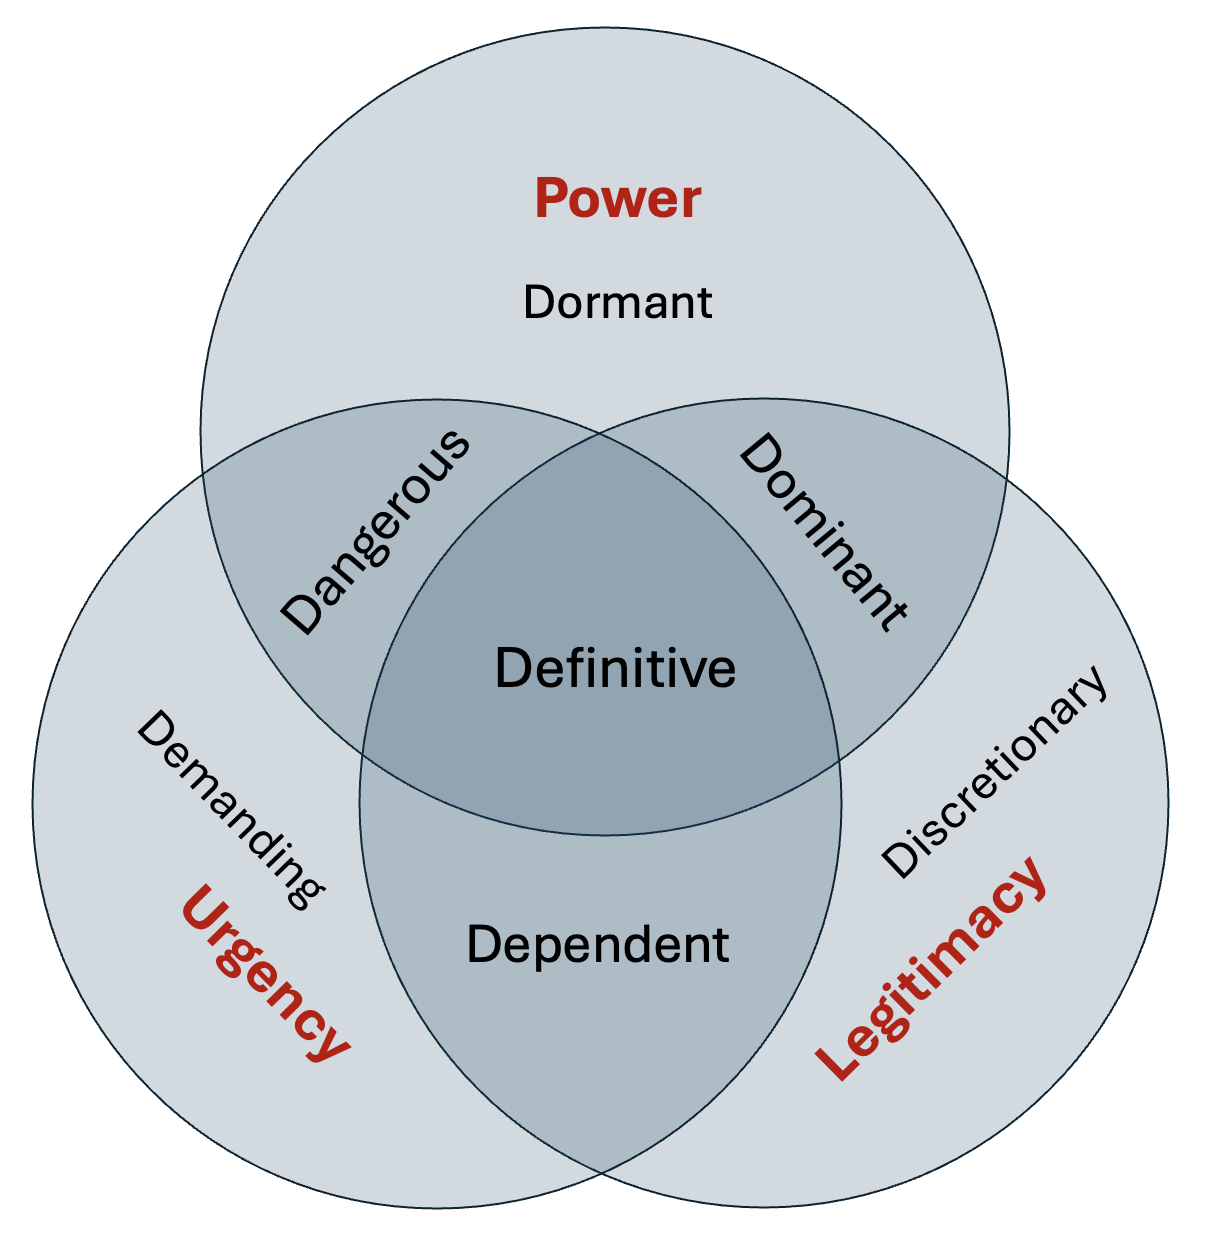
\includegraphics[width=0.6\textwidth]{figures/StakeholderVennDiagram.png}
\caption{Redrawn Stakeholder Typology from Mitchell Stakeholder Salience Model \cite{mitchell_1997} applied to the CAM testing ecosystem.}
\label{fig:stakeholder_salience_typology}
\end{figure}

While traditional matrices (such as RACI) map static responsibilities, the high-risk CAM sector demands a dynamic framework for prioritisation. The Mitchell et al. Stakeholder Salience Model \cite{mitchell_1997} captures rapid, event-driven shifts and focuses engagement on actors possessing two or more attributes. The model uses the triad of power, legitimacy, and urgency (Figure~\ref{fig:stakeholder_salience_typology}).

In accordance with Proposition 1a, which asserts that ``stakeholder salience will be low where only one of the stakeholder attributes (power, legitimacy, and urgency) is perceived by managers to be present'' \cite[p.~874]{mitchell_1997}, this report focuses its active engagement strategy on stakeholders possessing two or more of these attributes.

For every such class, the applicable stakeholders are given and the reasoning is explained:

\begin{itemize}
    \item Definitive Stakeholders - Insurers \& testbed operators: These actors possess all three attributes. Insurers hold financial power and legal legitimacy over operations, while their need for immediate post-incident data drives high urgency. Similarly, testbed operators have the power and legitimacy to halt trials instantly to protect track infrastructure and personnel.
    \item Dominant Stakeholders - Regulators \& highway authorities: Entities such as CCAV hold ultimate regulatory power and legitimacy; under Mitchell's theory, their urgency is typically event-driven and only spikes post-incident, provided compliance is maintained \cite[p.~874]{mitchell_1997}.
    \item Dependent Stakeholders - General public: This group holds high moral legitimacy and urgency regarding physical safety, but lacks direct power to enforce testing protocols, relying instead on internal ethics governance.
    \item Dangerous Stakeholders - Cyber-threat actors: While these actors possess no legitimacy, they have both power and urgency to maliciously obtain valuable data or disrupt the service the enterprise offers to competitors.
\end{itemize}

\subsection{Applying the model}

For each stakeholder mentioned above, the salience class, value exchange, and compliance mechanism (split between the R\&D and commercial phases where relevant) are given in Table~\ref{tab:strategic_engagement_matrix}.

\begin{table}[htbp]
\centering
\small
\setlength{\tabcolsep}{3pt}
\renewcommand{\arraystretch}{1.15}
\caption{Strategic Engagement and Value Exchange Matrix}\label{tab:strategic_engagement_matrix}
\begin{tabular}{|>{\raggedright\arraybackslash}p{0.12\linewidth}|>{\raggedright\arraybackslash}p{0.14\linewidth}|>{\raggedright\arraybackslash}p{0.22\linewidth}|>{\raggedright\arraybackslash}p{0.26\linewidth}|>{\raggedright\arraybackslash}p{0.14\linewidth}|}
\hline
\textbf{Stakeholder Group} & \textbf{Salience Class} & \multicolumn{2}{c|}{\textbf{The Value Exchange}} & \textbf{Compliance Mechanism} \\
\cline{3-4}
 & & \textbf{Need} & \textbf{Solution} & \\
\hline
Testbed Operators & Definitive in R\&D & Guarantee that the experimental prototype will not destroy track infrastructure. & Extreme transparency and rigorous safety mitigation plans. & PAS~1881 \cite{pas1881} (Safety governance) \\
\cline{2-5}
 & Definitive in Commercial & Attract top AV developers to rent their tracks. & We provide a highly integrated, value-add service that brings clients directly to their facility. & Operational resilience (spares/SLA) \\
\hline
AV Start-ups \& OEMs & Discretionary (Latent) in R\&D & Assurance that the conceptual target will meet their AI requirements. & Market-fit validation and technical alignment. & PAS~1883 \cite{pas1883} (ODD Taxonomy) \\
\cline{2-5}
 & Definitive in Commercial & Capital-efficient, rapid edge-case validation. & We absorb CAPEX and hardware maintenance, delivering on-demand testing data. & Contracted evidence deliverables \\
\hline
Component Suppliers & Definitive in R\&D & Proof of engineering viability for custom parts. & Custom tuning feedback and baseline component testing. & Engineering Service Legal Agreements \\
\cline{2-5}
 & Dominant (Urgency drops) in Commercial & Predictable, high-volume recurring revenue. & Long-term purchase orders to maintain our modular inventory buffer. & PAS~1881 \cite{pas1881} (Maintenance governance) \\
\hline
Insurers \& Investigators & Definitive & Irrefutable proof of liability during and after collisions. & We absorb the ambiguity of crashes by acting as an incorruptible data proxy. & PAS~1882 \cite{pas1882} (Evidence trail) \\
\hline
Regulators (e.g., CCAV) & Dominant & Proof that autonomous systems are reaching ALARP safety standards. & We provide the physical scenario-testing required to generate their safety metrics. & PAS~1881 \cite{pas1881} (Safety case) \\
\hline
The Public \& VRUs & Dependent & Protection from immature, dangerous AV technology. & We act as their proxy, absorbing the physical impacts of edge-case testing. & Ethics and legitimacy \\
\hline
Cyber-Threat Actors & Dangerous & Goal: Exploit systemic vulnerabilities for disruption or hijacking. & Mitigation: Defensive shielding and encrypted telemetry to ensure testing integrity. & PAS~1885 \cite{pas1885} (Cyber controls) \\
\hline
\end{tabular}
\end{table}

\subsection{Continuations to the model}

While Table~\ref{tab:strategic_engagement_matrix} maps salience, it is important to distinguish the structural nature of power. Actors such as CCAV, Thatcham Research, and BSI operate as ``stakekeepers'' \cite[p.~121]{fassin_2009}: independent regulatory and certification bodies with legitimacy and the ability to dictate market access. Their requirements therefore become foundational operational constraints.

The enterprise treats these attributes not as binary states, but as a continuum. Latent groups are subjected to continuous passive monitoring to ensure we anticipate any escalation in their urgency or power before they cross the threshold into definitive threats.

\noindent\textbf{Implication:} commercial success depends not only on paying customers, but also on stakeholders who control legitimacy and access, especially testbed operators, insurers, and regulators.

\section{Execution plan for stakeholder acceptance}
\label{sec:stakeholder_acceptance_execution_plan}

This first-year execution plan converts the salience analysis into practical acceptance. In this market, stakekeepers (testbed operators, regulators, and insurers/investigators) gate market access (Table~\ref{tab:strategic_engagement_matrix}), so success depends on evidence quality, safety governance, and operational uptime.

\begin{table}[htbp]
\centering
\small
\setlength{\tabcolsep}{3pt}
\renewcommand{\arraystretch}{1.15}
\caption{Stakeholder acceptance roadmap (Year 1): deliverables, value capture, \& acceptance gates.}
\label{tab:stakeholder_engagement_roadmap}
\begin{tabular}{|>{\raggedright\arraybackslash}p{0.17\linewidth}|>{\raggedright\arraybackslash}p{0.34\linewidth}|>{\raggedright\arraybackslash}p{0.28\linewidth}|>{\raggedright\arraybackslash}p{0.15\linewidth}|}
\hline
\textbf{Stakeholder (salience)} & \textbf{Engagement activity \& deliverable} & \textbf{Value captured (why TaaS)} & \textbf{Acceptance gate} \\
\hline
Testbed operator (Definitive $\rightarrow$ Essential) & Safety induction and operating-envelope sign-off; E-stop drills; recovery procedure and spares plan. & Higher utilisation; de-risked on-site operations without building their own target capability. & Pilot slot granted; operator sign-off \\
\hline
Regulator / authority (Dominant $\rightarrow$ Essential) & Safety case pack (hazard log, SOPs, change control) and controlled-trial briefing pack. & Empirical support beyond simulation-only validation; comparable evidence across trials. & No-blocker feedback for controlled trials \\
\hline
Insurer / investigator (Definitive $\rightarrow$ Essential) & Telemetry access protocol (``black box'' logging) and investigator-ready incident package template (data, timeline, deviations). & Clear attribution evidence for pricing and liability decisions from independent telemetry. & Agreement logs support attribution \\
\hline
Suppliers (Definitive $\rightarrow$ Essential) & Modular BOM; spares strategy; lead-time risk register; refurbishment loop definition. & Predictable spares and refurbishment demand; clear requirements reduce integration risk. & Availability and turnaround agreed \\
\hline
OEM / AV developer (Latent $\rightarrow$ High) & Scenario catalogue; repeatability report format; clear ODD boundaries for each test day. & Pay-per-use edge-case validation without CAPEX or maintaining a target fleet. & Paid pilot or LOI \\
\hline
Public / VRUs (Dependent $\rightarrow$ Supporting) & Plain-language rationale for off-public-road edge-case testing; evidence-first posture. & Reduced exposure to public-road trials; legitimacy from an evidence-first safety posture. & No reputational blocker \\
\hline
\end{tabular}
\end{table}

This roadmap makes value capture explicit: customers buy validated evidence and repeatability, testbeds gain utilisation, regulators and insurers gain credible assurance data, and the enterprise gains recurring revenue only if acceptance gates are met.

\subsection{Operational success metrics}

The following metrics are reported monthly to provide early warning of safety, evidence-quality, and uptime failures that would otherwise undermine testbed acceptance and utilisation.

\begin{itemize}
    \item \textbf{Safety:} incident-free test days; near-miss rate; time-to-stop performance in E-stop drills.
    \item \textbf{Evidence quality:} percentage of runs with complete logs and scenario metadata; time to produce an investigator-ready run package.
    \item \textbf{Uptime:} mean time to recover after contact; unplanned downtime versus utilisation breakpoints in the financial model.
    \item \textbf{Commercial traction:} conversion from pilot discussions to paid pilots/contracts; repeat booking rate; blended day-rate trend.
\end{itemize}

\noindent\textbf{Implication:} the first-year execution plan must prioritise stakeholder acceptance before scale, because without testbed approval, evidence credibility, and operational uptime, the service cannot reach commercial deployment.

\section{Stakeholder Acceptance Personas}
\label{sec:paul_personas}

These personas are not intended to repeat the customer personas in Section~\ref{sec:personas}. Instead, they represent adoption gatekeepers whose approval determines whether the TaaS model can operate commercially within the UK CAM ecosystem.

\subsection{The CAM Testbed Operations Director (The Partner)}

\textit{Context: Facility leadership at a state-backed testing ground, such as UTAC Millbrook-Culham}.

\textbf{Role:} Director of Track Operations and Commercial Partnerships.

\textbf{Motivations \& End Goals:} Evaluated strictly on track utilisation metrics and facility safety records. Their primary goal is to attract tier-1 AV developers by offering the most reliable, cutting-edge physical testing infrastructure in Europe.

\textbf{Pains:} Unpredictable, bespoke test-target suppliers. When a client's custom testing dummy shatters during a high-speed impact, the track must be shut down for hours to clear hazardous debris. This destroys the daily testing schedule, forces the facility to issue refunds for lost time, and artificially caps their revenue.

\textbf{Decision Influence \& Value Exchange:} Controls the "approved vendor" list for the facility. By exclusively partnering with our TaaS platform, they guarantee their clients rapid trackside recovery times. Furthermore, by transferring operational liability to our safety staff trained to PAS 1884-informed operating expectations \cite{pas1884}, we directly boost their facility's daily throughput and derisk their commercial operations, making us an indispensable embedded supplier.

\subsection{The Independent Liability Assessor (The Gatekeeper)}

\textit{Context: Technical safety auditor for an insurance intelligence body (e.g., Thatcham Research) or government regulator (e.g., CCAV)}.

\textbf{Role:} Lead Risk Analyst for Automated Driving Systems (ADS).

\textbf{Motivations \& End Goals:} Tasked with establishing legal fault in simulated edge-case crashes to build the foundation for commercial insurance policies. They need empirical, unassailable data to verify that a system has met the "as low as reasonably practicable" (ALARP) safety threshold before certifying it for public roads.

\textbf{Pains:} Competing narratives during track incidents. AV developers often blame testing equipment or track conditions for edge-case failures rather than their own algorithms. This ambiguity makes it impossible for assessors to confidently price risk premiums or assign legal liability.

\textbf{Decision Influence \& Value Exchange:} Holds the ultimate veto over a vehicle's public road certification. By utilising our dummy vehicle's Electronic Control Unit (ECU) to produce a tamper-evident evidence trail aligned with PAS 1882-style expectations \cite{pas1882}, our platform provides them with an incorruptible, third-party "black box." We deliver objective telemetry that is completely independent of the OEM, solving their core data-integrity problem and incentivising them to mandate our platform for future Operational Safety Cases.

\section{Integrated Strategy for Ethics, Liability, and Safety Assurance}

The UK Automated Vehicles Act 2024 fundamentally shifts legal liability away from human drivers and onto the corporate developers \cite{lawcom_avs_2024}. In this environment, ethical obligations, legal liability, and safety assurance cannot be treated as isolated topics; they are inextricably linked. Our strategy navigates this complex web by positioning our hardware as the critical compliance tool across three integrated fronts:

\subsection{The Ethical Safety Buffer}

The industry faces a moral imperative to deploy life-saving AV technology, but high-speed validation testing introduces severe risks. PAS 1881-style expectations require that public welfare is protected and operational risks are reduced to a level that is "as low as reasonably practicable" (ALARP) \cite{pas1881}.

Our testing platform serves as an ethical and safety buffer. By enabling hazardous fault injection and edge-case validation within strictly defined Operational Design Domains (ODD) specified using PAS 1883 taxonomy \cite{pas1883}, the service absorbs physical risk in controlled environments rather than on public roads. This supports PAS 1881-style ethical impact assessment and safety governance \cite{pas1881} while lowering barriers to credible testing.

\subsection{Liability Demarcation through Data Transparency}

Under the UK Law Commission's framework, clients (as ASDEs) assume legal responsibility for dynamic driving behaviour when the automated driving system (ADS) is engaged \cite{lawcom_avs_2024}. During physical edge-case validation, collisions can be an expected outcome, so insurers and investigators require unhindered access to telemetry \cite{thatcham_2026}. The dummy vehicle's Electronic Control Unit (ECU) therefore provides continuous, high-fidelity logging intended to be compatible with PAS 1882-style evidence requirements \cite{pas1882}. Acting as a tamper-evident ``black box'', this transparency supports clear liability demarcation when the equipment operates within defined parameters.

\subsection{Algorithmic Bias, Cybersecurity, and Continuous Learning}

Safety and legal compliance are not static achievements. As testbeds and vehicles become interconnected, insurers and regulators highlight systemic vulnerabilities such as algorithmic bias and cyber-threats.

While the enterprise does not develop client AI algorithms, it is responsible for the physical environments used to validate them. A critical vulnerability is algorithmic "overfitting", where systems are trained only against predictable traffic patterns and uniform vehicle shapes. The platform therefore governs physical scenario curation by deploying modular target shells that span vehicular geometries and high-dynamic behaviours, avoiding an artificially sanitised validation environment. This supports the UK Law Commission’s (2022) mandate that ASDEs must prove safe and legal driving across foreseeable traffic conditions before public deployment \cite[pp.~49, 81--82, 87]{lawcom_2022} and strengthens PAS 1881-style safety case expectations \cite{pas1881}.

To protect systemic integrity, the platform should be informed by PAS 1885 \cite{pas1885} cybersecurity principles, using encrypted communication to reduce the risk of unauthorised modification or remote hijacking.

Finally, these elements are governed by a Safety Management System (SMS) designed with reference to PAS 1881 \cite{pas1881}. Treating safety cases as "live documents" ensures near-misses and unexpected component behaviours feed into change control for continuous improvement.

\section{Sustainability, Lifecycle, and the Circular Economy}

Sustainability is treated here as a strategic consequence of the TaaS model rather than as a separate design topic. Because the enterprise retains ownership of the vehicle fleet, environmental incentives and commercial incentives become aligned: longer asset life, repairability, recyclability, and reduced redundant manufacturing all improve both sustainability and margin resilience.

In the automotive sector, Life Cycle Assessments (LCA) often emphasise tailpipe emissions and grid mix. For an electric TaaS platform, the use-phase is effectively zero-emission, so sustainability pivots to manufacturing impacts: almost half of an EV's life cycle Global Warming Potential (GWP) is locked into production \cite[p.~56]{hawkins_2013}. The report therefore mandates "effective recycling programs and improved EV lifetimes" \cite[p.~61]{hawkins_2013}. The enterprise operationalises this through a Product-Service System (PSS) framework (life extension) and the 9R Circular Economy framework (closed-loop recycling), reducing the environmental impact of autonomous validation toward ALARP.

\subsection{Product-Service Systems (PSS) Framework}

At the macro-business level, the TaaS model is a Result-Oriented Product-Service System (PSS), aligning with Activity Management and Outsourcing (Category 6) \cite[p.~254]{tukker}. Centralising this service at UK testbeds reduces redundant material extraction by avoiding multiple low-utilisation client fleets.

\subsection{The 9R Framework Application}
\label{sec:9r_framework_application}

To achieve absolute alignment between environmental sustainability and commercial efficiency, the enterprise governs its lifecycle strategy through the 9R Circular Economy Framework \cite[p.~5]{potting_2017}. Because asset ownership is retained under the TaaS model, we are financially incentivised to maximise hardware lifespan. At the macro-level, this overarching Product-Service System (PSS) successfully executes the framework's highest tiers: Smarter product use and manufacture (R0-R2) by refusing redundant OEM manufacturing and reducing overall material extraction across the industry.

However, at the micro-level, we face a critical engineering constraint: the reliance on the foundational Formula Student (FS) vehicle architecture. Because the base chassis and drivetrain materials are predetermined by this inherited design, the enterprise cannot optimise the platform's initial embodied carbon. To counter this, we deploy a modular hardware strategy designed to keep inherited materials at their highest utility despite the intense mechanical stress and frequent collisions of track testing. Consequently, our hardware management is categorised across three core subsystems, mapping directly to the framework's subsequent mandates to Extend lifespan (R3-R7) and ensure the Useful application of materials (R8-R9):

\begin{itemize}
    \item Energy Storage (Extend Lifespan: R3 Reuse \& R7 Repurpose): The inherited design provides a massive environmental advantage by utilising a supercapacitor architecture rather than traditional Lithium-ion battery packs, which rely on heavily mined rare-earth metals and suffer high chemical degradation under extreme discharge rates. Supercapacitors possess an exceptional cycle life and low degradation under high power cycling compared to other feasible solutions (detailed in Section~\ref{sec:technology_selection} and Figure~\ref{fig:supercap_discharge}).
    \item The Drivetrain \& Chassis (Extend Lifespan: R4 Repair, R5 Refurbishment \& R6 Remanufacture): The platform will be subjected to intense mechanical stress through high-dynamic testing. By adopting a modular supply chain, high-value inherited components (such as electric motors and suspension linkages) can be managed through rigorous refurbishment and remanufacturing loops (R5/R6). Furthermore, the steel spaceframe allows for track-side welding and repair (R4), extending the life of the asset indefinitely and preventing the need to commission an entirely new chassis after minor track incidents. Consequently, in both the drivetrain and the chassis, sustainability is actively achieved through operational lifecycle extension.
    \item The Sacrificial Shell (Useful Application of Materials: R8 Recycle): The most significant hardware update to our initial design is the external target shell, our highest-wear component. The strategic plan explicitly rejects rigid composites, like carbon fibre, which utilise thermoset plastics. This material not only makes the component difficult to sustainably recycle, with the vast majority sent to landfills \cite[p.~2]{morici_2022}, but also introduces hazardous track debris through shattering. Instead, the enterprise specifies the use of Recycled Expanded Polypropylene (rEPP), which is a highly impact-absorbent, low-cost, and lightweight thermoplastic foam, already used in automotive pedestrian protection applications \cite[p.~1]{ramaswamy_2017}. Following a track collision, the shattered EPP shells can be cleanly collected, melted down, and re-extruded into brand new impact shells, establishing a perfectly closed, 100\% recyclable material loop (R9) (demonstrated in \cite{handtke_2024}).
\end{itemize}

\noindent\textbf{Implication:} sustainability is not a separate reputational claim; it reinforces the economics of TaaS because asset ownership incentivises repair, reuse, refurbishment, and high utilisation.

\section{Strategic Limitations \& Cross-Functional Dependencies}

The following limitations are not isolated risks within the strategy function. They are cross-functional dependencies that determine whether the TaaS model is commercially viable. Financial exposure is tested through the financial model (Sections~\ref{sec:breakeven} and \ref{sec:downtime}), operational resilience is developed through the supply-chain plan (Section~\ref{sec:supply_chain_planning}), and minimum viable safety is addressed through prototype planning (Chapter~\ref{chap:eem_prototype_planning}).

While the TaaS model addresses the simulation-to-reality gap, it introduces internal vulnerabilities that must be managed through engineering and financial integration.

\subsection{Financial Exposure and Capital Intensity}

While TaaS shifts client costs to OPEX, the primary limitation is the inversion of enterprise capital expenditure (CAPEX). The enterprise must fund fleet manufacture, infrastructure, and insurance before revenue begins. Solvency therefore depends on achieving the minimum utilisation rates implied by Sections~\ref{sec:breakeven} and \ref{sec:downtime}.

\subsection{Asset Ownership and the Maintenance Bottleneck}

Under the PSS framework, retained ownership transfers hardware failure risk to the enterprise. Because revenue is tethered to uptime, collision damage that exceeds forecast repair windows erodes margins and can threaten testbed relationships. Commercial execution therefore depends on Supply Chain Planning (Section~\ref{sec:supply_chain_planning}), including modular spares buffers and trackside recovery protocols.

\subsection{The Regulatory "Cold Start" Problem}

Finally, integrating into established CAM Testbed UK facilities creates a regulatory "cold start" problem. Operations directors and liability assessors (stakekeepers) require empirical proof that the platform will not damage infrastructure or endanger personnel, but this evidence is difficult to generate without track access. The mitigation is staged proof-of-concept testing aligned to Chapter~\ref{chap:eem_prototype_planning} (Design Requirements \& Prototype Planning), ensuring the platform reaches minimum viable safety thresholds required for initial approval.

The minimum viable strategic conditions for the TaaS model are therefore: first, at least one CAM testbed must approve controlled pilot operation; second, telemetry and incident evidence must be credible to insurers, regulators, and customers; third, paid pilots must convert into repeat bookings; fourth, utilisation must approach the break-even threshold identified in the financial model (Section~\ref{sec:breakeven}); and fifth, downtime must remain within the recovery assumptions supported by the supply-chain plan (Section~\ref{sec:supply_chain_planning}). If any of these conditions fail, the strategy should be narrowed before further fleet expansion.

\noindent\textbf{Implication:} the strategy is only commercially defensible if the operational recovery assumptions and financial utilisation thresholds in later chapters are realistic.

% --- END INLINE: PaulVogelberg/Business/paul_business_body.tex ---
\vspace{6pt}
\compactbib
\end{refsection}

\begin{refsection}
\graphicspath{{../MichaelZiyangXing/}}
% --- BEGIN INLINE: MichaelZiyangXing/eem_design_requirements_prototype_planning_compact.tex ---
% -----------------------------------------------------------------------------
% Compact preliminary EEM draft section for internal team review
% Project: UK-focused AEB test-carrier development from baseline EV chassis
% Target length: approximately 14--15 pages with styling.sty, figures, and references
% -----------------------------------------------------------------------------

\chapterauthor{Commercially Driven Design Requirements and Prototype Planning}{Ziyang Xing}
\label{chap:eem_prototype_planning}
\contribution{This chapter frames the design requirements and prototype plan for the autonomous emergency braking (AEB) test carrier from an Engineering Entrepreneurship and Management (EEM) perspective. It links technical requirements to UK customer needs, standards-led testing expectations, prototype-risk reduction, and commercialisation logic.}

\section{Purpose and commercial framing}

This chapter evaluates the design requirements and prototype plan for converting the team's baseline product, a lightweight and configurable electric vehicle (EV) chassis, into a high-dynamics autonomous emergency braking (AEB) test carrier. The proposed product direction is to prioritise vehicle-to-vehicle (V2V) AEB test cases, while retaining compatibility with less demanding tests such as pedestrian, cyclist, and low-speed obstacle scenarios. The design problem is therefore not only whether the vehicle can accelerate, brake, and follow a controlled path. It is whether these technical capabilities can become a credible and commercially useful testing asset for UK original equipment manufacturers (OEMs), proving grounds, connected and automated mobility (CAM) testbeds, advanced driver assistance system (ADAS) developers, and research organisations.

The chapter treats design requirements as market-facing requirements. Physical performance requirements determine which test cases the carrier can support. Experimental setup requirements determine whether the evidence produced is repeatable and usable. Standards and data requirements determine whether the prototype is credible in a professional UK testing environment. The prototype roadmap then shows how the team can begin with a low-cost exploratory platform, validate repeatability, demonstrate high-dynamics V2V capability, and finally package the system as a customer-ready demonstrator. This structure follows good practice observed in previous EEM project reports: clear customer segmentation, UK ecosystem framing, disciplined treatment of assumptions and financing, and operational realism around maintainability and downtime.

The scope is deliberately limited to the UK. EU and US regulatory pathways, including NHTSA-oriented expansion, are treated as future commercial scaling opportunities rather than immediate design drivers. This is appropriate for the current report because it keeps the design argument focused on UK customers, UK trial expectations, and relevant British Standards Institution (BSI) PAS documents. The central argument is that the test carrier should not be designed as a generic fast remote-controlled vehicle. It should be designed as a standards-aware, repeatable, data-producing test object that can support a future testing service or equipment offering.

\textbf{TODO: CONFIRM PROJECT-SPECIFIC SCOPE.} This draft assumes that the baseline EV chassis is available as a functioning or near-functioning platform and that the agreed market entry point is a high-dynamics AEB test carrier rather than a full autonomous driving vehicle. Before submission, this paragraph should be updated with the actual chassis status, the ownership of the baseline design, and the boundary between this EEM chapter and the engineering-design chapter.

\section{UK market need and customer problem}

\subsection{Why a physical AEB test carrier is useful}

AEB development increasingly uses simulation, software-in-the-loop testing, and controlled proving-ground experiments. Simulation is efficient for exploring large numbers of scenarios, but it cannot fully replace physical testing where perception, timing, actuation, tyres, surface condition, target presentation, and near-collision safety interact. For a customer, the value of a physical test carrier is therefore not only the vehicle itself. The value lies in producing repeatable, believable, and traceable evidence under controlled conditions.

The commercial opportunity sits between two extremes. Low-cost prototype platforms can be built quickly, but they often lack repeatability, data quality, safety documentation, and customer confidence. Premium active-safety test systems offer high capability, but they can be expensive, specialised, and difficult for smaller developers or research-led teams to access. The proposed AEB test carrier should occupy an intermediate position: a modular, lower-cost, UK standards-aware platform that first proves serious V2V testing capability and then matures towards a professional demonstrator.

\textbf{TODO: COLLECT MARKET EVIDENCE.} The final report should add at least two concrete evidence sources, such as stakeholder interviews, indicative supplier prices, published testbed-access rates, or CAM-sector reports. If exact costs cannot be obtained, the analysis should clearly state that it uses indicative cost bands rather than verified supplier quotations.

\subsection{Customer segments}

The first UK-focused commercialisation phase should target business-to-business customers rather than private consumers. The most relevant users are organisations that need to generate, validate, or sell AEB test evidence. Table~\ref{tab:customer_segments_compact} summarises the customer segments and their design implications.

\begin{table}[H]
\centering
\caption{Indicative UK customer segments and design implications.}
\label{tab:customer_segments_compact}
\begin{tabular}{p{0.20\textwidth} p{0.31\textwidth} p{0.37\textwidth}}
\toprule
\textbf{Segment} & \textbf{Primary need} & \textbf{Design implication} \\
\midrule
OEM validation teams & Repeatable V2V AEB evidence for internal development. & Prioritise acceleration, braking repeatability, trajectory control, logging, and reportable outputs. \\
\midrule
Proving grounds and CAM testbeds & Additional active-safety service capability. & Prioritise robust operation, fast reset, safety procedures, maintainability, and workflow integration. \\
\midrule
ADAS developers and Tier suppliers & Faster iteration between software changes and physical tests. & Prioritise modular scenarios, accessible data export, and lower operating cost. \\
\midrule
Research organisations & Affordable platform for controlled safety experiments. & Prioritise safe operating limits, instrumentation access, and transparent limitations. \\
\bottomrule
\end{tabular}
\end{table}

The shared customer problem is access to controlled physical validation without immediately taking on the full cost, complexity, and liability burden of premium target fleets. This makes the prototype plan commercially important. The team must not simply maximise technical ambition; it must decide which capabilities create customer confidence at each stage of development.

\subsection{UK policy and standards context}

The UK context strengthens the rationale because connected and automated mobility is an active national policy and investment area. The Automated Vehicles Act 2024 creates a legal framework for automated vehicles in Great Britain, while UK Government and CAM Testbed UK material presents automated mobility as a growth sector and testbed opportunity \parencite{automatedVehiclesAct2024,govukAVJobs2025,camTestbedUK}. The project should not claim that a university prototype is immediately compliant with commercial certification requirements. Instead, UK policy and standards should be used as design guidance: they show what a serious testing platform will eventually need to demonstrate.

For this report, the most relevant UK-facing references are PAS 1881 for operational safety, PAS 1882 for data collection and incident-investigation readiness, PAS 1883 and BS ISO 34503 for Operational Design Domain (ODD) definition, the Department for Transport automated vehicle trialling code of practice, ISO 22133 for test-object monitoring and control, and the ISO 19206 series for surrogate targets \parencite{bsiPAS1881,bsiPAS1882,bsiPAS1883,iso34503,dftTriallingCode,iso22133,iso19206series}. These sources do not all apply in the same way, but together they justify three design priorities: safe operation, repeatable tests, and traceable evidence.

\textbf{TODO: VERIFY VERSION-SENSITIVE STANDARDS.} Some standards are version-sensitive. Before submission, the team should confirm the exact current versions available through the university or BSI access, especially PAS 1881, PAS 1883, and ISO 22133. The report should avoid claiming formal compliance unless the corresponding evidence has been generated.

\begin{table}[H]
\centering
\caption{UK-focused standards and design implications.}
\label{tab:standards_design_compact}
\begin{tabular}{p{0.25\textwidth} p{0.61\textwidth}}
\toprule
\textbf{Reference} & \textbf{Implication for the AEB test-carrier project} \\
\midrule
PAS 1881 & Motivates safety-case thinking, operating limits, emergency procedures, change control, and monitoring of safety assumptions. \\
PAS 1882 & Motivates structured data capture, data retention, incident review, access control, and evidence preservation. \\
PAS 1883 / BS ISO 34503 & Motivates a clearly defined ODD for the prototype, including test environment, surface, speed range, target type, and weather limits. \\
DfT trialling guidance & Reinforces safety management, competent supervision, and responsible operation during public or semi-public trials. \\
ISO 22133 / ISO 19206 & Supports compatibility with active-safety test-object control and surrogate target expectations. \\
\bottomrule
\end{tabular}
\end{table}

\section{Design requirements as commercial requirements}

\subsection{Requirement logic}

The design requirements are organised into three lenses: physical performance, experimental setup, and standards/data readiness. This avoids presenting the carrier as a collection of unrelated technical specifications. Each lens answers a customer-facing question. First, can the platform execute the test cases that customers value? Second, can it repeat those tests reliably enough for engineering evidence? Third, can it produce data and documentation that a professional customer can trust?

\begin{table}[H]
\centering
\caption{Commercial interpretation of key design requirements.}
\label{tab:requirements_compact}
\begin{tabular}{p{0.18\textwidth} p{0.31\textwidth} p{0.24\textwidth} p{0.17\textwidth}}
\toprule
\textbf{Lens} & \textbf{Key points} & \textbf{Customer value} & \textbf{Example target} \\
\midrule
Physical performance & Acceleration, braking, top speed, payload, low-profile structure, and target compatibility. & Enables higher-value V2V AEB cases rather than only low-speed target motion. & 0--X km/h in $<$ X s; decel $>$ X m/s$^2$. \\
\midrule
Experimental setup & Repeatable speed, path, heading, scenario reset, emergency stop, and run-to-run consistency. & Reduces wasted test time and increases confidence that measured differences are caused by the vehicle under test. & Speed error $<$ $\pm$X km/h; lateral error $<$ $\pm$X m. \\
\midrule
Standards and data & Synchronised logging, scenario metadata, incident records, operating limits, and traceable reports. & Converts a moving carrier into professional test evidence. & Logging $>$ X Hz; time sync error $<$ X ms. \\
\bottomrule
\end{tabular}
\end{table}

\subsection{Physical performance}

The physical-performance requirements determine whether the platform can credibly support the chosen market position. A pedestrian-only target carrier can be relatively low speed and low acceleration, but V2V AEB scenarios require stronger longitudinal performance, stability, and control. The carrier should therefore be designed around measurable targets such as 0--X km/h acceleration time, maximum test speed of X km/h, braking deceleration above X m/s$^2$, payload capacity of X kg, and safe operation with a soft vehicle target mounted or towed.

These figures should not be treated as arbitrary engineering ambitions. They are commercial filters. If the chassis cannot reach the required dynamics, it may still be useful for low-speed research, but it will not support the differentiated value proposition of high-dynamics V2V AEB testing. Conversely, over-specifying the vehicle too early would increase cost before demand is validated. The correct approach is to define minimum performance thresholds for each prototype stage and tighten them only after early tests show the chassis can support further development.

\textbf{TODO: INSERT ACTUAL PERFORMANCE TARGETS.} Replace X values with measured or justified targets from the engineering team. The final report should state whether each target is an aspiration, a calculated requirement, or a measured prototype result.

\subsection{Experimental setup and repeatability}

Repeatability is the bridge between a technical prototype and a test product. The carrier must be able to execute the same scenario multiple times with controlled variation in speed, path, heading, acceleration, and timing. This is commercially important because testbed operators sell reliable test time. If the platform requires long manual setup, has high downtime, or produces inconsistent runs, its commercial value falls even if the hardware is impressive.

The experimental requirements should therefore include both test-quality and operational metrics. Test-quality metrics include path error below $\pm$X m, speed error below $\pm$X km/h, heading error below $\pm$X degrees, and repeatability over X repeated runs. Operational metrics include reset time below X minutes, number of runs per charge above X, repair time after minor contact below X minutes, and number of staff required per test day. These operational details connect engineering decisions to the EEM criteria because they affect cost, utilisation, and customer satisfaction.

\subsection{Standards, data, and evidence quality}

The standards/data lens converts motion into evidence. The platform should record sufficient data to reconstruct each run and explain the test context. A preliminary data-channel set should include timestamp, position, velocity, acceleration, yaw or heading, drive command, braking command, energy-store state, communications status, emergency-stop status, fault codes, scenario ID, operator, software version, weather condition, and any deviations from the planned test.

The logging frequency should be selected according to the fastest dynamics that need to be captured. In this draft, X Hz is used as a placeholder; the team should decide whether 100 Hz is technically achievable and commercially necessary for the later prototype. The report should be careful with wording. It can say that the data architecture is designed with standards-aware logging in mind, but it should not claim compliance until the sensors, synchronisation, storage, calibration, and data-processing chain have been validated.

\textbf{TODO: CONFIRM DATA ARCHITECTURE.} The final report should specify which channels are recorded at high frequency, which are recorded at lower frequency, how time synchronisation is achieved, and how raw logs are converted into customer-facing reports. If the early prototype cannot achieve the final logging target, present this as a staged limitation rather than a failure.

\section{Prototype roadmap: Explore, Validate, Demonstrate, Convince}
\label{sec:prototype_roadmap_compact}

\subsection{Why staged prototyping is necessary}

The project begins with limited resources, uncertain customer demand, and unverified technical performance. A single attempt to build a customer-ready product from the beginning would create high financial and technical risk. A staged roadmap reduces this risk by creating decision gates. Each stage answers a clear question: can the chassis move safely; can it repeat a controlled test; can it demonstrate high-dynamics V2V value; and can it produce evidence that customers would trust?

\begin{figure}[H]
\centering
\fbox{\parbox{0.86\textwidth}{\centering\vspace{7mm}
\textbf{PLACEHOLDER FOR ROADMAP FIGURE}\par
A compact vertical figure should show: P0 Explore $\rightarrow$ P1 Validate $\rightarrow$ P2 Demonstrate $\rightarrow$ P3 Convince. Each stage should contain two or three short phrases. The style should match the dark-blue presentation theme.\vspace{7mm}}}
\caption{Staged prototype path from low-cost exploration to customer-ready proof.}
\label{fig:prototype_roadmap_compact}
\end{figure}

\subsection{Stage definitions}

P0, \textit{Explore}, should use the baseline EV chassis with the minimum modifications required for safe controlled motion. The purpose is to learn cheaply, not to impress customers. The expected evidence includes simple acceleration traces, braking traces, emergency-stop tests, video records, and operator feedback. If the chassis cannot meet a minimum motion envelope at P0, the team can pivot before investing in expensive sensors or target structures.

P1, \textit{Validate}, should convert the moving chassis into a repeatable experimental platform. The main additions are closed-loop velocity control, improved position or heading estimation, structured scenario setup, and reliable logging. The output should be a repeatability evidence pack showing, for example, that the vehicle can run a planned path at X km/h with speed error below $\pm$X km/h and lateral error below $\pm$X m over X repeated runs.

P2, \textit{Demonstrate}, should show the differentiated value proposition: high-dynamics V2V AEB testing. This stage should add soft vehicle target integration, a priority scenario library, stronger safety supervision, and enough performance to execute commercially interesting cases. Candidate cases include stationary target approach, moving target approach, braking target, crossing target, or low-speed cut-in scenarios. The exact scenario set should be chosen to match both customer interest and safe technical capability.

P3, \textit{Convince}, should package the prototype into a customer-ready demonstrator. This does not necessarily mean full commercial certification. It means that the prototype has the artefacts needed for a serious pilot discussion: operating manual, risk assessment, safety-case outline, scenario catalogue, data-export format, report template, maintenance plan, and costed service model. At this stage, the aim is not merely to show that the vehicle is fast; it is to reduce customer uncertainty.

\begin{table}[H]
\centering
\caption{Prototype stages, evidence outputs, and business decisions.}
\label{tab:prototype_stages_compact}
\begin{tabular}{p{0.14\textwidth} p{0.25\textwidth} p{0.29\textwidth} p{0.20\textwidth}}
\toprule
\textbf{Stage} & \textbf{Prototype focus} & \textbf{Evidence produced} & \textbf{Decision enabled} \\
\midrule
P0 Explore & Basic chassis motion and safe stop. & Feasibility video, acceleration/braking traces, failure notes. & Continue, redesign, or pivot. \\
P1 Validate & Repeatability, control, and logging. & Repeatability plots and structured logs. & Decide whether external demonstration is credible. \\
P2 Demonstrate & High-dynamics V2V scenarios. & Scenario videos, target integration, safety procedure. & Seek testbed or customer feedback. \\
P3 Convince & Customer-ready workflow and reports. & Report template, operating pack, risk pack, costed offer. & Launch pilot, lease trial, or service partnership. \\
\bottomrule
\end{tabular}
\end{table}

\textbf{TODO: INSERT CURRENT PROTOTYPE STATUS.} The final report should identify which stage the team has actually reached and which stages remain planned. If P0 or P1 tests have been completed, include measured performance, key failures, and lessons learned. If they have not been completed, the report should clearly describe them as planned decision gates.

\section{Value proposition and business model}

\subsection{Value proposition}

The proposed value proposition is a modular, lower-cost, UK standards-aware AEB test carrier that enables repeatable active-safety scenarios without requiring customers to immediately invest in a premium full-scale target system. Its initial differentiation should be practical rather than exaggerated: the platform should offer a credible route to V2V AEB testing, faster iteration, structured logs, and a development pathway that can be adapted to customer feedback.

For OEMs and ADAS developers, the value is additional physical evidence during development. For testbeds, the value is a possible new service capability. For research organisations, the value is an affordable and transparent platform for controlled experiments. Across these segments, the strongest commercial message is not simply low cost. It is lower cost combined with repeatability, safety awareness, and clear evidence outputs.

\subsection{Commercial model options}

Three business models are plausible. Direct product sale gives simple revenue but creates support and liability burdens. Leasing lowers customer entry cost and may suit testbeds that want equipment access without immediate purchase. Testing-as-a-Service gives the team more control over safety, maintenance, and data quality, but it requires staff time, site access, insurance, and operational planning. For the early UK phase, the most realistic route is likely prototype-led customer engagement followed by either a testbed partnership or a limited Testing-as-a-Service pilot.

\begin{table}[H]
\centering
\caption{Indicative business model comparison.}
\label{tab:business_model_compact}
\begin{tabular}{p{0.21\textwidth} p{0.29\textwidth} p{0.20\textwidth} p{0.20\textwidth}}
\toprule
\textbf{Model} & \textbf{Description} & \textbf{Strength} & \textbf{Limitation} \\
\midrule
Product sale & Sell the carrier hardware and support package. & Clear transaction and scalable if mature. & High support, warranty, and liability burden. \\
Leasing & Provide carrier access for a monthly or project fee. & Lowers customer entry cost. & Requires capital ownership and maintenance capacity. \\
Testing-as-a-Service & Operate the carrier for customers at a test site. & Controls quality and builds service revenue. & Requires staff, insurance, test-site access, and scheduling. \\
\bottomrule
\end{tabular}
\end{table}

\textbf{TODO: ADD COST AND PRICE ASSUMPTIONS.} The final report should include a simple cost model with indicative capital expenditure, operating expenditure, maintenance cost, staff cost, utilisation, and price per test day or pilot. If precise prices are unavailable, the analysis should present low/medium/high scenarios and explain the assumptions.

\section{Assumptions, risks, and limitations}

\subsection{Key assumptions}

The commercial argument depends on several assumptions. The report should state them explicitly rather than hiding them inside the narrative. The most important assumptions are that UK customers value lower-cost access to repeatable AEB testing, that the baseline chassis can meet the minimum high-dynamics envelope, that standards-aware logging increases customer confidence, and that a staged prototype path reduces financial risk.

\begin{table}[H]
\centering
\caption{Core assumptions and validation actions.}
\label{tab:assumptions_compact}
\begin{tabular}{p{0.36\textwidth} p{0.26\textwidth} p{0.27\textwidth}}
\toprule
\textbf{Assumption} & \textbf{Why it matters} & \textbf{How to test it} \\
\midrule
UK test operators want lower-cost AEB test capability. & Supports demand and positioning. & Interview testbeds, OEMs, and ADAS developers. \\
The baseline chassis can reach the required dynamics. & Supports the V2V value proposition. & Run P0/P1 acceleration, braking, and stability tests. \\
Customers value traceable logs and reports. & Supports standards-aware differentiation. & Show sample reports and collect feedback. \\
Staged prototyping reduces financial risk. & Supports funding and decision gates. & Review costs and evidence at each stage. \\
\bottomrule
\end{tabular}
\end{table}

\subsection{Risk management}

The main risks are technical, market, operational, safety, and commercial. Technical risk arises if the chassis cannot meet the acceleration, braking, stability, or payload requirements. Market risk arises if customers prefer established premium systems or if the lower-cost niche is smaller than expected. Operational risk arises from downtime, damaged target structures, battery or energy-store limitations, and manual setup burden. Safety risk is especially important because the prototype operates close to vehicles, targets, and test personnel. Commercial risk arises if the project cannot convert prototype evidence into a credible pilot or revenue model.

Mitigation should follow the staged roadmap. P0 and P1 reduce technical risk early. Customer interviews and testbed conversations reduce market risk before expensive P2 integration. Modular design, spare parts, and maintenance planning reduce operational risk. Emergency stop, geofencing, operating limits, competent supervision, and safety-case documentation reduce safety risk. A simple staged budget and business-model comparison reduce commercial risk.

\textbf{TODO: ADD TEAM RISK REGISTER.} The final report should include the team's actual risk register or a condensed version of it. Each risk should have a likelihood, impact, owner, mitigation, and residual risk rating if those are available.

\subsection{Limitations}

The proposed design and business plan have clear limitations. First, the prototype is not yet a certified commercial test system. Second, the UK-only scope improves focus but limits immediate international scalability. Third, performance targets remain provisional until validated by physical tests. Fourth, customer willingness to pay is assumed rather than proven. Fifth, standards are used as design guidance unless full compliance evidence is generated. Finally, the shift from low-speed target motion to high-dynamics V2V operation may require stronger mechanical design, more reliable control, and more robust safety systems than the baseline chassis currently provides.

Recognising these limitations strengthens rather than weakens the commercial case. It shows that the team understands the gap between a promising prototype and a sustainable product or service. The correct conclusion is therefore not that the design is already market-ready, but that the proposed roadmap gives a credible route for converting technical capability into customer evidence.

\section{Sustainability, ethics, IP, and conclusion}

Sustainability should be considered through the life cycle of the platform. An electric test carrier avoids local exhaust emissions during operation, but this does not make the project automatically sustainable. Battery sourcing, charging demand, tyre and brake wear, damaged target materials, electronic components, and end-of-life disposal should be considered. A modular repairable design can improve sustainability by extending platform life and reducing waste after minor impacts.

Ethical issues arise because AEB testing is safety-related. Poor testing could create false confidence in a vehicle system, while unsafe demonstrations could harm operators or damage equipment. The team should therefore communicate limitations clearly, avoid overstating compliance, and use conservative operating envelopes during early prototypes. Security and intellectual property also matter. Data logs may contain commercially sensitive customer information, while the control software, chassis modifications, and reporting workflow may contain protectable know-how. Access control, version management, and clear ownership of design files should be part of the prototype plan.

\textbf{TODO: CONFIRM IP AND DATA OWNERSHIP.} Before submission, the team should confirm who owns the baseline chassis design, software, data logs, and any modifications produced during the project. If customer demonstrations are planned, the report should explain how test data will be stored, shared, and protected.

This chapter has argued that the AEB test carrier should be developed through a commercially driven requirements process. The UK market context creates a plausible opportunity for a lower-cost, modular, standards-aware platform that can support repeatable active-safety testing. The requirements are therefore not only technical specifications; they are conditions for customer confidence. The staged roadmap from Explore to Validate, Demonstrate, and Convince reduces early financial risk while building towards a customer-ready evidence package. The project remains dependent on validation of performance, demand, cost, and safety assumptions, but the proposed plan provides a coherent route from an engineering prototype to a commercially meaningful UK testing proposition.

% --- END INLINE: MichaelZiyangXing/eem_design_requirements_prototype_planning_compact.tex ---
\compactbib
\end{refsection}

\begin{refsection}
\graphicspath{{../Yuze Jiang/Business/figures/}{../Yuze Jiang/Business/}}
% --- BEGIN INLINE: Yuze Jiang/Business/EEM.tex ---
\chapterauthor{Supply Chain Design}{Yuze Jiang}

\section{Introduction}

This part of the report examines the supply chain design of a Formula Student “rabbit” vehicle used for autonomous emergency braking (AEB) testing.

While Section 6.1 and 6.2 establish the broader business context and value proposition, this section focuses on the operational and structural decisions required to sustain reliable service delivery.

As established in Section 6.1 and 6.2, the service operates under a B2B Testing-as-a-Service (TaaS) model, in which clients schedule AEB testing sessions within fixed time windows. The physical platform enabling this service is a Formula Student-derived vehicle, adapted from its original sprint application into a repeated-cycle testing platform, retaining its core powertrain and supercapacitor accumulator architecture. Under this model, any supply chain failure that interrupts a testing session directly impacts the client's development timeline, creating reputational and contractual risks that far exceed the cost of maintaining additional spare inventory~\cite{startup_reputation}.

However, this shift in application fundamentally changes the operational demands placed on the vehicle. The original design was optimised for single-event, high-performance operation. AEB testing, by contrast, requires the vehicle to function as a dynamic obstacle, repeatedly crossing the path of a test vehicle across extended sessions. This sustained, repeated-cycle operation introduces a qualitatively different reliability requirement—one that the original design was not conceived to meet.

Critically, as established in Section 7.3.3, collisions are an expected and frequent part of normal operation rather than exceptional events. Collision-induced failures therefore represent the dominant source of disruption, and the supply chain must be designed around this reality, treating collision recovery as a routine operational condition rather than a rare exception.

Consequently, the supply chain must prioritise availability and rapid recovery over cost minimisation. To structure the analysis, decisions are examined across three time horizons: strategy (long-term structural decisions), planning (medium-term decisions over months), and operation (short-term execution on a daily or weekly basis)~\cite{Supply_chain_lecture}.

\section{Supply Chain Strategy}

\subsection{Strategic Objective}

Strategy defines the long-term structure of the supply chain, within which planning and operational decisions are made. Given the availability-driven objective established above, the strategic challenge is not to optimise efficiency but to build a supply chain structure capable of absorbing collision-induced disruption without interrupting the testing cycle.

\subsection{System Framing}

In conventional production systems, the supply chain is designed around the manufacture and delivery of products. Once a unit is delivered, the supply chain's role is largely complete. The focus is therefore on managing the flow of materials and components towards a finished output. This linear model, however, does not apply here.

Instead, the supply chain must support a closed-loop recovery cycle, in which the same vehicle is repeatedly tested, damaged, repaired, and returned to operation. Each collision is not the end of the process but a transition point, after which the system must be restored to operational readiness before the next test can begin. The supply chain, therefore, remains actively involved throughout the operation, rather than playing a one-off role in enabling initial deployment.

This has important implications for how supply chain decisions are made. Rather than optimising for delivery speed or production cost, the key question becomes how quickly and reliably the system can recover from each disruption. The following section evaluates four strategic dimensions against this recovery-oriented criterion: supply chain structure, sourcing strategy, operating strategy, and flow strategy. %13,和后面的subsec

\subsection{Supply Chain Structure (Centralised vs Distributed)}%**

Structurally, the system is highly centralised, as all operations are concentrated around a single testing setup. This approach improves coordination efficiency, reduces duplication of inventory and resources and simplifies maintenance and recovery through the operation. 

However, centralisation also reduces geographical flexibility and may increase vulnerability to local disruptions, as operational continuity depends heavily on a single facility\cite{centralisation}. In conventional supply chains, distributed networks are often used to improve responsiveness and reduce transportation delay. 

In this case, however, the overall service demand is both limited and geographically concentrated in the United Kingdom. More importantly, operational throughput is constrained more by recovery capability than by customer proximity. As a result, the responsiveness benefits associated with a distributed supply chain structure would not be significant, while the additional testing facilities would introduce higher capital investment, inventory duplication and operational complexity.

\subsection{Sourcing Strategy (Outsourcing vs Vertical-integration)}%**

In terms of sourcing strategy, the system adopts an outsourcing supply chain strategy rather than vertical integration. Outsourcing reduces the need to internalise specialised supply chain activities and associated capital investment. It also provides access to specialised expertise that would be difficult to develop internally at a small operational scale. This is particularly advantageous in low-volume systems, where production demand is limited and highly irregular.

However, vertical integration can also provide strategic benefits. By internalising supply chain activities, firms can improve control over quality, component availability, and recovery responsiveness, while reducing vulnerability to external supply disruptions. In larger industrial systems, companies such as Tesla have increasingly adopted vertically integrated structures to strengthen supply chain resilience and reduce supplier dependency.\cite{tesla}

In this case, however, the relatively small production scale means that the risks associated with external sourcing remain comparatively manageable. Many components are required only in very small quantities each year, making the investment required for extensive vertical integration difficult to justify economically. Furthermore, although outsourcing introduces some exposure to supply disruption and lead-time uncertainty, the operational impact remains acceptable within the scale of the system. As a result, outsourcing represents a more appropriate balance between operational flexibility, access to expertise, and cost efficiency under the current operating conditions.

\subsection{Operating Strategy (Lean vs Agile)}

From an operational perspective, the system aligns more closely with an agile supply chain rather than a lean one. Agile supply chains prioritise flexibility and responsiveness under uncertain operating conditions\cite{agile}, whereas lean systems focus more on efficiency, waste reduction, and highly predictable processes. In large-scale manufacturing systems such as Toyota Production Systems, lean approaches are highly effective because production demand and operational processes are typically high-volume, low-variety, and relatively predictable\cite{toyota}.

However, this system operates under a much higher level of uncertainty. As discussed previously, the supply chain is largely failure-driven, where disruption events occur unpredictably during testing and collision, making recovery capability more important than efficiency alone. In addition, the operational scale remains relatively small, resulting in low operating volume and high process variability compared to conventional lean production systems. As illustrated in ~\ref{fig:lean_vs_agile}, these characteristics position the system closer to the agile region within both the responsiveness--uncertainty spectrum and the Fisher variety--volume framework.

\begin{figure}[h]
    \centering

    \begin{subfigure}{0.48\textwidth}
        \centering
        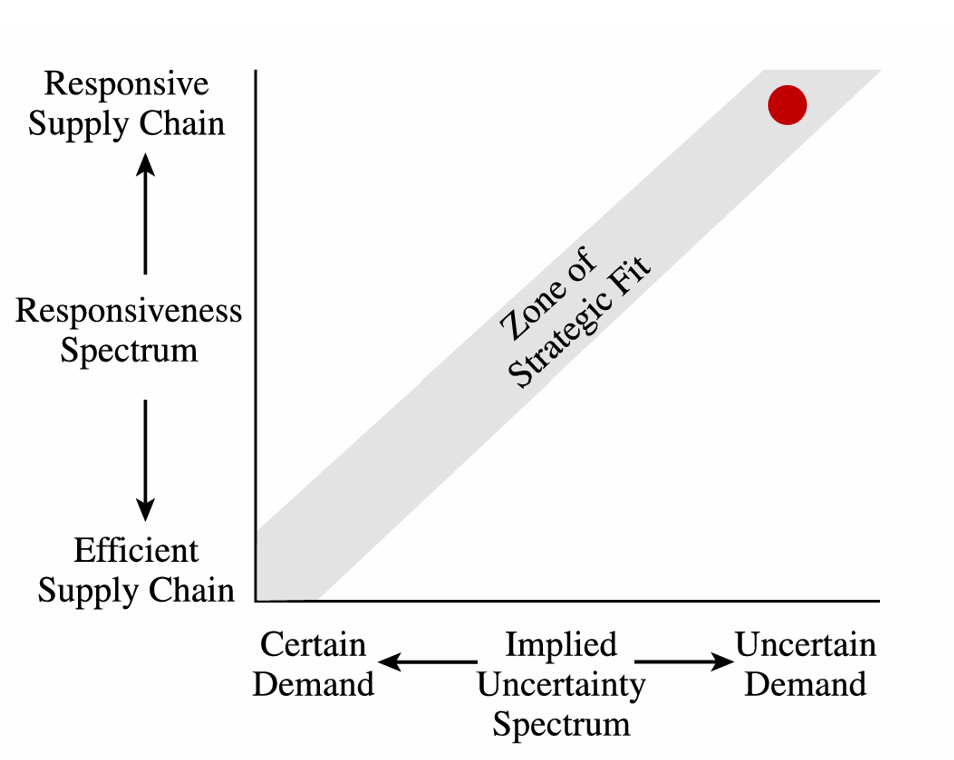
\includegraphics[width=0.95\linewidth]{Responsiveness-uncertainty_spectrum.png}
        \caption{Responsiveness-uncertainty spectrum\cite{responsiveness-uncertainty}} %最好也cite一下这个图的来源
    \end{subfigure}
    \hfill
    \begin{subfigure}{0.48\textwidth}
        \centering
        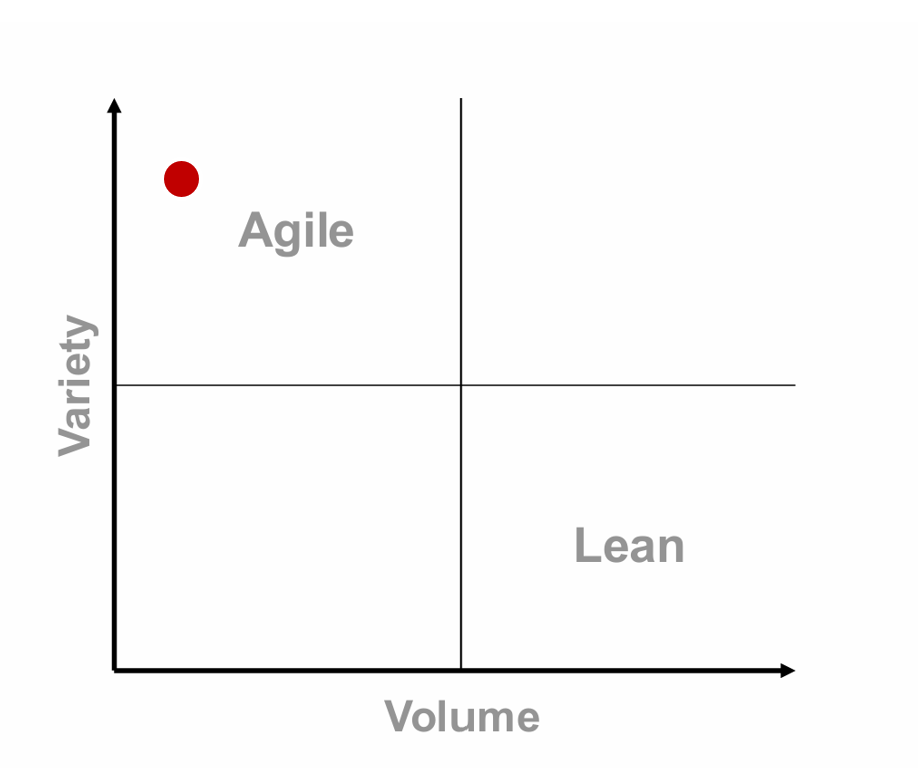
\includegraphics[width=0.95\linewidth]{Fisher_variety-volume_supply_chain_model.png}
        \caption{Fisher variety-volume supply chain model\cite{fisher} }
    \end{subfigure}

    \caption{Operating strategy positioning of the system within the responsiveness--uncertainty spectrum and Fisher variety--volume framework. The red markers indicate the operational characteristics of the rabbit vehicle testing system.}

    \label{fig:lean_vs_agile}
\end{figure}

\subsection{Flow Strategy (Push vs Pull)}

At the same time, the system exhibits a mixed push--pull strategy rather than relying entirely on either approach. Push-based processes are initiated in anticipation of operational demand and typically rely on advance preparation and inventory positioning. This improves responsiveness and reduces recovery delay for critical components, particularly where supplier lead times or disruption consequences are significant. In contrast, pull-based processes are triggered reactively by actual operational demand or failure events, reducing unnecessary inventory and improving resource efficiency where immediate availability is less critical.

In this system, different components exhibit substantially different operational characteristics, supplier dependencies, and disruption impacts. As a result, the push--pull boundary cannot be defined uniformly across the entire system but must instead vary depending on the risk profile and recovery requirements of individual components. Components associated with higher disruption impact or longer recovery duration are managed using more push-oriented preparation, whereas lower-risk components can be managed more reactively through pull-based replenishment.

This differentiated approach allows the system to balance responsiveness and inventory efficiency by directing preparatory resources towards operationally critical components, and constitutes a combined push–pull flow strategy in which the push–pull boundary varies across components rather than being defined uniformly. The component-level risk classification developed in Section~\ref{sec:risk_classification} determines where this boundary is drawn for each component, and directly informs the differentiated inventory management strategy presented in Section~\ref{sec:inventory_management}.

\subsection{Conclusion}

Overall, the supply chain can be characterised as a centralised, agile, and failure-driven system, where decisions are adapted to uncertainties associated with different components. And the strategy reflects a strong alignment between system requirements and supply chain design, ensuring that operational continuity is maintained under uncertain conditions.

\section{Supply Chain Planning}
\label{sec:supply_chain_planning}

\subsection{Planning Framework}%**
\label{subsec:supply_chain_planning_framework}

Given the operational nature of the system, supply chain planning is driven by the objective of maximising system availability through effective management of failure risk.

Thus, the key consideration is how different failures affect the continuity of testing, particularly in terms of how likely they are to occur and how long recovery takes following disruption. Since even relatively minor component failures can prevent safe system operation, most components are treated as operationally critical within the testing cycle. For example, both a major motor failure and the loss of a small wheel fastener may render the vehicle unavailable for testing despite their very different physical scale and cost.

As a result, planning decisions focus primarily on failure likelihood and recovery duration; these factors together determine the level of inventory preparation and supply responsiveness required across different components.

\subsection{Failure Mode and Effect Analysis (FEMA)}

To support the planning framework, a structured failure analysis is carried out using a simplified Failure Mode and Effects Analysis (FMEA)\cite{FMEA_lecture_notes}\cite{fmea_supplychain}.

Failure likelihoods are estimated using a combination of available engineering information, including component specifications, expected lifetime data, operating limits, and engineering judgment obtained through consultation with FSUK team members. In particular, impact-related failures are assessed based on the physical characteristics of each component qualitatively, including impact exposure, structural protection, and expected mechanical loading during testing activities. As operational data becomes available through testing, these estimates can be refined to improve the accuracy of subsequent simulation and inventory planning.

The resulting failure probabilities are then used to support subsequent operational simulation and inventory planning analysis. Since consistent quantitative data is not available across all components and operating conditions, the FMEA is applied in a qualitative and semi-quantitative manner, focusing on relative differences between components rather than precise numerical prediction.

A summary of the FMEA results for the powertrain components is presented in Table~\ref{tab:fmea} as a representative example, and the same framework is applied across all other subsystems.

\begin{table}[H]
\centering
\small
\renewcommand{\arraystretch}{1}

\caption{Failure Mode and Effect Analysis for Powertrain Components}
\label{tab:fmea}

\begin{tabularx}{\textwidth}{
l
X
p{0.14\textwidth}
X
p{0.12\textwidth}
}
\toprule

Component &
Non-collision Failure Mode &
Non-collision Failure Prob. &
Collision Failure Mode &
Collision Failure Prob. \\

\midrule

Electric Motor &
Overheating / Bearing wear &
0.0002 &
Impact-induced damage (minor) &
0.005 \\

Controller (VCU) &
Overcurrent / Firmware fault &
0.0003 &
Shock / Connection fault &
0.008 \\

Inverter &
Overheating / IGBT failure &
0.0003 &
Impact-induced electrical fault &
0.010 \\

Drive Shaft &
Wear / Fatigue &
0.0005 &
Impact bending &
0.080 \\

Sprocket &
Wear &
0.0005 &
Impact break &
0.100 \\

Chain &
Fatigue / Elongation &
0.0010 &
Impact failure &
0.100 \\

Differential &
Gear / Bearing wear &
0.0005 &
Impact-induced internal damage &
0.010 \\

Power Wiring &
Loose / Connector failure &
0.0020 &
Impact disconnection &
0.050 \\

\bottomrule
\end{tabularx}
\end{table}

The results confirm that collision-induced failure probabilities are consistently one to two orders of magnitude greater than non-collision probabilities across all powertrain components, justifying the supply chain's primary focus on collision recovery over non-collision failure management.

\subsection{Operational Simulation - Monte Carlo}

While the FMEA provides detailed information on failure behaviour, supply chain planning additionally requires an understanding of how different components influence spare consumption and recovery responsiveness across the system.

To support this, a simplified operational Monte Carlo simulation is introduced using the failure probabilities and lead times obtained from the FMEA\cite{montecarlo}. Each simulation run represents a typical operational quarter consisting of 75 contact events, estimated from the financial and market growth analysis conducted by Harry. Contact events include both minor and major impacts occurring during testing activities. Component failures during each quarter are then estimated using a binomial distribution based on the corresponding failure probabilities obtained from the FMEA. And to reduce stochastic variation and improve the stability of the results, the simulation is repeated over 1000 Monte Carlo iterations.
\[
N_{\text{failure}} \sim \text{Binomial}(75,\, P_{\text{failure} \mid \text{contact}})
\]

\begin{table}[h]
\centering
\caption{Monte Carlo-based spare planning results for powertrain components over a typical operational quarter.}
\label{tab:inventory_policy}
\renewcommand{\arraystretch}{1.3}

\resizebox{\textwidth}{!}{
\begin{tabular}{lccccc}
\hline

\textbf{Part} &

\makecell{\textbf{Lead Time} \\
\textbf{(days)}} &

\makecell{\textbf{Failure Prob.} \\
\textbf{per Contact}} &

\makecell{\textbf{Average Spare} \\
\textbf{Consumption} \\
\textbf{(/quarter)}} &

\makecell{\textbf{Expected Consumption} \\
\textbf{During Lead Time}} &

\makecell{\textbf{Recommended} \\
\textbf{Spare Inventory}} \\

\hline

Electric Motor & 35 & 0.005 & 0.37 & 0.15 & 1 \\
Controller (VCU) & 7 & 0.008 & 0.59 & 0.05 & 1 \\
Inverter & 28 & 0.010 & 0.77 & 0.24 & 1 \\
Drive Shaft & 21 & 0.080 & 5.95 & 1.37 & 2 \\
Sprocket & 14 & 0.100 & 7.50 & 1.16 & 2 \\
Chain & 7 & 0.100 & 7.39 & 0.57 & 1 \\
Differential & 14 & 0.010 & 0.76 & 0.12 & 1 \\
Power Wiring & 3 & 0.050 & 3.89 & 0.13 & 1 \\

\hline
\end{tabular}
}

\end{table}

\subsection{Inventory Policy}

The simulation results provide an estimate of the expected component consumption occurring during supplier lead time, representing the expected spare demand before replenishment can be completed.

Inventory requirements are determined using a conservative availability-oriented policy: expected consumption values are rounded upwards, providing redundancy against non-collision failures and peak demand variability. And a minimum of one spare is maintained for all components regardless of failure frequency, given that long lead times and operational criticality make fully reactive replacement impractical.

\subsection{Risk Classification}
\label{sec:risk_classification}

Building on the inventory policy analysis, a replenishment classification framework is introduced to distinguish different spare preparation and supply response behaviours across the system.

As illustrated in Figure~\ref{fig:riskclassification1}, components are classified according to two key dimensions: expected spare parts consumption and supplier lead time. Expected spare parts consumption reflects the inventory burden associated with each component, while lead time represents the level of supply responsiveness required for recovery.

Fixed operational boundaries are used to define the classification regions, where components with expected spare parts consumption greater than two units per quarter are classified as high-consumption components, while components with lead times exceeding two weeks are classified as high-responsiveness components.

\begin{figure}
    \centering
    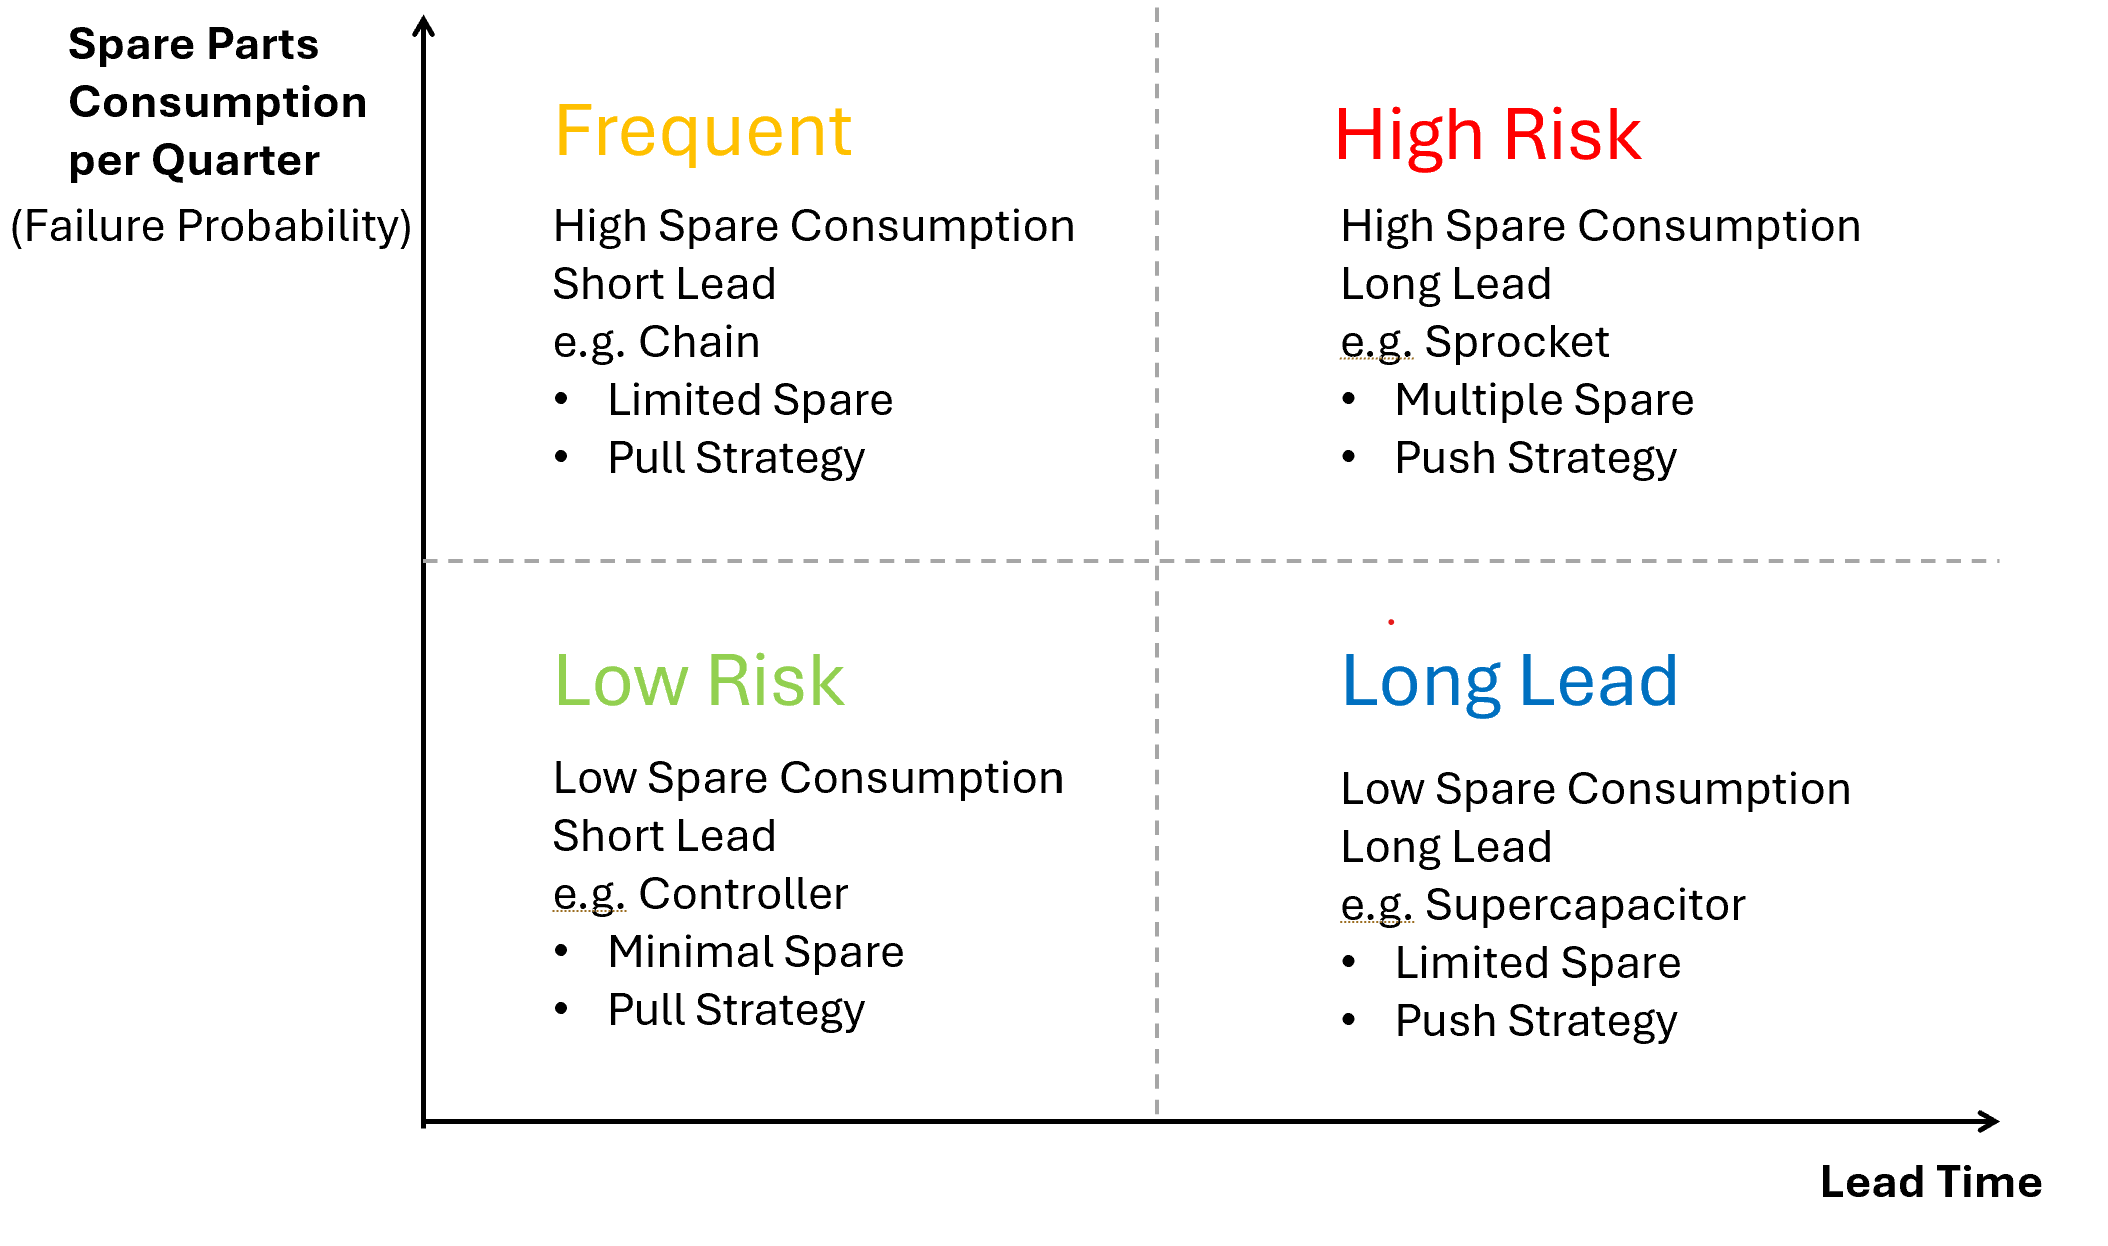
\includegraphics[width=0.65\linewidth]{Classification_of_component_risk.png}
    \caption{Conceptual classification of component risk}
    \label{fig:riskclassification1}
\end{figure}

Based on this, components are classified according to two key factors: failure likelihood and lead time, which together determine how frequently disruptions occur and how long the system is affected when they do. A conceptual classification is first introduced in Figure~\ref{fig:riskclassification}, defining four categories based on these dimensions. The boundaries between categories are defined using median values, providing a consistent and relative basis for comparison.

The framework is then evaluated under contact operating conditions, as shown in Figure~\ref{fig:collision}. Under these conditions, several driveline components shift towards regions requiring higher inventory levels and more responsive supply chain strategies.

From this classification, components can be grouped into four replenishment categories: high-risk components requiring both high inventory preparation and responsive supply; frequent-consumption components requiring continuous replenishment; strategic spare components with low expected consumption but long replenishment delay; and low-risk components that can be managed more reactively.

\begin{figure}
    \centering
    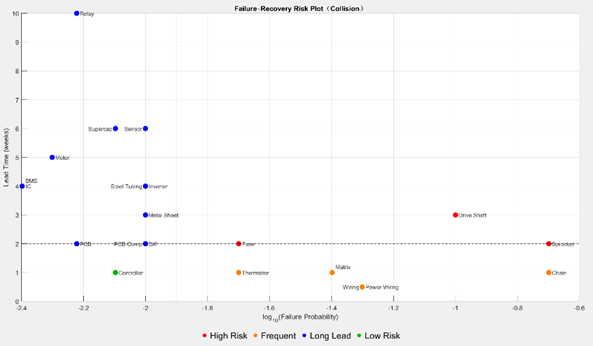
\includegraphics[width=0.85\linewidth]{collision.png}
    \caption{Component classification under collision conditions (need further updates after getting data from other teams mates and make the text in the figure bigger)}
    \label{fig:collision}
\end{figure}
%need update from Michael

\subsection{Inventory management}
\label{sec:inventory_management}

Based on the replenishment classification framework, inventory management is differentiated across components rather than applying a uniform spare policy throughout the system. As illustrated in Figure~\ref{fig:riskclassification1}, different combinations of spare consumption behaviour and lead time require different replenishment strategies in order to balance operational continuity with inventory efficiency.

High-risk components, such as Sprocket, are managed using strongly push-oriented inventory preparation. Multiple spare units are pre-positioned before operation in order to minimise disruption during testing activities, as reactive replenishment would be unable to respond sufficiently quickly under these conditions.

In contrast, Frequent components, such as Chain, are managed using a hybrid replenishment approach. Limited local inventory is maintained to support immediate replacement, while replenishment is triggered continuously during operation. This allows inventory levels to remain responsive to actual operational demand without requiring excessive stock holding.

Long lead components, such as Supercapacitor, are managed as strategic standby inventory. Although failures occur infrequently, at least one spare unit is retained due to the operational impact associated with delayed replenishment.

Finally, low-risk components, such as the controller, are managed more reactively through pull-oriented replenishment, where replacement is largely triggered by operational demand rather than advance preparation.

Overall, the inventory management strategy reflects a differentiated push--pull structure in which replenishment behaviour is adapted according to the operational characteristics of different components.

\subsection{Risk Mitigation}

While the inventory management strategy improves operational availability through spare preparation, additional mitigation measures are introduced to reduce dependence on inventory alone. These measures focus on reducing either replenishment burden or supply responsiveness requirements across different component categories.

For high-risk and long-lead components, mitigation primarily focuses on reducing supply vulnerability through supplier diversification, component standardisation, and the identification of compatible substitute parts. These measures reduce dependence on individual suppliers and improve recovery flexibility under disruption conditions.

For components associated with frequent spare consumption, mitigation focuses on reducing operational wear and simplifying replacement procedures. Improvements in durability, modularity, and ease of maintenance help reduce spare consumption rates while enabling faster operational recovery during testing activities.

In contrast, mitigation measures for low-risk components remain relatively limited, as the operational benefit of further intervention is unlikely to justify the associated increase in complexity and cost.

\subsection{Conclusion}

The planning analysis shows that component prioritisation can be based on failure likelihood and disruption duration. By combining FMEA with operational Monte Carlo simulation and risk classification, components are grouped according to their expected inventory demand and supply response characteristics. This provides a structured basis for defining inventory policies, inventory management, and risk mitigation across the system.

\section{Supply Chain Operation}

\subsection{Operational Flow}

\begin{figure}
    \centering
    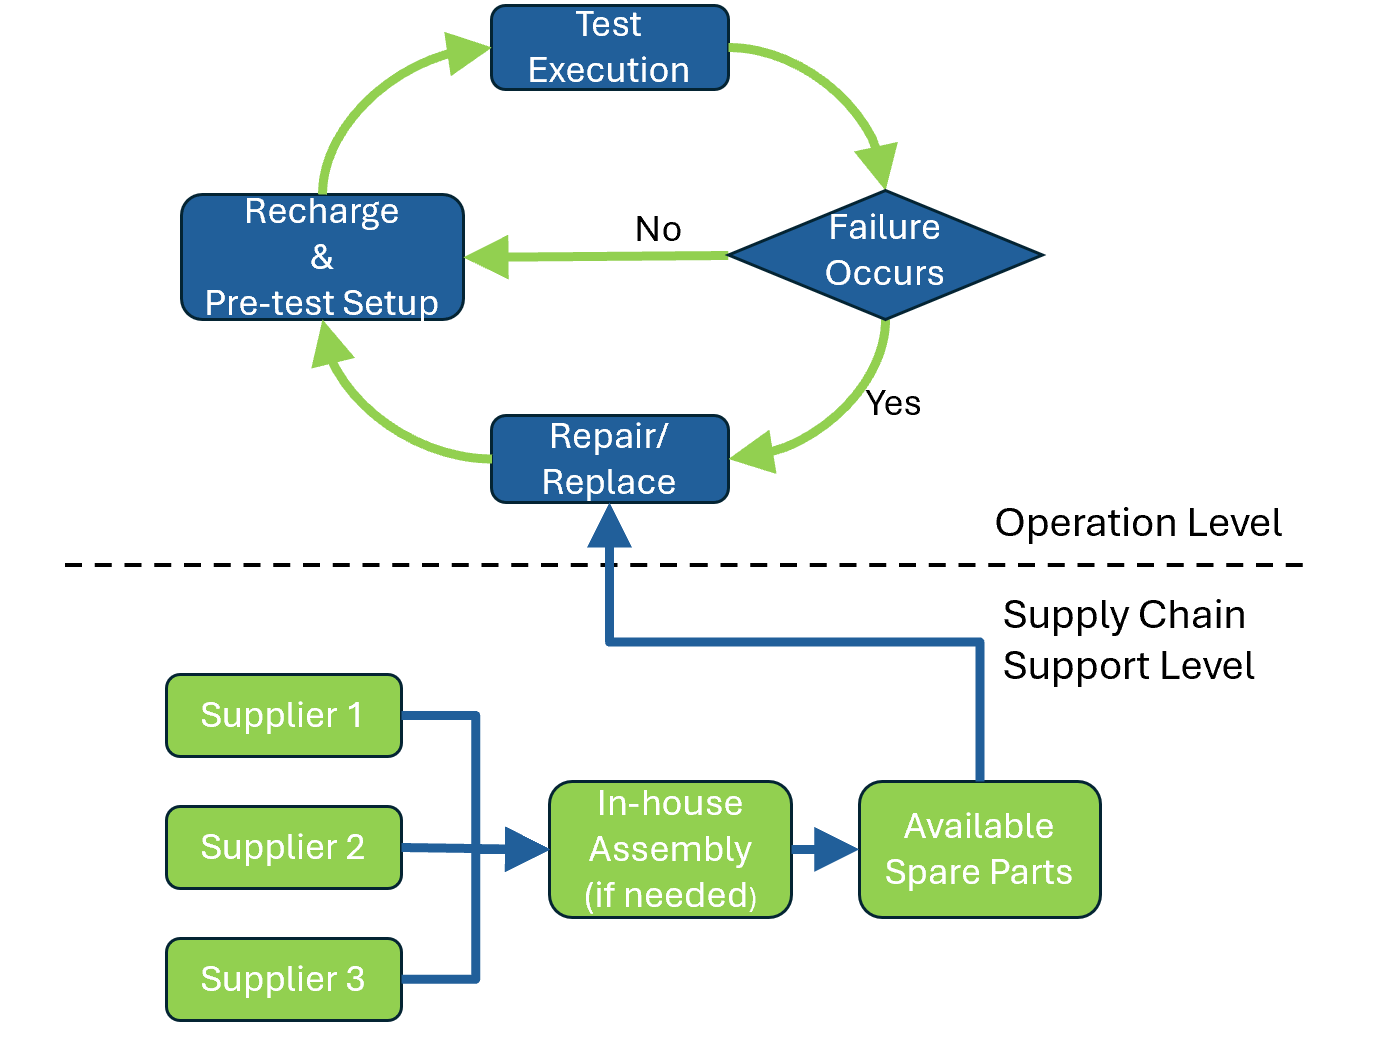
\includegraphics[width=0.5\linewidth]{operation1.png}
    \caption{Operational cycle and supply chain support structure}
    \label{fig:operation}
\end{figure}

The operation of the system is illustrated in Figure~\ref{fig:operation}. The system operates as a closed loop, in which the vehicle is repeatedly used for testing rather than following a linear production process.

Each cycle consists of a preparation stage, including recharge and pre-test setup, followed by test execution. After each test, a decision point determines whether a failure has occurred. If no failure is detected, the system proceeds directly to the next cycle; otherwise, it transitions to repair or replacement before returning to operation.

This operational loop is supported by a supply chain layer, which ensures that spare parts are available when needed, enabling the system to recover and continue testing.

\subsection{Process Behaviour}

The operational cycle described in Figure~\ref{fig:operation} exhibits different characteristics across its stages and therefore cannot be represented by a single process model.

The preparation and test execution stages are highly structured and repeatable, with clearly defined procedures and consistent execution. These stages resemble lean operation, where efficiency and standardisation are prioritised due to the repetitive nature of the process.

In contrast, the recovery stage following a failure is inherently less predictable. The type and extent of damage can vary significantly, particularly under collision conditions, requiring flexible responses and case-by-case decision-making. This stage therefore exhibits characteristics of agile operation, where responsiveness and adaptability are prioritised over efficiency.

As a result, the system combines both lean and agile behaviours within the same operational cycle, with the dominant mode depending on the stage of operation.

\subsection{Downtime and Performance Constraints}

The performance of the system is primarily constrained by non-execution time, as any delay outside the test execution phase directly reduces testing throughput. A summary of the operational time distribution is presented in Table~\ref{tab:operation_time}.

\begin{table}[H]
\centering
\small
\renewcommand{\arraystretch}{1}

\caption{Summary of Operational Time Distribution}
\label{tab:operation_time}

\begin{tabularx}{\textwidth}{l X c c}
\toprule
Stage & Description & Time & Role in Process \\
\midrule
Recharge & Battery charging & $\sim$10 s & Non-value-added \\
Pre-test Setup & System checks and preparation & $\sim$430 s & Non-value-added \\
Test Execution & Dynamic crossing test & $\sim$36 s & Value-added \\
Recovery & Repair/replacement & 10 min--2 days & Non-value-added \\
\bottomrule
\end{tabularx}
\end{table}

Following the lean distinction between value-added and non-value-added activities, test execution represents the primary value-added stage as it directly contributes to the generation of testing data. In contrast, recharge, setup, and recovery activities increase operational cycle time without directly contributing to testing output.\cite{value_added}

As shown in Table~\ref{tab:operation_time}, the pre-test setup stage accounts for a significantly larger portion of the cycle compared to the execution phase. This indicates that system throughput is not limited by the test itself, but by the activities required before and after each run. In addition, the recovery stage introduces substantial variability, ranging from short repairs to extended structural recovery, further increasing uncertainty in overall cycle time.

As a result, system performance is strongly influenced by preparation efficiency and recovery responsiveness rather than execution speed alone.

\subsection{Process Improvements}

The previous analysis shows that operational performance is influenced primarily by preparation efficiency and recovery responsiveness. As a result, process improvements focus on reducing non-value-added activities and minimising disruption throughout the operational cycle.

For preparation activities, improvements are achieved mainly through process standardisation, workspace organisation, and more efficient task sequencing. Since these stages are repetitive and relatively predictable, lean operational principles can be applied to reduce unnecessary delay before each testing cycle and improve overall operational throughput.

In contrast, recovery activities require a more responsive approach due to the variability associated with component failures and operational disruption. Under these conditions, rapid replacement and recovery become more important than process efficiency alone, making recovery responsiveness a key operational consideration within the system.

One important extension of this recovery approach is the introduction of a modular recovery structure through the use of prepared standby resources. Rather than performing repair activities directly within the operational cycle, replacement units can be deployed immediately following operational failure, allowing testing activities to continue while repair and maintenance are carried out separately \cite {modular}.

This effectively transforms recovery from a sequential process into a parallel operational structure, reducing the propagation of downtime across the testing cycle and significantly improving operational responsiveness. Instead of waiting for repair to be completed before operation resumes, replacement and recovery can occur simultaneously, minimising disruption during testing activities.

Importantly, from a supply chain perspective, this modular strategy does not necessarily increase overall inventory requirements. As established previously, the system already maintains at least one spare unit for all components due to its availability-oriented planning strategy. The modular recovery structure, therefore, reorganises existing spare capability rather than duplicating the entire system.

In addition, the concept is not limited to full vehicle replacement. At the chassis level, a prepared spare shell can be maintained as a modular replacement unit, allowing the structural assembly to be swapped immediately after a collision, while the damaged shell undergoes repair separately. Similar principles can also be applied to other components, such as wired supercapacitor assemblies or replacement electrical units, which can be pre-prepared and swapped rapidly during operation. This further reduces recovery delay while improving flexibility within the operational cycle.

Following recovery, repaired systems or modules are returned to standby status and reintegrated into the active spare pool, forming a closed refurbishment loop in which recovered assets continuously rotate back into operational readiness. This ensures that spare capability is maintained dynamically rather than depleted over time.

\subsection{Key Activities}

While the previous sections describe the operational structure of the system, five ongoing activities are required to maintain operational continuity during testing.

\paragraph{Inventory Coordination}
Inventory Coordination monitors component stock levels against the reorder thresholds established in the planning analysis. For high-risk and frequent-consumption components such as sprockets and chains, stock levels are checked after each testing session, and replenishment is triggered immediately when inventory falls below the recommended spare level. For long-lead components, replenishment is initiated in advance of anticipated demand rather than reactively, given that supplier lead times may extend to several weeks.

\paragraph{Post-Collision Inspection}
Post-Collision Inspection is initiated immediately following any contact event. Each affected subsystem is assessed against a standard checklist to determine whether components require replacement or can remain in service. Driveline components including drive shafts, sprockets, and chains are prioritised given their elevated collision failure probabilities identified in the FMEA. A replacement decision is made on-site, and the relevant spare is drawn from the pre-positioned inventory pool before the next test cycle begins.

\paragraph{Spare Rotation and Refurbishment}
Spare Rotation and Refurbishment builds on the modular recovery structure established in Section 9.4.4, ensuring that recovered components are systematically returned to the active spare pool. Following each replacement, damaged components are assessed for repairability against a standard serviceability criterion. Those cleared for reuse are refurbished and reintegrated as standby spares, maintaining spare pool depth without requiring continuous new procurement. This approach is aligned with circular economy principles, and is particularly important for high-cost, long-lead components such as motors and inverters, where repeated replacement from external suppliers would be both costly and operationally disruptive.

\paragraph{Supplier Management}
Supplier Management focuses on maintaining replenishment flexibility during operation. For critical components, at least two qualified suppliers are identified in advance to reduce exposure to single-source disruption. Urgent procurement procedures are established for high-risk components, with agreed lead time expectations documented per supplier. Compatibility across suppliers is verified during the planning stage to ensure that substitute components can be deployed without modification.

\paragraph{Data Refinement}
Data Refinement is conducted at the end of each operational quarter. Actual failure counts and recovery durations recorded during testing are compared against the FMEA estimates and Monte Carlo predictions. Where significant deviations are observed, failure probabilities are updated and the simulation is rerun to recalibrate spare inventory levels and replenishment thresholds for the following quarter. This ensures that supply chain parameters evolve with operational experience rather than remaining fixed at initial estimates.

\subsection{Conclusion}

The operational structure of the system is defined by a closed recovery loop, in which preparation, execution, failure detection, and recovery rotate continuously across each testing session. Within this loop, lean principles govern the preparation and execution stages, while agile responsiveness drives the recovery stage. Process improvements, including modular recovery, further reduce non-value-added time across the cycle. These improvements are sustained in practice through five ongoing key activities. Together, these elements ensure that operational continuity is maintained under uncertain conditions,  and as established in Section 7.3.3, commercial viability depends on sustained utilisation rates and minimal track downtime; the supply chain operations developed here are precisely what deliver this in practice.

\section{Conclusion}

The supply chain for the rabbit vehicle is driven by the need to maintain continuous operation under uncertainty. Through failure analysis, Monte Carlo simulation, and risk classification, components are prioritised by their impact on system continuity, with inventory and mitigation efforts allocated accordingly. Beyond inventory, modular recovery approaches further reduce disruption by decoupling repair activities from the active operational cycle.

Overall, the system can be characterised as a centralised, outsourcing, agile, and failure-driven supply chain. As operational experience accumulates through failure records, recovery data, and client feedback, supply chain parameters can be continuously recalibrated — transforming it from a static design into a learning system that grows more resilient over time. Ultimately, a supply chain designed around availability and rapid recovery directly translates into service reliability — which, for an early-stage TaaS company, is the product being sold.

\section*{Appendix: Data Sources and Contributions}

The data used in the FMEA and the subsequent analysis are derived from the engineering design of the project. Data for the different subsystems were provided by team members responsible for their respective designs:

\begin{itemize}
    \item Chassis: Toby McConnell (Section 1)
    \item Wheels: Ziyang Xing (Section 2)    
    \item Powertrain: Yuze Jiang (Section 3)
    \item Battery: Paul Vogelburg (Section 4)
\end{itemize}

Where applicable, detailed and publicly available data sources are cited in the corresponding sections of the main text.

\compactbib
% --- END INLINE: Yuze Jiang/Business/EEM.tex ---
\end{refsection}

% Harry's Business chapter uses helper environments from this file
% (tightitemize, tightenumerate). Loaded only just before his refsection.
% --- BEGIN INLINE: HarryEmes/Business/harry_business_macros.tex ---
% Helper environments for Harry's business chapter (tight lists).
% In the merged build the chapter formatting matches every other chapter
% (no compact-heading override), per the user's "same numbering style"
% requirement. The original compact-chapter override is intentionally
% omitted here.

\newenvironment{tightitemize}%
  {\begin{itemize}\setlength{\itemsep}{2pt}\setlength{\parskip}{0pt}\setlength{\topsep}{4pt}}%
  {\end{itemize}}
\newenvironment{tightenumerate}%
  {\begin{enumerate}\setlength{\itemsep}{2pt}\setlength{\parskip}{0pt}\setlength{\topsep}{4pt}}%
  {\end{enumerate}}
% --- END INLINE: HarryEmes/Business/harry_business_macros.tex ---

\begin{refsection}
\graphicspath{{../HarryEmes/Business/figures/}{../HarryEmes/Business/}}
% --- BEGIN INLINE: HarryEmes/Business/harry_business_body.tex ---
% =====================================================================
\chapterauthor{Financial Analysis}{Harry Emes}
% =====================================================================

\noindent This chapter discusses the five-year TaaS plan using a
Python model linking
capex, opex, and revenue; P\&L and free cash flow; break-even and one-at-a-time
sensitivities (Sections~\ref{sec:breakeven}--\ref{sec:business_sensitivity});
NPV/IRR (Section~\ref{sec:npv}); and downtime stress
(Section~\ref{sec:downtime}). Market sizing and day-rate values follow
Section~\ref{sec:market_and_competition}. Fleet-recovery and our growth rate assumptions align with the
preceding business chapters.

\medskip

\noindent \textbf{Headline financial evaluation}:

\begin{tightitemize}
  \item \textbf{CAPEX commitment:} \totalCapex over five years
        (\capexPerVehicle per vehicle $\times$ 3 vehicles +
        \pounds50\,k Y1 setup). Cumulative revenue first exceeds
        cumulative CAPEX in \inversionCrossover.
  \item \textbf{Five-year trajectory:} \yOneRevenue revenue $\to$
        \yFiveRevenue; break-even in \breakEvenYear at
        \breakEvenDays test days/year (contribution
        \contributionMargin per day).
  \item \textbf{Funding:} \seedRound seed + \seriesARound Series~A,
        total \totalRaise equity. Peak cumulative cash outflow
        occurs end-Y2 ($\sim$\pounds90\,k minimum cash left).
  \item \textbf{Capital return:} project NPV \npvBase at a 20\% VC
        discount rate, \npvHurdle at a 25\% hurdle rate, IRR \irr,
        all including a \terminalValue terminal value at $2.5\times$
        Y5 revenue.
  \item \textbf{Sensitivity:} day-rate and utilisation dominate; a
        $\pm 20\%$ swing in either drives $\sim$\pounds 270--370\,k
        in Y3 EBIT.
  \item \textbf{Downtime sensitivity:} NPV stays positive through
        \downtimeBreak unplanned fleet downtime, but Y5~EBIT turns
        negative once downtime exceeds $\sim$20\%. Fleet maintenance
        is therefore the most vital execution
        dependency on the financial plan.
\end{tightitemize}

\noindent \textbf{Conclusion}: the TaaS financial structure clears
standard venture-capital thresholds and is
robust to swings in the key parameters with plans made to mitigate the negative affects of the largest factors.
(Section~\ref{sec:business_sensitivity}).

% =====================================================================
\section{Key driver assumptions and their justification}
\label{ch:intro}
\label{sec:why_taas}
\label{sec:assumptions}
% =====================================================================

All headline figures come from one set of python parameters; this section details the major assumptions and justifications for the main inputs into the model.

\paragraph{CAPEX and revenue drivers.} Per-vehicle build of
\capexPerVehicle{} consists of 5 key factors (vehicle \pounds180\,k,
instrumentation \pounds60\,k, safety element additions \pounds25\,k, trailer
\pounds30\,k, spares \pounds15\,k), aligned with the engineering
Bill of Materials~\cite{mcconnell_engineering,xing_engineering,jiang_engineering,vogelberg_engineering}; Y1
\pounds50\,k workshop/data setup sits as a one off cost in year 1. Bronze/Silver/Gold day rates
\pounds6\,k/\pounds8\,k/\pounds10\,k are benchmarked to
AB~Dynamics, UTAC, HORIBA~MIRA, and AVL~\cite{abdynamics_ar2024,utac_facilities,horiba_brake,avl_profile};
tier prices are fixed and the blended rate rises only through
mix-shift (\pounds7.5\,k$\to$\pounds9.5\,k). Billable days per
vehicle 40/70/110/150/220 Y1--Y5 tie to the Market SOM
\cite{mcconnell_business} and reconcile \yFiveRevenue{} to
10--14\% of the \textdollar26\,M SOM (Section~\ref{subsec:som_estimation}).

\paragraph{Opex, variable cost, and tax.} Headcount uses Reed 2025
UK engineering mid-bands~\cite{reed_salaries_2025} with CEO at the
low end of the startup range; gross salaries carry a flat 20\%
additional cost (approx.\ 15\% employer NIC, 3\% auto-enrolment pension,
2\% misc.). Variable cost \pounds2{,}300/day Y1 splits tyres
\pounds800, transport \pounds600 (HMRC 45p/mile on a 200-mile
round trip), crew \pounds400, wear
\pounds500. Fixed opex inflates 3\%/yr from CPIH
\cite{ons_cpi_2025} with slight hiring increases at each vehicle addition. Corporation
tax uses a flat 19\% from Y4~\cite{hmrc_corp_tax} rather than full
banding, consistent with the precision of the revenue forecast.

\paragraph{Capital return.} Discount rate 20\% (VC opportunity cost
\cite{brealey2020}); terminal value at peer-median $2.5\times$ Y5
revenue as in Section~\ref{sec:npv}
\cite{abdynamics_ar2024,damodaran2012,avl_profile}.
Section~\ref{sec:scenarios} stress-tests that terminal-heavy NPV.

% =====================================================================
\section{Cost structure, revenue model and five-year forecast}
\label{ch:cost_revenue}
% =====================================================================

% ---------------------------------------------------------------------
\subsection{CAPEX model: the cost of ownership the operator absorbs}
\label{sec:capex}
% ---------------------------------------------------------------------

Due to the TaaS nature of our business plan, all capital required is
financed from equity until the business turns cash-positive, and is
recovered through the increasing day utilisation. Per-vehicle build is
\capexPerVehicle; the
Y1 setup adds \pounds50\,k in workshop and data-platform
infrastructure setup. Fleet growth (2nd vehicle in Y3, 3rd in Y5) drives
a further \pounds620\,k of capex over Y3--Y5. Total capex over the five-year
plan: \totalCapex.

\begin{figure}[H]
\centering
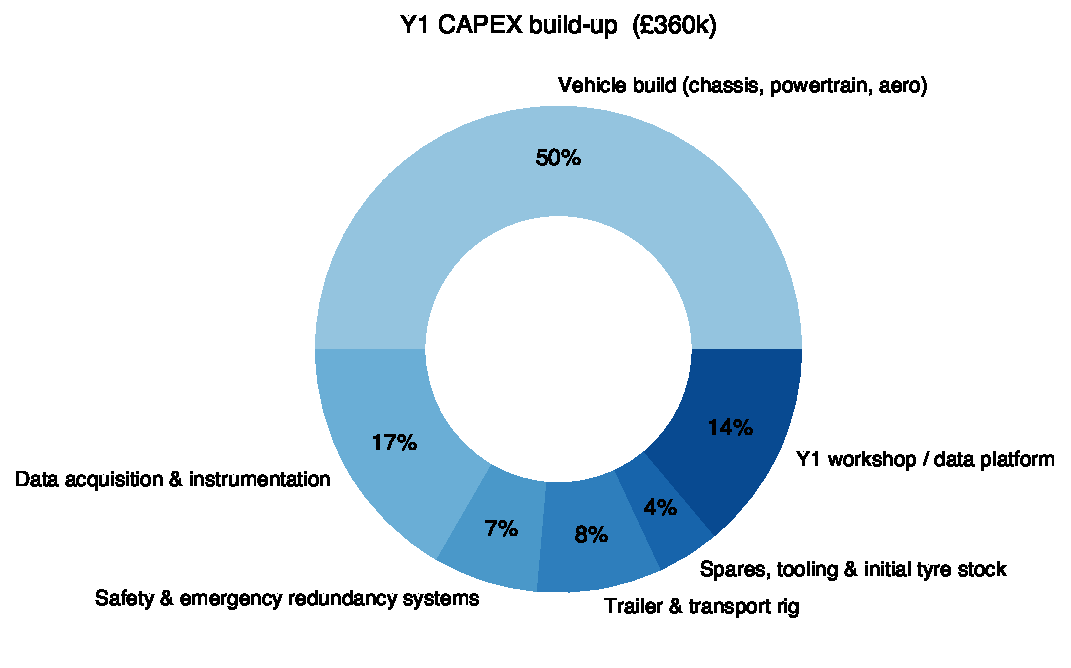
\includegraphics[width=0.92\textwidth,height=0.40\textheight,keepaspectratio]{cost_structure_capex.pdf}
\caption{Y1 CAPEX build-up: per-vehicle line items plus the one-off
  workshop and data-platform setup (same totals as
  Table~\ref{tab:capex_schedule}, Y1 column).}
\label{fig:capex_donut}
\end{figure}

Capital is depreciated on a five-year straight-line basis. No
residual value is modelled at Y5: in a Product-Service-System business, the physical
asset is either refurbished in place following the 9R lifecycle loop (Section~\ref{sec:9r_framework_application})(and therefore stays in service beyond the modelled window) or is
retired in line with industry safety norms.

% --- BEGIN INLINE: HarryEmes/Business/tables/capex_schedule.tex ---
\begin{table}[H]
\centering
\small
\caption{Five-year capex schedule (\pounds k). Per-vehicle build costs 
\pounds310k (component split in Figure~\ref{fig:capex_donut}); 
one-off Y1 company setup \pounds50k.}
\label{tab:capex_schedule}
\begin{tabular}{cccccc}
\toprule
\textbf{Year} & \textbf{New vehicles} & \textbf{Vehicle capex} & \textbf{Other capex} & \textbf{Total} \\
\midrule
1 & 1 & 310 & 50 & \textbf{360} \\
2 & 0 & 0 & 0 & \textbf{0} \\
3 & 1 & 310 & 0 & \textbf{310} \\
4 & 0 & 0 & 0 & \textbf{0} \\
5 & 1 & 310 & 0 & \textbf{310} \\
\bottomrule
\end{tabular}
\end{table}
% --- END INLINE: HarryEmes/Business/tables/capex_schedule.tex ---
% ---------------------------------------------------------------------
\subsection{OPEX model: a fixed-cost-heavy delivery operation}
\label{sec:opex}
% ---------------------------------------------------------------------

\begin{figure}[H]
\centering
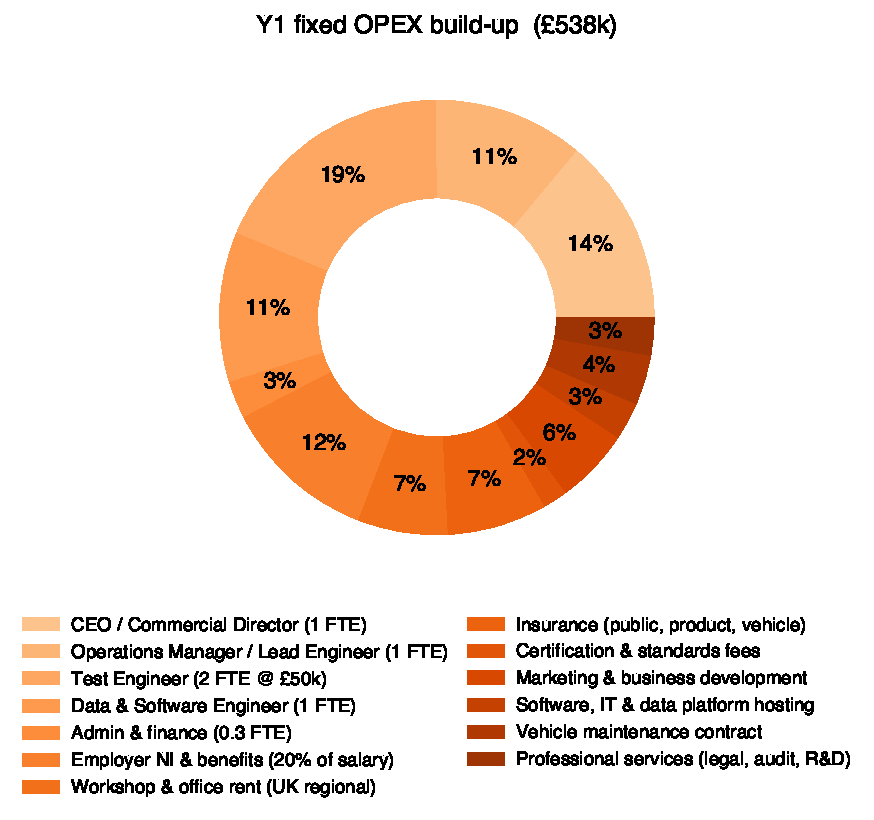
\includegraphics[width=0.92\textwidth,height=0.44\textheight,keepaspectratio]{cost_structure_opex.pdf}
\caption{Y1 fixed-OPEX build-up.}
\label{fig:opex_donut}
\end{figure}

\noindent Fixed opex is dominated by headcount (60\% of the Y1 opex base of
\fixedOpexYOne), with the remainder split across workshop rent,
insurance, certification fees, data-platform hosting, marketing,
vehicle maintenance, and professional services.
The model inflates fixed opex at 3\% per year (UK CPIH 2023--25 trend) and headcount increases by +1 (engineer) then +2 (engineer and PM) with each new vehicle (hiring a PM to account for an increase in operation complexity both present and anticipated).

Variable cost per test day is \pounds2,300 (Y1), comprising tyres
and consumables (\pounds800), transport (\pounds600), crew
travel-and-subsistence (\pounds400), and amortised vehicle wear
(\pounds500). The resulting contribution per test day is
\contributionMargin at a Y2 blended day rate.

% ---------------------------------------------------------------------
\subsection{Revenue model: every pound tethered to fleet utilisation}
\label{sec:revenue}
% ---------------------------------------------------------------------

Revenue is modelled from three key factors: test days
sold, fleet size, and blended day-rate. Day-rate is the
mix-weighted average of the Bronze / Silver / Gold packages
(\pounds6\,k / \pounds8\,k / \pounds10\,k) benchmarked against
the competitor set in Section~\ref{sec:competitive_landscape}
(AB~Dynamics~\cite{abdynamics_ar2024},
UTAC~\cite{utac_facilities},
HORIBA~\cite{horiba_brake}, and AVL~\cite{avl_profile}). Mix-shift
from Bronze-heavy to Gold-heavy over five years drives blended
day-rate from \pounds7.5\,k (Y1) to \pounds9.5\,k (Y5) without
any individual-tier price movement which is important for the pricing
discipline discussed in Section~\ref{sec:business_sensitivity}.

% --- BEGIN INLINE: HarryEmes/Business/tables/revenue.tex ---
\begin{table}[H]
\centering
\small
\caption{Revenue build-up: test days, fleet utilisation, blended day 
rate, and resulting gross-profit stack.}
\label{tab:revenue}
\begin{tabular}{lrrrrr}
\toprule
\textbf{Metric} & \textbf{Y1} & \textbf{Y2} & \textbf{Y3} & \textbf{Y4} & \textbf{Y5} \\
\midrule
Test days sold & 40 & 70 & 110 & 150 & 220 \\
Fleet size & 1 & 1 & 2 & 2 & 3 \\
Utilisation (days/vehicle) & 40 & 70 & 55 & 75 & 73 \\
Blended day rate (\pounds) & 7,500 & 8,000 & 8,500 & 9,000 & 9,500 \\
Revenue (\pounds k) & 300 & 560 & 935 & 1,350 & 2,090 \\
Variable cost (\pounds k) & 92 & 164 & 264 & 368 & 550 \\
Gross profit (\pounds k) & 208 & 396 & 671 & 982 & 1,540 \\
Gross margin (\%) & 69.3 & 70.6 & 71.8 & 72.8 & 73.7 \\
\bottomrule
\end{tabular}
\end{table}
% --- END INLINE: HarryEmes/Business/tables/revenue.tex ---
\paragraph{Reconciliation with market sizing.}
Y5 forecast revenue of \yFiveRevenue ($\approx$\textdollar 2.7\,M)
sits at \mbox{10--14\%} of the serviceable-obtainable-market estimate
(\textdollar 26\,M) in Section~\ref{subsec:som_estimation} -- a
penetration consistent with a credible early-stage entrant.

% ---------------------------------------------------------------------
\subsection{Five-year profit \& loss forecast}
\label{sec:pnl}
% ---------------------------------------------------------------------

Table~\ref{tab:pnl} is the five-year P\&L summary modellby by the results of the cost and revenue models above. Three
features are worth noting:

\begin{tightitemize}
  \item \textbf{EBITDA turns positive in Y4}, well before net
        profit, reflecting the affect of depreciation in a
        capex-heavy service business.
  \item \textbf{Operating-leverage tipping point at Y3.} Gross
        profit grows faster than fixed opex from Y3 onwards;
        Y3 is the \emph{commercial} break-even year, Y4 is the
        \emph{accounting} break-even year.
  \item \textbf{Corporation tax kicks in at Y4}. The Y5 net profit
        of \pounds293\,k is reported after tax.
\end{tightitemize}

% --- BEGIN INLINE: HarryEmes/Business/tables/pnl.tex ---
\begin{table}[H]
\centering
\small
\caption{Five-year P\&L summary (\pounds k). All figures flow from 
the single driver set stated in Sections~\ref{sec:capex}--\ref{sec:revenue}.}
\label{tab:pnl}
\begin{tabular}{lrrrrr}
\toprule
\textbf{Line} & \textbf{Y1} & \textbf{Y2} & \textbf{Y3} & \textbf{Y4} & \textbf{Y5} \\
\midrule
Revenue & 300 & 560 & 935 & 1,350 & 2,090 \\
Variable cost & -92 & -164 & -264 & -368 & -550 \\
Gross profit & 208 & 396 & 671 & 982 & 1,540 \\
Fixed opex & -538 & -616 & -693 & -834 & -983 \\
EBITDA & -330 & -220 & -22 & 149 & 557 \\
Depreciation & -72 & -72 & -134 & -134 & -196 \\
EBIT & -402 & -292 & -156 & 15 & 361 \\
Tax @ 19\% & -0 & -0 & -0 & -3 & -69 \\
Net profit & -402 & -292 & -156 & 12 & 293 \\
\bottomrule
\end{tabular}
\end{table}
% --- END INLINE: HarryEmes/Business/tables/pnl.tex ---
\begin{figure}[H]
\centering
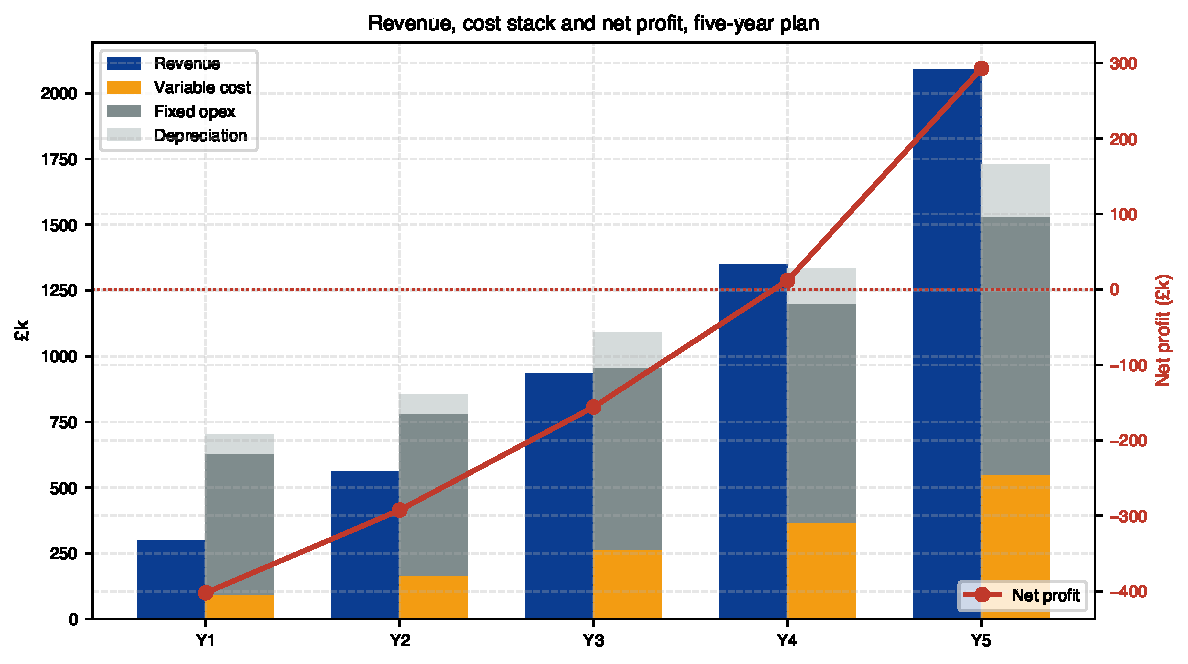
\includegraphics[width=\textwidth]{revenue_ramp.pdf}
\caption{Five-year revenue (blue) against the full cost stack
  (variable, fixed, depreciation) with net-profit trajectory
  overlaid (red, right axis). Net profit crosses zero in Y4 --
  the accounting break-even year -- and reaches \pounds293\,k
  net of tax in Y5.}
\label{fig:revenue_ramp}
\end{figure}

% ---------------------------------------------------------------------
\subsection{Five-year cash-flow forecast}
\label{sec:cash_flow}
% ---------------------------------------------------------------------

A capex-heavy TaaS business requires a great deal of up front cash before being able to become profitable. Figure~\ref{fig:cash} summarises free cash flow,
equity raises, and cumulative cash balance.

\begin{figure}[H]
\centering
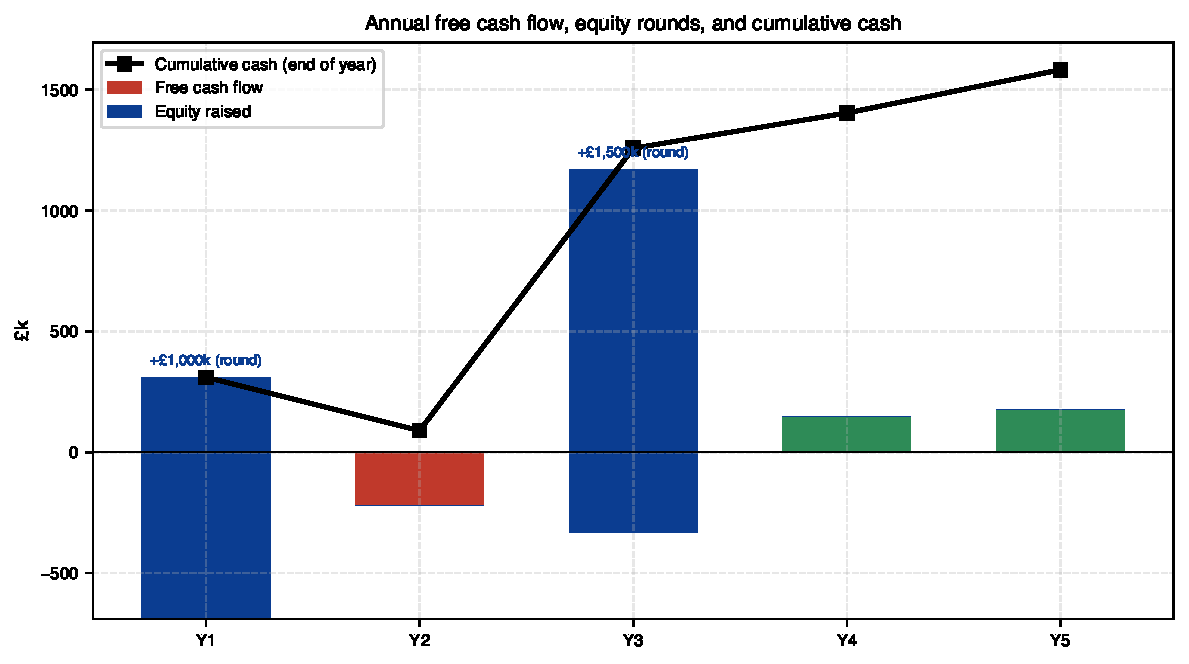
\includegraphics[width=\textwidth]{cash_waterfall.pdf}
\caption{Annual free cash flow (green/red bars), equity rounds
  (blue stacked bars), and cumulative cash balance (black line).
  Cumulative cash reaches its minimum of \pounds90\,k at end-Y2 and turns
  positive from Y3 onwards once the Series~A has closed.}
\label{fig:cash}
\end{figure}

Two moments deserve attention. First, end-Y2 cash balance is
\pounds90\,k which is by far the tightest point in the plan, after absorbing
two years of operating loss. A delayed Series~A would push the
company into a bridge-round conversation; the Series~A
therefore targets a Q4-Y2 close rather than a Y3 close.
Second, Y5 free cash flow is \pounds179\,k positive even after the
\capexPerVehicle third-vehicle purchase proving that our business plan is genuinely
self-funding by Y5.

% =====================================================================
\section{Capital-budgeting assessment}
\label{ch:be_npv}
% =====================================================================

% ---------------------------------------------------------------------
\subsection{Break-even analysis}
\label{sec:breakeven}
% ---------------------------------------------------------------------

Break-even occurs at \breakEvenDays test
days per year. This is the number of days the fleet must sell
annually to cover fixed opex and depreciation:

\begin{equation}
\mathrm{BE_{days}} \;=\; \frac{F + D}{p_{\mathrm{day}} - c_{\mathrm{var}}}
\end{equation}

\noindent where $F$ is annual fixed opex, $D$ annual depreciation,
$p_{\mathrm{day}}$ the Y2 blended day-rate, and $c_{\mathrm{var}}$
the Y2 variable cost per day. The resulting contribution margin
per day is \contributionMargin; fixed costs plus depreciation total
\pounds690\,k~Y2.

\begin{figure}[H]
\centering
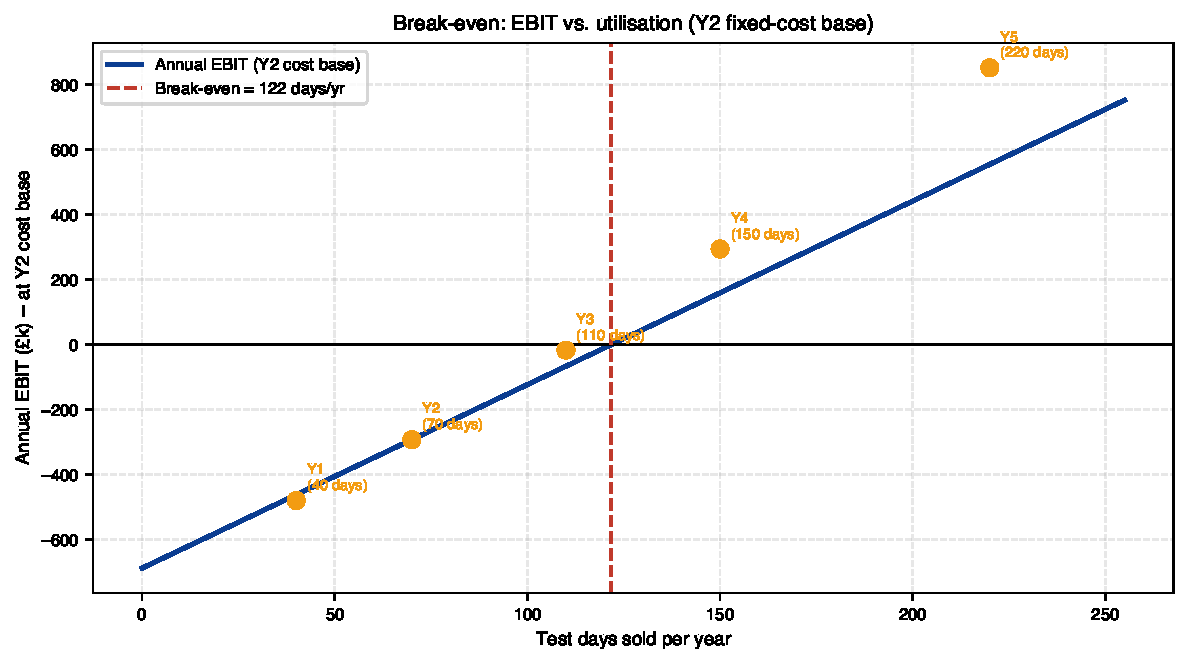
\includegraphics[width=\textwidth]{break_even.pdf}
\caption{Break-even curve: annual EBIT at the Y2 cost base as a
  function of annual test days. The vertical red dashed line marks
  the \breakEvenDays-day break-even point; orange markers show the
  plan's Y1--Y5 planned utilisation trajectory.}
\label{fig:break_even}
\end{figure}

Y1--Y3 sit below break-even (as expected for an early-stage TaaS); Y4 is above; Y5 is comfortably above. Here we see the explicit financial model of the "Taas Burden" in the requirement to keep the business afloat on its road from 40 days to 122 days of utilisation.

% ---------------------------------------------------------------------
\subsection{NPV and IRR -- the capital-budgeting view}
\label{sec:npv}
% ---------------------------------------------------------------------

Because the five-year operational FCFs are loss-making until Y4,
accounting profit is an insufficient test of investability. The
appropriate test is discounted cash flow~\cite{brealey2020}:
can the project, including its terminal value, return more than the
investor's hurdle rate?

\paragraph{Method.} Free cash flows (pre-equity, post-CAPEX) are
the annual series underlying Figure~\ref{fig:cash}. A terminal value is added to
Y5 at the peer-group median EV/Revenue multiple of $2.5\times$
Y5 revenue~\cite{abdynamics_ar2024,damodaran2012}, yielding
\terminalValue. The project NPV at a discount rate $r$ is then

\begin{equation}
\mathrm{NPV}(r) \;=\; \sum_{t=1}^{5} \frac{\mathrm{FCF}_t}{(1 + r)^t} \;+\; \frac{\mathrm{TV}}{(1 + r)^5}.
\end{equation}

\noindent The project IRR is the discount rate at which NPV$=0$.

\paragraph{Result.} Figure~\ref{fig:npv} plots $\mathrm{NPV}(r)$
at representative hurdle rates (same annual FCF series as
Figure~\ref{fig:cash}, pre-equity post-CAPEX, plus the Y5
terminal value stated in the Method paragraph). At the 20\%
VC-central rate the project NPV is \npvBase; at the 25\%
high-hurdle rate it is \npvHurdle; IRR is \irr.

\begin{figure}[H]
\centering
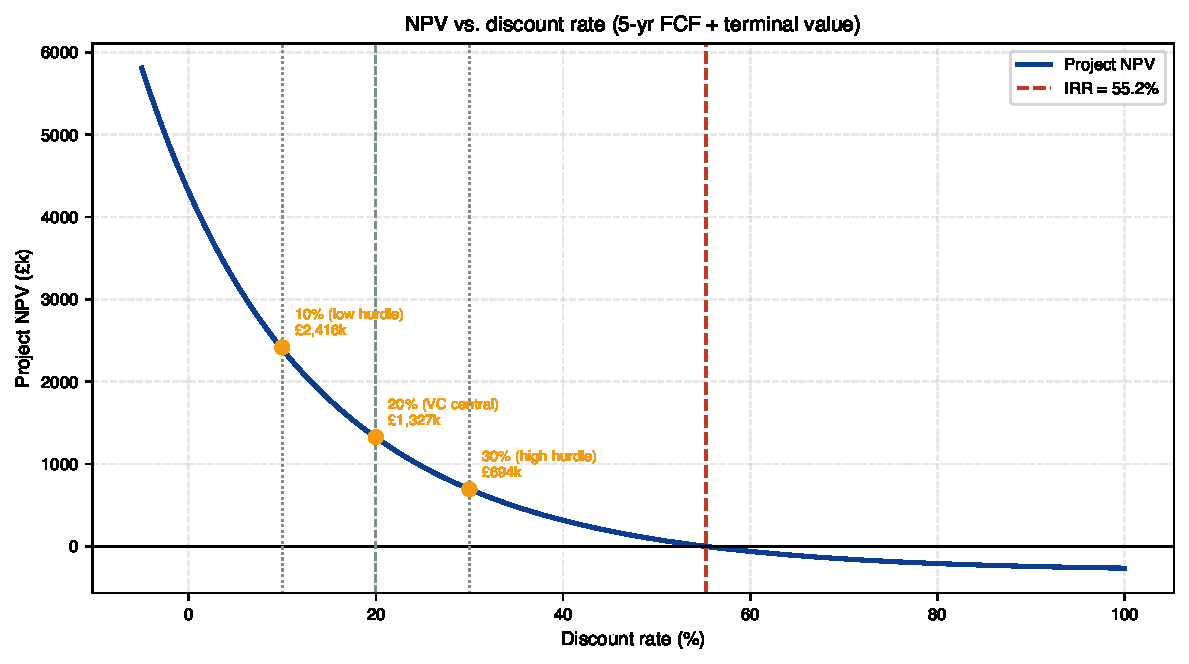
\includegraphics[width=\textwidth]{npv_curve.pdf}
\caption{Project NPV as a function of discount rate $r$. The 10\% /
  20\% / 30\% hurdle points are annotated; the IRR (\irr) is
  marked with the red vertical dashed line.}
\label{fig:npv}
\end{figure}

\paragraph{Interpretation.} The project clears standard VC-hurdle
tests comfortably. Two caveats apply. First, \textbf{almost all
of the NPV is present-value terminal value}, not operational cash
flow: at 20\% the PV of the \terminalValue terminal alone is
\pounds2.1\,M, against \pounds0.8\,M of negative PV from the Y1--Y3
cash outflows. NPV is therefore only as robust as the
exit-multiple assumption. Second, the \irr IRR reflects that a
TaaS project that turns cash-positive in Y5 is, arithmetically, a
very-high-return asset if it can be sold at the terminal multiple;
it does not imply year-by-year operating returns at that level.

% ---------------------------------------------------------------------
\subsection{Sensitivity analysis}
\label{sec:business_sensitivity}
% ---------------------------------------------------------------------

To ensure we survive to realise the Y5 exit value that bolsters our NPV, we performed sensitivity
rankings to determine threats. Each parameter is perturbed by ±20% (±50% for inflation) and the
resulting Y3 EBIT swings ranked in Figure~\ref{fig:business_tornado}.

\begin{figure}[H]
\centering
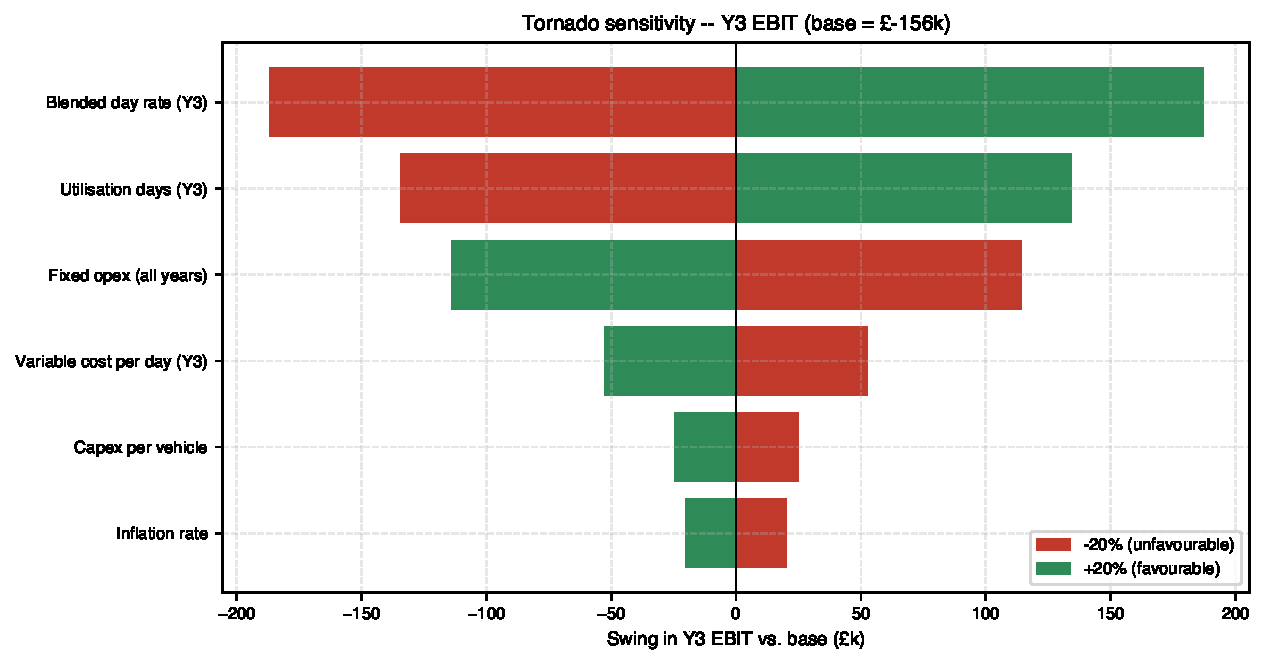
\includegraphics[width=\textwidth]{tornado.pdf}
\caption{Tornado sensitivity of Y3 EBIT to $\pm 20\%$ (or
  $\pm 50\%$) perturbation of each driver.}
\label{fig:business_tornado}
\end{figure}

Two implications follow. First, \textbf{pricing discipline matters
more than cost discipline}: a 20\% day-rate swing is worth
\pounds374\,k of Y3 EBIT whereas a 20\% fixed-opex swing is worth
\pounds228\,k. Second, the two top drivers (day-rate and
utilisation) are the two most directly in the operating team's
control. 

% ---------------------------------------------------------------------
\subsection{Scenario analysis}
\label{sec:scenarios}
% ---------------------------------------------------------------------

\begin{figure}[H]
\centering
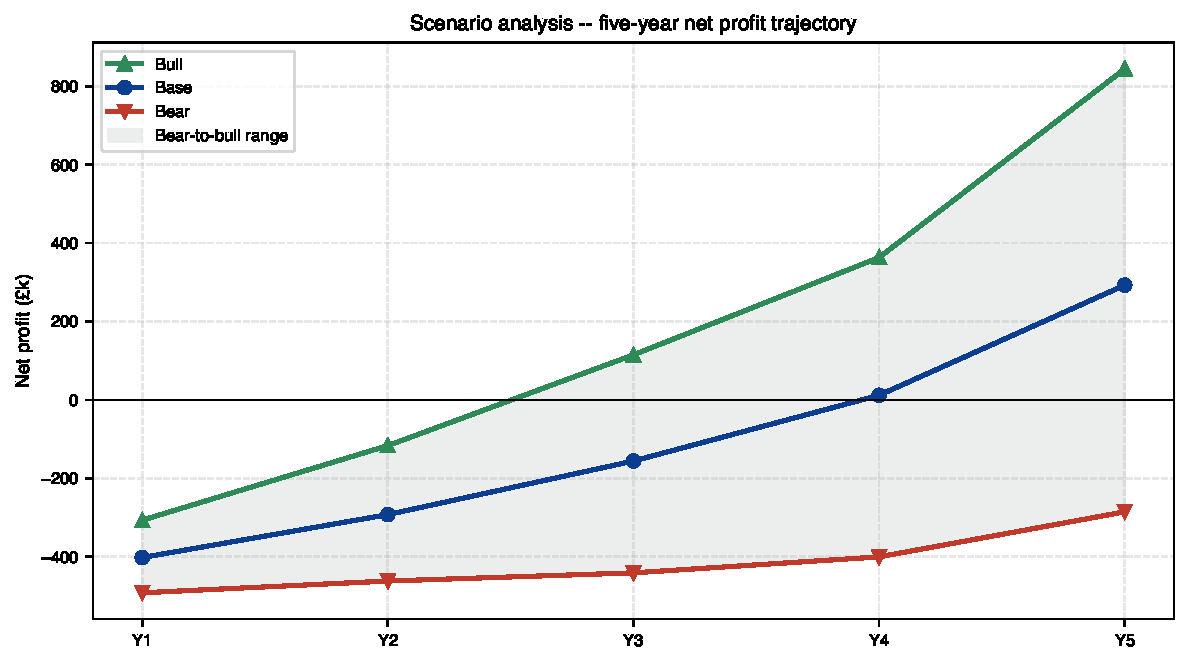
\includegraphics[width=\textwidth]{scenarios.pdf}
\caption{Scenario net-profit after tax (\pounds k, Y1--Y5). Bull reaches
  $+$\pounds844\,k by Y5; Bear stays loss-making ($-$\pounds285\,k)
  and would force a cost reset or bridge financing.}
\label{fig:scenarios}
\end{figure}

Section~\ref{sec:business_sensitivity} varies one driver at a time; Bull and
Bear add two compound cases that stress correlated downside/upside on the
dominant levers (days and blended day rate and variable cost), bracketing the
Base plan developed in Sections~\ref{sec:capex}--\ref{sec:cash_flow}:

\noindent
\begin{tabular}{@{}>{\raggedright\arraybackslash}p{0.47\textwidth}>{\raggedright\arraybackslash}p{0.47\textwidth}@{}}
\textbf{Bull:} $+25\%$ days, $+10\%$ rate, $-5\%$ variable cost. &
\textbf{Bear:} $-30\%$ days, $-10\%$ rate, $+10\%$ variable cost. \\
\end{tabular}

Bear is not a venture-sustainable path: cumulative loss exceeds the
\totalRaise{} equity stack. 

% ---------------------------------------------------------------------
\subsection{Minimum viable Commercial conditions}
\label{sec:mvc_conditions}
% ---------------------------------------------------------------------

Minimum viable commercial conditions (MVC) identify the operating limits at
which the financial model exhausts economic value (NPV hits 0) or liquidity
(end-Y2 cumulative cash hits 0).

\noindent The Bear scenario marks commercial failure; this section details
what happens short of full Bear but on the edge of viability.

\bigskip
\noindent\textbf{NPV${}=0$.}\par
\noindent
We stress sold days, blended day-rate, and
variable \pounds/day together, and also vary only sold days (the driver least
under management control), until NPV@20\% reaches zero; the model then implies
the following year-by-year values:

\begin{center}
\small
\begin{tabular}{rrrr|r}
\hline
\textbf{Y} &
\textbf{Joint} &
\textbf{Bl.\ \pounds/d} &
\textbf{Var.\ \pounds/d} &
\textbf{Sold Days Only} \\
\hline
1 & 30 & 6{,}883 & 2{,}489 & 27 \\
2 & 52 & 7{,}342 & 2{,}543 & 47 \\
3 & 82 & 7{,}801 & 2{,}597 & 73 \\
4 & 112 & 8{,}260 & 2{,}651 & 100 \\
5 & 165 & 8{,}718 & 2{,}705 & 146 \\
\hline
\end{tabular}
\end{center}

\noindent For this joint stress, end-Y2 cumulative cash is about
$-$\pounds133\,k. The Sold Days Only column shows an end-Y2 cumulative cash of $-$\pounds108\,k, so volume alone can
erase the Year-2 cushion at the NPV crossover.

Liquidity fails before NPV showing that NPV alone is misleading for viability. The model can
still show positive NPV while already in a incompatible cash model
unless more equity is raised, or costs are cut back.

\bigskip
\noindent\textbf{End-Y2 cumulative cash near zero.}\par
\noindent
A separate numerical solve targets end-Y2 cumulative cash $\approx$ \pounds0\,k
(the tightest point of the published cash forecast). The implied year-by-year
values are:

\begin{center}
\small
\begin{tabular}{rrrr|r}
\hline
\textbf{Y} &
\textbf{Joint} &
\textbf{Bl.\ \pounds/d} &
\textbf{Var.\ \pounds/d} &
\textbf{Sold Days Only} \\
\hline
1 & 36 & 7{,}282 & 2{,}366 & 34 \\
2 & 63 & 7{,}767 & 2{,}418 & 59 \\
3 & 100 & 8{,}253 & 2{,}469 & 93 \\
4 & 136 & 8{,}738 & 2{,}521 & 127 \\
5 & 200 & 9{,}223 & 2{,}572 & 187 \\
\hline
\end{tabular}
\end{center}

\noindent For joint stresses that result in end-Y2 cumulative cash = \pounds0\,k the
NPV is still about \pounds822\,k. The Sold Days Only model shows
NPV = \pounds731\,.

Viability in this model is more bounded by the pinch point at the end Year-2 cash flow than by NPV hitting 0.
%=====================================================================
\section{Financial risk: the downtime case}
\label{ch:risk_fin}
% =====================================================================

Section~\ref{sec:risk_analysis_strategic_tradeoffs} covers industry-level
risks. Here the focus is financial: if fleet maintenance fails
operationally, how much do NPV and EBIT suffer? For TaaS, revenue follows
utilisation (Section~\ref{sec:why_taas}), so that maintenance risk is the
main execution risk.

% ---------------------------------------------------------------------
\subsection{Downtime sensitivity -- quantifying the maintenance dependency}
\label{sec:downtime}
% ---------------------------------------------------------------------

Following Section~\ref{subsec:supply_chain_planning_framework}, we assume
$<$30-minute fleet recovery from any single failure; this underpins the
planned utilisation arrays in Table~\ref{tab:revenue}. Downtime is modelled
as a fractional reduction in billable days: a downtime rate of
$d\%$ delivers $(1-d)\cdot D_t$ billable days in year $t$. The fixed
cost base is unchanged (the crew is still paid while the vehicle is
grounded), so every percentage point of downtime translates
one-for-one into lost gross profit.

\begin{figure}[H]
\centering
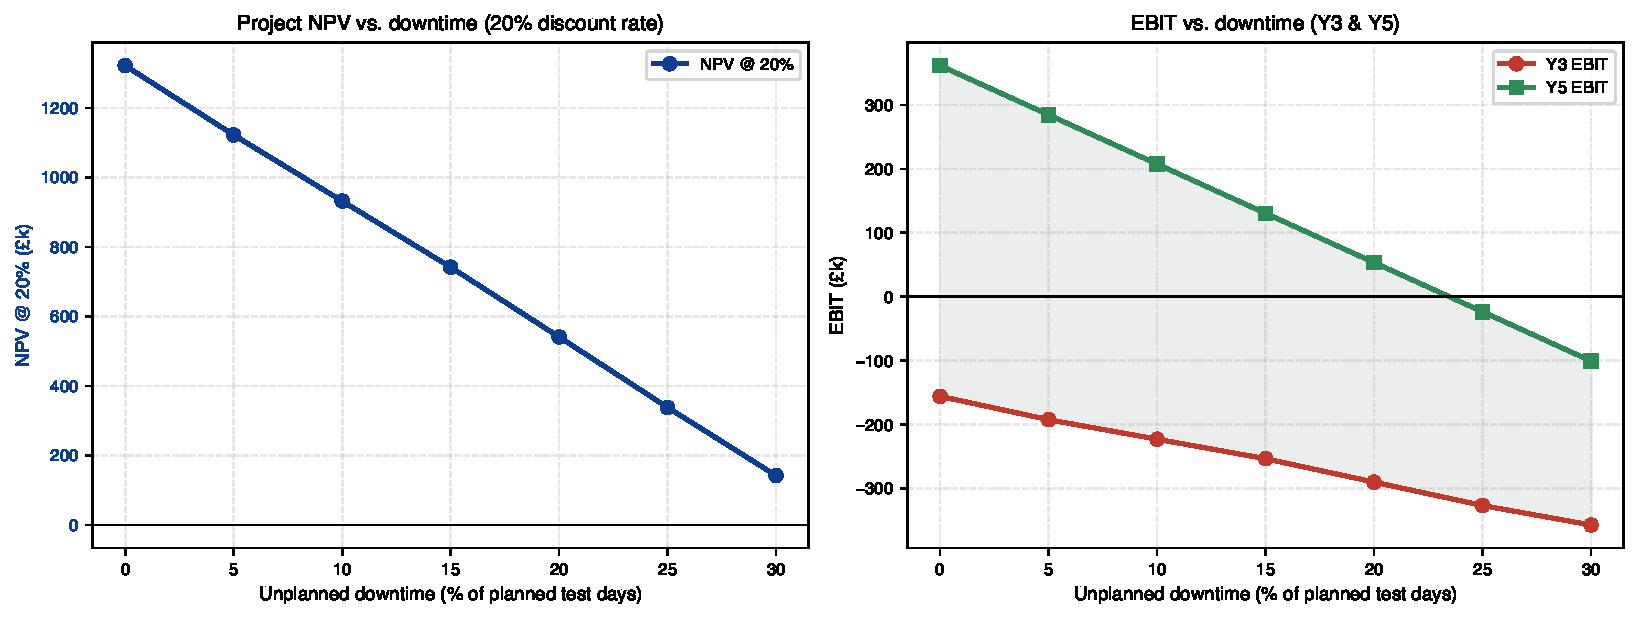
\includegraphics[width=\textwidth]{downtime.pdf}
\caption{Downtime sensitivity. Left: project NPV at 20\%
  discount rate as a function of unplanned downtime.
  Right: Y3 (red) and Y5 (green) EBIT for the same shock.}
\label{fig:downtime}
\end{figure}

\paragraph{Interpretation.}
\begin{tightitemize}
  \item \textbf{EBIT is brittle.} Y3 EBIT deteriorates from
        $-$\pounds156\,k to $-$\pounds357\,k as downtime rises
        from 0 to 30\%; Y5 EBIT turns negative at $\sim$20\%
        downtime.
  \item \textbf{NPV is less brittle -- but only as long as the
        exit multiple holds.} NPV@20\% falls from
        \pounds1.32\,M to \pounds0.14\,M at 30\% downtime, still
        positive but with little margin. If the downtime event
        also compresses the exit multiple
        (acquirers discount unreliability), NPV can flip negative
        at lower downtime levels.
  \item \textbf{Maintenance is cheap to fund but expensive to starve.}
        Relative to the recurring maintenance cash costs in the base plan,
        the losses from systematic downtime dominate: at 10\% downtime,
        \pounds190\,k of Y5 revenue, \pounds154\,k of Y5 EBIT, and
        \pounds390\,k of NPV@20\% are lost; at 20\% downtime those figures
        rise to \pounds418\,k, \pounds308\,k, and \pounds781\,k.
\end{tightitemize}

\paragraph{Implication for the maintenance budget.} The financial
cost of a 10\% systematic downtime (\pounds390\,k NPV reduction) is
more than double the total Y1 vehicle-maintenance contract
(\pounds20\,k) and an order of magnitude above the incremental
cost of a spare-vehicle strategy. Investment in maintenance
capability should be viewed as NPV-protection
value, not the headline opex line.

% ---------------------------------------------------------------------
\subsection{Financial risk:}
\label{sec:cash_risk}
% ---------------------------------------------------------------------

The cash forecast (Section~\ref{sec:cash_flow}) identified
end-Y2 cash balance of \pounds90\,k as the tightest point of the
plan. A compounded shock at that moment i.e. a
Series~A close three months late plus a reportable safety
incident, is sufficient to push the business into bridge-round
territory. Three specific financial exposures follow:

\begin{tightitemize}
  \item \textbf{Series~A timing.} Only \pounds90\,k buffer at
        Y2/Y3 boundary. Series~A prep therefore starts at Month~15
        to target a Q4-Y2 close; bridge-round authorisation is
        pre-negotiated with seed investors.
  \item \textbf{Reportable safety incident.} A single incident can
        increase insurance premium by $2$--$5\times$ (shifting the
        insurance line from $\sim$\pounds20\,k/year to
        $\sim$\pounds50--100\,k/year) and close the OEM
        supplier-approval pathway which may severely damage the utilisation ramp.
  \item \textbf{1st customer concentration.} In Y1,
        $>$30\% of revenue is from a single customer. The Series~A trigger thus requires \emph{two} cusotmer to reduce the risk of
        single-customer concentration.
\end{tightitemize}

% =====================================================================
\section{Funding strategy, valuation and financial KPIs}
\label{ch:funding}
% =====================================================================

% ---------------------------------------------------------------------
\subsection{Funding strategy and use of funds}
\label{sec:funding}
% ---------------------------------------------------------------------

The plan requires a total of \totalRaise of equity, in two
rounds.

\begin{tightitemize}
  \item \textbf{Seed, \seedRound at incorporation.} Used for Y1
        vehicle build (\capexPerVehicle), Y1 workshop (\pounds50\,k), and $\sim$18 months of runway
        ($\sim$\pounds600\,k). Indicative valuation
        \pounds4\,M $\Rightarrow$ 20\% equity round.
  \item \textbf{Series~A, \seriesARound at Q4-Y2 / Q1-Y3.} Used
        for the second-vehicle build, Y3--Y4 headcount additions
        (Sales, second test engineer), and a further $\sim$18
        months of runway. Indicative pre-money valuation
        \pounds6\,M $\Rightarrow$ 20\% equity round.
\end{tightitemize}

\noindent The \textbf{Series~A trigger is revenue-based, not
runway-based}: $\geq$\pounds400\,k ARR and $\geq$ 2 retainer
customers. Missing the trigger implies a bridge round from seed
investors rather than a Series~A at a compressed valuation; the
seed term sheet should pre-authorise this bridge.

\medskip

\noindent \textbf{Unit economics.} Using an average customer of
$\sim$8 test days/year at a blended day-rate of \pounds7.5\,k,
three-year average relationship, and 70\% revenue-weighted gross
margin:

\begin{equation}
\mathrm{LTV} = (8 \times 7{,}500) \times 3 \times 0.70 = \ltv,
\qquad
\frac{\mathrm{LTV}}{\mathrm{CAC}} = \ltvCac,
\qquad
\mathrm{Payback} = \paybackMonths \text{ months}.
\end{equation}

Both metrics clear standard B2B-services investability
thresholds~\cite{gompers2020} by a wide margin; a doubling of CAC
still clears the 3$\times$ LTV/CAC rule.

% ---------------------------------------------------------------------
\subsection{Valuation (comparable multiples)}
\label{sec:valuation}
% ---------------------------------------------------------------------

Indicative Y5 valuation uses listed-peer EV/Revenue multiples,
benchmarked against AB~Dynamics (LSE:~ABDP), Spirent Communications
(LSE:~SPT), and AVL~List~\cite{abdynamics_ar2024,avl_profile}.

% --- BEGIN INLINE: HarryEmes/Business/tables/valuation.tex ---
\begin{table}[H]
\centering
\small
\caption{Comparable-multiples valuation. Year-5 forecast revenue 
(\pounds2.1M) multiplied by peer EV/Revenue multiples 
gives the indicative Year-5 enterprise-value range.}
\label{tab:valuation}
\begin{tabular}{lcr}
\toprule
\textbf{Peer} & \textbf{EV / Revenue} & \textbf{Implied EV (\pounds M)} \\
\midrule
AB Dynamics (LSE: ABDP, 2024) & 3.5$\times$ & 7.3 \\
Spirent Communications (LSE: SPT) & 2.2$\times$ & 4.6 \\
AVL List (private, Refinitiv est.) & 1.8$\times$ & 3.8 \\
Peer-group median & 2.5$\times$ & 5.2 \\
\bottomrule
\end{tabular}
\end{table}
% --- END INLINE: HarryEmes/Business/tables/valuation.tex ---
At the peer-group median of $2.5\times$ Y5 revenue, the indicative
Y5 enterprise value is \terminalValue. The NPV  is robust within this
band but sensitive to a compression below the peer-group floor
(AVL at 1.8$\times$).

% =====================================================================
\section{Conclusions and Recommendations}
\label{ch:concl}
% =====================================================================

Our business model clears standard
thresholds: project NPV of \npvBase at a 20\%
VC-central discount rate, IRR of \irr, and break-even in
\breakEvenYear at \breakEvenDays test days/year. The financial
structure is typical of a capex-inverted TaaS: loss
through Y3, cash-thin at the Y2/Y3 boundary, and NPV dominated by
the present value of the Y5 exit. Three recommendations follow, each with the financial action it drives.

\begin{tightenumerate}
  \item \textbf{Invest ahead of the maintenance-protocol budget.}
        A 10\% systematic downtime costs \pounds390\,k of NPV which is
        an order of magnitude above the baseline maintenance-opex
        line. \emph{Y1 action}: scope a spare-vehicle strategy
        and benchmark it against the NPV-protection value, not
        the accounting opex.
  \item \textbf{Prioritise pricing discipline over cost discipline
        in management incentives.} The sensitivity ranking
        identifies blended day-rate as the highest-leverage
        financial driver; the commercial team should be
        compensated on mix-shift to Silver/Gold, not only on
        volume. \emph{Y1 action}: incentive plan pays on blended
        day-rate as well as bookings.
  \item \textbf{Protect the Y2/Y3 cash boundary at all costs.}
        Only \pounds90\,k of buffer; compound shocks can
        cascade into a bridge round at a compressed valuation.
        \emph{Y1 action}: target Series~A close at Q4-Y2, not Y3.
\end{tightenumerate}

\medskip

\noindent The TaaS financial structure is viable and
defensible. The single biggest threat to financial returns is
the execution of the recovery assumptions in Section~\ref{subsec:supply_chain_planning_framework} that the model assumes.
Protecting that assumption is both the cheapest and
highest-leverage action we can take.

% =====================================================================
\compactbib
% --- END INLINE: HarryEmes/Business/harry_business_body.tex ---
\end{refsection}

\end{document}
